% This is the Reed College LaTeX thesis template. Most of the work
% for the document class was done by Sam Noble (SN), as well as this
% template. Later comments etc. by Ben Salzberg (BTS). Additional
% restructuring and APA support by Jess Youngberg (JY).
% Your comments and suggestions are more than welcome; please email
% them to cus@reed.edu
%
% See http://web.reed.edu/cis/help/latex.html for help. There are a
% great bunch of help pages there, with notes on
% getting started, bibtex, etc. Go there and read it if you're not
% already familiar with LaTeX.
%
% Any line that starts with a percent symbol is a comment.
% They won't show up in the document, and are useful for notes
% to yourself and explaining commands.
% Commenting also removes a line from the document;
% very handy for troubleshooting problems. -BTS

% As far as I know, this follows the requirements laid out in
% the 2002-2003 Senior Handbook. Ask a librarian to check the
% document before binding. -SN

%%
%% Preamble
%%
% \documentclass{<something>} must begin each LaTeX document

\documentclass[oneside]{report}
\usepackage{Suthesis-2e}
% Packages are extensions to the basic LaTeX functions. Whatever you
% want to typeset, there is probably a package out there for it.
% Chemistry (chemtex), screenplays, you name it.
% Check out CTAN to see: http://www.ctan.org/
%%
\usepackage{graphicx,latexsym}
\usepackage{amsmath}
\usepackage{amssymb,amsthm}
\usepackage{longtable,booktabs,setspace}
\usepackage{chemarr} %% Useful for one reaction arrow, useless if you're not a chem major
\usepackage[hyphens]{url}
% Added by CII
\usepackage[draft]{hyperref}
\usepackage{lmodern}
\usepackage{float}
\floatplacement{figure}{H}
% End of CII addition
\usepackage{rotating}

% Next line commented out by CII
%%% \usepackage{natbib}
% Comment out the natbib line above and uncomment the following two lines to use the new
% biblatex-chicago style, for Chicago A. Also make some changes at the end where the
% bibliography is included.
%\usepackage{biblatex-chicago}
%\bibliography{thesis}


% Added by CII (Thanks, Hadley!)
% Use ref for internal links
\renewcommand{\hyperref}[2][???]{\autoref{#1}}
\def\chapterautorefname{Chapter}
\def\sectionautorefname{Section}
\def\subsectionautorefname{Subsection}
% End of CII addition

% Added by CII
\usepackage{caption}
\captionsetup{width=5in}
% End of CII addition

% \usepackage{times} % other fonts are available like times, bookman, charter, palatino

% Syntax highlighting #22

% To pass between YAML and LaTeX the dollar signs are added by 
\setstretch{1.6}

\usepackage{amsthm}
\newtheorem{theorem}{Theorem}[chapter]
\newtheorem{lemma}{Lemma}[chapter]
\theoremstyle{definition}
\newtheorem{definition}{Definition}[chapter]
\newtheorem{corollary}{Corollary}[chapter]
\newtheorem{proposition}{Proposition}[chapter]
\theoremstyle{definition}
\newtheorem{example}{Example}[chapter]
\theoremstyle{definition}
\newtheorem{exercise}{Exercise}[chapter]
\theoremstyle{remark}
\newtheorem*{remark}{Remark}
\newtheorem*{solution}{Solution}
\begin{document}
\title{Learning Disjunction}
\author{Masoud Jasbi}
% The month and year that you submit your FINAL draft TO THE LIBRARY (May or December)
\date{May 2018}
\dept{Linguistics}
\principaladviser{Eve V. Clark}
\firstreader{Christopher Potts}
\secondreader{Michael Frank}
  \thirdreader{Ellen Markman} %if needed

% if you're writing a thesis in an interdisciplinary major,
% uncomment the line below and change the text as appropriate.
% check the Senior Handbook if unsure.
%\thedivisionof{The Established Interdisciplinary Committee for}
% if you want the approval page to say "Approved for the Committee",
% uncomment the next line
%\approvedforthe{Committee}

% Added by CII
%%% Copied from knitr
%% maxwidth is the original width if it's less than linewidth
%% otherwise use linewidth (to make sure the graphics do not exceed the margin)
\makeatletter
\def\maxwidth{ %
  \ifdim\Gin@nat@width>\linewidth
    \linewidth
  \else
    \Gin@nat@width
  \fi
}
\makeatother

\renewcommand{\contentsname}{Contents}
% End of CII addition

\setlength{\parskip}{0pt}

% Added by CII

\providecommand{\tightlist}{%
  \setlength{\itemsep}{0pt}\setlength{\parskip}{0pt}}




\beforepreface
\prefacesection{Abstract}
The preface pretty much says it all. \par

Second paragraph of abstract starts here.

\prefacesection{Dedication}

%\prefacesection{}
%This thesis is dedicated to 
\prefacesection{Acknowledgments}


\afterpreface


\chapter*{Introduction}\label{introduction}
\addcontentsline{toc}{chapter}{Introduction}

In the literature on word learning, the story goes that one day, a
linguist with great mastery of phonetics and phonology, heard of a
people with an unknown language. She immediately packed her bags and
traveled to learn about this new language. When she arrived, she saw a
man walking down the road. Suddenly a rabbit scurried by. The man saw
the rabbit and said ``gavagai''. The linguist immediately pulled out her
notebook. As an excellent phonetician with trained ears for detecting
linguistic sounds, she wrote down the phonetic transcription of what she
heard with great confidence. It was only when she tried to write the
meaning that doubt and uncertainty seeped in. ``Does \emph{gavagai} mean
rabbit?'', she whispered quietly. As a good scientist, she could see
that her observation was compatible with a large number of hypotheses
for the meaning of \emph{gavagai}: ``white-thing'', ``furry thing'',
``animal'', ``fast'', ``what was that?'', ``oh gosh!'',
``rabbit-on-the-road'', and even ``undetached rabbit parts''! She shook
her head and let out a sigh. She found this ``referential uncertainty''
challenging (Quine, 1960).

Unlike what most of us think, the story did not end there. The linguist
continued with her observations and soon she learned the meaning of
\emph{gavagai} as well as many other words, mostly nouns, adjectives,
and verbs. But soon she encountered a new challenge. One day when she
was walking down the same road with the same man she met the first day,
there was some movement in the nearby bushes. The man pointed to the
bushes and said: ``tonomi yok gavagai''. She now knew that
\emph{gavagai} meant rabbit. She also knew that \emph{tonomi} is another
animal. But she had never heard the word \emph{yok} before. What did
\emph{yok} mean? ``Maybe the man saw an animal and was not sure whether
it was a gavagai \textbf{or} a tonomi'', she thought. However, the man
did not sound uncertain. ``What if he was trying to say that the animal
was a gavagai \textbf{and not} a tonomi \ldots{} or maybe he saw two
animals and wanted to let me know that there was a gavagai \textbf{and}
a tonomi in the bushes.'' It was also possible that by that time, the
man knew she was trying to learn their language and wanted to let her
know that ``gavagai'' and ``tonomi'' are terms that apply to the same
animal; something like: ``this is called a gavagai \textbf{or} a
tonomi''. The linguist in our story sighed again. Even though she knew
the meaning of words for things and actions, she needed to know the
meaning of words that put them together to convey larger concepts.
Legend has it that she did not go home until she discovered the meaning
of every ``function word'' in this new language.

\section{Word Learning}\label{word-learning}

Learning the meaning of a word is often construed as mapping a
linguistic form such as \emph{gavagai} to a concept/meaning such as
``rabbit''. This mapping process is described in three stages: First the
learner isolates the word form; then s/he isolates a meaning from a set
of possible meanings; and finally s/he maps (or associates) the isolated
word to the isolated meaning (E. V. Clark, 1993). A fundamental question
in the acquisition of meaning concerns the second step of mapping: how
do children select the right meaning of a word from a set of candidate
meanings? Quine (1960)'s thought experiment with the linguist and the
new language showed that this is not a trivial task. In any given
context, a word is compatible with many possible meanings. The problem
of selecting the right meaning for a given word is called the ``mapping
problem'' or the ``gavagai problem''.

Solutions to the mapping problem often place constraints on either the
hypothesis space or the structure of the lexicon to make word learning
tractable (E. V. Clark, 1993). For example, the taxonomic constraint
(Markman \& Hutchinson, 1984) proposes that children generate semantic
hypotheses for nouns that denote a set of taxonomically related entities
and do not hypothesize meanings that capture sets of entities with
thematic relations. For example, given the word \emph{gavagai}, children
hypothesize the meaning ``rabbit'' which denotes the set of rabbits
(taxonomically related) but not ``rabbit and carrot'' (thematically
related). Therefore, the taxonomic constraint limits the space of
hypotheses that the learner entertains. On the other hand, the mutual
exclusivity constraint (Markman \& Wachtel, 1988) as well as the
pragmatic principle of contrast (E. V. Clark, 1987) limit the structure
of the lexicon such that two words are not mapped into the same meaning.
This constraint on the lexicon makes the word learning task easier by
removing hypotheses that are already associated with learned words.

Another solution to the mapping problem is to propose cues that bias the
learner towards one hypothesis rather than another. For example,
socio-pragmatic cues such as pointing and joint-attention (D. A.
Baldwin, 1993; E. V. Clark, 2009; Tomasello, 2003) direct the learner to
bias one hypothesis over others. For example, given a rabbit and a cat,
the speaker pointing to the rabbit and saying \emph{gavagai} biases the
learner to map the meaning of \emph{gavagai} to ``rabbit'' rather than
``cat''. Learning models can also integrate cues and constraints to
develop a learning account that uses multiple cues to home in on the
target meaning of a word (Hollich et al., 2000).

While there has been a large body of research on the set of cues and
constraints that aid the acquisition of content word semantics, cues
that assist the acquisition of function words have not received as much
attention. This dissertation aims at advancing a multiple cue-based
acquisition of functions words by investigating the acquisition of the
disjunction word \emph{or}. In the next section I explain the scope of
this dissertation within a program of research that aims at developing a
cue-based acquisition of function words.

\section{Defining the Scope}\label{defining-the-scope}

The lexicon of a language can be divided into two groups of words:
content words and function words. Content words consist of nouns (e.g.
\emph{cat}, \emph{Bob}, \emph{freedom}), verbs (e.g. \emph{run},
\emph{blink}, \emph{imagine}), adjectives (e.g. \emph{happy},
\emph{red}, \emph{fake}), and adverbs (e.g. \emph{fast}, \emph{quietly},
\emph{quickly}). Function words include articles (e.g. \emph{a},
\emph{the}), quantifiers (e.g. \emph{some}, \emph{most}, \emph{all}),
prepositions (e.g. \emph{in}, \emph{on}, \emph{at}), pronouns (e.g.
\emph{he}, \emph{they}, \emph{her}), auxiliary verbs (e.g. \emph{did},
\emph{can}, \emph{am/is/are}), connectives (e.g. \emph{or}, \emph{if},
\emph{because}), interrogatives (e.g. \emph{who}, \emph{what},
\emph{when}), among others. Function words differ from content words in
(at least) five crucial ways. First, function words are phonologically
simpler than content words (Shi, 1996). Second, even though content
words vastly outnumber function words, function words are a lot more
frequent. Third, while content words frequently admit new members,
function words rarely do so. This is why content words are considered an
open class in the lexicon while function words are called a
closed-class. Fourth, the common intuition is that content words carry
more meaning and the concepts they denote are more tangible. The
meanings of function words, however, are subtle and abstract. Finally,
function words appear in children's speech later than content words.

Even though content words commonly steal the spotlight, the unique
properties of function words make them a valuable resource to linguists
and cognitive scientists. They are few in number, extremely frequent,
and very abstract in meaning. They are the essential nuts and bolts that
combine smaller concepts to form larger thoughts. They provide crucial
information on the structure and inner workings of human language and
mind. The crosslinguistic and psycholinguistic study of function words
provides us with an exceptional window into structure and building
blocks of the human thought and reasoning.

Within function words, logical connectives \emph{and}, \emph{or},
\emph{not}, \emph{if}, have received considerable attention in the
linguistic and psychological literature due to the foundational role
that the concepts of conjunction, disjunction, negation, and implication
play in logic and mathematics. In linguistics and philosophy, a large
body of research has investigated the connections between the meanings
of these words and their corresponding operators in formal logics.
Similarly in psychology, there has been substantial research on
children's development and adults comprehension of logical concepts and
logical reasoning. This dissertation focuses on the acquisition of the
disjunction word \emph{or} by preschool children. It proposes a learning
account for \emph{or} (and its counterpart \emph{and}), that can be
expanded in the future to linguistic connectives in general such as
\emph{but}, \emph{because}, \emph{yet}, \emph{so}, \emph{after},
\emph{before}, \emph{although}, \emph{however}, etc.

\section{The Structure of the
Dissertation}\label{the-structure-of-the-dissertation}

This dissertation consists of four parts: literature review (Chapters
\ref{sempragLit} and \ref{devoLit}), comprehension studies (Chapter
\ref{comprehension}), corpus studies (Chapter \ref{corpus}), and
modeling (Chapter \ref{corpus}). Starting with the literature review,
Chapter \ref{sempragLit} provides an overview of the semantics and
pragmatics of \emph{or} in English. The main focus of the chapter is the
empirical discoveries about the interpretations of disjunction in
different linguistic and nonlinguistic contexts. The chapter shows that
on the surface, a disjunction like ``A or B'' can be interpreted as
inclusive disjunction, exclusive disjunction, or a conjunction. These
interpretations are often accompanied by ignorance inferences (the
speaker does not know which option is true) or indifference inferences
(the speaker does not care which option is true). The chapter discusses
the factors that affect the interpretation of \emph{or} in a given
context. These factors include conversational principles, entailment
environment, modality, disjunct semantics, intonation, syntax,
metalinguistic speech acts, and some specific constructions such as
embedded imperatives and unconditionals. The chapter argues that these
factors can act as cues for the acquisition and interpretation of
disjunction.

Chapter \ref{devoLit} provides an overview of research on the
acquisition and interpretation of disjunction in children. It discusses
three accounts of children's acquisition of logical connectives:
development of logical reasoning, usage-based account, and logical
nativism. The first two consider logical concepts such as disjunction as
emergent from more primitive concepts such as ``choice''. Logical
nativism, however, proposes that humans are born with logical concepts
necessary for linguistic interpretation, as part of their Universal
Grammar. The first two accounts -- development of logical reasoning and
the usage-based account-- predict that children start with an exclusive
interpretation of disjunction and only later, around age 5 or 6, do they
interpret \emph{or} in its ``logical'' inclusive sense. The nativist
account predicts that children interpret \emph{or} as inclusive
disjunction from the beginning and only later with the development of
pragmatic reasoning, they derive the exclusive interpretation.

Chapter \ref{comprehension}, presents three studies on adults' and
children's comprehension of \emph{or} in simple existential sentences
(``there is A or B''). The first study tests adults comprehension of
discussion using two and three-alternative forced-choice truth-value
judgment tasks (2AFC and 3AFC TVJTs). The 2AFC task showed that adults
interpret \emph{and} as conjunction and \emph{or} as inclusive
disjunction. The 3AFC task showed that adults do not consider a
disjunction completely felicitous when both disjuncts are true. The
second study used a similar 3AFC task to test three-to-five year old
children's comprehension of \emph{and} and \emph{or}. The study also
analyzed and categorized children's open-ended spontaneous feedback in
the task. Children's interpretations were similar to adults except in
cases where both disjuncts were true. In such cases, children's forced
choice responses showed no sign of infelicity while their spontaneous
feedback showed such signs: children corrected the utterance with
\emph{or} and suggested that \emph{and} should have been used instead.
Study 3 used a two-alternative forced choice (2AFC) task and categorized
children's open-ended feedback. The two-alternative forced choice task
showed similar results to adults and the study replicated children's
open-ended feedback in study 2: children provided corrections to the
utterance when both disjuncts were true and offered the connective
\emph{and}. Overall the results suggested that three-to-five year old
children's interpretations of disjunction do not substantially differ
from those of adults.

Chapter \ref{corpus} presents two corpus studies. First, it presents a
large-scale analysis of parents and children's productions of \emph{and}
and \emph{or}. The results show that children start producing \emph{and}
between the first and the second years of their lives and reach their
parents rate of \emph{and} production around their third birthday. For
disjunction, children start producing \emph{or} between two and three
years of age and by the time they are four, they reach a constant rate
of \emph{or} production. This rate is slightly lower than that of their
parents. Overall the results of this study support the findings of
Chapter \ref{comprehension}: by age four, children develop a good
understanding of connectives \emph{and} and \emph{or}. The second study
selected a subset of \emph{and} and \emph{or} in child-directed speech
for children between the ages of one and three. The study annotated
utterances containing \emph{and} and \emph{or} for seven cue categories:
their interpretation (exclusive, inclusive, conjunction), intonation,
utterance type (declarative, question, imperative), syntax, consistency
(clean or dirty vs.~clean or tidy), communicative function, and answer
type (correct vs.~incorrect answers to questions with \emph{or}). The
results showed that intonation, and consistency play a large role in
determining the interpretation of a disjunction. The results also show
that around age 2, children start providing appropriate answers to
questions with disjunction. The findings of this chapter suggest that
children develop their understanding of disjunction mostly between their
second and fourth birthday.

Finally, in chapter \ref{modeling}, I report the results of applying
random decision forests (Ho, 1995) to the annotation dataset. The
modeling study uses the annotation categories in study 2 of Chapter
\ref{corpus} to learn a decision structure to successfully interpret
conjunction and disjunction. The results show that using the cues
proposed in Chapter \ref{corpus}, a random forest can reach above 85\%
accuracy in classifying the correct interpretation of a conjunction or a
disjunction. Given the results of the annotation study and the
computational modeling, Chapter \ref{conclusions} provides a learning
account for connectives \emph{and} and \emph{or}.

\chapter{Interpretations of Disjunction}\label{sempragLit}

\section{Introduction}\label{introduction-1}

Despite its modest appearance, the word \emph{or} has been a major
trouble maker for formal theories of meaning. Perhaps the main reason is
that capturing its meaning has always seemed within the reach of formal
accounts at the time, yet more examination has shown that \emph{or} is
much more complex than expected. Consequently, few words have managed to
prove as influential as \emph{or} in advancing formal semantics and
pragmatics. This chapter is dedicated to the semantics and pragmatics of
disjunction, and specifically \emph{or} in English. My primary goal is
to provide an overview of the empirical discoveries in the
interpretation of \emph{or} in adult language before moving to
disjunction in child language acquisition.

In discussing linguistics meaning, often different words are used to
refer to different types of meaning. Here I clarify my terminology. In
what follows, I may use the terms ``meaning'', ``implicature'',
``inference'', ``implication'', and ``interpretation''. I use the term
``meaning'' to refer to ``literal meaning'': the meaning of words and
word combinations in their most ``literal'', least context-dependent,
and least enriched version. Most of the time my usage of ``meaning''
refers to ``lexical meaning''. I use ``implicature'' (conversational)
when the meaning is considered to be derived from literal meaning via
the Gricean cooperative principle and its associated conversational
maxims (Grice, 1989). The term ``inference'' is used more generally to
refer to any type of meaning that is derived from literal meaning using
some form of reasoning. I use ``implication'' to refer to all linguistic
meaning regardless of the source and theoretical status. Therefore,
literal meanings, implicatures, and inferences are all implications.
Finally, I use interpretation in the broadest and most theoretically
neutral way to include all types of meaning; linguistic or
non-linguistic.

In what follows, I start with the discussion of disjunction in logic and
philosophy. Disjunction has enjoyed a great deal of investigation in
these fields and it would not be possible to understand current
semantics and pragmatics of disjunction without first understanding its
logical background. Then I move to the discussion of disjunction in
language, and more specifically \emph{or} in English. I show that since
the early linguistic investigations, two different approaches to the
meaning of disjunction have co-existed: first lexical ambiguity
accounts, and second Gricean accounts. I explain that lexical ambiguity
accounts consider \emph{or} ambiguous between several meanings or senses
while the Gricean accounts propose a single meaning for \emph{or} and
derive different interpretations of a disjunction from other linguistic
and conversational factors. Then I enumerate some of the factors that
affect the interpretation of disjunction. I argue that these factors
provide a starting point for a cue-based acquisition of disjunction.

\section{Disjunction in Logic}\label{logic}

The first explicit account of propositional connectives in logic was
developed by Stoic philosophers (3BC - 3AD) (Bonevac \& Dever, 2012).
They divided logical propositions into simple (atomic) and complex
(molecular) propositions. Complex propositions were made of simple
propositions connected by connective such as conjunction and
disjunction. Similar to logical systems today, they defined these
connectives in terms of the truth conditions of the propositions they
connect. A conjunction was considered true when all propositions are
true and false otherwise. Disjunction, however, received two
definitions: exclusive disjunction and inclusive disjunction. Exclusive
disjunction is true when exactly one proposition is true and the rest
are false. Inclusive disjunction is true when at least one proposition
is true, the rest may be true or false. Table \ref{tab:truthtable} shows
the truth conditions for binary conjunction (\(\land\)), exclusive
disjunction (\(\oplus\)), and inclusive disjunction (\(\lor\))\footnote{Binary
  exclusive disjunction has an ``odd property''" in that linking a
  sequence of exclusive disjuncts results in a disjunction that is true
  if and only if odd number of disjuncts are true. This is not the case
  for the Stoic version of disjunction which is not a binary operator.}.
\begin{longtable}[]{@{}ccccc@{}}
\caption{\label{tab:truthtable} Truth conditions for conjunction and
disjunction in classical logic}\tabularnewline
\toprule
\(\phi\) & \(\psi\) & \((\phi \land \psi)\) & \((\phi \oplus \psi)\) &
\((\phi \lor \psi)\)\tabularnewline
\midrule
\endfirsthead
\toprule
\(\phi\) & \(\psi\) & \((\phi \land \psi)\) & \((\phi \oplus \psi)\) &
\((\phi \lor \psi)\)\tabularnewline
\midrule
\endhead
T & T & T & F & T\tabularnewline
T & F & F & T & T\tabularnewline
F & T & F & T & T\tabularnewline
F & F & F & F & F\tabularnewline
\bottomrule
\end{longtable}
It is important to note that there are entailment relations between the
connectives in Table \ref{tab:truthtable}. A proposition \(\phi\)
entails another proposition \(\psi\) if in all situations that \(\phi\)
is true \(\psi\) is true as well. Conjunction of two propositions
entails their inclusive disjunction but not the other way round. When
the conjunction is true (row 1), the inclusive disjunction is also true
but there are situations where inclusive disjunction is true but the
conjunction is false (rows 2 and 3). Similarly, exclusive disjunction
entails inclusive disjunction but not the other way round. This is
because in every situation that exclusive disjunction is true, inclusive
disjunction is also true but there is one situation where inclusive
disjunction is true but exclusive disjunction is not. Conjunction and
exclusive disjunction stand in contradiction to each other. If the
conjunction of two propositions is true then the exclusive disjunction
is false and if the exclusive disjunction is true then their conjunction
is false. Figure \ref{fig:entailmentFigure} shows propositions as sets
of situations in which they are true. The entailment relations can be
seen as inclusion: a proposition that is contained within another
proposition entails it. Exclusive disjunction and conjunction are both
contained within inclusive disjunction and they both entail it.
\begin{figure}[tb]

{\centering 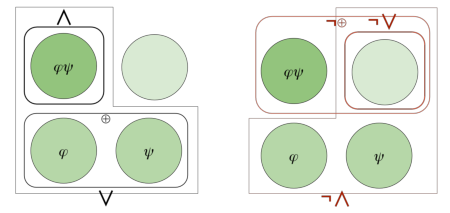
\includegraphics{figs/entailmentFigure-1} 

}

\caption{The relation betwen conjunction, inclusive disjunction, exclusive disjunction, and their negations.}\label{fig:entailmentFigure}
\end{figure}
Negation in classical logic is a unary operator that flips the truth
value of a proposition. Figure \ref{fig:entailmentFigure} also shows the
negation of conjunction and two types of disjunction. Negated inclusive
disjunction is contained within negated conjunction and negated
exclusive disjunction; consequently it entails them. Table
\ref{tab:truthtable} shows the meaning of negative atomic propositions
(\(\lnot \phi\), \(\lnot \psi\)), negative inclusive disjunctions
(\(\lnot (\phi \lor \psi)\)), negative conjunctions
(\(\lnot (\phi \land \psi)\)), inclusive disjunction of negative
propositions (\(\lnot \phi \lor \lnot \psi\)), the conjunction of
negative propositions (\(\lnot \phi \land \lnot \psi\)), negative
exclusive disjunction, and exclusive disjunction of negative
propositions.
\begin{longtable}[]{@{}cccccccccc@{}}
\caption{\label{tab:truthtable} Truth conditions for statements that involve
the interaction of conjunction and disjunction with negation in
classical logic.}\tabularnewline
\toprule
\begin{minipage}[b]{0.04\columnwidth}\centering\strut
\(\phi\)\strut
\end{minipage} & \begin{minipage}[b]{0.04\columnwidth}\centering\strut
\(\psi\)\strut
\end{minipage} & \begin{minipage}[b]{0.04\columnwidth}\centering\strut
\(\lnot \phi\)\strut
\end{minipage} & \begin{minipage}[b]{0.04\columnwidth}\centering\strut
\(\lnot \psi\)\strut
\end{minipage} & \begin{minipage}[b]{0.08\columnwidth}\centering\strut
\(\lnot (\phi \lor \psi)\)\strut
\end{minipage} & \begin{minipage}[b]{0.08\columnwidth}\centering\strut
\(\lnot (\phi \land \psi)\)\strut
\end{minipage} & \begin{minipage}[b]{0.08\columnwidth}\centering\strut
\(\lnot \phi \lor \lnot \psi\)\strut
\end{minipage} & \begin{minipage}[b]{0.08\columnwidth}\centering\strut
\(\lnot \phi \land \lnot \psi\)\strut
\end{minipage} & \begin{minipage}[b]{0.09\columnwidth}\centering\strut
\(\lnot (\phi \oplus \psi)\)\strut
\end{minipage} & \begin{minipage}[b]{0.08\columnwidth}\centering\strut
\(\lnot \phi \oplus \lnot \psi\)\strut
\end{minipage}\tabularnewline
\midrule
\endfirsthead
\toprule
\begin{minipage}[b]{0.04\columnwidth}\centering\strut
\(\phi\)\strut
\end{minipage} & \begin{minipage}[b]{0.04\columnwidth}\centering\strut
\(\psi\)\strut
\end{minipage} & \begin{minipage}[b]{0.04\columnwidth}\centering\strut
\(\lnot \phi\)\strut
\end{minipage} & \begin{minipage}[b]{0.04\columnwidth}\centering\strut
\(\lnot \psi\)\strut
\end{minipage} & \begin{minipage}[b]{0.08\columnwidth}\centering\strut
\(\lnot (\phi \lor \psi)\)\strut
\end{minipage} & \begin{minipage}[b]{0.08\columnwidth}\centering\strut
\(\lnot (\phi \land \psi)\)\strut
\end{minipage} & \begin{minipage}[b]{0.08\columnwidth}\centering\strut
\(\lnot \phi \lor \lnot \psi\)\strut
\end{minipage} & \begin{minipage}[b]{0.08\columnwidth}\centering\strut
\(\lnot \phi \land \lnot \psi\)\strut
\end{minipage} & \begin{minipage}[b]{0.09\columnwidth}\centering\strut
\(\lnot (\phi \oplus \psi)\)\strut
\end{minipage} & \begin{minipage}[b]{0.08\columnwidth}\centering\strut
\(\lnot \phi \oplus \lnot \psi\)\strut
\end{minipage}\tabularnewline
\midrule
\endhead
\begin{minipage}[t]{0.04\columnwidth}\centering\strut
T\strut
\end{minipage} & \begin{minipage}[t]{0.04\columnwidth}\centering\strut
T\strut
\end{minipage} & \begin{minipage}[t]{0.04\columnwidth}\centering\strut
F\strut
\end{minipage} & \begin{minipage}[t]{0.04\columnwidth}\centering\strut
F\strut
\end{minipage} & \begin{minipage}[t]{0.08\columnwidth}\centering\strut
F\strut
\end{minipage} & \begin{minipage}[t]{0.08\columnwidth}\centering\strut
F\strut
\end{minipage} & \begin{minipage}[t]{0.08\columnwidth}\centering\strut
F\strut
\end{minipage} & \begin{minipage}[t]{0.08\columnwidth}\centering\strut
F\strut
\end{minipage} & \begin{minipage}[t]{0.09\columnwidth}\centering\strut
T\strut
\end{minipage} & \begin{minipage}[t]{0.08\columnwidth}\centering\strut
F\strut
\end{minipage}\tabularnewline
\begin{minipage}[t]{0.04\columnwidth}\centering\strut
T\strut
\end{minipage} & \begin{minipage}[t]{0.04\columnwidth}\centering\strut
F\strut
\end{minipage} & \begin{minipage}[t]{0.04\columnwidth}\centering\strut
F\strut
\end{minipage} & \begin{minipage}[t]{0.04\columnwidth}\centering\strut
T\strut
\end{minipage} & \begin{minipage}[t]{0.08\columnwidth}\centering\strut
F\strut
\end{minipage} & \begin{minipage}[t]{0.08\columnwidth}\centering\strut
T\strut
\end{minipage} & \begin{minipage}[t]{0.08\columnwidth}\centering\strut
T\strut
\end{minipage} & \begin{minipage}[t]{0.08\columnwidth}\centering\strut
F\strut
\end{minipage} & \begin{minipage}[t]{0.09\columnwidth}\centering\strut
F\strut
\end{minipage} & \begin{minipage}[t]{0.08\columnwidth}\centering\strut
T\strut
\end{minipage}\tabularnewline
\begin{minipage}[t]{0.04\columnwidth}\centering\strut
F\strut
\end{minipage} & \begin{minipage}[t]{0.04\columnwidth}\centering\strut
T\strut
\end{minipage} & \begin{minipage}[t]{0.04\columnwidth}\centering\strut
T\strut
\end{minipage} & \begin{minipage}[t]{0.04\columnwidth}\centering\strut
F\strut
\end{minipage} & \begin{minipage}[t]{0.08\columnwidth}\centering\strut
F\strut
\end{minipage} & \begin{minipage}[t]{0.08\columnwidth}\centering\strut
T\strut
\end{minipage} & \begin{minipage}[t]{0.08\columnwidth}\centering\strut
T\strut
\end{minipage} & \begin{minipage}[t]{0.08\columnwidth}\centering\strut
F\strut
\end{minipage} & \begin{minipage}[t]{0.09\columnwidth}\centering\strut
F\strut
\end{minipage} & \begin{minipage}[t]{0.08\columnwidth}\centering\strut
T\strut
\end{minipage}\tabularnewline
\begin{minipage}[t]{0.04\columnwidth}\centering\strut
F\strut
\end{minipage} & \begin{minipage}[t]{0.04\columnwidth}\centering\strut
F\strut
\end{minipage} & \begin{minipage}[t]{0.04\columnwidth}\centering\strut
T\strut
\end{minipage} & \begin{minipage}[t]{0.04\columnwidth}\centering\strut
T\strut
\end{minipage} & \begin{minipage}[t]{0.08\columnwidth}\centering\strut
T\strut
\end{minipage} & \begin{minipage}[t]{0.08\columnwidth}\centering\strut
T\strut
\end{minipage} & \begin{minipage}[t]{0.08\columnwidth}\centering\strut
T\strut
\end{minipage} & \begin{minipage}[t]{0.08\columnwidth}\centering\strut
T\strut
\end{minipage} & \begin{minipage}[t]{0.09\columnwidth}\centering\strut
T\strut
\end{minipage} & \begin{minipage}[t]{0.08\columnwidth}\centering\strut
F\strut
\end{minipage}\tabularnewline
\bottomrule
\end{longtable}
Comparing the columns in Table \ref{tab:truthtable} we can observe at
least three equivalence relations. The first two are the ones named
after the 19th-century British mathematician Augustus De
Morgan\footnote{The so called De Morgan laws were known even to Stoics
  so the discovery of them certainly predate De Morgan's formulation.}.
The negation of an inclusive disjunction is equivalent to the
conjunction of their negatives and the negation of a conjunction is
equivalent to the disjunction of their negatives.
\begin{itemize}
\tightlist
\item
  De Morgan's Laws:
  \begin{itemize}
  \tightlist
  \item
    \(\lnot (\phi \lor \psi) \Leftrightarrow \lnot \phi \land \lnot \psi\)
  \item
    \(\lnot (\phi \land \psi) \Leftrightarrow \lnot \phi \lor \lnot \psi\)
  \end{itemize}
\end{itemize}
The third equivalence relation concerns exclusive disjunction. The
exclusive disjunction of two propositions has similar truth conditions
to the exclusive disjunction of their negatives. If exactly one disjunct
is true and the other false, flipping the truth values using negation
results in exactly one disjunct true and another false again. If the
disjuncts have similar truth values, their negatives will also have
similar truth values.
\begin{itemize}
\tightlist
\item
  Exclusive disjunction of negatives:
  \(\phi \oplus \psi \Leftrightarrow \lnot \phi \oplus \lnot \psi\)
\end{itemize}
Table \ref{tab:logicalproperties} shows some other logical properties of
exclusive and inclusive disjunction. Truth preservation refers to the
property that if both disjuncts are true, then their disjunction is also
true. Truth preservation holds for inclusive disjunction but not
exclusive disjunction. Falsehood preservation is the opposite: the
property that if both disjuncts are false then the disjunction is also
false. Both inclusive and exclusive disjunction are falsehood
preserving. Idempotency for disjunction refers to the property that the
disjunction of a proposition with itself is equivalent in truth
conditions to the original proposition. Inclusive disjunction is
idempotent but not exclusive disjunction. However, both inclusive and
exclusive disjunction are commutative and associative; meaning neither
the order of the operands nor the order of the operations alter the
outcome of the disjunctions. While inclusive disjunction distributes
over conjunction, exclusive disjunction does not.
\begin{longtable}[]{@{}lcc@{}}
\caption{\label{tab:logicalproperties} Some logical properties of inclusive
and exclusive disjunction.}\tabularnewline
\toprule
\begin{minipage}[b]{0.23\columnwidth}\raggedright\strut
Properties\strut
\end{minipage} & \begin{minipage}[b]{0.37\columnwidth}\centering\strut
Inclusive Disjunction \(\lor\)\strut
\end{minipage} & \begin{minipage}[b]{0.31\columnwidth}\centering\strut
Exclusive Disjunction \(\oplus\)\strut
\end{minipage}\tabularnewline
\midrule
\endfirsthead
\toprule
\begin{minipage}[b]{0.23\columnwidth}\raggedright\strut
Properties\strut
\end{minipage} & \begin{minipage}[b]{0.37\columnwidth}\centering\strut
Inclusive Disjunction \(\lor\)\strut
\end{minipage} & \begin{minipage}[b]{0.31\columnwidth}\centering\strut
Exclusive Disjunction \(\oplus\)\strut
\end{minipage}\tabularnewline
\midrule
\endhead
\begin{minipage}[t]{0.23\columnwidth}\raggedright\strut
Truth Preservation\strut
\end{minipage} & \begin{minipage}[t]{0.37\columnwidth}\centering\strut
\(a=T,b=T \Rightarrow a \lor b = T\)\strut
\end{minipage} & \begin{minipage}[t]{0.31\columnwidth}\centering\strut
X\strut
\end{minipage}\tabularnewline
\begin{minipage}[t]{0.23\columnwidth}\raggedright\strut
Falsehood Preservation\strut
\end{minipage} & \begin{minipage}[t]{0.37\columnwidth}\centering\strut
\(a=F, b=F \Rightarrow a \lor b = F\)\strut
\end{minipage} & \begin{minipage}[t]{0.31\columnwidth}\centering\strut
\(a=F, b=F \Rightarrow a \oplus b = F\)\strut
\end{minipage}\tabularnewline
\begin{minipage}[t]{0.23\columnwidth}\raggedright\strut
Idempotency\strut
\end{minipage} & \begin{minipage}[t]{0.37\columnwidth}\centering\strut
\(a \lor a \Leftrightarrow a\)\strut
\end{minipage} & \begin{minipage}[t]{0.31\columnwidth}\centering\strut
X\strut
\end{minipage}\tabularnewline
\begin{minipage}[t]{0.23\columnwidth}\raggedright\strut
Commutativity\strut
\end{minipage} & \begin{minipage}[t]{0.37\columnwidth}\centering\strut
\(a \lor b \Leftrightarrow b \lor a\)\strut
\end{minipage} & \begin{minipage}[t]{0.31\columnwidth}\centering\strut
\(a \oplus b \Leftrightarrow b \oplus a\)\strut
\end{minipage}\tabularnewline
\begin{minipage}[t]{0.23\columnwidth}\raggedright\strut
Associativity\strut
\end{minipage} & \begin{minipage}[t]{0.37\columnwidth}\centering\strut
\((a \lor b) \lor c \Leftrightarrow a \lor (b \lor c)\)\strut
\end{minipage} & \begin{minipage}[t]{0.31\columnwidth}\centering\strut
\((a \oplus b) \oplus c \Leftrightarrow a \oplus (b \oplus c)\)\strut
\end{minipage}\tabularnewline
\begin{minipage}[t]{0.23\columnwidth}\raggedright\strut
Disributivity\strut
\end{minipage} & \begin{minipage}[t]{0.37\columnwidth}\centering\strut
\(a \lor (b \land c) \Leftrightarrow (a \lor b) \land (a \lor c)\)\strut
\end{minipage} & \begin{minipage}[t]{0.31\columnwidth}\centering\strut
X\strut
\end{minipage}\tabularnewline
\begin{minipage}[t]{0.23\columnwidth}\raggedright\strut
Monotonicity\strut
\end{minipage} & \begin{minipage}[t]{0.37\columnwidth}\centering\strut
\((a \rightarrow b) \Rightarrow (a \lor c) \rightarrow (b \lor c)\)\strut
\end{minipage} & \begin{minipage}[t]{0.31\columnwidth}\centering\strut
X\strut
\end{minipage}\tabularnewline
\bottomrule
\end{longtable}
\begin{figure}[tb]

{\centering 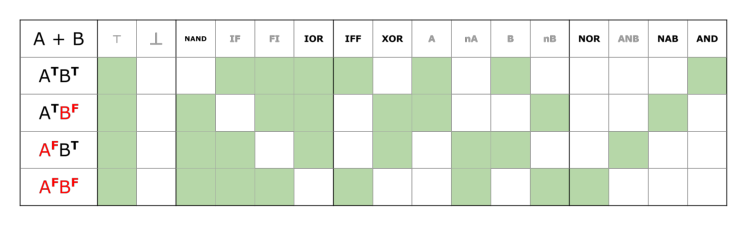
\includegraphics{figs/binaryLogicalConnectives-1} 

}

\caption{The truth table for the 16 binary logical connectives. The rows represent the set of situations where zero, one, or both propositions are true. The columns represent the 16 possible connectives and their truth conditions. Green cells represent true situations.}\label{fig:binaryLogicalConnectives}
\end{figure}
Logical systems often pick one or the other definition of disjunction
and give it more primacy. For example, Stoics considered exclusive
disjunction as primary. Inclusive disjunction was considered
``pseudo-disjunction'' or merely the negation of a conjunction. It seems
that the main reason for considering exclusive disjunction as primary
was that unlike inclusive disjunction, it cannot be concisely redefined
using conjunction and negation. Therefore, Stoics thought that exclusive
disjunction must have an independent and primary status as an operator
while inclusive disjunction is just a derivative. Unlike their Stoic
colleagues, medieval philosophers defined disjunction as inclusive.
Leibniz dispensed with both definitions of disjunction but later Bolzano
(1781-1840) used both. George Boole (1815 - 1864) gives more primacy to
exclusive disjunction since it corresponds to addition modulo 2. Later
Charles Sanders Peirce (1839-1914) changed Boole's system to use
inclusive disjunction instead. Inclusive disjunction has enjoyed a
primary role in modern logical systems since then.

The question of whether inclusive disjunction is ``primary'' in a
logical system or exclusive disjunction depends on the goal of the
system. The properties of exclusive disjunction make it ideal as an
operator for some purposes but not others. When it comes to natural
language semantics and modeling the meaning of the word \emph{or}, we
can similarly ask whether exclusive disjunction is primary (better
represents \emph{or}'s meaning) or inclusive disjunction. In the
following sections we will discuss linguistic work that has addressed
this issue but before I move to the discussion of disjunction in natural
language, I would like to comment on two properties of exclusive
disjunction that mismatch the properties of \emph{or} in English.

First the lack of idempotency suggests that the exclusive disjunction of
a proposition with itself (\(\phi or \phi\)) is necessarily false.
Applied to the word \emph{or} in natural languages, the prediction is
that a sentence such as ``Bob is happy or Bob is happy'' should be
judged as false regardless of whether Bob is happy or not. This
intuition seems to be absent in judgments of such sentences with
\emph{or}. In fact, there is an intuition that such disjunctions are
redundant and have the same truth value as the atomic proposition
itself. For example, ``the sky is blue or the sky is blue'' is redundant
and equivalent to ``the sky is blue''. This intuition is predicted if
\emph{or}'s meaning is represented by inclusive disjunction but not
exclusive disjunction.

Second, exclusive disjunction of two propositions has the same truth
values as the exclusive disjunction of their negatives
(\(\phi \oplus \psi \Leftrightarrow \lnot\phi \oplus \lnot\psi\)).
Considering the natural language \emph{or}, this property suggests that
the sentence ``the door is open or the window is open'' should have the
same truth conditions as ``the door is not open or the window is not
open''. However, the first seems false intuitively when both are closed
while the second is false when both are open. Therefore, two essential
properties of exclusive disjunction seem to mismatch the meaning of
\emph{or} in English. Inclusive disjunction on the other hand does not
face these problems. However, many examples of English \emph{or} such as
``He is a basketball player or a soccer player'' seem to exclude the
possibility of both disjuncts being true. Therefore, exclusive
disjunction seems to strong for the meaning of \emph{or} and inclusive
disjunction often falls short of the interpretation \emph{or} receives.
This tension has lead researchers in semantics and pragmatics to to
consider inclusive disjunction as the primary meaning of \emph{or} in
English, and resort to other mechanisms that pragmatically strengthen
the inclusive meaning of \emph{or} to exclusive or conjunctive
interpretations. In the next few sections, I briefly review the history
and the current issues in the semantics and pragmatics of disjunction.

\section{Disjunction in Language}\label{disjunction-in-language}

In natural languages, disjunction and conjunction are types of
coordination. Haspelmath (2007) defines coordination (or coordinate
constructions) as: ``syntactic constructions in which two or more units
of the same type are combined into a larger unit and still have the same
semantic relations with other surrounding elements.'' The example below
shows several coordinate constructions in English.
\begin{enumerate}
\def\labelenumi{(\arabic{enumi})}
\item
\end{enumerate}
\begin{enumerate}
\def\labelenumi{\alph{enumi}.}
\tightlist
\item
  The dog barked \emph{and} the cat ran behind the sofa.
\item
  I will get some coffee \emph{or} tea.
\item
  He went to bed \emph{because} he was sleepy.
\item
  She was sick \emph{but} she finished the homework.
\end{enumerate}
The word or affix that marks coordination is called a coordinator. The
coordinators are shown in italics in the example above. The units that
are marked by the coordinator are called coordinands. ``The dog barked''
is a coordinand in the first example. In English, a conjunction is a
coordination marked by the coordinator \emph{and} and a disjunction one
marked by \emph{or}. The coordinands in conjunctions and disjunctions
are called conjuncts and disjuncts respectively.

While there has been no report of a language that does not have ways to
express conjunction and disjunction, several languages lack overt
coordinators that mark conjunction or disjunction. In fact, Haspelmath
(2007) reports that the mere juxtaposition of the conjuncts is a
widespread strategy to convey conjunction crosslinguistically. For
disjunction, often the juxtaposition is also accompanied by a marker of
uncertainty or modality. For example, in Maricopa a sentence such as
``John and Bill will come'' is expressed as ``John, Bill, will-come.''
while the disjunction ``John or Bill will come'' is expressed as ``John,
Bill may-come.'' (Gil 1991) Similarly in Dyirbal a disjunction such as
``A or B'' is expressed as ``maybe A, maybe B'' (Dixon 1972: 363).
Similar effect of modals on the interpretation of coordination can also
be found in English. Consider the English examples below.
\begin{enumerate}
\def\labelenumi{(\arabic{enumi})}
\setcounter{enumi}{1}
\item
  Here is what you will see on the table: a book, a pen, a calculator.
\item
  Here is what you may see on the table: a book, a pen, a calculator.
\end{enumerate}
A list of items with no overt coordinator such as ``a book, a pen, a
calculator'' can be interpreted as a conjunction or a disjunction. In
the first sentence, the list is interpreted as a conjunction: you will
see a book, a pen, and a paper. In the second example, the list is
interpreted similar to a disjunction: you may see a book, a pen, or a
calculator. The sentences are identical except for the modal verbs. The
sentence with a disjunctive interpretation uses the possibility modal
\emph{may}. Ariel (2014) reports a similar naturally occurring example
with the modal \emph{perhaps}, repeated below. Such examples point to a
systematic connection between the notions of disjunction and modality.
\begin{enumerate}
\def\labelenumi{(\arabic{enumi})}
\setcounter{enumi}{3}
\item
  Practices of abortion, perhaps, pre-partum, perhaps postpartum (LSAC).
\item
  Practices of abortion, pre-partum, or postpartum.
\end{enumerate}
Languages that do mark coordination overtly do it in several ways. The
most common pattern, at lest in European languages, is to place the
coordinator in between the coordinands like ``A and B'' and ``A or B''
in English. However, other patterns such as ``A B-and'' where the
coordinator appears after the coordination is also attested (see
Haspelmath (2007) for more details). Another notable and common
cross-linguistic pattern is the doubling of the coordinator on each
coordinand. For example in Persian (Farsi), a disjunction can be
expressed using the disjunction word \emph{ya} like ``A ya B'' or it can
be doubled on each disjunct like ``ya A ya B''. Similar patterns have
been attested in Polish (``albo A albo B''), Dutch (``of A of B''),
Basque (``ala A ala B''), Somali (``ama A ama B''), and French (``ou A
ou B'') among many others. In English the \emph{either A or B}
construction comes close to this pattern. In the next section, I focus
on the interpretations of disjunction in English but the discussion is
not limited to English and similar results have also been attested in
other languages.

\section{Disjunction in English}\label{disjunction-in-english}

The use of the word \emph{or} in English is informally observed to
correlate with one or more of the following implications (Aloni, 2016):
\begin{enumerate}
\def\labelenumi{\arabic{enumi}.}
\tightlist
\item
  Inclusivity (IOR): at least one of the disjuncts is true;
\item
  Exclusivity (XOR): exactly one disjunct is true;
\item
  Conjunctivity (AND): both disjuncts are true;
\item
  Ignorance: the speaker does not know which disjunct is true;
\item
  Indifference: which disjunct is true does not matter for the purpose
  of the conversation.
\end{enumerate}
These five implications do not have equal status with respect to each
other. The first three (inclusivity, exclusivity, and conjunctivity) are
binary connective meanings discussed in section \ref{logic}. The fourth,
ignorance, is related to the knowledge state of the speaker, and the
fifth, indifference, is related to the role of disjunction within the
conversation.

These five implications are also not necessarily caused by the word
\emph{or} itself. They may directly stem from the meaning of \emph{or},
or they may be the result of \emph{or} interacting with several other
factors that shape the overall communicative message of the utterance.
The goal of semantic and pragmatic research on \emph{or} is to separate
the implication(s) contributed by \emph{or} from those caused by other
words or factors in the communication of meaning. Disentangling the
contribution of \emph{or} from the contribution of other communicative
elements has proven difficult, yet extremely fruitful in advancing
semantic and pragmatic theories. In what follows I try to provide a
short overview of the difficulties that \emph{or} poses to theories of
meaning.
\begin{longtable}[]{@{}lccccc@{}}
\caption{\label{tab:implications} Implications of \emph{or} for three
example sentences.}\tabularnewline
\toprule
\begin{minipage}[b]{0.45\columnwidth}\raggedright\strut
Example\strut
\end{minipage} & \begin{minipage}[b]{0.05\columnwidth}\centering\strut
IOR\strut
\end{minipage} & \begin{minipage}[b]{0.05\columnwidth}\centering\strut
XOR\strut
\end{minipage} & \begin{minipage}[b]{0.05\columnwidth}\centering\strut
AND\strut
\end{minipage} & \begin{minipage}[b]{0.12\columnwidth}\centering\strut
Ignorance\strut
\end{minipage} & \begin{minipage}[b]{0.12\columnwidth}\centering\strut
Indifference\strut
\end{minipage}\tabularnewline
\midrule
\endfirsthead
\toprule
\begin{minipage}[b]{0.45\columnwidth}\raggedright\strut
Example\strut
\end{minipage} & \begin{minipage}[b]{0.05\columnwidth}\centering\strut
IOR\strut
\end{minipage} & \begin{minipage}[b]{0.05\columnwidth}\centering\strut
XOR\strut
\end{minipage} & \begin{minipage}[b]{0.05\columnwidth}\centering\strut
AND\strut
\end{minipage} & \begin{minipage}[b]{0.12\columnwidth}\centering\strut
Ignorance\strut
\end{minipage} & \begin{minipage}[b]{0.12\columnwidth}\centering\strut
Indifference\strut
\end{minipage}\tabularnewline
\midrule
\endhead
\begin{minipage}[t]{0.45\columnwidth}\raggedright\strut
Study today or tomorrow, to pass the exam!\strut
\end{minipage} & \begin{minipage}[t]{0.05\columnwidth}\centering\strut
\(\checkmark\)\strut
\end{minipage} & \begin{minipage}[t]{0.05\columnwidth}\centering\strut
X\strut
\end{minipage} & \begin{minipage}[t]{0.05\columnwidth}\centering\strut
X\strut
\end{minipage} & \begin{minipage}[t]{0.12\columnwidth}\centering\strut
\(\checkmark\)\strut
\end{minipage} & \begin{minipage}[t]{0.12\columnwidth}\centering\strut
\(\checkmark\)\strut
\end{minipage}\tabularnewline
\begin{minipage}[t]{0.45\columnwidth}\raggedright\strut
Bob studied yesterday or the day before.\strut
\end{minipage} & \begin{minipage}[t]{0.05\columnwidth}\centering\strut
X\strut
\end{minipage} & \begin{minipage}[t]{0.05\columnwidth}\centering\strut
\(\checkmark\)\strut
\end{minipage} & \begin{minipage}[t]{0.05\columnwidth}\centering\strut
X\strut
\end{minipage} & \begin{minipage}[t]{0.12\columnwidth}\centering\strut
\(\checkmark\)\strut
\end{minipage} & \begin{minipage}[t]{0.12\columnwidth}\centering\strut
X\strut
\end{minipage}\tabularnewline
\begin{minipage}[t]{0.45\columnwidth}\raggedright\strut
Students, like Bob or Becky, will pass.\strut
\end{minipage} & \begin{minipage}[t]{0.05\columnwidth}\centering\strut
X\strut
\end{minipage} & \begin{minipage}[t]{0.05\columnwidth}\centering\strut
X\strut
\end{minipage} & \begin{minipage}[t]{0.05\columnwidth}\centering\strut
\(\checkmark\)\strut
\end{minipage} & \begin{minipage}[t]{0.12\columnwidth}\centering\strut
X\strut
\end{minipage} & \begin{minipage}[t]{0.12\columnwidth}\centering\strut
X\strut
\end{minipage}\tabularnewline
\bottomrule
\end{longtable}
Table \ref{tab:implications} shows three example sentences with the
disjunction word \emph{or} and marks the presence or absence of each
\emph{or}-implication. A sentence such as ``Study today or tomorrow, to
pass the exam.'' implies that the addressee is asked to study today,
tomorrow, or possibly both days. The overall message is that the
addressee should study at least one of those two days to pass the exam.
It does not rule out the possibility of the addressee studying both
today and tomorrow, so there is no exclusivity implication. Furthermore,
it is not asking the addressee to both ``study today'' \textbf{and}
``study tomorrow'', so a conjunctive implication is absent. It is also
possible to infer that the speaker does not know or it does not matter
to them whether the addressee studies today or tomorrow. The command is
complied with as long as the addressee studies one of those two days.
Compare this to a sentence like ``Bob studied yesterday or the day
before.'' The overall message is that Bob studied one day and that day
may have been yesterday or the day before. It suggests that Bob did not
study both yesterday and the day before, so there is an exclusivity
implication and no conjunctivity implication. It is also implied that
the speaker does not know which day exactly Bob studied so we have an
ignorance implication, but it is not implied that the speaker is
indifferent towards which day Bob actually studied. Now compare the
previous sentences to a sentence such as ``students like Bob or Becky
will pass the exam.'' This sentence does not imply inclusivity or
exclusivity. It does not communicate anything like ``Either students
like Bob will pass, or students like Becky will pass, or both.'' It does
not exclude the possibility of students like both Bob and Becky passing
at all. In fact to the contrary, the main message is that ``both
students like Becky \textbf{and} students like Bob will pass''. In this
example, \emph{or} has a conjunctive implication. Even replacing
\emph{or} with \emph{and} does not substantially alter the meaning of
the sentence: ``students like Bob and Becky will pass the exam''. No
ignorance or indifference implication accompanies this conjunctive
implication.

Just looking at Table \ref{tab:implications} one might conclude that
there is no systematicity behind the use of \emph{or} and the
implications that accompany it. This was indeed the prevailing view
among many logicians and philosophers that considered language messy,
fraught with ambiguities, and illogical. For example, while discussing
disjunction in his influential introductory book on logic, Alfred Tarski
warns readers about the many interpretations of \emph{or} in natural
language and explains that there are ``quite noticeable differences
between the usage of it in everyday language and in logic.''(Tarski,
1941). He first points out that ``the word \emph{or} in everyday
language has at least two different meanings''. A child may ask us to be
taken to a hike in the morning and a theater in the afternoon, but we
may respond: ``No, we are going on a hike or we are going to the
theater''. He explains that the interpretation of \emph{or} in this
example is exclusive because ``we intend to comply with only one of the
two requests'' and not both. However, a disjunction may also have an
inclusive interpretation like the following example: ``Customers who are
teachers or college students are entitled to a special reduction''.
Tarski explains that \emph{or} in this example is inclusive ``since it
is not intended to refuse reduction to a teacher who is at the same time
a college student.'' He advises readers to avoid this exclusive
vs.~inclusive ambiguity by reserving the word \emph{or} for the
``logical'' (inclusive) sense and use the construction ``either \ldots{}
or \ldots{}'' for the exclusive one.

However, he immediately notes that there are other interpretations of
\emph{or} that go beyond the exclusive/inclusive distinction. I include
his discussion here directly since in addition to addressing the
ignorance implication of \emph{or}, it foreshadows future developments
in semantics and pragmatics initiated years later by Paul Grice.
\begin{quote}
``In commmon language, two sentences are joined by the word \emph{or}
only when they are in some way connected in form and content. (The same
applies, though perhaps to a lesser degree, to the usage of the word
\emph{and}) \ldots{} anybody unfamiliar with the language of
contemporary logic would presumably be little inclined to consider such
a phrase as''2+2=5 or New York is a large city" as a meaningful
expression, and even less so to accept it as a true sentence. Moreoever,
the usage of the word \emph{or} in everyday English is influenced by
certain factors of a psychological character. Usually we affirm a
disjunction of two sentences only if we believe that one of them is true
but wonder which one. If, for example, we look upon a lawn in normal
light, it will not enter our mind to say that the lawn is green or blue,
since we are able to affirm something simpler, and at the same time,
stronger, namely that the lawn is green. Sometimes even, we take the
utterance of a disjunction as an admission by the speaker that he does
not know which of the members of the disjunction is true. And if we
later arrive at the conviction that he knew at the time that one -- and
specifically, which -- of the members was false, we are inclined to look
upon the whole disjunction as a false sentence, even should the other
member be undoutedly true. Let us imagine, for instance, that a friend
of ours, upon being asked when he is leaving town, answers that he is
going to do so today, tomorrow, or the day after. Should we then later
assertain that, at that time, he had already decided to leave the same
day, we shall probably get the impression that we were delibrately
misled and that he told us a lie. The creators of contemporary logic,
when introducing the word \emph{or} into their considerations, desired,
perhaps unconsciously, to simplify its meaning and to render the latter
clearer and independent of psychological factors."
\end{quote}
Tarski ended his discussion by saying that these linguistic and
psychological factors should not enter logical considerations. The view
that language is not amenable to the tools of logic remained prevalent
but faced substantial challenges from philosophers that argued for more
attention to ordinary language use. Finally, the work of two
philosophers, Richard Montague, a student of Tarski, and Paul Grice,
tilted arguments towards the ``ordinary language'' philosophers.
Montague's focus was on quantification in logic and natural language
while Grice focused on the logical connectives such as \emph{or} and
\emph{if}. Grice (1989) argued that the perceived differences between
the meaning of natural language words such as \emph{or} and the
operators in formal logic such as inclusive disjunction ``arise from
inadequate attention to the nature and importance of the conditions
governing conversation.'' He set out to show that when we take
conversational factors into account, the meaning of linguistic
connectives are similar to the common definitions of their counterparts
in formal logic.

An important contribution of Grice was his typology of meaning that lead
to the establishment of semantics and pragmatics. He differentiated
between ``what is said'' and ``what is implied''. ``What is said''
refers to the literal meanings of words; the conventional association
between words and meanings that is independent of any particular
context. ``What is said'' is the most primary type of meaning and not
derived from any other process. The field of semantics is concerned with
this type of meaning and all else that relies on context of use is
relegated to pragmatics. On the other hand, ``what is implied''
(conversationally) or as he called them ``conversational implicatures''
refer to meanings that are created by using words and sentences in
specific contexts\footnote{I set aside conventional implicatures here
  since they do not come up in the semantics and pragmatics of
  disjunction.}. Conversational implicatures are the result of refining
the literal meanings of words (what was said) to suit the assumptions
and purposes of the conversational context. As such, implicatures are
derivative and not primary.

Grice was also influential because he pioneered the methodology of
studying linguistic meaning. He viewed the interpretation of an
utterance as the composite of many interacting factors. In order to
understand the literal meaning of a word, a semanticist needs to examine
it in different contexts and understand its interaction with other
factors that shape the general interpretation of the utterance.
Utterances containing a word like \emph{or} may be interpreted
differently in different contexts, giving the impression that the word
is polysemous. However, it is possible that the word has one underlying
meaning (i.e.~its semantics) and that in interaction with other elements
of the sentence and the conversation, it gives rise to a variety of
interpretations. In such cases, the underlying meaning can be recovered
by detecting the factors that influence interpretation and reversing
their effects. In Grice's view, true polysemy is stable polysemy across
a wide range of contexts.

In addition to context-sensitivity, Grice suggested cancellability and
computability as other properties of pragmatic enrichment.
Cancellability refers to the following observation: a speaker explicitly
denying a pragmatic enrichment of what they said does not result in the
speaker contradicting themselves. For example, if I say that ``the
chocolate box is in the fridge or the cupboard'', you may infer that I
do not know where it is (ignorance implication). But, I can continue by
saying ``I know where it is but I'm not going to tell you'' without
contradicting what I said before. According to Grice, this suggests that
the ignorance implication is not part of the literal meaning of what I
said. The idea is that my continuation cancelled the pragmatic inference
that I do not know where the chocolate box is. With literal meaning on
the other hand, a speaker explicitly denying what they literally said
results in a contradiction. For example, if I say ``the chocolate box is
in the fridge or the cupboard'', I cannot add ``it is in neither place''
without sounding contradictory. Grice also emphasized on calculability
of non-literal (non-conventional) meaning (i.e.~conversational
implicatures). He believed that if researchers propose a certain
interpretation to be non-literal (more accurately non-conventional),
they should be able to explain the mechanism that gave rise to that
interpretation. Finally, it is important to note that Grice did not mean
to introduce an exhaustive and definite set of diagnostics to
distinguish literal and implicated meaning. He emphasized that in many
cases, our intuitions will be the guide on what is said literally and
what is merely implicated by what is said.

\section{Factors Involved in the Interpretation of
Disjunction}\label{factors-involved-in-the-interpretation-of-disjunction}

This section presents a brief list of factors that influence the
interpretation of disjunction in English. This list is not meant to be
exhaustive; it only provides a window into the factors that an account
of disjunction acquisition needs to consider. The factors discussed in
this section include: conversational principles, entailment environment,
modality, semantics of the disjuncts, metalinguistic communication
(definitions and repairs), syntactic categories of the disjuncts,
question intonation, embedded imperatives, and alternative unconditional
constructions. I start this section with Grice's discussion of
conversational principles that contribute to the overall interpretation
of an utterance.

\subsection{Conversational Principles}\label{conversational-principles}

Grice's focus was on how conversational factors enrich utterance
interpretation. He saw conversation as a cooperative social activity in
which participants follow a certain set of rules or ``maxims''. Below I
list the overarching ``cooperative principle'' as well as its maxims.
Grice contended that these maxims further enrich the primary meaning of
words and sentences in a given context. He used the term
\emph{conversational implicature} to refer to implications that are
derived from the cooperative principle and the conversational maxims.
\begin{itemize}
\tightlist
\item
  \textbf{Cooperative Principle}: Make your conversational contribution
  such as is required, at the stage at which it occurs, by the accepted
  purpose or direction of the talk exchange in which you are engaged.
  \begin{itemize}
  \tightlist
  \item
    \textbf{Maxim of Quality}: Try to make your contribution one that is
    true. Do not say what you believe to be false. Do not say that for
    which you lack adequate evidence. things for which you lack
    evidence.
  \item
    \textbf{Maxim of Quantity}: Make your contribution as informative as
    required. Do not make your contribution more informative than is
    required.
  \item
    \textbf{Maxim of Relation}: Be relevant.
  \item
    \textbf{Maxim of Manner}: Be perspicuous. Avoid obscurity of
    expression. Avoid ambiguity. Be brief. Be orderly.
  \end{itemize}
\end{itemize}
Grice's account provided some informal explanations for the divergences
between the interpretation of \emph{or} and inclusive disjunction in
logic. For example, Tarski pointed out that sentences that are connected
with \emph{or} should be related with respect to their content. He
reported that English speakers find a sentence like ``2+2=5 or New York
is a large city'' very odd and hard to judge as true, even though one of
the disjuncts is certainly true. Grice's ``maxim of relation'' provides
an independently motivated explanation for this observation. In
conversations, speakers are expected to provide relevant information to
the topic of the conversation. It is extremely hard to think of a
context where ``2+2=5'' and ``New York is a large city'' are relevant
alternatives to the conversational topic. Tarski himself noticed,
however, that this phenomenon is not limited to the word \emph{or}.
Other connectives face the similar problem: ``2+2=4 and New York is a
large city'' or ``if 2+2=4, then New York is a large city''.

Tarski also pointed out that a disjunction such as ``A or B'' is often
odd when the speaker knows which alternative is true. In other words, a
disjunction often implies that the speaker is ignorant with respect to
the truth of the disjuncts. The definition of disjunction in classical
logic lacks this aspect. Grice's theory provides a separate mechanism
that is responsible for the ignorance implication. The maxim of quality
requires the speaker to say what they believe to be true and the maxim
of quantity requires them to be as informative as required. In many
contexts the speaker is expected to be maximally informative. If the
speaker knows A then they should say ``A''. In Tarski's example, if the
speaker knows that the grass is green, then the most informative
statement would be ``the grass is green.'' Saying that ``the grass is
green or blue'' goes against the maxim of quantity. The speaker is
providing less information even though it is clear they know more.
However, as Grice points out, in some contexts there is a reason for
being underinformative and in such cases there is no ignorance
implication. For example, he mentions that in a treasure hunt with his
children, he may say: ``The prize is in the garden or the attic. I know
that because I know where I put it, but I'm not going to tell you.'' In
this context the speaker knows which alternative is true. However, the
context does not require him to be maximally informative. In fact, given
the rules of a treasure hunt, he is required to not divulge the
whereabouts of the prize. Therefore, the speaker's underinfomative
utterance is warranted. This way Grice shows that the ignorance
implication is not part of what \emph{or} means but rather the result of
\emph{or} interacting with conversational maxims. It is important to
point out that a disjunction such as ``A \emph{or} B'' is unacceptable
when conversational participants already know which disjunct is true. In
Grice's example, while Grice knows which disjunct is true (there is no
speaker ignorance), the addressee does not. However, in Tarski's
example, both the speaker and the addressee know whether the grass is
green or blue.

Tarski discussed the exclusive and inclusive interpretations of
\emph{or} as well. He explained that even though in logic a disjunction
is commonly defined as inclusive, a sentence like ``we are going on a
hike or we are going to the theater'' has an exclusive interpretation.
Grice's account provides an explanation for this supposed ``ambiguity''
as well. In some contexts, the speaker knows whether both alternatives
are true or not (Competence Assumption). If the speaker knows both
alternatives to be true and the context requires maximal
informativeness, then they should use the connective \emph{and}. If they
know that only one alternative is true, then they cannot use \emph{and}
because using it would violate quality (the speaker has said something
false.) In such contexts using \emph{or} instead of \emph{and} implies
that only one alternative is true and not both. The exclusive example
provided by Tarski is similar to such contexts. The father knows (and in
fact decides) whether both alternatives will be true or only one. If he
intended for both to be true he could use the word \emph{and}: ``we are
going on a hike and we are going to the theater''. Since he did not, we
can infer that he does not intend to do both. In fact in Tarski's
original context, the father says the sentence with \emph{or} in
contrast to the child's utterance with \emph{and}.

The Gricean account has been developed and made more explicit by several
authors. Here I present the current standard neo-Gricean account which
is mostly due to U. Sauerland (2004). Assuming the speaker has uttered a
disjunctive assertion such as ``P or Q'', the reasoning proceeds as
follows:
\begin{itemize}
\tightlist
\item
  \textbf{Utterance}: the speaker said ``P or Q''.
\item
  \textbf{Alternatives}: the speaker could have said: P, Q, or ``P and
  Q''. Why didn't s/he?
  \begin{enumerate}
  \def\labelenumi{\arabic{enumi}.}
  \tightlist
  \item
    \textbf{Ignorance}: The speaker is uncertain about the truth of P
    (i.e. \(\lnot B_S (P)\))
  \item
    \textbf{Ignorance}:The speaker is uncertain about the truth of Q
    (i.e. \(\lnot B_S (Q)\))
  \item
    \textbf{Ignorance}: The speaker is uncertain about the truth of P
    and Q (i.e. \(\lnot B_S (P \land Q)\))
  \end{enumerate}
\item
  \textbf{Comeptence}: The speaker knows whether both propositions hold
  or not (i.e. \(B_S (P \land Q) \lor B_S \lnot (P \land Q)\))
  \begin{enumerate}
  \def\labelenumi{\arabic{enumi}.}
  \setcounter{enumi}{3}
  \tightlist
  \item
    \textbf{Exclusivity}: Given ignorance inference 3 and speaker
    competence, the speaker believes that only one of the disjuncts is
    true (i.e. \(B_S \lnot (P \land Q)\)).
  \end{enumerate}
\end{itemize}
Inferences 1-3 are ignorance implications. It is important to notice
that the exclusivity inference in step 4 develops from the ignorance
inference in step 3 and the the competence assumption. For the
exclusivity implicature to arise, the context of the utterance must be
one where the speaker should know whether both disjuncts hold or not,
but s/he is not sure about which one holds. As Geurts (2006) argues, it
is not clear how common such contexts are and what proportion of
exclusivity implications are in fact implicatures derived via this type
of pragmatic reasoning. Nevertheless, it is not impossible to think of
such contexts. For example, if I say that ``Bob went to the shop and
bought a cardigan or a shirt'', it is reasonable for the addressee to
assume that I know whether one item was bought or two. At issue is not
whether exclusivity implicatures exist at all but rather how common are
they. The semantics and pragmatics literature seems to have an
assumption that at least the majority of exclusivity implications are
derived via the Gricean reasoning sketched above.

While ignorance, indifference, and exclusivity implications of \emph{or}
can be explained (at least partly) via the Gricean mechanism above, the
conjunctive interpretation remains unexplained. Geurts (2010) revises
the Gricean account to cover the conjunctive inferences of free-choice
expressions like ``you can have coffee or tea''. Potts \& Levy (2015)
extend the Gricean account to cover definitional uses like ``he is a
wine lover or an oenophile''. I will discuss free-choice inferences and
definitional uses below. As far as I know, there are no Gricean accounts
for conjunctive interpretations of discussion for sentences that provide
examples such as ``Students, like Bob or Becky, will pass.'' There are
also no Gricean accounts for examples of self-repair with disjunction
such as ``Bob changed the font, or I mean, the size of the text.'' These
cases will be discussed below as well.

Before moving on, I would like to add that in Gricean pragmatics, the
notion of ``alternatives'' or ``what the speaker could have said'' plays
a crucial role. In case of the ignorance implicature, the explanation
relies on the assumption that instead of ``A or B'' the speaker could
have said something simpler but more informative, namely ``A''. The
Gricean explanation relies on the addressee reasoning about why the
speaker did not just say ``A''. In case of the exclusivity implication,
the Gricean approach relies on the assumption that instead of ``A or B''
the speaker could have used a different connective, namely \emph{and} to
say ``A and B''. The addressee reasoning about why the speaker did not
do so derives the exclusivity implicature. Alternatives also play an
important role in developmental accounts of pragmatics. Barner, Brooks,
\& Bale (2011) argue that children are not adult-like in their access to
the linguistic alternatives and as a result, they show non-adult-like
pragmatic inferences.

An active area of research in Gricean pragmatics is the question of what
constitutes an alternative and how implicatures are computed given a set
of alternatives to the asserted utterance. The alternatives to a lexical
item were traditionally considered as a scale ordered by entailment. L.
R. Horn (1972) proposed that words such as \emph{or} and \emph{and} as
well as \emph{some} and \emph{all} form scales of alternatives
represented as \textless{}\emph{or}, \emph{and}\textgreater{} and
\textless{}\emph{some}, \emph{many}, \emph{most},
\emph{all}\textgreater{}. This is why the exclusivity implicature of
\emph{or} is also called a ``scalar implicature''. The basic idea is
that asserting an utterance with the weaker lexical item on the scale
(e.g. \emph{or}) results on the inference that the corresponding
utterance with the the stronger item (e.g. \emph{and}) would have been
false (violated the maxim of quality). However, using the scale
\textless{}\emph{or}, \emph{and}\textgreater{} will only derive the
exclusivity implicature and does not provide an account of ignorance
implications. In the standard account provided above, the ignorance
implications rely on including each disjunct in the alternative set as
well. Due to this problem (among others), the notion of ``scale'' has
been replaced by ``the set of alternatives''. Nevertheless the term
``scalar implicature'' is still used to refer to the implicatures of
\emph{some}, and \emph{or}. A large body of literature suggests that
children do not compute scalar implicatures at the rate that adults do.
I discuss this issue more in the next two chapters.

\subsection{Entailment Environment}\label{entailment-environment}

The concept of ``entailment'' plays an important role in logic and
semantics. The concept is often introduced as a relation among
propositions such that \(P\) entail \(Q\) if and only if \(P\) being
true necessarily makes \(Q\) true. Based on this, two other notions are
defined: upward entailing environment and downward entailing
environments.
\begin{itemize}
\item
  A linguistic environment \(\phi\) is upward entailing if and only if
  for any two expressions \(a\) and \(b\), if \(a\) entails \(b\), then
  \(\phi[a]\) entail \(\phi[b]\).
\item
  A linguistic environment \(\psi\) is downward entailing if and only if
  for any two expressions \(a\) and \(b\), if \(a\) entail \(b\), then
  \(\psi[b]\) entail \(\psi[a]\).
\end{itemize}
Let's consider \(a\) as ``student'', \(b\) as ``human'', \(\phi\) as
``Roxy is a {[}{]}'', and \(\psi\) as ``Roxy isn't a {[}{]}''. Since
``student'' entails ``human'', and ``Roxy is a student'' entails ``Roxy
is a human'', we can conclude that ``Roxy is a {[}{]}'' is an upward
entailing environment. On the other hand, ``student'' entails ``human''
but ``Roxy isn't a human'' entail ``Roxy isn't a student''. Therefore,
we can conclude that ``Roxy isn't a {[}{]}'' is a downward entailing
environment. In short, upward entailing environments preserve entailment
direction while downward entailing environments reverse it.

As explained earlier, exclusive disjunction entails inclusive
disjunction. In an upward entailing environment, this entailment
relation is preserved: ``Roxy is a student or a teacher (but not both)''
entails ``Roxy is a student or a teacher (or both).'' However, in a
downward entailing environment this relation is reversed: ``Roxy isn't a
student or a teacher (neither)'' entails ``Roxy isn't a student or a
teacher (but may be both or neither)'' A common observation is that the
exclusive interpretation of \emph{or} is more common in upward entailing
environments while the inclusive interpretation is more common in
downward entailing environments. For example a disjunction like ``he is
a student or a teacher'' is more likely to be interpreted as
``exclusive'' while its negative counterpart ``not a student or a
teacher'' is more often interpreted as ``neither'', which is expected if
\emph{or} is inclusive. This is predicted by Grice's maxim of quantity.
In an upward entailing environment, exclusive disjunction is stronger
and conveys more information. In a downward entailing environment, this
pattern is reversed; inclusive disjunction results in a stronger and
more informative statement. If a listener expects the speaker to make
their contribution as informative as possible, then we can expect a bias
towards exclusive disjunction in upward entailing environments and
inclusive disjunction in downward entailing ones.

As explained in the section on logic and disjunction, the interaction of
negation with disjunction, and conjunction is captured by the so-called
De Morgan laws repeated below. We can generalize from negation to all
downward entailing environments and re-write the De Morgan laws with
\(\Delta\) representing a downward entailing environment.
\begin{itemize}
\tightlist
\item
  Generalized De Morgan's Laws:
  \begin{itemize}
  \tightlist
  \item
    \(\Delta (\phi \lor \psi) \Leftrightarrow \Delta \phi \land \Delta \psi\)
  \item
    \(\Delta (\phi \land \psi) \Leftrightarrow \Delta \phi \lor \Delta \psi\)
  \end{itemize}
\end{itemize}
It is sometimes argued that the interaction of downward entailing
environments with disjunction and conjunction follow these rules in
natural language. For disjunction the argument is that (not A or B) is
interpreted as the conjunction of negatives (not A and not B). While
this may be true in many and perhaps majority of cases, there are
notable and systematic exceptions. This point is perhaps best
illustrated by the negative phrase ``not one or the other'' in the
following naturally occurring examples (5-9). In (5) below, ``not one or
the other'' is used to mean ``both''. In example (6) it is used to mean
``neither''. In the (7) and (8) examples, the authors explicitly explain
that by ``not one or the other'' they mean ``neither or both''. Finally
(9) shows that these observations are not isolated to the expression
``one or the other''.
\begin{enumerate}
\def\labelenumi{(\arabic{enumi})}
\setcounter{enumi}{5}
\item
  Speed or Quality? It's Not One or the Other. It's Both! (Online
  Blogpost title by Chris Manuel)
\item
  There is no in‑between: you're either masculine or feminine because
  you're either male or female, and if you're not one or the other of
  these two genders, then there must by something wrong with you. In
  numerous other cultures, however, there are gender systems that are
  not binary.
\item
  In the above example {[}containing this expression: \$time
  =\textasciitilde{} /(\d+):(\d+)(:(\d+))?/{]}, the third set of
  parentheses is used to associate both the colon and the digits with
  ``?'' - either both should be specified, or neither, but not one or
  the other. (Response to a programming exercise on an online forum)
\item
  Everything is either physical or spiritual \ldots{} This is of course
  the root of the problem \ldots{} If things are either A or B, it
  actually makes sense to assume that once they're not one, then they
  are the other. But what if they're not A or B? what if, for instance,
  they're neither? Or \ldots{} both? (Medium Article by Doc Ayomide: I'm
  Christian and I don't believe mental illness is spritiual)
\item
  The church of the Lord is not here or there, but everywhere. (online
  newsletter at newchurch.org)
\end{enumerate}
The examples above suggest that in natural language, the negation of a
disjunction is not necessarily the conjunction of negations. These
examples are not presented here to suggest that the NOR and AND
interpretations of not (A or B) are equally likely. The examples show
the importance of linguistic and non-linguistic factors in shifting our
biases one way or another. Entailment environment is simply one of these
factors.

Nevertheless, research in semantics has shown that entailment
environment is an important factor in the interpretation and
distribution of lexical items (see Giannakidou (2011) for a discussion).
Based on this, Crain (2012) has suggested that the entailment
environment and its interactions with logical words such as \emph{or}
must be an innate property of the human mind. I will cover this nativist
model of logical word acquisition in the next chapter. In the next
section I discuss the role of modality in the interpretation of
disjunction.

\subsection{Modals}\label{modals}

The interaction of \emph{or} with modals, especially possibility modals
such as \emph{may} and \emph{can} presented the biggest challenge for
the proposal that \emph{or} has the semantics of inclusive disjunction.
The issue was first discussed by Kamp (1973) in the context of giving
permissions. Consider a sentence like: ``You may pay using cash or
credit card.'' It has two main interpretations. One is the standard
inclusive interpretation which is more accessible if it is followed by
an expression of uncertainty: ``you may use cash or you may use credit
card, or possibly both but I'm not sure''. This interpretation is
predicted by the standard inclusive account. However, there is a second
and often more prominent interpretation for this sentence which suggests
customers are free to choose: they are allowed to use cash \emph{and}
they are allowed to use credit card. This so called ``free choice''
interpretation is not expected if \emph{or} means inclusive disjunction
and \emph{may} acts like a standard possibility modal. ``It is possible
that A or it is possible that B'' weaker and less informative than ``it
is possible that A and it is possible that B''. However, it seems that
in natural language when \emph{or} appears with possibility modals it
can have both interpretations. There have been many proposals to tackle
this problem. Here I discuss two main proposals and expand on one that
has made its way into acquisition research. In one approach,
semanticists abandoned the truth-conditional inclusive semantics of
\emph{or} and proposed that \emph{or} encodes the conjunction of two
possibilities (Geurts, 2005; Zimmermann, 2000). In a second approach,
they kept the standard semantics of \emph{or} and treated the free
choice inference as an implicature (Fox, 2007; Geurts, 2010).

First, Zimmermann (2000) made a departure from the truth-functional
account of \emph{or} and proposed that \emph{or}'s meaning is inherently
modal. ``A or B'' expresses the conjunction of two possibilities and can
be paraphrased as ``It is possible that A and it is possible that B,''
represented in modal logic as \(\Diamond A \land \Diamond B\). For
example, ``Bob paid using cash or credit card'' is equivalent to ``It is
possible that Bob paid using cash and it is possible that Bob paid using
credit card.'' The modal account of \emph{or} predicts a different
logical structure for the free choice sentences. A sentence like ``Bob
is allowed to pay using cash or credit card'' will have two layers of
possibility modals: \(\Diamond\Diamond A \land \Diamond\Diamond B\),
roughly paraphrased as ``it is possible that Bob is allowed to pay using
cash and it is possible that Bob is allowed to pay using credit card.''
This is the interpretation without a free-choice implication. The
free-choice interpretation is only derived when the speaker is assumed
to be an ``authority'' on the subject. According to the ``authority
principle'', if an authority considers it possible that Bob is allowed
to pay in cash, then Bob is allowed to pay in cash
(\(\Diamond \Diamond A \rightarrow \Diamond A\)). Assuming speaker
authority, a statement like ``it is possible that Bob is allowed to pay
using cash and it is possible that Bob is allowed to pay using credit
card'' reduces to ``Bob is allowed to pay using cash and Bob is allowed
to pay using credit card''
(\(\Diamond\Diamond A \land \Diamond\Diamond B \rightarrow \Diamond A \land \Diamond B\)).
Therefore, the modal account of disjunction provides a straightforward
answer to the puzzle of free-choice interpretations, yet it dispenses
with the truth-functional account of disjunction.

The pragmatic approach strives to keep the truth-functional meaning of
\emph{or} and analyze the free-choice interpretation as an implicature.
It takes two observations as its starting point. First, that the
free-choice inference is cancellable. As explained before, ``you are
allowed to drink tea or coffee'' can be followed with ``but I'm not sure
which'', therefore not implying that the addressee has free choice
between tea and coffee. Second, when we add negation to free-choice
sentences, the interpretation is not the negative of the conjunctive
free-choice interpretation, but rather the negative of the standard
account in which disjunction is inclusive. For example, the main
interpretation of a sentence like ``you are not allowed to drink tea or
coffee'' is one where neither option is allowed. This interpretation is
expected if negation is operating on the possibility modal and an
inclusive disjunction (\(\lnot \Diamond (A \lor B)\)). Proponents of the
pragmatic approach argue that this behavior is not limited to negation
and applies to downward entailing environments more generally. Consider
a sentence like: if I'm allowed to drink tea or coffee, I'll be happy.
We can infer that the speaker will be happy even if they are only
allowed to drink tea. However, under a conjunctive interpretation of
\emph{or} with \emph{allowed to}, one should expect that the speaker
will only be happy if both are allowed. This is not the interpretation
we intuit. The pragmatic approach keeps the semantics of \emph{or} as
inclusive disjunction and contends that similar mechanisms should
explain exclusivity as well as conjunctive (free-choice) implication.
(Chierchia, 2013; Fox, 2007; Geurts, 2010) In what follows I sketch Fox
(2007)'s analysis of free-choice inferences of \emph{or} which was later
adopted by Singh, Wexler, Astle-Rahim, Kamawar, \& Fox (2016) to explain
why children sometimes appear to interpret disjunction similar to
conjunction in simple declaratives.

Applying the ordinary pragmatic mechanism explained earlier to sentences
with modals such as \emph{may} and \emph{allowed to} results in the
wrong prediction. The problem lies in the alternatives considered for
pragmatic computation. Consider the sentence ``you are allowed to drink
coffee or tea''. The standard alternatives to this sentence are: you are
allowed to drink coffee, you are allowed to drink tea, and you are
allowed to drink coffee and tea. If we mechanistically apply the Gricean
recipe, we derive nothing more than the standard interpretation: ``you
are allowed to drink coffee or tea; but the speaker is not certain that
you are allowed to drink coffee, and the speaker is not certain that you
are allowed to drink tea, and the speaker is not certain that you are
allowed to drink both coffee and tea''. This is not the free-choice
inference we have been looking for.

Fox (2007) resolves this issue by changing the alternatives. As
explained before, the standard set of alternatives to a disjunction like
``A or B'' is A, B, and ``A and B''. For the sentence ``you are allowed
to drink coffee or tea'', the standard alternatives are ``you are
allowed to drink coffee'' (\(\Diamond A\)), ``you are allowed to drink
tea'' (\(\Diamond B\)), and ``you are allowed to drink coffee and tea''
(\(\Diamond A \land \Diamond B\)). Fox (2007) proposes that the
alternatives are instead the following set: ``you are only allowed to
drink coffee'' (\(\Diamond A \land \lnot \Diamond B\)), ``you are only
allowed to drink tea'' (\(\Diamond B \land \lnot \Diamond A\)``),
and''you are allowed to drink coffee and tea"
(\(\Diamond A \land \Diamond B\)). What justifies the change of
alternatives from ``allowed to X'' to ``only allowed to X''? In Fox
(2007)'s system this follows from the syntactic structure of these
sentences. They contain a silent operator that has similar semantic
effects as the word \emph{only}. The process of applying this operator
to a linguistic expression is called ``exhaustification'', and the
operator is commonly abbreviated as EXH. In short, EXH(\(\phi\)) asserts
that \(\phi\) is true and every alternative not entailed by \(\phi\) is
false. In Fox (2007)'s account, EXH applies to each disjunct, as well as
the disjunction as a whole. The final product is the following
implication: ``you are allowed to drink coffee or tea; not \textbf{only}
coffee, not \textbf{only} tea, and not both coffee and tea.''

Geurts (2010) uses essentially the same solution as that of Fox (2007),
but casts it in a pragmatic framework rather than a syntactic one. He
suggests that pragmatic reasoning is intention based and even though
linguistic alternatives are important, it the set of possible
communicative intentions that play the key role in pragmatic
computation. When a sentence such as ``you are allowed to drink coffee
or tea'' is uttered, the listener considers four possible communicative
intentions: (1) coffee and tea are both allowed, (2) coffee is allowed
but tea isn't,(3) tea is allowed but coffee isn't, and (4) neither is
allowed. He explains that intention (4) is ruled out because it is in
contradiction with the basic meaning of the utterance. Options (2) and
(3) are ruled out because if the speaker meant to convey them, they
could have said something simpler, namely ``you are allowed to drink
tea'' or ``you are allowed to drink coffee''. The only intention left
that satisfies Gricean maxims is intention (1) which is the desired
free-choice inference.

While the literature on the interaction of disjunction with modals has
mostly focused on possibility modals such as \emph{may} and the context
of giving permissions, similar conjunctive inferences are present with
preference/desire modals such as \emph{want}, \emph{like}, and
\emph{love}. If we say ``Bob likes/loves going on hikes or climbing
rocks or staying outdoors'', it is clear that Bob likes all the
activities listed. Therefore, it is possible to infer that ``Bob
likes/loves rock climbing.'' Similarly, we can infer from ``Bob would
like some coffee or tea'' that ``Bob \textbf{would like} some coffee''
and ``Bob \textbf{would like} some tea'' (The inference is easier to
access when \emph{would like} is stressed). Similar inferences seem to
be valid for ``Bob wants some coffee or tea.'' However, it seems that
the conjunctive inferences in such cases are not as strong as the case
of permissions like ``Bob is allowed to drink coffee or tea.'' Perhaps
the strongest case of conjunctive inferences comes in the context of
providing examples with the word ``like''. In a sentence such as
``Students like Bob or Becky never fail'', the disjunction word is
almost equivalent to a conjunction: ``Students like Bob and Becky never
fail.'' These observations suggests that \emph{or} receives conjunctive
interpretations in a wider range of environments than commonly discussed
in the literature.

\subsection{Disjunct Semantics}\label{disjunct-semantics}

Geurts (2006) points out that even though pragmatic reasoning may be the
reason behind some exclusive interpretation of \emph{or}, in many
examples deriving the exclusivity interpretation via implicatures may be
unnecessary because exclusivity is introduced by the semantics of the
disjuncts themselves. Consider an example such as: ``Bob is in the
kitchen or the bathroom.'' In the ordinary world that we live in, both
disjuncts in this sentence cannot be true. Bob cannot be in the kitchen
and the bathroom at the same time. Given that the inconsistency of the
disjuncts is common knowledge to discourse participants, no inclusive
interpretation is possible. The only available interpretation of such
disjunctions is exclusive but this has little to do with the meaning of
\emph{or}. It stems from the semantic relation between the disjuncts. In
fact, the exclusive interpretation would be present even when \emph{or}
is absent. Suppose someone asks where Bob is and the speaker responds
with ``Not sure \ldots{} in the kitchen \ldots{} in the bathroom.'' The
interpretation of this response is similar to exclusive disjunction.

More generally, our world knowledge provides us with likely relations
between different propositions. For example, ``Bob fell down'' and ``Bob
hurt himself'' are likely to co-occur and are interpreted as causally
linked even though they do not have to be. The rich conceptual structure
among different propositions can help the interpretation of linguistic
connectives. Consider the following naturally occurring example from
Ariel (2014): ``You come \ldots{} you don' come \ldots{} it doesn't
matter to me''. In this example, the speaker uses no connectives between
the main three sentences of the utterance, yet the interpretation of the
relations among them is clear. The utterance can be paraphrased as
``Whether you come or you don't come, it does not matter to me.'' The
rich conceptual structure among coordinands often make it transparent
what type of coordinator is required and this can subsequently help
children's acquisition of connectives. With respect to disjunction, the
disjuncts are often inconsistent in their meanings; only one can be true
and not both. It is noteworthy that stoics described disjunction as ``an
operator for incompatibles'', which points to the influence of disjunct
semantics on the definition of disjunction in stoic logic.

\subsection{Metalinguistic
Communication}\label{metalinguistic-communication}

In two instances, disjunction is used to communicate about language
itself. The first is when a speaker wants to communicate that two
expressions have the same meaning (at least for the purposes of the
conversation), and the second when a speaker wants to provide a repair;
a signal that a linguistic error was made. I discuss these two cases
below.

\subsubsection{Definitions}\label{definitions}

Definitional or metalinguistic disjunction is the type of disjunction
that I just used at the beginning of this sentence! The primary function
of such a disjunction is to communicate that two expressions are
equivalent in meaning or function, at least for the current purposes of
the conversation. For example, a sentence such as ``Bob is a wine lover
or an oenophile'' communicates that ``oenophile'' is another term for
``wine lover'' (Potts \& Levy, 2015). Similar to what we saw with
modals, definitional uses give rise to conjunctive interpretations of
disjunction. If ``Bob is a wine lover or an oenophile'', then ``Bob is a
wine lover'' and ``Bob is an oenophile''. Potts \& Levy (2015) propose
that the following sociopragmatic conditions should hold for the
definitional interpretations of \emph{or}: First, discourse participants
have mutual interest in communicating about the language itself, in
addition to interest in communicating about the world. Second, the
participants can assume that the speaker has expertise in the relevant
domain. Third, that the cost of using a disjunction must justify its
verbosity given that a disjunction of A or B is always longer than B
itself to communicate the same meaning.

Potts \& Levy (2015) provide a Gricean account for definitional
disjunctions in which ``A or B'' has the semantics of inclusive
disjunction. The key innovation of the account is that conversational
participants use language to convey information about the world as well
as language itself. Potts \& Levy (2015) argue that a disjunction can be
used to communicate information about a speaker's preferred lexicon, as
well as the state of the world. Therefore, when the right sociopragmatic
conditions for the definitional use hold, a disjunction such as ``A or
B'' communicates two pieces of meaning: 1. ``A'' is true and 2. ``A and
B have the same meaning''. The equivalence of A and B in meaning derives
the conjunctive interpretation in this account. Given that the speaker
has communicated that A and B have the same meaning, they are either
both true or both false. Since the speaker also asserted that A is true,
then B must be true as well. Therefore, in Potts \& Levy (2015)'s
account the conjunctive interpretation of definitional uses is primarily
the result of disjunct semantics and not \emph{or} itself. In turn,
disjuncts semantics in definitional uses are the result of
sociopragmatic conditions governing the context of the utterance.

It is important to point out that child directed speech often satisfies
all three sociopragmatic conditions of definitional interpretations
proposed by Potts \& Levy (2015). First, parents and children have
mutual interest in communicating about the language itself given that
children are active language learners. Second, in almost all areas,
parents are experts with respect to the lexicon compared to children.
Finally, it is reasonable to assume that the pedagogical goal of
teaching a child the lexicon of a language justifies the verbosity of
using a disjunction. Therefore, we may expect that definitional uses
will show up commonly in child-directed and in fact, this is what we
found in our corpus study presented in Chapter \ref{corpus}.

\subsubsection{Repairs}\label{repairs}

A fairly unexplored area is the role of disjunction in conversational
repairs. Often during casual speech, conversational participants notice
a mistake either in their own speech or someone else's. The utterance
that signals this mistake and provides correction is called a
``repair''. Repairs are often classified into ``self-repair'' and
``other-repair''. Self-repairs are repairs that are provided by the
speaker themselves while other-repairs are provided by discourse
participants other than the speaker. For example while discussing news
on the flat earth society, a speaker may say ``I can't believe there are
people who still believe the earth is round'' providing an immediate
self repair ``\ldots{} I mean flat.'' Alternatively, someone else in the
conversation may provide the repair with ``\ldots{} you mean flat.''
Repairs have the following three components: reparandum (the part of the
original utterance that needs repair like ``round''), editing term (a
discourse marker like ``I mean'' that signals a repair), and alteration
(the corrected section like ``flat'') (Heeman \& Allen, 1999). Common
editing terms include \emph{oh}, \emph{um}, \emph{uh}, \emph{I mean/I
meant}, \emph{well}, \emph{sorry}, \emph{no}, \emph{or}, and \emph{let's
see}. Not all repairs are accompanied by editing terms, especially those
that repeat a large part of the reparandum in the alteration and make a
minor modification such as ``The boy was ha \ldots{} The man was
happy.''

The disjunction word \emph{or} can be used as an editing term alone or
along with other editing terms such as ``I mean''. The sentences below
show a few examples of \emph{or} as an editing term.
\begin{enumerate}
\def\labelenumi{(\arabic{enumi})}
\setcounter{enumi}{9}
\tightlist
\item
  ``Engine two from Elmi(\ldots{}) or engine three from Elmira.''
  (example 14 of Heeman \& Allen (1999))
\item
  ``Why can't I change font or I mean size of the typed letters?''
  (online example)
\item
  ``I promised to see Nadelka again,'' said he, ``or, I mean she
  promised to see me.'' (Stash of the Marsh Country by Harold Waldo)
\item
  ``John picked us up in his car, or rather his dad's car which he'd
  borrowed.'' (online example)
\item
  ``I met him very late on Friday night, or rather, early on Saturday
  morning.'' (online example)
\end{enumerate}
It is reasonable to use a coordinator for repairs given that the
reparandum-term-alteration structure is similar to the structure of
coordination. However, the communicated meaning in a repair is not what
\emph{or} often communicates. A repair commonly signals that the
reparandum was not true or accurate and that the alteration is true and
what the speaker is trying to communicate. A disjunction, on the other
hand, commonly allows either disjunct to be true and does not rule out
any disjunct. How come \emph{or} is used as the connective for repairs?

It is important to note that while \emph{or} does not carry the repair
interpretation itself, its meaning -- either as inclusive disjunction or
exclusive -- is not incompatible with a repair. The repair
interpretation (the first disjunct is false, the second is true) is
stronger and more specific but still compatible with the meaning of
\emph{or}. This is not the case for \emph{and} since conjunction
communicates that both conjuncts are true and this is not ideal for
repairs. For example, in the repair sentences provided above, using
\emph{and} instead of \emph{or} is infelicitous for communicating a
repair. Since \emph{or} is compatible with a repair reading but not
strong enough, it is quite possible that similar to previous cases, the
weak semantics of \emph{or} (inclusive disjunction) is strengthened by
external factors.

For example, it is possible that \emph{or} simply contributes the
meaning that at least one of the disjuncts are true. Then factors that
commonly signal repairs such as pauses, intonation, significant overlap
between reparandum and alteration, or co-occurring edit terms such as
``I mean'' can strengthen the inclusive meaning of \emph{or} to
communicate that ``in fact it is the second disjunct that is true''.
This account is supported by the fact that \emph{or} is often optional
in repairs. In the examples recounted before, if \emph{or} is dropped,
other elements such as the pause, the intonation, the phrase ``I mean'',
or the word ``rather'' can still signal the repair in the utterance.
Therefore, it is possible that \emph{or} contributes inclusivity but
these repair factors strengthen the coordination to mean that the first
disjunct is false while the second is true.

\subsection{Syntactic Units}\label{syntactic-units}

To my knowledge, there has been no systematic investigation of the
effect of syntactic category on disjunction interpretation. However,
there is some informal evidence suggesting that it may play a role in
generating exclusivity inferences. Compare the following example
sentence ``He likes coffee or tea'' (nominal disjunction) with ``He
likes coffee or he likes tea'' (sentential disjunction). A common
intuition is that the second disjunction with sentential disjuncts is
more likely to be exclusive than the first disjunction with nominal
disjuncts. The clausal vs.~sub-clausal distinction also plays a role
crosslinguistically. Haspelmath (2007) reports that Yapese (an
Austronesian language of Micronesia) uses different words for sentential
and nominal conjunction. He reports different conjunction words for
nominal and event conjunction as a widespread typological phenomenon,
especially in African languages. He also reports that in Koromfe (a Gur
language of Burkina Faso) a disjunction is only allowed for events so a
sentence like ``do you want coffee or tea?'' must be rephrased as ``do
you want coffee or do you want tea?'' These observations suggest that
the syntax of a disjunction may play a role in shaping its
interpretation.

\subsection{Question Intonation}\label{question-intonation}
\begin{longtable}[]{@{}llllc@{}}
\caption{\label{tab:questions} Intonation and interpretation of disjunction
in polar and alternative questions.}\tabularnewline
\toprule
\begin{minipage}[b]{0.12\columnwidth}\raggedright\strut
Question\strut
\end{minipage} & \begin{minipage}[b]{0.11\columnwidth}\raggedright\strut
Intonation\strut
\end{minipage} & \begin{minipage}[b]{0.39\columnwidth}\raggedright\strut
Example\strut
\end{minipage} & \begin{minipage}[b]{0.10\columnwidth}\raggedright\strut
Answer\strut
\end{minipage} & \begin{minipage}[b]{0.14\columnwidth}\centering\strut
Interpretation\strut
\end{minipage}\tabularnewline
\midrule
\endfirsthead
\toprule
\begin{minipage}[b]{0.12\columnwidth}\raggedright\strut
Question\strut
\end{minipage} & \begin{minipage}[b]{0.11\columnwidth}\raggedright\strut
Intonation\strut
\end{minipage} & \begin{minipage}[b]{0.39\columnwidth}\raggedright\strut
Example\strut
\end{minipage} & \begin{minipage}[b]{0.10\columnwidth}\raggedright\strut
Answer\strut
\end{minipage} & \begin{minipage}[b]{0.14\columnwidth}\centering\strut
Interpretation\strut
\end{minipage}\tabularnewline
\midrule
\endhead
\begin{minipage}[t]{0.12\columnwidth}\raggedright\strut
Polar\strut
\end{minipage} & \begin{minipage}[t]{0.11\columnwidth}\raggedright\strut
Rising\strut
\end{minipage} & \begin{minipage}[t]{0.39\columnwidth}\raggedright\strut
Would you like any tea(\(\uparrow\)) or coffee\(\uparrow\)?\strut
\end{minipage} & \begin{minipage}[t]{0.10\columnwidth}\raggedright\strut
yes/no\strut
\end{minipage} & \begin{minipage}[t]{0.14\columnwidth}\centering\strut
\(\lor\)\strut
\end{minipage}\tabularnewline
\begin{minipage}[t]{0.12\columnwidth}\raggedright\strut
Alternative\strut
\end{minipage} & \begin{minipage}[t]{0.11\columnwidth}\raggedright\strut
Rise-Fall\strut
\end{minipage} & \begin{minipage}[t]{0.39\columnwidth}\raggedright\strut
Would you like tea\(\uparrow\), or coffee\(\downarrow\)?\strut
\end{minipage} & \begin{minipage}[t]{0.10\columnwidth}\raggedright\strut
tea/coffee\strut
\end{minipage} & \begin{minipage}[t]{0.14\columnwidth}\centering\strut
\(\oplus\)\strut
\end{minipage}\tabularnewline
\bottomrule
\end{longtable}
There are two types of questions with the disjunction word \emph{or}:
polar questions and alternative questions. These two types of questions
differ in the type of intonation and the responses they receive. Table
\ref{tab:questions} provides a summary of the properties of polar and
alternative questions. Disjunctions in polar questions are accompanied
by an overall rising intonation, or by rising intonation on each
disjunct. Disjunctions in alternative questions receive rising
intonation on the non-final disjuncts and falling intonation on the
last. Polar questions typically receive a yes/no answer followed by one
of the alternatives if the alternative matters for the purpose of the
conversation. For example, if a waiter approaches and asks ``would you
like any tea or coffee?'' the appropriate answer is typically ``yes,
tea/coffee please'' or simply ``no thank you''. On the other hand, in
the context of asking someone out on a date, a simple ``yes/no''
response to the same question may suffice given that the choice of
alternative does not matter for the purpose of the conversation. When
the choice of alternative is extremely relevant, the yes/no part of the
response may be left unsaid and simply implied by the mention of the
alternative. For example, in response to the waiter's question ``would
you like any coffee or tea?'', the addressee can say ``coffee, please''.
When it comes to alternative questions, a yes/no response is
infelicitous. The purpose of an alternative question is to find out
which alternative is true and a yes/no response does not do that. The
one exception is when the alternatives themselves are positive and
negative. For example, the alternative question ``would you like coffee
or not?'' can be felicitously responded with ``yes/no'' but in such
cases the alternatives themselves are ``yes'' and ``no'' in a way.

Polar questions receive an inclusive interpretation (at least one
disjunct is true) while alternative questions are interpreted
exclusively (exactly one disjunct is true). Intonation plays a crucial
role in the interpretation of polar and alternative questions with
disjunction. Pruitt \& Roelofsen (2013) recorded 24 disjunctive
questions with both final rise intonation and final fall intonation.
They asked 37 undergraduate participants to choose between two
paraphrases: an inclusive paraphrase and an exclusive paraphrase. For
example, a question like ``did Sally bring wine or bake a dessert?'' had
the inclusive paraphrase ``did Sally do any of these things: bring wine
or bake a dessert?'' and the exclusive paraphrase ``which of these
things did Sally do: bring wine or bake dessert?'' They showed that the
majority of responses (\%80) considered a question with falling final
intonation as exclusive and a question with rising final intonation as
inclusive.

\subsection{Embedded Imperatives}\label{embedded-imperatives}

We can use \emph{and} and \emph{or} to connect imperative and
declarative sentences. The two sentences below connect the same
imperative and declarative sentences but use different connectives; the
first uses \emph{and} and the second \emph{or}. An important observation
with respect to the meaning of such utterances is that they can be
paraphrased as conditionals. The first sentence with \emph{and} can be
paraphrased as ``if you go home, you'll miss the fun.'' The second
sentence with \emph{or} can be paraphrased as ``if you do not go home,
you'll miss the fun.'' More accurately, the original sentences and their
conditional paraphrases are biconditionals or perfected conditionals
(Geis \& Zwicky, 1971). The sentence with \emph{and} implies that if the
addressee does not go home they will not miss the fun. The sentence with
\emph{or} implies that if the addressee goes home they will not miss the
fun.
\begin{enumerate}
\def\labelenumi{(\arabic{enumi})}
\setcounter{enumi}{15}
\tightlist
\item
  Go home \emph{and} you'll miss the fun. (If you go home, you'll miss
  the fun.)
\item
  Go home \emph{or} you'll miss the fun. (If you do not go home, you'll
  miss the fun.)
\end{enumerate}
If we consider the relevant propositions as ``addressee going home'' and
``addressee missing the fun'', the first sentence has a conjunction
interpretation with respect to these propositions while the second
carries an exclusive interpretation. The imperative-or-declarative
structure suggests that the proposition inside the imperative and the
one inside the declarative will not be true at the same time: ``If you
go home, you won't miss the fun and if you don't go home you will miss
the fun.''

\subsection{Alternative
Unconditionals}\label{alternative-unconditionals}

The alternative unconditional construction has the following general
schema: ``Whether X or Y, Z.'' When the alternatives are negatives of
each other (``Whether X or not X, Z.''), the shorter form ``Whether or
not X, Z'' can also be used. Rawlins (2013) classifies alternative
unconditionals as a subtype of unconditionals along with constituent
unconditionals (e.g. ``Whatever happens, we win.'') and headed
unconditionals (e.g. ``No matter what happens, we win.''). He points out
that unconditionals share ``a certain kind of not mattering'' or an
indifference implication. If we schematize an unconditional construction
as ``unconditional-adjunct + main-proposition'', the main message of the
construction is that the alternatives listed in the unconditional
adjunct do not make a difference with respect to the truth of the main
proposition. In other words, the truth of the main proposition does not
depend on the truth of the alternatives in the unconditional adjunct.

An alternative unconditionals is considered to be equivalent to the
conjunction of two conditional statements with the alternatives as their
antecedents. This means that a construction such as ``Whether X or Y,
Z'' is equivalent to ``If X, Z, and if Y, Z.'' For example, ``Whether it
rains or snows, I won't go outside.'' can be paraphrased as ``If it
rains, I won't go outside, and if it snows I won't go outside.'' Notice
that the unembedded connective used in the paraphrase is \emph{and}
rather than \emph{or}. The paraphrase with \emph{or} would be too weak:
``if it rains, I won't go outside, or if it snows I won't go outside''.
The unconditional does not communicate that at least one of the
conditional statements are true; it communicates that both are true.
Therefore, the interpretation of \emph{or} embedded under an
unconditional adjunct surfaces as conjunction rather than disjunction.

Rawlins (2013)'s analysis of alternative unconditional has four
important components. First that the whole construction is a conditional
(\(X\rightarrow Y\)) such that the adjunct (\(X\)) restricts the modal
base of the main clause (\(Y\).) Second, the antecedent of this
conditional is a disjunction (If A or B then Y.) Third a disjunction
such as ``A or B'' denotes the set of propositions in the disjunction
(\(\{A, B\}\)). Forth, the set of propositions provide sequential
restrictions on the modal base in the main clause. The conjunctive
interpretation of disjunction in alternative unconditionals follows from
this sequential domain restriction.

\section{Discussion}\label{discussion}

This chapter provided a brief introduction to disjunction in logic as
well as previous approaches to the semantics of \emph{or} in English. In
logic, disjunction has always faced two alternate definitions: exclusive
and inclusive. While different eras have assigned primacy to one or the
other definition, logical systems in the past century or so have adopted
the inclusive definition more often. In natural language, disjunction
words like \emph{or} are associated with (at least) five implications:
inclusivity, exclusivity, conjunctivity, ignorance, and indifference.
Table (\ref{tab:implicationsall}) shows 10 example sentences in
different linguistic environments and marks the presence and absence of
each implication. I discussed a range of factors that may affect the
interpretation of \emph{or} including conversational (Gricean)
principles, entailment environment, semantic relation of the disjuncts,
syntactic category of the disjuncts, question intonation, and a range of
linguistic constructions such as the ones with possibility modals,
embedded imperatives, repairs, definitions, and unconditionals.
\begin{longtable}[]{@{}lccccc@{}}
\caption{\label{tab:implicationsall} Implications of \emph{or} for several
example sentences.}\tabularnewline
\toprule
\begin{minipage}[b]{0.47\columnwidth}\raggedright\strut
Example\strut
\end{minipage} & \begin{minipage}[b]{0.05\columnwidth}\centering\strut
IOR\strut
\end{minipage} & \begin{minipage}[b]{0.05\columnwidth}\centering\strut
XOR\strut
\end{minipage} & \begin{minipage}[b]{0.05\columnwidth}\centering\strut
AND\strut
\end{minipage} & \begin{minipage}[b]{0.09\columnwidth}\centering\strut
Ignorance\strut
\end{minipage} & \begin{minipage}[b]{0.12\columnwidth}\centering\strut
Indifference\strut
\end{minipage}\tabularnewline
\midrule
\endfirsthead
\toprule
\begin{minipage}[b]{0.47\columnwidth}\raggedright\strut
Example\strut
\end{minipage} & \begin{minipage}[b]{0.05\columnwidth}\centering\strut
IOR\strut
\end{minipage} & \begin{minipage}[b]{0.05\columnwidth}\centering\strut
XOR\strut
\end{minipage} & \begin{minipage}[b]{0.05\columnwidth}\centering\strut
AND\strut
\end{minipage} & \begin{minipage}[b]{0.09\columnwidth}\centering\strut
Ignorance\strut
\end{minipage} & \begin{minipage}[b]{0.12\columnwidth}\centering\strut
Indifference\strut
\end{minipage}\tabularnewline
\midrule
\endhead
\begin{minipage}[t]{0.47\columnwidth}\raggedright\strut
Have some food or drinks!\strut
\end{minipage} & \begin{minipage}[t]{0.05\columnwidth}\centering\strut
\(\checkmark\)\strut
\end{minipage} & \begin{minipage}[t]{0.05\columnwidth}\centering\strut
X\strut
\end{minipage} & \begin{minipage}[t]{0.05\columnwidth}\centering\strut
X\strut
\end{minipage} & \begin{minipage}[t]{0.09\columnwidth}\centering\strut
X\strut
\end{minipage} & \begin{minipage}[t]{0.12\columnwidth}\centering\strut
\(\checkmark\)\strut
\end{minipage}\tabularnewline
\begin{minipage}[t]{0.47\columnwidth}\raggedright\strut
Bob studied yesterday or the day before.\strut
\end{minipage} & \begin{minipage}[t]{0.05\columnwidth}\centering\strut
X\strut
\end{minipage} & \begin{minipage}[t]{0.05\columnwidth}\centering\strut
\(\checkmark\)\strut
\end{minipage} & \begin{minipage}[t]{0.05\columnwidth}\centering\strut
X\strut
\end{minipage} & \begin{minipage}[t]{0.09\columnwidth}\centering\strut
\(\checkmark\)\strut
\end{minipage} & \begin{minipage}[t]{0.12\columnwidth}\centering\strut
X\strut
\end{minipage}\tabularnewline
\begin{minipage}[t]{0.47\columnwidth}\raggedright\strut
Students like Bob or Becky will pass.\strut
\end{minipage} & \begin{minipage}[t]{0.05\columnwidth}\centering\strut
X\strut
\end{minipage} & \begin{minipage}[t]{0.05\columnwidth}\centering\strut
X\strut
\end{minipage} & \begin{minipage}[t]{0.05\columnwidth}\centering\strut
\(\checkmark\)\strut
\end{minipage} & \begin{minipage}[t]{0.09\columnwidth}\centering\strut
-\strut
\end{minipage} & \begin{minipage}[t]{0.12\columnwidth}\centering\strut
-\strut
\end{minipage}\tabularnewline
\begin{minipage}[t]{0.47\columnwidth}\raggedright\strut
I didn't see Bob or Becky study at all.\strut
\end{minipage} & \begin{minipage}[t]{0.05\columnwidth}\centering\strut
X\strut
\end{minipage} & \begin{minipage}[t]{0.05\columnwidth}\centering\strut
X\strut
\end{minipage} & \begin{minipage}[t]{0.05\columnwidth}\centering\strut
\(\checkmark\)\strut
\end{minipage} & \begin{minipage}[t]{0.09\columnwidth}\centering\strut
-\strut
\end{minipage} & \begin{minipage}[t]{0.12\columnwidth}\centering\strut
-\strut
\end{minipage}\tabularnewline
\begin{minipage}[t]{0.47\columnwidth}\raggedright\strut
Did Bob study yesterday, or Becky?\strut
\end{minipage} & \begin{minipage}[t]{0.05\columnwidth}\centering\strut
X\strut
\end{minipage} & \begin{minipage}[t]{0.05\columnwidth}\centering\strut
\(\checkmark\)\strut
\end{minipage} & \begin{minipage}[t]{0.05\columnwidth}\centering\strut
X\strut
\end{minipage} & \begin{minipage}[t]{0.09\columnwidth}\centering\strut
\(\checkmark\)\strut
\end{minipage} & \begin{minipage}[t]{0.12\columnwidth}\centering\strut
X\strut
\end{minipage}\tabularnewline
\begin{minipage}[t]{0.47\columnwidth}\raggedright\strut
Did either Bob or Becky study yesterday?\strut
\end{minipage} & \begin{minipage}[t]{0.05\columnwidth}\centering\strut
\(\checkmark\)\strut
\end{minipage} & \begin{minipage}[t]{0.05\columnwidth}\centering\strut
X\strut
\end{minipage} & \begin{minipage}[t]{0.05\columnwidth}\centering\strut
X\strut
\end{minipage} & \begin{minipage}[t]{0.09\columnwidth}\centering\strut
\(\checkmark\)\strut
\end{minipage} & \begin{minipage}[t]{0.12\columnwidth}\centering\strut
X\strut
\end{minipage}\tabularnewline
\begin{minipage}[t]{0.47\columnwidth}\raggedright\strut
Study hard or you will fail!\strut
\end{minipage} & \begin{minipage}[t]{0.05\columnwidth}\centering\strut
X\strut
\end{minipage} & \begin{minipage}[t]{0.05\columnwidth}\centering\strut
\(\checkmark\)\strut
\end{minipage} & \begin{minipage}[t]{0.05\columnwidth}\centering\strut
X\strut
\end{minipage} & \begin{minipage}[t]{0.09\columnwidth}\centering\strut
X\strut
\end{minipage} & \begin{minipage}[t]{0.12\columnwidth}\centering\strut
X\strut
\end{minipage}\tabularnewline
\begin{minipage}[t]{0.47\columnwidth}\raggedright\strut
Bob could study or play soccer.\strut
\end{minipage} & \begin{minipage}[t]{0.05\columnwidth}\centering\strut
X\strut
\end{minipage} & \begin{minipage}[t]{0.05\columnwidth}\centering\strut
X\strut
\end{minipage} & \begin{minipage}[t]{0.05\columnwidth}\centering\strut
\(\checkmark\)\strut
\end{minipage} & \begin{minipage}[t]{0.09\columnwidth}\centering\strut
-\strut
\end{minipage} & \begin{minipage}[t]{0.12\columnwidth}\centering\strut
-\strut
\end{minipage}\tabularnewline
\begin{minipage}[t]{0.47\columnwidth}\raggedright\strut
Bob studies language acquisition or language development.\strut
\end{minipage} & \begin{minipage}[t]{0.05\columnwidth}\centering\strut
X\strut
\end{minipage} & \begin{minipage}[t]{0.05\columnwidth}\centering\strut
X\strut
\end{minipage} & \begin{minipage}[t]{0.05\columnwidth}\centering\strut
\(\checkmark\)\strut
\end{minipage} & \begin{minipage}[t]{0.09\columnwidth}\centering\strut
-\strut
\end{minipage} & \begin{minipage}[t]{0.12\columnwidth}\centering\strut
-\strut
\end{minipage}\tabularnewline
\begin{minipage}[t]{0.47\columnwidth}\raggedright\strut
Becky studies phonetics or semantics; not sure which.\strut
\end{minipage} & \begin{minipage}[t]{0.05\columnwidth}\centering\strut
X\strut
\end{minipage} & \begin{minipage}[t]{0.05\columnwidth}\centering\strut
\(\checkmark\)\strut
\end{minipage} & \begin{minipage}[t]{0.05\columnwidth}\centering\strut
X\strut
\end{minipage} & \begin{minipage}[t]{0.09\columnwidth}\centering\strut
\(\checkmark\)\strut
\end{minipage} & \begin{minipage}[t]{0.12\columnwidth}\centering\strut
X\strut
\end{minipage}\tabularnewline
\bottomrule
\end{longtable}
The chapter also discussed two approaches to lexical meaning: lexical
ambiguity approaches and Gricean approaches. The crucial difference
between them is their adherence to a principle of parsimony for
meanings, namely Grice's ``Modified Occam's Razor''. Grice's razor
proposes that lexical meaning should not be multiplied beyond necessity.
Lexical ambiguity approaches are more relaxed about Grice's razor and
may consider different interpretations of a word as different meanings
of the word. Gricean approaches strive to only assign an interpretation
as lexical meaning when it cannot be explained by other independently
motivated interpretive factors. For example, a lexical ambiguity account
considers \emph{or} ambiguous between the five implications mentioned
earlier and possibly more. Context of the utterance helps speakers
disambiguate the intended meaning of \emph{or}. The Gricean approach
proposes a single meaning for \emph{or} and derive its various
interpretations from other interpretive factors.

How does research in semantics and pragmatics of disjunction inform
accounts of disjunction acquisition? The literature on semantics and
pragmatics of \emph{or} provides a list of factors that affect the
interpretation of a disjunction word like \emph{or}. This list provides
a set of candidate cues that children can potentially use to learn the
interpretation and ultimately the meaning of a disjunction word. It is
important to note that both lexical ambiguity and Gricean accounts rely
on such cues to derive the intended interpretation. Ambiguity accounts
use them to disambiguate among a set of learned lexical meanings while
Gricean accounts need them as part of the reasoning process that derives
the intended interpretation from a unified lexical meaning for
\emph{or}. Chapter \ref{corpus} focuses on the role of these cues in the
acquisition of \emph{or} from child-directed speech.

\chapter{Acquisition of Disjunction}\label{devoLit}

The rapid development of formal and logical semantics in the past 50
years, has brought renewed interest in children's interpretation and
acquisition of connectives such as \emph{or}. However, research on the
development of linguistic connectives in children predates the advances
in formal semantics and pragmatics in the 70s. In the late 1950s and
early 1960s, many psychologists were conducting research on children's
development of logical reasoning kicked off by Inhelder \& Piaget
(1958). Even though this line of research started by investigating the
interpretation of linguistic connectives such as \emph{and} and
\emph{or}, the main interest was the development of logical concepts and
later investigations focused on non-linguistic logical reasoning. In
late 90s, a separate line of research inspired by advances in formal
semantics/pragmatics and language acquisition started which focused on
the development of linguistic connectives rather than their associated
concepts.

With respect to children's comprehension of \emph{or}, these two
research programs diverge both empirically and theoretically.
Empirically, the early research on logical reasoning suggested that
children first learn the exclusive interpretation of \emph{or}
(\(\oplus\)) and later they develop the inclusive (often called logical)
interpretation. Furthermore, some children who struggle with the meaning
of \emph{or}, interpret this word like a conjunction. On the contrary,
later research on semantic acquisition suggests that children learn the
inclusive interpretation before the exclusive one. The existence of
conjunctive interpretations was denied for a long time but it has
resurfaced recently (Singh et al., 2016). Theoretically, the research on
logical reasoning considered logical thinking as an abstract kind of
thinking that is present only in late stages of development. The
research in semantic acquisition considers logical concepts present
early in development and some researchers even consider it innate.

These two research programs also diverge in their assumptions with
respect to the learning process. Similar to many other areas of
developmental research, the present accounts of children's acquisition
of disjunction fall either closer to the nature side or the nurture side
of the nativist-empiricist debate. In fact, the interpretation of
\emph{or} has become a stronghold for nativist theories of language
acquisition in the past decade (Crain \& Khlentzos, 2008). The nature
side has not been as unified and vocal but it is possible to see it
represented by the early work on logical reasoning as well as a usage
based approach advocated by Morris (2008).

The nativist and usage-based positions differ on almost every major
acquisition issue: the nature of the input data (poverty vs.~richness),
the cognitive mechanisms applied to the data (domain specific vs.~domain
general), and the nature of linguistic knowledge (abstract generative
model vs.~constructions and shallow generalizations). In the nativist
account, linguistic knowledge is the result of the triggering effect of
the poor and noisy input data on innate linguistic (hence domain
specific) principles and parameters. The common metaphor is that of
maturation, from an initial state of the language faculty to a final
stage. In the usage-based approach, linguistic knowledge is the result
of applying general purpose cognitive mechanisms and principles to the
input linguistic data. The input data is rich and plays a major role in
children's acquisition of language. Frequency in the input is an
important component of the usage based theory's predictions on the
acquisition pattern. More frequent constructions are predicted to be
acquired earlier and faster.

The debate on children's acquisition of logical connectives mirrors this
overarching nature-nurture debate. The nativist literature emphasizes
the poverty of the stimulus and posits innate logical principles and
parameters. The usage-based approach emphasizes the richness of the
input and the predictive power of child direct speech on children's
linguistic productions. In the next three subsections, I go over the
existing literature on children's acquisition of logical connectives. I
start with the research program on children's development of logical
reasoning. Then I discuss the usage-based approach to the acquisition of
logical connectives which can be considered as the true heir of the
research on logical reasoning. In the third subsection I discuss the
literature on semantic acquisition, specifically the logical nativist
position that stands in sharp contrast to the first two.

\section{The Development of Logical
Reasoning}\label{the-development-of-logical-reasoning}

\subsection{Theoretical Landscape}\label{theoretical-landscape}

Investigations on children and adults' comprehension of logical words
such as \emph{or} started in the 60s with the work of Nitta \& Nagano
(1966) on Japanese and Neimark \& Slotnick (1970) on English, and
continued until mid 80s. These studies focused mainly on children's
conceptual development and more specifically, children's development of
logical reasoning. The theoretical paradigm behind them was Piaget's
theory of cognitive development. There were four main stages of
development in Piaget's theory: sensorimotor stage (ages 0-2;0),
pre-operational stage (ages 2-7 years), concrete operational stage (ages
7-11 years), and formal operational stage (11 years and above). The
operational stages (concrete and formal) were considered the period
where children develop logical thinking (Inhelder \& Piaget, 1958). The
idea was that children start applying logical thinking or operations
(rule-based thinking) around the age of 7. At first, they can only apply
logical thinking to concrete objects (concrete operational stage) but
later when they are about 11, they learn logical reasoning in an
abstract and hypothetical fashion.

To test the predictions of this hypothesis, the majority of research on
children's understanding of logical connectives in this period focused
on children and adolescents between the ages of 6 and 18. With respect
to the acquisition of logical connectives, the main claim was that while
\emph{and} is understood better than \emph{or} they both improve as
children move from the concrete operational stage to the formal
operational stage. However, the meaning of \emph{or} is not understood
until late in the period of formal operations (Neimark \& Slotnick,
1970). Later research such as Johansson \& Sjölin (1975) and Braine \&
Rumain (1981) showed that the development of children's connective
comprehension does not fully match the stages of the Piagetian theory.
However, the idea that a full mastery of the ``logical'' (inclusive)
meaning of \emph{or} is acquired later survived and was inherited by the
usage-based approach. The claim was that children's initial
interpretation of \emph{or} is simply a ``choice'' between two options
(exclusive) and only later do they learn the inclusive meaning of
\emph{or}. In other words, these approaches predicted that the exclusive
interpretation emerges before the inclusive interpretation in child
language.

\section{Empirical Landscape}\label{empirical-landscape}

Studies in this period used a variety of tasks to assess children's
understanding of logical connectives. Studies like Nitta \& Nagano
(1966) and Neimark \& Slotnick (1970) were designed as in-class tests
and students had to simply circle all the items that were described by
some statement (akin to current picture selection task). Paris (1973)
explicitly asked the participants to provide truth value judgments for
statements containing \emph{and} and \emph{or}. In Suppes \& Feldman
(1969), there were several wooden blocks with different attributes and
the participants were asked to give the experimenter some of the blocks
using the words \emph{and} and \emph{or} (akin to give-X tasks used with
numerals and quantifiers; see Barner, Chow, \& Yang (2009)).

Almost all of the studies in this period agree that children interpret
\emph{and} successfully. The main problem is posed by \emph{or}. Table
\ref{tab:piagetable} summarizes the conclusions of 7 studies. A
surprising finding in these studies is that some children interpret
\emph{or} as \emph{and} in contexts where conjunctive readings are not
to be expected. The results of the studies listed in Table
\ref{tab:piagetable} suggest that these conjunctive reading interacts
with age and task. It is more common among younger groups and reduces
until it is very rare among adults, but surprisingly, some adults still
show these readings where they are not expected.

The conjunctive reading is also detected at a higher rate in some tasks
rather than others. For example, Paris (1973) and the third task of
Braine \& Rumain (1981) that used truth value judgments report a high
level of conjunctive readings while other studies that rely on
participants performing an appropriate action with respect to the
statement report a very low levels of conjunctive readings. A more
detailed look at tasks 1 and 3 in Braine \& Rumain (1981) show the task
dependency of conjunctive readings better. In the first task, Braine \&
Rumain (1981) used the same paradigm as Suppes \& Feldman (1969) and
found only a few conjunctive readings and a strict majority of exclusive
(choice) readings. In their third task on the same participants, they
used a truth value judgement task in which the participants had to say
whether a puppet was right or wrong in its description of the contents
of a box. There is a substantial increase in the number of conjunctive
readings in this task to the point that the youngest group produced more
conjunctive readings than inclusive readings and did not show any
pattern for an exclusive reading. Suppes \& Feldman (1969) also noticed
that children's errors had two interesting patterns: they either went
for a conjunctive reading, or they simply answered with respect to the
first mentioned disjunct or conjunct and ignored the second one
completely. This emphasizes the possibility of children's non-linguistic
strategies which has not been systematically investigated in the case of
logical connectives. It is possible that the conjunctive reading is the
result of some non-linguistic strategies in cases where the child does
not know the meaning of the connective or fails at processing the task
properly.

The nativist inquiry started by criticizing the research in the
literature on logical reasoning for not choosing their stimuli such that
\emph{or} is embedded under the right contexts. Inspired by research in
semantics and pragmatics, they argued that \emph{or} is often
accompanied by an exclusivity implicature. If we want to really
understand children's semantic knowledge of \emph{or}, we need to use it
in contexts where the exclusivity implicature does not arise. Since the
studies on logical reasoning did not control for the exclusivity
implicature, they painted an inaccurate picture in which children
interpret \emph{or} as exclusive (\(\oplus\)). As we will see in the
third subsection, most nativist research focuses on
``implicature-canceling'' contexts such as making predictions, or
embedding the disjunction word under negation or the restriction of the
universal quantifier. However, the claim that the literature on logical
reasoning did not use \emph{or} in such implicature-canceling
environments is not completely accurate. For example, Johansson (1977)
asked the participants to ``circle all figures that are blue or square''
or Braine \& Rumain (1981) asked children to give them ``all those
things that are either blue or round''. In these sentences, \emph{or} is
embedded in the restriction of the universal quantifier \emph{all}. Both
studies report that the inclusive reading is present only among a subset
of adults. Younger participants interpret the disjunction word as
exclusive. Similar nativist studies where \emph{or} is in the
restriction of the universal quantifier \emph{every} or its counterpart
in Mandarin report that children successfully interpret it as inclusive.
However, the nativist studies differed in that they used the truth value
judgement task.
\begin{longtable}[]{@{}lcclcc@{}}
\caption{\label{tab:piagetable} Summary of studies on children's
interpretation of the disjunction word in the literature on children's
cognitive development. K is short for kindergarten, G for grade, and C
for college.}\tabularnewline
\toprule
\begin{minipage}[b]{0.17\columnwidth}\raggedright\strut
Study\strut
\end{minipage} & \begin{minipage}[b]{0.09\columnwidth}\centering\strut
Age\strut
\end{minipage} & \begin{minipage}[b]{0.09\columnwidth}\centering\strut
\(n\)\strut
\end{minipage} & \begin{minipage}[b]{0.06\columnwidth}\raggedright\strut
Language\strut
\end{minipage} & \begin{minipage}[b]{0.31\columnwidth}\centering\strut
Environment\strut
\end{minipage} & \begin{minipage}[b]{0.12\columnwidth}\centering\strut
Interpretation\strut
\end{minipage}\tabularnewline
\midrule
\endfirsthead
\toprule
\begin{minipage}[b]{0.17\columnwidth}\raggedright\strut
Study\strut
\end{minipage} & \begin{minipage}[b]{0.09\columnwidth}\centering\strut
Age\strut
\end{minipage} & \begin{minipage}[b]{0.09\columnwidth}\centering\strut
\(n\)\strut
\end{minipage} & \begin{minipage}[b]{0.06\columnwidth}\raggedright\strut
Language\strut
\end{minipage} & \begin{minipage}[b]{0.31\columnwidth}\centering\strut
Environment\strut
\end{minipage} & \begin{minipage}[b]{0.12\columnwidth}\centering\strut
Interpretation\strut
\end{minipage}\tabularnewline
\midrule
\endhead
\begin{minipage}[t]{0.17\columnwidth}\raggedright\strut
Nitta \& Nagano (1966)\strut
\end{minipage} & \begin{minipage}[t]{0.09\columnwidth}\centering\strut
K, G2,4,6,8\strut
\end{minipage} & \begin{minipage}[t]{0.09\columnwidth}\centering\strut
679\strut
\end{minipage} & \begin{minipage}[t]{0.06\columnwidth}\raggedright\strut
Japanese\strut
\end{minipage} & \begin{minipage}[t]{0.31\columnwidth}\centering\strut
Imperatives\strut
\end{minipage} & \begin{minipage}[t]{0.12\columnwidth}\centering\strut
\(\land\), \(\oplus\), \(\lor\)\strut
\end{minipage}\tabularnewline
\begin{minipage}[t]{0.17\columnwidth}\raggedright\strut
Neimark \& Slotnick (1970)\strut
\end{minipage} & \begin{minipage}[t]{0.09\columnwidth}\centering\strut
3-9G, C\strut
\end{minipage} & \begin{minipage}[t]{0.09\columnwidth}\centering\strut
\strut
\end{minipage} & \begin{minipage}[t]{0.06\columnwidth}\raggedright\strut
English\strut
\end{minipage} & \begin{minipage}[t]{0.31\columnwidth}\centering\strut
Imperatives\strut
\end{minipage} & \begin{minipage}[t]{0.12\columnwidth}\centering\strut
\(\land\), \(\oplus\), \(\lor\)\strut
\end{minipage}\tabularnewline
\begin{minipage}[t]{0.17\columnwidth}\raggedright\strut
Suppes \& Feldman (1969)\strut
\end{minipage} & \begin{minipage}[t]{0.09\columnwidth}\centering\strut
4;5-6;7\strut
\end{minipage} & \begin{minipage}[t]{0.09\columnwidth}\centering\strut
64\strut
\end{minipage} & \begin{minipage}[t]{0.06\columnwidth}\raggedright\strut
English\strut
\end{minipage} & \begin{minipage}[t]{0.31\columnwidth}\centering\strut
Imperatives\strut
\end{minipage} & \begin{minipage}[t]{0.12\columnwidth}\centering\strut
\(\oplus\), \(\land\)\strut
\end{minipage}\tabularnewline
\begin{minipage}[t]{0.17\columnwidth}\raggedright\strut
Paris (1973)\strut
\end{minipage} & \begin{minipage}[t]{0.09\columnwidth}\centering\strut
G2,5,8,11, C\strut
\end{minipage} & \begin{minipage}[t]{0.09\columnwidth}\centering\strut
200\strut
\end{minipage} & \begin{minipage}[t]{0.06\columnwidth}\raggedright\strut
English\strut
\end{minipage} & \begin{minipage}[t]{0.31\columnwidth}\centering\strut
Present Declarative\strut
\end{minipage} & \begin{minipage}[t]{0.12\columnwidth}\centering\strut
\(\land\), \(\oplus\), \(\lor\)\strut
\end{minipage}\tabularnewline
\begin{minipage}[t]{0.17\columnwidth}\raggedright\strut
Johansson \& Sjölin (1975)\strut
\end{minipage} & \begin{minipage}[t]{0.09\columnwidth}\centering\strut
2;0-7;6\strut
\end{minipage} & \begin{minipage}[t]{0.09\columnwidth}\centering\strut
60\strut
\end{minipage} & \begin{minipage}[t]{0.06\columnwidth}\raggedright\strut
English\strut
\end{minipage} & \begin{minipage}[t]{0.31\columnwidth}\centering\strut
Present Declarative\strut
\end{minipage} & \begin{minipage}[t]{0.12\columnwidth}\centering\strut
\(\oplus\), (low \(\land\))\strut
\end{minipage}\tabularnewline
\begin{minipage}[t]{0.17\columnwidth}\raggedright\strut
\strut
\end{minipage} & \begin{minipage}[t]{0.09\columnwidth}\centering\strut
\strut
\end{minipage} & \begin{minipage}[t]{0.09\columnwidth}\centering\strut
\strut
\end{minipage} & \begin{minipage}[t]{0.06\columnwidth}\raggedright\strut
\strut
\end{minipage} & \begin{minipage}[t]{0.31\columnwidth}\centering\strut
Imperative\strut
\end{minipage} & \begin{minipage}[t]{0.12\columnwidth}\centering\strut
\(\oplus\), (low \(\land\))\strut
\end{minipage}\tabularnewline
\begin{minipage}[t]{0.17\columnwidth}\raggedright\strut
Beilin \& Lust (1975)\strut
\end{minipage} & \begin{minipage}[t]{0.09\columnwidth}\centering\strut
\strut
\end{minipage} & \begin{minipage}[t]{0.09\columnwidth}\centering\strut
\strut
\end{minipage} & \begin{minipage}[t]{0.06\columnwidth}\raggedright\strut
\strut
\end{minipage} & \begin{minipage}[t]{0.31\columnwidth}\centering\strut
\strut
\end{minipage} & \begin{minipage}[t]{0.12\columnwidth}\centering\strut
\strut
\end{minipage}\tabularnewline
\begin{minipage}[t]{0.17\columnwidth}\raggedright\strut
Ford (1976)\strut
\end{minipage} & \begin{minipage}[t]{0.09\columnwidth}\centering\strut
\strut
\end{minipage} & \begin{minipage}[t]{0.09\columnwidth}\centering\strut
\strut
\end{minipage} & \begin{minipage}[t]{0.06\columnwidth}\raggedright\strut
English\strut
\end{minipage} & \begin{minipage}[t]{0.31\columnwidth}\centering\strut
\strut
\end{minipage} & \begin{minipage}[t]{0.12\columnwidth}\centering\strut
\strut
\end{minipage}\tabularnewline
\begin{minipage}[t]{0.17\columnwidth}\raggedright\strut
Johansson (1977)\strut
\end{minipage} & \begin{minipage}[t]{0.09\columnwidth}\centering\strut
6-10, 12, 22\strut
\end{minipage} & \begin{minipage}[t]{0.09\columnwidth}\centering\strut
70\strut
\end{minipage} & \begin{minipage}[t]{0.06\columnwidth}\raggedright\strut
English\strut
\end{minipage} & \begin{minipage}[t]{0.31\columnwidth}\centering\strut
Imperative\strut
\end{minipage} & \begin{minipage}[t]{0.12\columnwidth}\centering\strut
\(\oplus\)\strut
\end{minipage}\tabularnewline
\begin{minipage}[t]{0.17\columnwidth}\raggedright\strut
\strut
\end{minipage} & \begin{minipage}[t]{0.09\columnwidth}\centering\strut
\strut
\end{minipage} & \begin{minipage}[t]{0.09\columnwidth}\centering\strut
\strut
\end{minipage} & \begin{minipage}[t]{0.06\columnwidth}\raggedright\strut
\strut
\end{minipage} & \begin{minipage}[t]{0.31\columnwidth}\centering\strut
Imperative, \emph{all} restrictor\strut
\end{minipage} & \begin{minipage}[t]{0.12\columnwidth}\centering\strut
\(\oplus\), (\(\lor\) 2 oldest groups)\strut
\end{minipage}\tabularnewline
\begin{minipage}[t]{0.17\columnwidth}\raggedright\strut
Braine \& Rumain (1981)\strut
\end{minipage} & \begin{minipage}[t]{0.09\columnwidth}\centering\strut
5-10, C\strut
\end{minipage} & \begin{minipage}[t]{0.09\columnwidth}\centering\strut
88\strut
\end{minipage} & \begin{minipage}[t]{0.06\columnwidth}\raggedright\strut
English\strut
\end{minipage} & \begin{minipage}[t]{0.31\columnwidth}\centering\strut
Imperative\strut
\end{minipage} & \begin{minipage}[t]{0.12\columnwidth}\centering\strut
\(\oplus\)\strut
\end{minipage}\tabularnewline
\begin{minipage}[t]{0.17\columnwidth}\raggedright\strut
\strut
\end{minipage} & \begin{minipage}[t]{0.09\columnwidth}\centering\strut
\strut
\end{minipage} & \begin{minipage}[t]{0.09\columnwidth}\centering\strut
\strut
\end{minipage} & \begin{minipage}[t]{0.06\columnwidth}\raggedright\strut
\strut
\end{minipage} & \begin{minipage}[t]{0.31\columnwidth}\centering\strut
Imperative, \emph{all} restriction\strut
\end{minipage} & \begin{minipage}[t]{0.12\columnwidth}\centering\strut
\(\oplus\), (\(\lor\) for C)\strut
\end{minipage}\tabularnewline
\begin{minipage}[t]{0.17\columnwidth}\raggedright\strut
\strut
\end{minipage} & \begin{minipage}[t]{0.09\columnwidth}\centering\strut
\strut
\end{minipage} & \begin{minipage}[t]{0.09\columnwidth}\centering\strut
\strut
\end{minipage} & \begin{minipage}[t]{0.06\columnwidth}\raggedright\strut
\strut
\end{minipage} & \begin{minipage}[t]{0.31\columnwidth}\centering\strut
Present Declarative\strut
\end{minipage} & \begin{minipage}[t]{0.12\columnwidth}\centering\strut
\(\land\), \(\lor\) (\(\oplus\) for C)\strut
\end{minipage}\tabularnewline
\bottomrule
\end{longtable}
\section{The Usage Based Approach}\label{the-usage-based-approach}

Usage-based researchers have not been active in children's acquisition
of logical words. There is only one paper by Morris (2008) that
investigates children's acquisition of \emph{and} and \emph{or} by
conducting a corpus study. Here I summarize the assumptions, claims, and
hypotheses of this paper and often more generally the usage based
approach to the acquisition of meaning.

\subsection{Theoertical Landscape}\label{theoertical-landscape}

The usage-based theory contends that ``meaning is use'' and ``structure
emerges from use'' (Tomasello, 2009). Therefore communication is viewed
as raison d'etre of language and it is used as an explanatory factor
either in the study of adult language or children's acquisition of it.
Most importantly, linguistic structure is viewed as a phenomenon
emergent from communicative principles and conventions, and domain
general cognitive mechanisms recruited to achieve communicative goals.
In stark contrast to the nativist theories, the usage-based theory of
language acquisition emphasizes children's reliance on their linguistic
input. They consider the language children hear around them, especially
child directed speech, as the main source of their linguistic knowledge.
Under the usage-based approach, children's input language is a rich
source of linguistic information for domain general cognitive mechanisms
to analyze and learn their structure. Therefore, children's early
language closely matches what they hear around them.

The usage-based approach contends that children's acquisition of
language is item-based. Children acquire words and word uses (meanings)
item by item and in an isolated fashion. Later they form generalizations
over these isolated items and extract abstract information and use a
word to convey a broader range of meanings (Akhtar, 1999; Lieven, Pine,
\& Baldwin, 1997).

In the usage based theory, meaning is represented as a usage protocol.
In usage-based acquisition of meaning children form representations for
use based on input from their natural language environments, which may
best be described as a conceptual prototype associated with a usage
script (E. Levy \& Nelson, 1994; Tomasello, 2003).

One hypothesis regarding the development of meaning in this framework is
the confirmed core-meaning hypothesis:
\begin{quote}
``The initial meaning of a connective should be limited to a single,
essential meaning (MacWhinney, 2002). Through increased attention to the
productions of others and more heterogeneous functional contexts,
children acquire additional meanings (i.e., logical uses) and rules for
appropriate use (i.e., pragmatics), and generalize items to more
abstract grammatical structures. This confirmed core should (a) have a
prototypical meaning, (b) have the least interference with other
meanings, and (c) require the least amount of additional cognitive
resources (MacWhinney, 1989). A prototypical meaning likely covers the
core function ascribed to a word. The likely prototypical meaning for
\emph{and} is conjunction (denoting the inclusion of two or more objects
or phrases in a set) while choice (exclusive-or) is a likely candidate
for \emph{or}. These functions may help form the basis of word meanings
and aid in their acquisition'' (Morris, 2008).
\end{quote}
The assumption here is that lexical items have multiple meanings or
uses, and logical connectives are not exempt. Both \emph{and} and
\emph{or} are considered polysemous. They express a variety of uses
(interpretations). \emph{And} has a conjunctive use (e.g.~that's a mommy
and two dogs.), an explanatory use (e.g.~you hit him and that is not
OK), a temporal use (e.g.~He broke the window and then stole the
television.), and an extension use (e.g.~And who should this be?).
\emph{Or} has an exclusive (choice) use (e.g.~You can go the table or to
the free play area), an inclusive use (e.g.~you can have apples or
bananas), and a conditional use (e.g.~stop hitting him or you will have
to have a time out?)

The developmental predictions of the usage-based approach is that
\emph{and} starts from the core meaning of conjunction and later is
associated with other uses such as the temporal interpretation and the
causal interpretation. \emph{or} starts with the core ``exclusive'' use
but expands into the other uses such as ``inclusive'' and
``conditional'' (Exclusive-First Hypothesis). Children start with the
exclusive meaning since it is more frequent in the input data and
furthermore, it has less interference with the meaning of conjunction.

\subsection{Empirical Landscape}\label{empirical-landscape-1}

In order to support the hypotheses mentioned in the previous section,
Morris (2008) investigated the use of \emph{and} and \emph{or} in
child-directed speech and children's production between the ages of 2;0
and 5;0, using 240 transcriptions of audiotaped exchanges obtained in
the CHILDES database. Each connective was analyzed with respect to its
frequency, syntactic frame, meaning, and formal/informal use. With
respect to frequency, the study found that overall, \emph{and} is
approximately 12.8 times more likely to be produced than \emph{or}.
There were a total of 6,459 connective uses: \emph{and} was produced
5,994 times whereas \emph{or} was produced 465 times.

Considering syntactic frames, instances of the connective use were coded
as appearing in \emph{statements} or \emph{questions}. The study reports
that \emph{and} appears predominantly in statements (more than \%90 of
the time) while \emph{or} is extremely common in questions (more than
\%85 of the time). For the meanings and uses of \emph{and} and
\emph{or}, the study reports that for both adults and children, the
dominant meaning of \emph{and} and \emph{or} were ``conjunction'' and
``exclusive disjunction'' respectively. This is taken to confirm the
confirmed core-meaning hypothesis. There was also a significant increase
in the mean number of different uses for AND and OR. \emph{And} started
with only the core conjunctive meaning at 2;0-2;6 and around the ages
3;0 and 4;0, children increased that to two different uses on average.
Only at 4;6-5 children were producing three different uses of
\emph{and}. The production of \emph{or} starts at around 3;0-3;6 with
the ``exclusive'' meaning and expands to 1.5 uses on average by 4;6-5;0.

However, the account above faces an important issue. The conjunctive
\emph{and} and temporal/explanation \emph{and}s do not have the same
syntactic status. The former often conjoins noun phrases while that
latter two only conjoin sentences. We can have conjoined nouns phrases
in utterances with 3 or 4 words while conjoined sentences require
utterances longer than 4 words. How can a two-year-old with an average
MLU of 1.5-2.5 words produce the temporal or explanation \emph{and}
which require conjoined sentences? It is possible that the increase in
the number of word usage can be explained by syntactic development
rather than semantic development. The absence of the non-conjunctive
uses of \emph{and} in the corpus data may only be a phenomenon in
production and not comprehension. Even if children understand the
meaning of temporal \emph{and}, if they cannot yet produce conjoined
sentences, we are not going to observe such uses in the corpus data.
This question cannot be resolved by the corpus evidence alone.

Utterances were also coded as informal or formal. Formal uses of
connectives were those with explicit truth-value judgments. For example,
``Does the dog have a tennis ball and a hockey puck?'' to which the
child answered with ``No'' was coded as formal. However, ``I'd like
peanut butter and jelly'' was considered informal. The study found that
there are rare cases of formal use in child and child-directed speech.
This is interpreted as evidence for the developmental claim that the
connectives' logical meanings are acquired later in development and not
part of the core meaning. However, the definition of formal vs informal
use which is translated into logical versus non-logical meaning in
Morris's analysis seems to differ substantially from that of logical
nativism and more generally formal semantics.

\section{Logical Nativism}\label{logical-nativism}

\subsection{The Theoretical Landscape}\label{the-theoretical-landscape}

Logical nativism supposes that humans are biologically endowed with the
tools for logical reasoning. The meanings of logical expressions in
natural languages are captured by the semantics of logical operators in
classical logic. The semantics of these logical operators along with
some logical principles and parameters are hypothesized to be innate.
The logical nativist position is extensively argued for in Crain (2008);
Crain (2012); Crain \& Khlentzos (2008); Crain \& Khlentzos (2010). Here
I summarize the main claims, assumptions, and hypotheses very briefly. I
start with the nativist assumption on language processing in general.

According to the Modularity Matching Model, the human language faculty
is modular and operations within the language faculty are hierarchically
organized (syntax \(\rightarrow\) semantics \(\rightarrow\) pragmatics).
Operations of the higher level components apply to the output of lower
level components. The syntax module may propose several analyses of a
string of which only some satisfy the input requirements of the
semantics module and create a well-formed logical form. The semantics
module may propose more than one logical form for a sentences while only
one is deemed felicitous by the pragmatics module. (Crain \& Thornton,
1998; Crain \& Wexler, 1999)

The famous aphorism of the modularity matching hypothesis is that
``syntax proposes and semantics disposes''; in turn semantics proposes
and pragmatics disposes. Let's consider the nativist claim on the
meaning of logical words such as \emph{and} and \emph{or} across
languages. The claim is that the native speaker knowledge of the
meanings of logical expressions in natural languages is captured by the
semantics of logical operators in classical logic. For example, the
meaning of \emph{or} and similar logical words across languages
correspond to \(\lor\) (inclusive) and not \(\oplus\) (exclusive). Let's
call this the ``logical meaning''.

The above claim is one that logical nativists share, more or less, with
many formal semanticists. Discrepancies between the meanings of logical
words in natural languages and the logical operators are often
attributed to either pragmatic enrichment or crosslinguistic differences
in scope assignment. However, a formal semanticist may argue for the
logical meaning claim while remaining agnostic with respect to how
logical representations relate to psychological representations. This is
not so for logical nativists. Implicit in the arguments of logical
nativism is the assumption that the formal (logical) descriptions used
in modeling linguistic meaning also have psychological reality.

In fact, the logical nativist position is even stronger. The main claim
is that ``the human genome contains a set of innate logical structures''
(Crain, 2012, p. 76). This set of logical structures includes at least
the semantics of logical operators in classical logic, downward
entailment, and two scope parameters. I will investigate the elements of
this set in more detail here.

First it is hypothesized that the meanings of logical operators such as
\(\lnot, \land, \lor, \exists, \forall\) are part of the biological
endowment of human beings. Let's call this hypothesis the ``Innateness
of Logical Meaning''. This hypothesis strictly limits the hypothesis
space for the meaning of logical words to only those provided by
classical logic. The meaning of \emph{or} is a good example here. While
the meaning of \(\lor\) is innate, the meaning of \(\oplus\) is not. The
innateness of logical meaning predicts that children do not assign the
meaning of \(\oplus\) to \emph{or} and similar disjunctive expressions
in other language at any stage in their development because the meaning
of \(\oplus\) is simply not provided to them by the Universal Grammar.
This is also offered as an explanation for the claim that languages do
not lexicalize the meaning of \(\oplus\). In other words, if \(\oplus\)
is never available to humans for form-meaning mapping, it will never
appear in world languages as the meaning of a lexical item.

At this point, a fair objection to the nativist position is the
limitation of classical logic in capturing the meaning of L-expressions
such as \emph{most}, \emph{many}, and \emph{few}. There are no operators
in classical logic that correspond to the meaning of these expressions
and under the current formulation of the nativist position, we expect
children to never learn them. This is clearly a false prediction.
However, logical nativism can avoid this criticism by assuming that the
human logical faculty is not completely modeled by classical logic and
several operators provided by UG fall outside its scope. The nativist
can argue that classical logic is a good approximation to the human
logical faculty in many cases such as the meaning of \emph{every},
\emph{some}, \emph{and}, and \emph{or}.

Another prediction of the innateness of logical meaning hypothesis is
that children acquire the meaning of \emph{and} and \emph{or} almost
simultaneously. This prediction has not been explicitly acknowledged in
the nativist literature but it is an inevitable prediction of the
nativist account. The main reason is that the syntactic distribution of
connectives make it clear that \emph{and} and \emph{or} should
correspond to either \(\land\) or \(\lor\). Universal Grammar does not
allow other possible connectives such as \(\oplus\) to be considered.
Once the child has figured out that \emph{and} corresponds to \(\land\),
then the meaning of \emph{or} comes for free since there are no other
options provided by UG. This is on difference between the nativist
approach and approaches that rely on domain general learning mechanisms.

Moving on to the next hypothesis, Crain (2012) suggests that the
property of downward entailment is also innate. More specifically, he
argues that the child is innately instructed that downward entailing
environments license Negative Polarity Items (NPIs) and and generate a
conjunctive reading of \emph{or}. Below, \(\Delta\) stands for a
downward entailing operator such as negation, the restrictor of
\emph{every}, the meaning of \emph{before}, or the antecedent of a
conditional (Crain, 2008, Crain (2012)).
\begin{quote}
Innateness of Downward Entailment: Downward entailment and the behavior
of logical operators in such environments are innate. Example; The
conjunctive entailment of disjunction:
\(\Delta (A \lor B) \Leftrightarrow \Delta (A) \land \Delta (B)\).
\end{quote}
It is not clear why the property of downward entailment needs to be
innate. One way to explain this is that downward entailment is a
grammatical feature that is not learnable and needs to be part of UG.
However, on purely semantic grounds, children's awareness of
subset-superset relations along with the innateness of logical meaning
may predict the DE behavior of operators or NPIs, without the need to
resort to the innateness of downward entailment.

Logical nativism also claims that languages vary with respect to their
scope taking properties of disjunction and conjunction with negation.
Languages like English require disjunction and conjunction to scope
under negation while those like Mandarin require disjunction and
conjunction to scope above negation. Two scope parameters are proposed
to explain this scope variation. One guides the scope of negation and
conjunction and the other commands the scope relation of negation and
disjunction: 1. {[}\(\lnot > \lor\){]} vs. {[}\(\lor > \lnot\){]} 2.
{[}\(\land > \lnot\){]} vs. {[}\(\lnot > \land\){]}.

I have written the default value of each parameter on the left. The
default value for disjunction is {[}\(\lnot > \lor\){]} and for
conjunction {[}\(\land > \lnot\){]}. Children speaking any language in
the world are expected to start with these default values and if the
input data is consistent with the non-default value, then there will be
a switch in the parameter setting. As a result, the pattern of
children's early scope errors in different languages is attributed to
the default settings of the scope parameters that happen to not match
the target language, but are perfectly acceptable in many other
languages of the world. According to nativists, these patterns of errors
conform to the continuity hypothesis, namely that children's non-adult
like linguistic behavior will consist of constructions that are attested
in other human languages (Crain, 1991).

Let me point out a problem with the parametric scope claim and the
innate scope claim here. The nativist literature is not clear on whether
one scope relation is more salient than the other in such languages or
that only one scope relation is available. Given the modularity matching
model, the claim seems to be that given the syntactic parameters of the
language, only one logical form is available for \emph{and} and
\emph{or} under negation. However, such an account will face empirical
issues. In the following English example, the salient reading of
\emph{or} is one where it scopes above negation (contrary to the
generalization in innateness of scope) :
\begin{enumerate}
\def\labelenumi{(\arabic{enumi})}
\setcounter{enumi}{14}
\item
\end{enumerate}
A: Did you know that Mike Huckabee has been running for every
presidential election since 2000?

B: No, he missed one. He didn't run in 2008 or 2012. I'm not sure which.

Below is a naturally-occurring example of Mandarin where disjunction
scopes under negation, again contrary to the generalization presented in
the nativist literature for Mandarin.
\begin{enumerate}
\def\labelenumi{(\arabic{enumi})}
\setcounter{enumi}{15}
\item
\end{enumerate}
liang xueya qian, bu yao chi zaocan huo fu yao

measure blood-pressure before, NEG will eat breakfast or take medicine

``Before measuring blood pressure, do not eat breakfast or take
medicine.''

And finally in this example from Persian, both scope relations are
available and are disambiguated by the context.
\begin{enumerate}
\def\labelenumi{(\arabic{enumi})}
\setcounter{enumi}{16}
\item
\end{enumerate}
Ali ya Reza ro davat na-kon

Ali or Reza OM invite NEG-do
\begin{enumerate}
\def\labelenumi{\arabic{enumi}.}
\item
  ``Don't invite Ali and don't invite Reza''
\item
  ``Either don't invite Ali or don't invite Reza''
\end{enumerate}
It is not clear what the disjunction scope parameter setting should be
for the Persian speaker. One way to remedy this is to add a third value
to the parameters that makes both scope relations possible. Therefore,
the correct setting for English, Mandarin, and Persian would be this
third value. However, adding a third value to each parameter has
consequences for the the nativist theory including on how to choose the
default parameter. Currently, the choice of the default parameter is
based on the semantic subset principle. Given a sentence with more than
one interpretation such that the interpretations form a subset-superset
relationship, learners are innately guided to initially choose the
representation that is true in the smallest set of circumstances.
(Crain, Ni, \& Conway, 1994)

The hypothesis above is a semantic version of the more general ``subset
principle'' for language learning (Berwick, 1985, K. Wexler \& Manzini
(1987)). The subset principle suggests that ``the learner must guess the
smallest possible language compatible with the input at each stage of
the learning procedure'' (R. Clark \& Roberts, 1993). The subset
principle aids the learner in situations where no negative evidence is
present. However, the claim that children's input does not contain
negative evidence has been a major source of contention in children's
acquisition of syntax (see Marcus (1993), chouinard2003adult) and it is
even more dubious whether it can extend to semantic acquisition. The
main reason is that even those arguing for this claim acknowledge that
adults do correct children on the content and semantics of their
utterances. Therefore, the claim that there is no negative evidence with
respect to the meaning of logical words and subsequently the semantic
subset hypothesis need much more empirical support. Logical nativism
also argues that children do not have sufficient evidence from
experience to learn the meaning of logical expressions by observing how
adult speakers use them. For example, \emph{or} is rare in children's
input data and it is more consistent with an exclusive meaning in its
most frequent use.

Finally, the hypothesis that logical meaning is innate along with the
claim that young children fail at adult-like computation of scalar
implicatures leads to the formulation of the logical stage hypothesis.
According to this hypothesis, children's acquisition of meaning for
certain logical operators follow two stages. First, the logical stage in
which they assign the basic logical meaning to the logical words and do
not compute standard implicatures associated with them. Second, the
pragmatic (adult-like) stage in which the basic semantics of these words
is enriched with pragmatic implicatures.

The logical stage hypothesis along with the innateness of logical
meaning hypothesis result in the prediction that children's initial
interpretation of \emph{or} should be inclusive and that only later when
they reach the pragmatic stage they are capable of deriving the
exclusive reading (Inclusive-First hypothesis). The prediction above is
the opposite of the exclusive-first prediction made by the usage-based
account of language acquisition.

\subsection{The Empirical Landscape}\label{the-empirical-landscape}

Nativists have mostly investigated children's interpretation of
disjunction words using experimental studies. Table \ref{tab:nativtable}
summarizes the nativist studies on the acquisition of disjunction words.
There is not enough space to go over all the studies in detail here but
I will discuss some overall themes and issues in the literature listed.

The nativist experimental investigations into children's interpretation
of \emph{or} started with Chierchia, Crain, Guasti, \& Thornton (1998).
This paper criticizes the semantic and pragmatic assumptions of the
research on children's logical reasoning. The main argument is that in
order to truly understand children's interpretation of logical
expressions such as \emph{some} and \emph{or}, we need to test them in
contexts where they are not accompanied by exclusivity implicatures.
This reasoning is adopted by the majority of nativist studies since then
and as a result, in most of these studies the disjunction word is
embedded under some implicature-cancelling operator. Unfortunately, most
of these studies have not tested for children's understanding of these
operators separately and it is hard to know how much children's
non-adult-like responses are due to their non-adult-like comprehension
of the operators rather than the disjunction words.

Chierchia et al. (1998) argued that scalar implicatures are not
generated when the speaker has uncertainty with respect to the outcome.
So they tested children in two conditions: one in which the sentence
with \emph{or} was with a past tense verb and as a description, and
another where the sentence had the modal \emph{will} and was a
prediction. They reported that when both disjuncts were true, children
rejected the test sentence as a description but accepted it as a
prediction. The conclusion was that contrary to the reports in the
literature on children's logical reasoning, children understand
\emph{or} as \(\lor\) and not \(\oplus\). The culprit behind the
previous findings was the exclusivity implicature that the experiments
did not control for. Since Chierchia et al. (1998) did not report the
children's age range, it is hard to compare the results with the current
investigations of scalar implicatures. Chierchia et al. (1998) and
subsequent studies up until Su (2014), rejected Paris (1973)'s
suggestion that some children interpret \emph{or} as a conjunction.
However, recent studies of Singh, Wexler, Astle, Kamawar, \& Fox (2015)
and L. Tieu et al. (2016) have detected conjunctive readings again.

Since almost all nativist experiments use the Truth Value Judgement Task
(TVJT) of Crain \& Thornton (1998), let me briefly describe how TVJT
works. It involves a storyteller, a story, and a puppet. One
experimenter is in charge of narrating the story and the other
experimenter is in charge of the puppet. The story creates the context
for the evaluation of the target sentence and then the puppet utters the
target sentence either as a description of what happened in the story
(Description Mode), or as a prediction of what will happen next
(Prediction Mode). In Prediction Mode, the story continues so that the
child can see whether the prediction of the puppet was realized or not.
Then the puppet repeats the prediction and either the puppet itself or
the storyteller asks the child whether the puppet was right. Children
can provide their judgments either by saying ``Yes'' or ``No'' (or other
equivalent utterances) or sometimes by rewarding the puppet if it was
right. When children say that the puppet is wrong, they are asked to
explain why.

An advantage of TVJT is that it allows for an explicit truth value
judgement from children rather than relying on implicit measures or
behaviors. However, as Crain \& Thornton (1998) acknowledge, children
tend to accept utterances when they are confused as well. As a result,
their rejections and explanations about their rejections are much more
informative than their acceptances of the target sentence. This
methodological issue with TVJT may have been neglected in a lot of later
investigations of disjunction words where children's acceptance of
\emph{or} when both disjuncts are true is argued as a sign of the
inclusive meaning for \emph{or}. It may be the case that children accept
such cases due to the uncertainty they have with respect to the
judgment.

Recent TVJT studies have reported a conjunctive interpretation of
\emph{or} in contexts where \emph{or} commonly does not have a
conjunctive reading (L. Tieu et al., 2016, Singh et al. (2015)). Singh
et al. (2015) suggest that children who interpret \emph{or} as a
conjunction, differ from adults in the pragmatic operations they
perform. Children perform an adult-like strengthening of meaning on
non-adult-like set of alternatives which results in an \(\land\)
interpretation of \(\lor\). In other words, children know that \emph{or}
has the meaning of \(\lor\) but they do some non-adult-like pragmatic
reasoning to interpret it as a conjunction. The main reason to reject an
explanation based on incorrect or incomplete semantics is the previous
nativist investigations of children's comprehension of \emph{or} which
conclude that children know \emph{or} as \(\lor\). However, as I have
argued above, the previous studies have several methodological issues
and cannot be simply taken for granted.

Finally, I would like to add that the nativist investigations do not
address the main nativist hypothesis that logical meaning is innate. The
age column of Table \ref{tab:nativtable} shows that most nativist
studies have been conducted on children who are older than 4;0 or 4;6.
It is hard to argue that some type of knowledge that exists at this age
range is in fact innate. I assume that the nativist focus on older
children is simply due to the demands of TVJT and that younger children
would not be able to follow it properly. However, it is crucial for
testing the nativist hypothesis that children at much younger age ranges
are tested. This requires the development of simpler tasks than TVJT.
\begin{longtable}[]{@{}lccclc@{}}
\caption{\label{tab:nativtable} The summary of nativist studies on
disjunction words.}\tabularnewline
\toprule
\begin{minipage}[b]{0.23\columnwidth}\raggedright\strut
Study\strut
\end{minipage} & \begin{minipage}[b]{0.07\columnwidth}\centering\strut
Age\strut
\end{minipage} & \begin{minipage}[b]{0.05\columnwidth}\centering\strut
\(n\)\strut
\end{minipage} & \begin{minipage}[b]{0.10\columnwidth}\centering\strut
Languages\strut
\end{minipage} & \begin{minipage}[b]{0.25\columnwidth}\raggedright\strut
Environment\strut
\end{minipage} & \begin{minipage}[b]{0.13\columnwidth}\centering\strut
Interpretation\strut
\end{minipage}\tabularnewline
\midrule
\endfirsthead
\toprule
\begin{minipage}[b]{0.23\columnwidth}\raggedright\strut
Study\strut
\end{minipage} & \begin{minipage}[b]{0.07\columnwidth}\centering\strut
Age\strut
\end{minipage} & \begin{minipage}[b]{0.05\columnwidth}\centering\strut
\(n\)\strut
\end{minipage} & \begin{minipage}[b]{0.10\columnwidth}\centering\strut
Languages\strut
\end{minipage} & \begin{minipage}[b]{0.25\columnwidth}\raggedright\strut
Environment\strut
\end{minipage} & \begin{minipage}[b]{0.13\columnwidth}\centering\strut
Interpretation\strut
\end{minipage}\tabularnewline
\midrule
\endhead
\begin{minipage}[t]{0.23\columnwidth}\raggedright\strut
Chierchia et al. (1998)\strut
\end{minipage} & \begin{minipage}[t]{0.07\columnwidth}\centering\strut
Not Reported\strut
\end{minipage} & \begin{minipage}[t]{0.05\columnwidth}\centering\strut
23 + 10\strut
\end{minipage} & \begin{minipage}[t]{0.10\columnwidth}\centering\strut
English + Italian\strut
\end{minipage} & \begin{minipage}[t]{0.25\columnwidth}\raggedright\strut
Past Declarative\strut
\end{minipage} & \begin{minipage}[t]{0.13\columnwidth}\centering\strut
\(\oplus\)\strut
\end{minipage}\tabularnewline
\begin{minipage}[t]{0.23\columnwidth}\raggedright\strut
\strut
\end{minipage} & \begin{minipage}[t]{0.07\columnwidth}\centering\strut
\strut
\end{minipage} & \begin{minipage}[t]{0.05\columnwidth}\centering\strut
\strut
\end{minipage} & \begin{minipage}[t]{0.10\columnwidth}\centering\strut
\strut
\end{minipage} & \begin{minipage}[t]{0.25\columnwidth}\raggedright\strut
Future (\emph{will})\strut
\end{minipage} & \begin{minipage}[t]{0.13\columnwidth}\centering\strut
\(\lor\)\strut
\end{minipage}\tabularnewline
\begin{minipage}[t]{0.23\columnwidth}\raggedright\strut
Gualmini, Meroni, \& Crain (2000b)\strut
\end{minipage} & \begin{minipage}[t]{0.07\columnwidth}\centering\strut
4;1-6;1 (M=4;11)\strut
\end{minipage} & \begin{minipage}[t]{0.05\columnwidth}\centering\strut
16\strut
\end{minipage} & \begin{minipage}[t]{0.10\columnwidth}\centering\strut
English\strut
\end{minipage} & \begin{minipage}[t]{0.25\columnwidth}\raggedright\strut
\emph{can}\strut
\end{minipage} & \begin{minipage}[t]{0.13\columnwidth}\centering\strut
\(\lor\)\strut
\end{minipage}\tabularnewline
\begin{minipage}[t]{0.23\columnwidth}\raggedright\strut
Gualmini, Crain, \& Meroni (2000a)\strut
\end{minipage} & \begin{minipage}[t]{0.07\columnwidth}\centering\strut
3;2-5;9 (M=4;8)\strut
\end{minipage} & \begin{minipage}[t]{0.05\columnwidth}\centering\strut
14\strut
\end{minipage} & \begin{minipage}[t]{0.10\columnwidth}\centering\strut
English\strut
\end{minipage} & \begin{minipage}[t]{0.25\columnwidth}\raggedright\strut
\emph{if} (antecedent)\strut
\end{minipage} & \begin{minipage}[t]{0.13\columnwidth}\centering\strut
\(\lor\)\strut
\end{minipage}\tabularnewline
\begin{minipage}[t]{0.23\columnwidth}\raggedright\strut
Crain, Gualmini, \& Meroni (2000)\strut
\end{minipage} & \begin{minipage}[t]{0.07\columnwidth}\centering\strut
3;5-6;1 (M=4;1)\strut
\end{minipage} & \begin{minipage}[t]{0.05\columnwidth}\centering\strut
13\strut
\end{minipage} & \begin{minipage}[t]{0.10\columnwidth}\centering\strut
English\strut
\end{minipage} & \begin{minipage}[t]{0.25\columnwidth}\raggedright\strut
\emph{will not}\strut
\end{minipage} & \begin{minipage}[t]{0.13\columnwidth}\centering\strut
\(\lor\)\strut
\end{minipage}\tabularnewline
\begin{minipage}[t]{0.23\columnwidth}\raggedright\strut
Chierchia, Crain, Guasti, Gualmini, \& Meroni (2001)\strut
\end{minipage} & \begin{minipage}[t]{0.07\columnwidth}\centering\strut
3;7-6;3 (M=4;11)\strut
\end{minipage} & \begin{minipage}[t]{0.05\columnwidth}\centering\strut
15\strut
\end{minipage} & \begin{minipage}[t]{0.10\columnwidth}\centering\strut
English\strut
\end{minipage} & \begin{minipage}[t]{0.25\columnwidth}\raggedright\strut
\emph{every} restriction\strut
\end{minipage} & \begin{minipage}[t]{0.13\columnwidth}\centering\strut
\(\lor\)\strut
\end{minipage}\tabularnewline
\begin{minipage}[t]{0.23\columnwidth}\raggedright\strut
\strut
\end{minipage} & \begin{minipage}[t]{0.07\columnwidth}\centering\strut
3;5-6;2 (M=5;2)\strut
\end{minipage} & \begin{minipage}[t]{0.05\columnwidth}\centering\strut
15\strut
\end{minipage} & \begin{minipage}[t]{0.10\columnwidth}\centering\strut
English\strut
\end{minipage} & \begin{minipage}[t]{0.25\columnwidth}\raggedright\strut
\emph{every} nuclear scope\strut
\end{minipage} & \begin{minipage}[t]{0.13\columnwidth}\centering\strut
\(\oplus\)\strut
\end{minipage}\tabularnewline
\begin{minipage}[t]{0.23\columnwidth}\raggedright\strut
Gualmini \& Crain (2002)\strut
\end{minipage} & \begin{minipage}[t]{0.07\columnwidth}\centering\strut
3;10-5;10 (M=4;7)\strut
\end{minipage} & \begin{minipage}[t]{0.05\columnwidth}\centering\strut
30\strut
\end{minipage} & \begin{minipage}[t]{0.10\columnwidth}\centering\strut
English\strut
\end{minipage} & \begin{minipage}[t]{0.25\columnwidth}\raggedright\strut
\emph{none} nuclear scope\strut
\end{minipage} & \begin{minipage}[t]{0.13\columnwidth}\centering\strut
\(\lor\)\strut
\end{minipage}\tabularnewline
\begin{minipage}[t]{0.23\columnwidth}\raggedright\strut
Chierchia et al. (2004)\strut
\end{minipage} & \begin{minipage}[t]{0.07\columnwidth}\centering\strut
5;1-6;0 (M=5;5)\strut
\end{minipage} & \begin{minipage}[t]{0.05\columnwidth}\centering\strut
9\strut
\end{minipage} & \begin{minipage}[t]{0.10\columnwidth}\centering\strut
Italian\strut
\end{minipage} & \begin{minipage}[t]{0.25\columnwidth}\raggedright\strut
Future Tense\strut
\end{minipage} & \begin{minipage}[t]{0.13\columnwidth}\centering\strut
\(\lor\)\strut
\end{minipage}\tabularnewline
\begin{minipage}[t]{0.23\columnwidth}\raggedright\strut
Goro \& Akiba (2004)\strut
\end{minipage} & \begin{minipage}[t]{0.07\columnwidth}\centering\strut
3;7-6;3 (M=5;3)\strut
\end{minipage} & \begin{minipage}[t]{0.05\columnwidth}\centering\strut
30\strut
\end{minipage} & \begin{minipage}[t]{0.10\columnwidth}\centering\strut
Japanese\strut
\end{minipage} & \begin{minipage}[t]{0.25\columnwidth}\raggedright\strut
Negation (*nakat)\strut
\end{minipage} & \begin{minipage}[t]{0.13\columnwidth}\centering\strut
\(\lor\)\strut
\end{minipage}\tabularnewline
\begin{minipage}[t]{0.23\columnwidth}\raggedright\strut
Notley, Zhou, Jensen, \& Crain (2012)\strut
\end{minipage} & \begin{minipage}[t]{0.07\columnwidth}\centering\strut
3;4-5;1 (M=4;4)\strut
\end{minipage} & \begin{minipage}[t]{0.05\columnwidth}\centering\strut
24\strut
\end{minipage} & \begin{minipage}[t]{0.10\columnwidth}\centering\strut
English\strut
\end{minipage} & \begin{minipage}[t]{0.25\columnwidth}\raggedright\strut
\emph{before}\strut
\end{minipage} & \begin{minipage}[t]{0.13\columnwidth}\centering\strut
\(\lor\)\strut
\end{minipage}\tabularnewline
\begin{minipage}[t]{0.23\columnwidth}\raggedright\strut
\strut
\end{minipage} & \begin{minipage}[t]{0.07\columnwidth}\centering\strut
4;6-5;4 (M=4;7)\strut
\end{minipage} & \begin{minipage}[t]{0.05\columnwidth}\centering\strut
20\strut
\end{minipage} & \begin{minipage}[t]{0.10\columnwidth}\centering\strut
Mandarin\strut
\end{minipage} & \begin{minipage}[t]{0.25\columnwidth}\raggedright\strut
\emph{before}\strut
\end{minipage} & \begin{minipage}[t]{0.13\columnwidth}\centering\strut
\(\lor\)\strut
\end{minipage}\tabularnewline
\begin{minipage}[t]{0.23\columnwidth}\raggedright\strut
Notley, Thornton, \& Crain (2012)\strut
\end{minipage} & \begin{minipage}[t]{0.07\columnwidth}\centering\strut
4;2-5;2 (M=4;8)\strut
\end{minipage} & \begin{minipage}[t]{0.05\columnwidth}\centering\strut
17\strut
\end{minipage} & \begin{minipage}[t]{0.10\columnwidth}\centering\strut
English\strut
\end{minipage} & \begin{minipage}[t]{0.25\columnwidth}\raggedright\strut
\emph{not every} restriction\strut
\end{minipage} & \begin{minipage}[t]{0.13\columnwidth}\centering\strut
\(\lor\)\strut
\end{minipage}\tabularnewline
\begin{minipage}[t]{0.23\columnwidth}\raggedright\strut
\strut
\end{minipage} & \begin{minipage}[t]{0.07\columnwidth}\centering\strut
\strut
\end{minipage} & \begin{minipage}[t]{0.05\columnwidth}\centering\strut
\strut
\end{minipage} & \begin{minipage}[t]{0.10\columnwidth}\centering\strut
\strut
\end{minipage} & \begin{minipage}[t]{0.25\columnwidth}\raggedright\strut
\emph{not every} nuclear scope\strut
\end{minipage} & \begin{minipage}[t]{0.13\columnwidth}\centering\strut
?\strut
\end{minipage}\tabularnewline
\begin{minipage}[t]{0.23\columnwidth}\raggedright\strut
Su \& Crain (2013)\strut
\end{minipage} & \begin{minipage}[t]{0.07\columnwidth}\centering\strut
3;11-5;11 (M=4;10)\strut
\end{minipage} & \begin{minipage}[t]{0.05\columnwidth}\centering\strut
31\strut
\end{minipage} & \begin{minipage}[t]{0.10\columnwidth}\centering\strut
Mandarin\strut
\end{minipage} & \begin{minipage}[t]{0.25\columnwidth}\raggedright\strut
\emph{mei} (every restriction)\strut
\end{minipage} & \begin{minipage}[t]{0.13\columnwidth}\centering\strut
\(\lor\)\strut
\end{minipage}\tabularnewline
\begin{minipage}[t]{0.23\columnwidth}\raggedright\strut
\strut
\end{minipage} & \begin{minipage}[t]{0.07\columnwidth}\centering\strut
\strut
\end{minipage} & \begin{minipage}[t]{0.05\columnwidth}\centering\strut
\strut
\end{minipage} & \begin{minipage}[t]{0.10\columnwidth}\centering\strut
\strut
\end{minipage} & \begin{minipage}[t]{0.25\columnwidth}\raggedright\strut
\emph{mei} (every nuclear scope)\strut
\end{minipage} & \begin{minipage}[t]{0.13\columnwidth}\centering\strut
\(\oplus\)\strut
\end{minipage}\tabularnewline
\begin{minipage}[t]{0.23\columnwidth}\raggedright\strut
(DO construction)\strut
\end{minipage} & \begin{minipage}[t]{0.07\columnwidth}\centering\strut
4;1-5;8 (M=4;11)\strut
\end{minipage} & \begin{minipage}[t]{0.05\columnwidth}\centering\strut
34\strut
\end{minipage} & \begin{minipage}[t]{0.10\columnwidth}\centering\strut
Mandarin\strut
\end{minipage} & \begin{minipage}[t]{0.25\columnwidth}\raggedright\strut
\emph{mei} (every restriction)\strut
\end{minipage} & \begin{minipage}[t]{0.13\columnwidth}\centering\strut
\(\lor\)\strut
\end{minipage}\tabularnewline
\begin{minipage}[t]{0.23\columnwidth}\raggedright\strut
\strut
\end{minipage} & \begin{minipage}[t]{0.07\columnwidth}\centering\strut
\strut
\end{minipage} & \begin{minipage}[t]{0.05\columnwidth}\centering\strut
\strut
\end{minipage} & \begin{minipage}[t]{0.10\columnwidth}\centering\strut
\strut
\end{minipage} & \begin{minipage}[t]{0.25\columnwidth}\raggedright\strut
\emph{mei} (every nuclear scope)\strut
\end{minipage} & \begin{minipage}[t]{0.13\columnwidth}\centering\strut
\(\oplus\)\strut
\end{minipage}\tabularnewline
\begin{minipage}[t]{0.23\columnwidth}\raggedright\strut
Su (2014)\strut
\end{minipage} & \begin{minipage}[t]{0.07\columnwidth}\centering\strut
2;6-5;0 (M=3;9)\strut
\end{minipage} & \begin{minipage}[t]{0.05\columnwidth}\centering\strut
32\strut
\end{minipage} & \begin{minipage}[t]{0.10\columnwidth}\centering\strut
Mandarin\strut
\end{minipage} & \begin{minipage}[t]{0.25\columnwidth}\raggedright\strut
\emph{ruguo} (if antecedent)\strut
\end{minipage} & \begin{minipage}[t]{0.13\columnwidth}\centering\strut
\(\lor\)\strut
\end{minipage}\tabularnewline
\begin{minipage}[t]{0.23\columnwidth}\raggedright\strut
\strut
\end{minipage} & \begin{minipage}[t]{0.07\columnwidth}\centering\strut
\strut
\end{minipage} & \begin{minipage}[t]{0.05\columnwidth}\centering\strut
\strut
\end{minipage} & \begin{minipage}[t]{0.10\columnwidth}\centering\strut
\strut
\end{minipage} & \begin{minipage}[t]{0.25\columnwidth}\raggedright\strut
\emph{ruguo} (if consequent)\strut
\end{minipage} & \begin{minipage}[t]{0.13\columnwidth}\centering\strut
\(\lor\)\strut
\end{minipage}\tabularnewline
\begin{minipage}[t]{0.23\columnwidth}\raggedright\strut
\strut
\end{minipage} & \begin{minipage}[t]{0.07\columnwidth}\centering\strut
3;11-5;11, (M=4;11)\strut
\end{minipage} & \begin{minipage}[t]{0.05\columnwidth}\centering\strut
23\strut
\end{minipage} & \begin{minipage}[t]{0.10\columnwidth}\centering\strut
Mandarin\strut
\end{minipage} & \begin{minipage}[t]{0.25\columnwidth}\raggedright\strut
\emph{ruguo} (if consequent)\strut
\end{minipage} & \begin{minipage}[t]{0.13\columnwidth}\centering\strut
\(\lor\)\strut
\end{minipage}\tabularnewline
\begin{minipage}[t]{0.23\columnwidth}\raggedright\strut
\strut
\end{minipage} & \begin{minipage}[t]{0.07\columnwidth}\centering\strut
\strut
\end{minipage} & \begin{minipage}[t]{0.05\columnwidth}\centering\strut
\strut
\end{minipage} & \begin{minipage}[t]{0.10\columnwidth}\centering\strut
\strut
\end{minipage} & \begin{minipage}[t]{0.25\columnwidth}\raggedright\strut
\emph{ruguo} (if consequent)\strut
\end{minipage} & \begin{minipage}[t]{0.13\columnwidth}\centering\strut
\(\lor\)\strut
\end{minipage}\tabularnewline
\begin{minipage}[t]{0.23\columnwidth}\raggedright\strut
Singh et al. (2015)\strut
\end{minipage} & \begin{minipage}[t]{0.07\columnwidth}\centering\strut
3;9-6;4 (M=4;11)\strut
\end{minipage} & \begin{minipage}[t]{0.05\columnwidth}\centering\strut
31 (+25 excluded)\strut
\end{minipage} & \begin{minipage}[t]{0.10\columnwidth}\centering\strut
English\strut
\end{minipage} & \begin{minipage}[t]{0.25\columnwidth}\raggedright\strut
Present Declarative\strut
\end{minipage} & \begin{minipage}[t]{0.13\columnwidth}\centering\strut
\(\land\), \(\lor\), \(\oplus\)\strut
\end{minipage}\tabularnewline
\begin{minipage}[t]{0.23\columnwidth}\raggedright\strut
\strut
\end{minipage} & \begin{minipage}[t]{0.07\columnwidth}\centering\strut
\strut
\end{minipage} & \begin{minipage}[t]{0.05\columnwidth}\centering\strut
\strut
\end{minipage} & \begin{minipage}[t]{0.10\columnwidth}\centering\strut
\strut
\end{minipage} & \begin{minipage}[t]{0.25\columnwidth}\raggedright\strut
\emph{every} nuclear scope\strut
\end{minipage} & \begin{minipage}[t]{0.13\columnwidth}\centering\strut
\strut
\end{minipage}\tabularnewline
\begin{minipage}[t]{0.23\columnwidth}\raggedright\strut
Lyn Tieu, Romoli, Zhou, \& Crain (2015)\strut
\end{minipage} & \begin{minipage}[t]{0.07\columnwidth}\centering\strut
3;7-6;6 (M=4;5)\strut
\end{minipage} & \begin{minipage}[t]{0.05\columnwidth}\centering\strut
28\strut
\end{minipage} & \begin{minipage}[t]{0.10\columnwidth}\centering\strut
French\strut
\end{minipage} & \begin{minipage}[t]{0.25\columnwidth}\raggedright\strut
Past Declarative\strut
\end{minipage} & \begin{minipage}[t]{0.13\columnwidth}\centering\strut
\(\land\), \(\lor\), \(\oplus\)\strut
\end{minipage}\tabularnewline
\begin{minipage}[t]{0.23\columnwidth}\raggedright\strut
\strut
\end{minipage} & \begin{minipage}[t]{0.07\columnwidth}\centering\strut
4;7-6;6 (M=5;5)\strut
\end{minipage} & \begin{minipage}[t]{0.05\columnwidth}\centering\strut
18\strut
\end{minipage} & \begin{minipage}[t]{0.10\columnwidth}\centering\strut
Japanese\strut
\end{minipage} & \begin{minipage}[t]{0.25\columnwidth}\raggedright\strut
Past Declarative\strut
\end{minipage} & \begin{minipage}[t]{0.13\columnwidth}\centering\strut
\strut
\end{minipage}\tabularnewline
\bottomrule
\end{longtable}
\chapter{Comprehension of Disjunction}\label{comprehension}

\section{Introduction}\label{introduction-2}

I turn now to the differences between adults and children's
interpretation of the connectives ``and'' and ``or''. Previous research
has suggested that adults and children might differ in their
interpretation of \emph{or} in two ways. First, unlike adults, children
might interpret \emph{or} as logical conjunction, akin to \emph{and}
(Singh et al., 2016; L. Tieu et al., 2016). Second, children might
interpret \emph{or} as inclusive disjunction while adults interpret it
as exclusive (Crain, 2012). In this chapter, I present three studies
that assess adults and children's understanding of ``and'' and ``or''
using a guessing game paradigm. These studies show that four-year-olds'
interpretation of conjunction and disjunction may not be as different
from adults as previously supposed.

Study 1 tested adults' interpretations of logical connectives in the
context of a guessing game using Two and Three-Alternative Forced Choice
judgment tasks (2AFC and 3AFC). The results showed that adults interpret
\emph{and} and \emph{or} differently. They interpreted \emph{and} as
conjunction and \emph{or} as inclusive disjunction. However, in the task
with three alternatives (3AFC) adults did not consider a disjunction
felicitious when both disjuncts were true. Comparing the 2AFC and 3AFC
results, we find that the felicity of disjunctive statements is
sensitive to the measurement. 2AFC task systematically underestimated
judgments of felicity and better approximated truth judgments compared
to the 3AFC task. This finding is intuitive given that more options
provide the opportunity to express more nuances of linguistic
interpretation.

Study 2 investigated children's judgments in the same guessing game as
study 1 using a 3AFC task. I used three alternatives to give children a
better chance of expressing their pragmatic knowledge and judgments of
felicity (Katsos \& Bishop, 2011). The study also analyzed and
categoried children's open-ended spontaneous feedback to the guesser.
Both the 3AFC judgments and the categories of open-ended responses
showed that four-year-olds differentiated \emph{or} from \emph{and}.
While children's judgments in the 3AFC task showed no sign of infelicity
for disjunctive guesses when both disjuncts were true, their open-ended
feedback showed that children find such guesses infelicitous. In their
open-ended feedback, children's comments showed that a conjunction in
such cases would be more appropriate.

Study 3 used the same paradigm as study 2, but focused on replicating
children's open-ended responses and contrasting them with the results of
a 2AFC task. As in study 2, both truth judgments and open-ended feedback
showed that children differentiated \emph{or} from \emph{and}. The 2AFC
task showed no evidence that children find disjunctions with true
disjuncts infelicitous. However, children's judgments did not differ
significantly from those of adults in the 2AFC task of study 1. As in
study 2, children's open-ended feedback suggested that when both
disjuncts are true, children find a disjunctive statement infelicitous
and the conjunctive alternative more appropriate. Overall, the results
of study 2 and 3 show that forced-choice judgement tasks underestimate
children's pragmatic competence. Therefore, using open-ended elicitation
and analysis of children's feedback \textbf{along with} forced choice
judgment tasks may provide a better understanding of children's true
semantic and pragmatic knowledge.

The studies reported here also fill two gaps in the literature. First,
previous research has focused on children's interpretation of \emph{and}
and \emph{or} in complex sentences -- for example with other logical
words such as quantifiers \emph{every} and \emph{none}. Here I test
children and adults' understanding of \emph{and} and \emph{or} in simple
existential sentences like ``\emph{There is a cat or a dog}.'' Second,
previous research has mostly tested children and adults using 2AFC truth
judgment tasks (Crain \& Thornton, 1998). Here I report adults and
children's judgments on both 2AFC and 3AFC tasks. I also use children's
open-ended spontaneous feedback to develop relevant analytical response
categories and I replicate the findings in a following pre-registered
study. Katsos \& Bishop (2011) argued that 3AFC judgment tasks are
better suited for assessing children's pragmatic competence. Here I show
that even 3AFC tasks can underestimate children's pragmatic knowledge
and children's open-ended elicited responses can provide valuable
insights not available in forced choice judgment tasks.

\section{Study 1: Adult Judgments}\label{study-1-adult-judgments}

The goal of this study was to examine adults' interpretations of
\emph{and} and \emph{or} in a guessing game used as a benchmark for
children's interpretations. I designed the study as a card game in which
participants saw a picture card, read a description about the card, and
had to evaluate the description. In test trials, the descriptions
contained the conjunction \emph{and} and the disjunction \emph{or}. I
tested adults in both two-alternative and three-alternative forced
choice tasks (2AFC and 3AFC). Adults interpreted \emph{and} as a
conjunction and \emph{or} as an inclusive disjunction. They also
considered \emph{or}-statements infelicitous when both disjuncts were
true. I also found that the 2AFC and 3AFC tasks register different
aspects of adult interpretations: the 2AFC task captures adult
intuitions on the basic semantics of the connectives while the 3AFC task
is sensitive to pragmatic infelicities as well.

\subsection{Methods}\label{methods}

\subsubsection{Materials and Design}\label{materials-and-design}
\begin{figure}[t]

{\centering 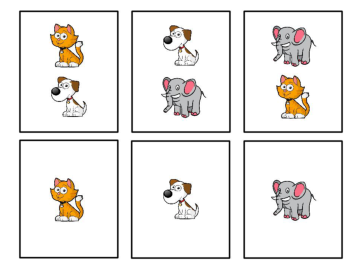
\includegraphics{figs/stimuli-1} 

}

\caption{Cards used in the connective guessing game.}\label{fig:stimuli}
\end{figure}
The materials included six cards with cartoon images of a cat, a dog,
and an elephant (Figure \ref{fig:stimuli}), and the questions were
designed to focus on the type of cards participants saw and the guess
they heard about each one. There were two types of cards: cards with
only one animal pictured and cards with two animals. There were three
types of guesses: simple (e.g. \emph{There is a cat}), conjunctive (e.g.
\emph{There is a cat and a dog}), and disjunctive (e.g. \emph{There is a
cat or a dog}). In each guess, the animal labels used in the guess and
the animal images on the card could have no overlap (e.g.~Image: dog,
Guess: \emph{There is a cat or an elephant}), partial overlap
(e.g.~Image: Cat, Guess: \emph{There is a cat or an elephant}), or total
overlap (e.g.~Image: cat and elephant, Guess: \emph{There is a cat or an
elephant}). Crossing the number of animals on the card, the type of
guess, and the overlap between the guess and the card yields 12
different possible trial types. I chose 8 trial types (Figure
\ref{fig:trials}), to balance the number of one-animal vs.~two-animal
cards, simple vs.~connective guesses, and expected true vs.~false trials
(as shown in Figure \ref{fig:stimuli}).
\begin{figure}[t]

{\centering 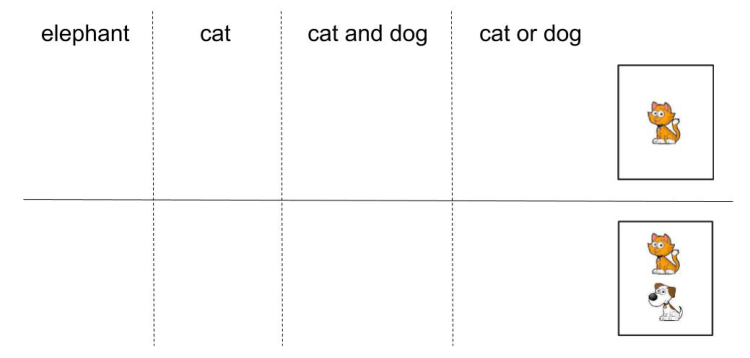
\includegraphics{figs/trials-1} 

}

\caption{Trial types represented by example cards and example guesses.}\label{fig:trials}
\end{figure}
\subsubsection{Participants and
Procedure}\label{participants-and-procedure}
\begin{figure}[t]

{\centering 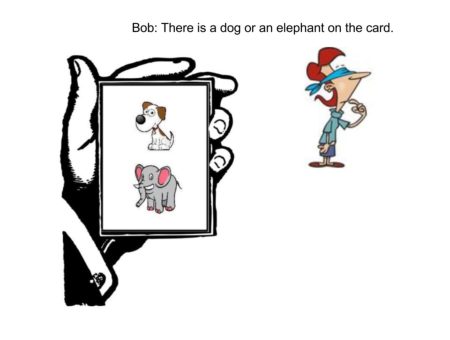
\includegraphics{figs/exampleTrial-1} 

}

\caption{An example trial in the online study.}\label{fig:exampleTrial}
\end{figure}
I used Amazon's Mechanical Turk (MTurk) for recruitment and the online
platform Qualtrics for data collection and survey design. The task took
about 5 minutes on average to complete. 109 English speaking adults
participated. 57 of them were assigned to a 2AFC judgment task and 52 to
a 3AFC judgment task. In the 2AFC task, participants had to judge using
the options \emph{wrong} and \emph{right}. In the 3AFC task they had to
choose between \emph{wrong}, \emph{kinda right}, and \emph{right}. The
two conditions were otherwise identical.

The experiment had three phases: introduction, instruction, and test. In
the introduction, participants saw the six cards and read that they
would play a guessing game. Then a blindfolded cartoon character named
Bob appeared on the screen and they were told that in each round of the
game, they would see a card and Bob was going to guess what animal was
on the card. I emphasized that Bob could not see anything. I asked
participants to judge whether Bob's guess was right. In the instruction
phase, participants saw an example trial where a card with the image of
a dog was shown with the following sentence written above Bob's head:
\emph{Bob: There is a cat on the card}. All participants who correctly
responded with \emph{wrong} proceeded to the test phase.

In the test phase, participants saw one trial per trial type. Within
each trial type, the specific card-guess scenario was chosen at random.
The order of trial types was also randomized. At the end of the study,
participants received \$0.4 as compensation. Figure
\ref{fig:exampleTrial} shows an example test trial.
\begin{longtable}[]{@{}lllll@{}}
\caption{\label{tab:study1info} Summary of Study 1 Methods}\tabularnewline
\toprule
Study & N & Age & Mode & Response Options\tabularnewline
\midrule
\endfirsthead
\toprule
Study & N & Age & Mode & Response Options\tabularnewline
\midrule
\endhead
Study 1 - Part 1 & 57 & Adults & Online (Mturk) & Wrong,
Right\tabularnewline
Study 1 - Part 2 & 52 & Adults & Online (Mturk) & Wrong, Kinda Right,
Right\tabularnewline
\bottomrule
\end{longtable}
\subsection{Results}\label{results}

In this section, I first present the results of the 2AFC and 3AFC tasks
with adults. Then I discuss how these results can be interpreted with
respect to the semantics and pragmatics of disjunction in the context of
the guessing game.

\subsubsection{Two Alternative
Judgments}\label{two-alternative-judgments}
\begin{figure}[t]

{\centering 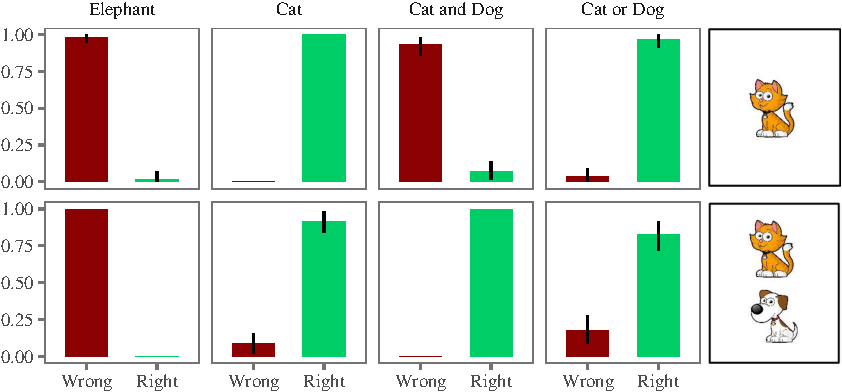
\includegraphics{figs/binaryAdultsPlot-1} 

}

\caption{Adults' two-alternative forced choice judgments.}\label{fig:binaryAdultsPlot}
\end{figure}
Figure \ref{fig:binaryAdultsPlot} shows the results for the adult 2AFC
task. The two left columns show the simple guesses and serve as
controls. The results show that if the animal mentioned in the guess was
not on the card (e.g., elephant), participants judged the guess to be
``wrong''; if the animal was on the card (e.g., cat), participants
judged the guess to be ``right''. The next two columns of Figure
\ref{fig:binaryAdultsPlot} show how the results for the test conditions,
namely conjunction and disjunction, match the expectations for logical
conjunction and (inclusive) disjunction: An \emph{and}-guess (e.g.~cat
and dog) is ``wrong'' if only one of the animals is shown on the card,
and ``right'' if both are on the card. An \emph{or}-guess (e.g.~cat or
dog) is ``right'' whether one or both animals are depicted on the card.

\subsubsection{Three Alternative
Judgments}\label{three-alternative-judgments}
\begin{figure}[t]

{\centering 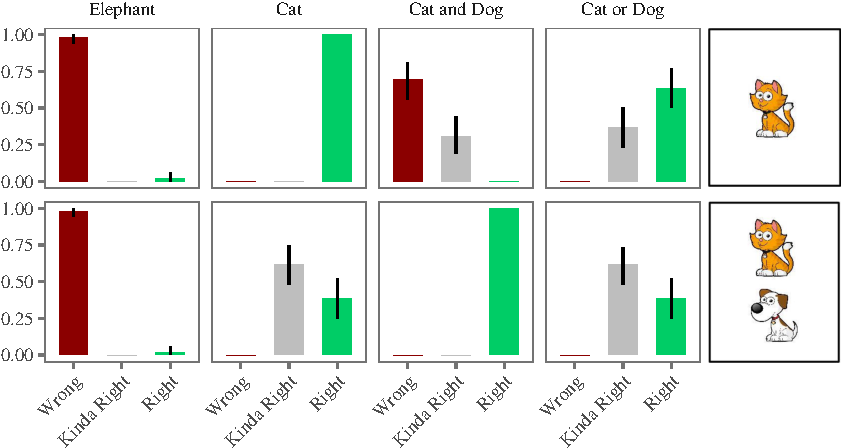
\includegraphics{figs/ternaryAdultsPlot-1} 

}

\caption{Adults' three-alternative forced choice judgments in the connective guessing game.}\label{fig:ternaryAdultsPlot}
\end{figure}
Figure \ref{fig:ternaryAdultsPlot} shows the results for the 3AFC
judgment task. For four trial types, the results are identical to the
2AFC task: if the animal mentioned in the guess was not on the card
(e.g.~elephant), participants judged the guess ``wrong''. If the animal
mentioned (e.g.~cat) was the only animal on the card, participants
judged the guess ``right''. Finally, if there were two animals and the
puppet mentioned them using \emph{and} (e.g.~cat and dog), all
participants considered the guess ``right''.

The four remaining trial types showed different patterns of judgments
than the ones in the 2AFC task. If the animal mentioned (e.g.~cat) was
only one of the animals on the card, participant judgments were divided
between ``right'' and ``kinda right'' (Table \ref{tab:binomStats}, row
1). Also, most adults considered a conjunctive guess (e.g.~cat and dog)
``wrong'', when only one of the animals was on the card (Table
\ref{tab:binomStats}, row 2). However, some considered it \emph{kinda
right}. When both animals were on the card everyone agreed that the
guess was ``right'' -- as in the results for such trials in the 2AFC
task.

With respect to disjunctive guesses like ``cat or dog'', if the card had
only one of the animals, most adults considers the guess ``right'' while
some considered it ``kinda right'' (Table \ref{tab:binomStats}, row 3).
It is possible that the adults who considered such guesses ``kinda
right'' were sensitive to the under-informative nature of a disjunctive
guess when a simple guess would have been more appropriate. If both
animals were on the card, adults were split between ``kinda right'' and
``right'' responses (Table \ref{tab:binomStats}, row 4). The choice of
``kinda right'' over ``right'' in such trials can be interpreted as a
sign that adults were sensitive to the infelicity of a disjunction when
conjunction was more appropriate. However, the scalar reasoning with
\emph{and} and \emph{or} is subtle and in section \ref{implicature} I
discuss the nature of this reasoning in the context of this guessing
game.
\begin{longtable}[]{@{}lllllll@{}}
\caption{\label{tab:binomStats} Exact One-Sided Binomial
Test}\tabularnewline
\toprule
\begin{minipage}[b]{0.24\columnwidth}\raggedright\strut
Trial Type\strut
\end{minipage} & \begin{minipage}[b]{0.07\columnwidth}\raggedright\strut
\(n_{_{right}}/n_{_{total}}\)\strut
\end{minipage} & \begin{minipage}[b]{0.07\columnwidth}\raggedright\strut
\(\hat{p}_{_{right}}\)\strut
\end{minipage} & \begin{minipage}[b]{0.06\columnwidth}\raggedright\strut
\(p_{_{null}}\)\strut
\end{minipage} & \begin{minipage}[b]{0.06\columnwidth}\raggedright\strut
P-value\strut
\end{minipage} & \begin{minipage}[b]{0.08\columnwidth}\raggedright\strut
\(95\%~CI\)\strut
\end{minipage} & \begin{minipage}[b]{0.08\columnwidth}\raggedright\strut
\strut
\end{minipage}\tabularnewline
\midrule
\endfirsthead
\toprule
\begin{minipage}[b]{0.24\columnwidth}\raggedright\strut
Trial Type\strut
\end{minipage} & \begin{minipage}[b]{0.07\columnwidth}\raggedright\strut
\(n_{_{right}}/n_{_{total}}\)\strut
\end{minipage} & \begin{minipage}[b]{0.07\columnwidth}\raggedright\strut
\(\hat{p}_{_{right}}\)\strut
\end{minipage} & \begin{minipage}[b]{0.06\columnwidth}\raggedright\strut
\(p_{_{null}}\)\strut
\end{minipage} & \begin{minipage}[b]{0.06\columnwidth}\raggedright\strut
P-value\strut
\end{minipage} & \begin{minipage}[b]{0.08\columnwidth}\raggedright\strut
\(95\%~CI\)\strut
\end{minipage} & \begin{minipage}[b]{0.08\columnwidth}\raggedright\strut
\strut
\end{minipage}\tabularnewline
\midrule
\endhead
\begin{minipage}[t]{0.24\columnwidth}\raggedright\strut
Two Animals - Simple\strut
\end{minipage} & \begin{minipage}[t]{0.07\columnwidth}\raggedright\strut
32/52\strut
\end{minipage} & \begin{minipage}[t]{0.07\columnwidth}\raggedright\strut
0.62\strut
\end{minipage} & \begin{minipage}[t]{0.06\columnwidth}\raggedright\strut
0.5\strut
\end{minipage} & \begin{minipage}[t]{0.06\columnwidth}\raggedright\strut
0.06\strut
\end{minipage} & \begin{minipage}[t]{0.08\columnwidth}\raggedright\strut
0.49-1\strut
\end{minipage} & \begin{minipage}[t]{0.08\columnwidth}\raggedright\strut
\strut
\end{minipage}\tabularnewline
\begin{minipage}[t]{0.24\columnwidth}\raggedright\strut
One Animal - AND\strut
\end{minipage} & \begin{minipage}[t]{0.07\columnwidth}\raggedright\strut
16/52\strut
\end{minipage} & \begin{minipage}[t]{0.07\columnwidth}\raggedright\strut
0.69\strut
\end{minipage} & \begin{minipage}[t]{0.06\columnwidth}\raggedright\strut
0.5\strut
\end{minipage} & \begin{minipage}[t]{0.06\columnwidth}\raggedright\strut
0.004\strut
\end{minipage} & \begin{minipage}[t]{0.08\columnwidth}\raggedright\strut
0.57-1\strut
\end{minipage} & \begin{minipage}[t]{0.08\columnwidth}\raggedright\strut
\strut
\end{minipage}\tabularnewline
\begin{minipage}[t]{0.24\columnwidth}\raggedright\strut
One Animal - OR\strut
\end{minipage} & \begin{minipage}[t]{0.07\columnwidth}\raggedright\strut
19/52\strut
\end{minipage} & \begin{minipage}[t]{0.07\columnwidth}\raggedright\strut
0.63\strut
\end{minipage} & \begin{minipage}[t]{0.06\columnwidth}\raggedright\strut
0.5\strut
\end{minipage} & \begin{minipage}[t]{0.06\columnwidth}\raggedright\strut
0.04\strut
\end{minipage} & \begin{minipage}[t]{0.08\columnwidth}\raggedright\strut
0.51-1\strut
\end{minipage} & \begin{minipage}[t]{0.08\columnwidth}\raggedright\strut
\strut
\end{minipage}\tabularnewline
\begin{minipage}[t]{0.24\columnwidth}\raggedright\strut
Two Animals - OR\strut
\end{minipage} & \begin{minipage}[t]{0.07\columnwidth}\raggedright\strut
32/52\strut
\end{minipage} & \begin{minipage}[t]{0.07\columnwidth}\raggedright\strut
0.62\strut
\end{minipage} & \begin{minipage}[t]{0.06\columnwidth}\raggedright\strut
0.5\strut
\end{minipage} & \begin{minipage}[t]{0.06\columnwidth}\raggedright\strut
0.06\strut
\end{minipage} & \begin{minipage}[t]{0.08\columnwidth}\raggedright\strut
0.49-1\strut
\end{minipage} & \begin{minipage}[t]{0.08\columnwidth}\raggedright\strut
\strut
\end{minipage}\tabularnewline
\bottomrule
\end{longtable}
\subsection{Discussion}\label{discussion-1}

The example sentences bellow show the common interpretations of
conjunctive and disjunctive assertions (Aloni, 2016).
\begin{itemize}
\tightlist
\item
  Bob is sad \emph{and} angry.
  \begin{itemize}
  \tightlist
  \item
    Both are true. (Truth Conditional Meaning)
  \end{itemize}
\item
  Bob is sad \emph{or} angry.
  \begin{itemize}
  \tightlist
  \item
    At least one of the two is true. (Truth Conditional Meaning)
  \item
    Speaker doesn't know which is true. (Ignorance Inference)
  \item
    At most one of the two is true. (Exclusivity Inference)
  \end{itemize}
\end{itemize}
A conjunctive assertion implies that both propositions are true while a
disjunctive assertion implies that at least one is true. These two
inferences follow from the classical truth-conditional account of
conjunction and disjunction. They constitute the semantics of \emph{and}
and \emph{or}. However, a disjunctive assertion often has two additional
inferences: an ignorance inference and an exclusivity inference. These
additional inferences are often classified as having pragmatic meaning.
This section discusses the semantics and pragmatics of \emph{and} and
\emph{or} in the context of study 1's guessing game.\footnote{See
  Gutzmann (2014) for a comprehensive discussion of the definitions and
  boundaries of semantics and pragmatics. Here my definitions and
  assumptions are close to those of Gazdar (1979).}

\subsubsection{The Semantics of AND and
OR}\label{the-semantics-of-and-and-or}

Let's assume that the semantics of \emph{and} and \emph{or} in simple
declarative sentences like ``there is a cat and/or a dog'' is captured
by the logical operators conjunction and inclusive disjunction
respectively. A conjunction is true when both conjuncts are true and
false otherwise. An inclusive disjunction is true when at least one
disjunct is true and false otherwise. Let's also assume that a false
statement is judged as ``wrong'' and a true statement as ``right''. In
the context of study 1, this purely semantic (i.e.~truth-conditional)
account has two main predictions: 1. Conjunctive guesses like ``cat and
dog'' are wrong when only one of the animals is on the card. 2.
Disjunctive guesses are always right because in all such trials at least
one of the animals is present on the card. Figure
\ref{fig:binaryAdultsPlot} shows that in 2AFC judgments, both
predictions are borne out. In other words, judgments with two
alternatives closely match the predictions of a purely semantic or truth
conditional account of the connectives \emph{and} and \emph{or}. Adults
interpreted ``right'' and ``wrong'' roughly as ``true'' and ``false'' in
the 2AFC task.

However, in the 3AFC task, judgments deviated from a purely semantic
account in four trial types: 1. disjunction trials with one animal 2.
disjunction trials with two animals, 3. conjunction trials with one
animal, and 4. the trials with simple guesses when two animals were
shown on the card. Participants often used the third option \emph{kinda
right} in these trial types. Other trial types obtained identical
results in 2AFC and 3AFC tasks. The comparison of forced choice
judgments with two and three alternatives suggests that two alternatives
better capture the truth-conditional meaning of the connectives, but
underestimate adult pragmatics reasoning.

\subsubsection{The Pragmatics of AND and OR}\label{implicature}
\begin{figure}[t]

{\centering 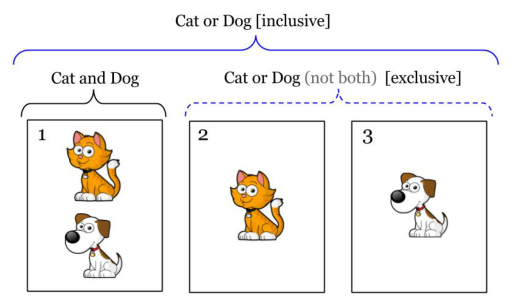
\includegraphics{figs/exclusivity-1} 

}

\caption{Example of cards referred to by a conjunction, inclusive disjunction, and exclusive disjunction.}\label{fig:exclusivity}
\end{figure}
A disjunctive assertion like ``cat or dog'' gives rise to an ignorance
inference and an exclusivity inference. The ignorance inference is the
inference that the speaker does not know which disjunct actually holds.
For example in figure \ref{fig:exclusivity}, the speaker does not know
whether the card has a cat on it or a dog - they are uncertain between
cards 1, 2, and 3. The guessing game in this study controls for the
ignorance inference by keeping the guesser blindfolded. Therefore, all
the disjunctive guesses are evaluated in a context where participants
know that the guesser is ignorant of the animals on the cards - both the
number of them on the card and their identity. The exclusivity inference
is the inference that only one of the disjuncts holds and \textbf{not
both}. In figure \ref{fig:exclusivity}, a disjunction like ``cat or
dog'' only refers to cards 2 and 3 if it is accompanied by an
exclusivity inference.

Since Grice (1989), this exclusive interpretation of ``or'' has been (at
least partly) attributed to pragmatic reasoning about the speaker's
connective choice. The reasoning goes like this: conversational
participants are required to make their utterances as informative as
possible. In the context of making predictions and guessing, a guesser
is required to make their guess as specific (i.e.~informative) as
possible.\footnote{When you ask someone to predict the outcome of a coin
  toss, a guess like ``it will be heads or tails'' does not count as a
  felicitous guess or prediction.} The conjunction word \emph{and} is
more specific and informative than the disjunction word \emph{or} (L.
Horn, 1989). For example in figure \ref{fig:exclusivity}, ``cat and
dog'' picks card 1 while ``cat or dog'' refers to cards 1, 2, and 3. If
a speaker intends to refer to card 1, they should use \emph{and} and say
``cat and dog''. They did not use \emph{and}, so they probably do not
intend to refer to card 1. Following this line of reasoning, I can
\textbf{exclude} the possibility that the speaker intends to refer to
card 1. The term \textbf{exclusivity implicature} captures this
pragmatic reasoning that results in excluding the possibility of both
disjuncts being true.

The goal in this section is to lay out the structure of pragmatic
reasoning in the experimental setup and explain how they can be
manifested in the results of the experimental studies. There are three
main components to the pragmatic reasoning in the guessing game: 1. the
assumptions of the game. 2. sensitivity to (under)informativity, and 3.
the pragmatic reasoning about the speaker's choice of connectives.
Following Katsos \& Bishop (2011), I have considered \textbf{sensitivity
to informativeness} as a precondition for \textbf{derivation of scalar
implicatures}. I begin with the assumptions of the guessing game.
\begin{itemize}
\tightlist
\item
  \textbf{Guessing Game Assumptions}:
  \begin{itemize}
  \tightlist
  \item
    \textbf{Ignorance}: the guesser does not know the number or identity
    of the animals on the card.
  \item
    \textbf{Specificity}: A guesser is required to be as specific as
    possible, ideally referring to a single card.
  \end{itemize}
\end{itemize}
As explained before, ignorance of the guesser is explicitly explained to
the participants. However, specificity is an assumption that was
implicit in the game\footnote{Making this assumption explicit is both
  hard for young children and almost impossible when disjunctive guesses
  are used. Disjunctive guesses are always underinformative and never
  pick out a specific card.}. All the guesses used in the experiment can
pick a single specific card except for disjunctive ones. Conjunctive
guesses like ``cat and dog'' pick specific cards. The simple ones like
``cat'' can be strengthened pragmatically to mean ``only a cat'', and
pick a specific card. However, Disjunctive ones like ``cat or dog'' pick
two cards in their most specific (exclusive) sense. Therefore, they are
always under-informative and violate the specificity assumption.
\begin{itemize}
\tightlist
\item
  \textbf{Sensitivity to Informativeness}: The guesser said ``cat or
  dog'' which is under-informative and picks card 1, 2, and 3.
  \begin{itemize}
  \tightlist
  \item
    \textbf{Violation Assumption}: the guesser is violating the
    specificity requirement.
  \end{itemize}
\end{itemize}
Participants can detect the underinformativity of disjunctive guesses,
notice the violation of specificity, and then decide whether they would
like to tolerate this violation or punish it. It should be pointed out
that it is hard to distinguish between ``tolerating the specificity
violation'' and simply revising the specificity assumption of the game
to avoid a violation. For example, participants may assume that the goal
of the game is saying something true about the cards rather than being
as specific as possible. In either case, the prediction is that adults
who tolerate violation or revise specificity would judge disjunctive
guesses as ``right''. However, if participants assume specificity and
decide to not tolerate its violation, they will judge all disjunctive
guesses to have some degree of infelicity. Since an under-informative
guess is still technically correct, participants may not punish such a
guess with a ``wrong'' response and prefer an intermediate option for
like ``kinda right''. This is what I find in study 1 results. With two
alternatives, not many adults judge infelicity with disjunctive guesses
and I see almost no ``wrong'' responses. With three alternatives,
``kinda right'' responses pop up. Adults responses are split between
``kinda right'' and ``right''.
\begin{figure}[tb]

{\centering 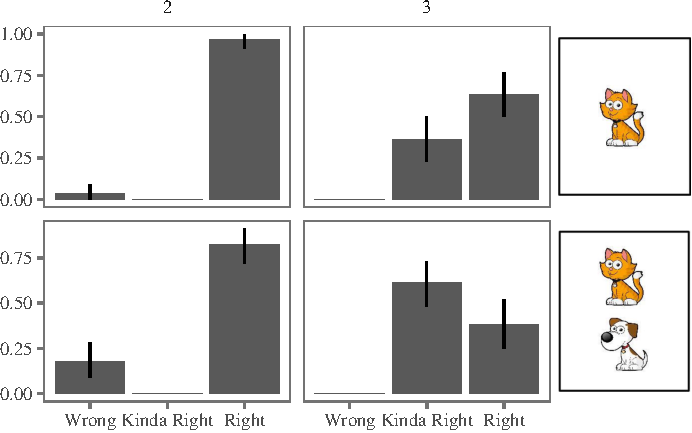
\includegraphics{figs/implicaturePlot-1} 

}

\caption{Adult responses to dicjunction guesses where both discjuncts where true with 2 and 3 options.}\label{fig:implicaturePlot}
\end{figure}
If detecting and reacting to underinformativity is the whole story, then
disjunctive guesses should show similar degrees of infelicity,
regardless of how many animals there are on the card. However, the
results of the 3AFC task suggest otherwise. A logistic mixed-effects
model with the random intercepts and slopes for subjects and fixed
effect of disjunction type found that when comparing disjunctive guesses
in the 3AFC task, participants are more likely to choose \emph{kinda
right} than \emph{right} when both animals were on the card
(\(\beta\)=-1.22, \(z\)=-2.25, \(p\)=0.02). In other words, participants
judged further infelicity with disjunctive guesses that had both
disjuncts as true. Therefore, it is reasonable to assume that when both
disjuncts were true, some participants went through the following
pragmatic reasoning.
\begin{itemize}
\tightlist
\item
  \textbf{Reasoning on Alternatives}: Why did the guesser choose the
  underinformative connective \emph{or} rather than the more informative
  one \emph{and}?
  \begin{itemize}
  \tightlist
  \item
    \textbf{Resolution Assumption}: speaker is trying to be as specific
    as possible by resolving the issue of how many animals are on the
    card.
    \begin{itemize}
    \tightlist
    \item
      \textbf{Exclusivity Implicature}: Given the resolution hypothesis,
      if the speaker had decided that two animals were on the card, they
      should have said ``cat \emph{and} dog''. He did not, so he had
      decided that only one animal is on the card and \textbf{not both}.
    \end{itemize}
  \end{itemize}
\end{itemize}
How does the exclusivity implicature affect participant judgments in the
experimental setting? One possibility is that excluding the correct
response pragmatically is treated like cases of excluding the right
response semantically. For example, guessing ``elephant'' when there is
a cat on the card. The prediction is that disjunctive trials with true
disjuncts should receive ``wrong'' responses. However, this prediction
was not borne out. Such disjunctive trials are almost never judged as
``wrong''.

Alternatively, it is possible that adults differentiate incorrect
pragmatics from incorrect semantics (i.e.~falsehood) and punish
incorrect pragmatics less than incorrect semantics. This conclusion is
supported by the response patterns across trial types (figure
\ref{fig:ternaryAdultsPlot}). Trial types that have received a ``wrong''
response are those that are false. Pragmatically infelicitous trial
types, namely simple guesses like ``cat'' or disjunctive guesses like
``cat or dog'' when both animals are on the card, receive ``kinda
right'' responses. In other words, adults consider false utterances as
``wrong'' guesses but infelicitous utterances do not reach the level of
being ``wrong''; they are still right even though not completely right.
This explains why the rates of infelicity (avoiding the ``right''
alternative) differ between 2AFC and 3AFC trials in disjunctive trials
with true disjuncts (0.18 vs.~0.62).

\section{Study 2: Children's three-alternative judgments and open-ended
corrective
feedback}\label{study-2-childrens-three-alternative-judgments-and-open-ended-corrective-feedback}

The goal of this study was to examine children's interpretations of
\emph{and} and \emph{or} in the guessing game and compare them to those
of the adults. Since the 3AFC judgment task in study 1 proved better at
capturing the nuances in adults' pragmatic reasoning, I decided to first
test children using three alternatives. I also analyzed children's
open-ended comments about the guesses in the experimental context. Both
three-alternative judgments and the analysis of children's open-ended
responses showed that children differentiate \emph{and} and \emph{or}
statements. The judgment task suggested that children do not consider
disjunctive guesses when both disjuncts are truly infelicitous. Yet, the
analysis of their open-ended feedback showed that they did find such
guesses infelicitous. I conclude that the 3AFC judgment task can
underestimate children's pragmatic competence.

\subsection{Methods}\label{methods-1}
\begin{longtable}[]{@{}lllll@{}}
\caption{\label{tab:study2info} Summary of Study 1 and Study 2
Methods}\tabularnewline
\toprule
\begin{minipage}[b]{0.17\columnwidth}\raggedright\strut
Study\strut
\end{minipage} & \begin{minipage}[b]{0.08\columnwidth}\raggedright\strut
N\strut
\end{minipage} & \begin{minipage}[b]{0.16\columnwidth}\raggedright\strut
Age\strut
\end{minipage} & \begin{minipage}[b]{0.15\columnwidth}\raggedright\strut
Mode\strut
\end{minipage} & \begin{minipage}[b]{0.31\columnwidth}\raggedright\strut
Response Option\strut
\end{minipage}\tabularnewline
\midrule
\endfirsthead
\toprule
\begin{minipage}[b]{0.17\columnwidth}\raggedright\strut
Study\strut
\end{minipage} & \begin{minipage}[b]{0.08\columnwidth}\raggedright\strut
N\strut
\end{minipage} & \begin{minipage}[b]{0.16\columnwidth}\raggedright\strut
Age\strut
\end{minipage} & \begin{minipage}[b]{0.15\columnwidth}\raggedright\strut
Mode\strut
\end{minipage} & \begin{minipage}[b]{0.31\columnwidth}\raggedright\strut
Response Option\strut
\end{minipage}\tabularnewline
\midrule
\endhead
\begin{minipage}[t]{0.17\columnwidth}\raggedright\strut
Study 1 - Part 1\strut
\end{minipage} & \begin{minipage}[t]{0.08\columnwidth}\raggedright\strut
57\strut
\end{minipage} & \begin{minipage}[t]{0.16\columnwidth}\raggedright\strut
Adults\strut
\end{minipage} & \begin{minipage}[t]{0.15\columnwidth}\raggedright\strut
Online (Mturk)\strut
\end{minipage} & \begin{minipage}[t]{0.31\columnwidth}\raggedright\strut
Wrong, Right\strut
\end{minipage}\tabularnewline
\begin{minipage}[t]{0.17\columnwidth}\raggedright\strut
Study 1 - Part 2\strut
\end{minipage} & \begin{minipage}[t]{0.08\columnwidth}\raggedright\strut
52\strut
\end{minipage} & \begin{minipage}[t]{0.16\columnwidth}\raggedright\strut
Adults\strut
\end{minipage} & \begin{minipage}[t]{0.15\columnwidth}\raggedright\strut
Online (Mturk)\strut
\end{minipage} & \begin{minipage}[t]{0.31\columnwidth}\raggedright\strut
Wrong, Kinda Right, Right\strut
\end{minipage}\tabularnewline
\begin{minipage}[t]{0.17\columnwidth}\raggedright\strut
Study 2\strut
\end{minipage} & \begin{minipage}[t]{0.08\columnwidth}\raggedright\strut
42\strut
\end{minipage} & \begin{minipage}[t]{0.16\columnwidth}\raggedright\strut
3;1-5;2 (M = 4;3)\strut
\end{minipage} & \begin{minipage}[t]{0.15\columnwidth}\raggedright\strut
Study Room\strut
\end{minipage} & \begin{minipage}[t]{0.31\columnwidth}\raggedright\strut
Circle (wrong), Little Star (little right), Big Star (right)\strut
\end{minipage}\tabularnewline
\bottomrule
\end{longtable}
\subsubsection{Materials and Design}\label{materials-and-design-1}

I used the same set of cards and linguistic stimuli as the ones in study
1. There were 8 trial types and 2 trials per trial type for a total of
16 trials. I made two changes to make the experiment more suitable for
children. First, instead of the fictional character Bob, a puppet named
Jazzy played the guessing game with the children. Jazzy had a sleeping
mask on his eyes during the game (Figure \ref{fig:jazzy}). Second, a
pilot study showed that a scale with three alternatives is better
understood and used by children if it is presented in the form of
rewards to the puppet rather than verbal responses such as ``wrong'',
``a little bit right'', and ``right'', or even hand gestures such as
thumbs up, middle, and down. Therefore, I placed a set of red circles,
small blue stars, and big blue stars in front of the children. These
tokens were used to reward the puppet after each guess. During the
introduction, the experimenter explained that if the puppet is right,
the child should give him a big star, if he is a little bit right, a
little star, and if he is not right, the puppet gets a red circle.
\begin{figure}[tb]

{\centering 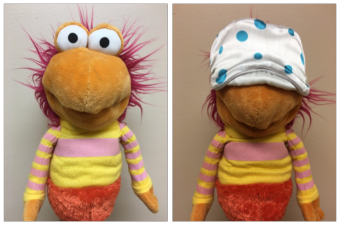
\includegraphics{figs/jazzy-1} 

}

\caption{Jazzy with and without the sleeping mask.}\label{fig:jazzy}
\end{figure}
\subsubsection{Participants and
Procedure}\label{participants-and-procedure-1}

I recruited 42 English speaking children from the Bing Nursery School at
Stanford University. Children were between 3;1 and 5;2 years old (Mean =
4;3). The experiment was carried out in a quiet room and all sessions
were videotaped. There was a small table and two chairs in the room.
Children sat on one side of the table and the experimenter and the
puppet on the other side facing the child. The groups of circles, small
stars, and big stars were placed in front of the child from left to
right. A deck of six cards was in front of the experimenter. As in study
1 with adults, the children sat through three phases: introduction,
instruction, and test.

The goal of the introduction was to show the cards to children and make
sure they recognized the animals and knew their names. The experimenter
showed the cards to the children and asked them to label each animal.
All children recognized the animals and could label them correctly. In
the instruction phase, children went through three example trials. The
experimenter explained that he was going to play with the puppet first
so that the child could learn the game. He removed the six introduction
cards and placed a deck of three cards face-down on the table. From top
to bottom (first to last), the cards had the following images: cat,
elephant, cat and dog. He put the sleeping mask on the puppet's eyes and
explained that he is going to guess what animal is on the cards. He then
picked the first card and asked the puppet: ``\emph{What do you think is
on this card?}'' The puppet replied with ``\emph{There is a dog}''. The
experimenter showed the cat-card to the child and explained that when
the puppet is \emph{not right} he gets a circle. He then asked the child
to give the puppet a circle. Rewards were collected by the experimenter
and placed under the table to not distract the child. The second trial
followed the same pattern except that the puppet guessed \emph{right}
and the experimenter invited the child to give the puppet a big star. In
the final trial, the puppet guessed that there is a cat on the card when
the card had a cat and a dog on it. The experimenter said that the
puppet was \emph{a little right} and asked the child to give him a
little star.
\begin{longtable}[]{@{}lll@{}}
\caption{\label{tab:instruction} Instruction Trials.}\tabularnewline
\toprule
Card & Guess & Reward\tabularnewline
\midrule
\endfirsthead
\toprule
Card & Guess & Reward\tabularnewline
\midrule
\endhead
CAT & there is a cat! & Circle\tabularnewline
ELEPHANT & there is an elephant! & Big Star\tabularnewline
CAT-DOG & there is a dog! & Little Star\tabularnewline
\bottomrule
\end{longtable}
In the test phase, the experimenter removed the three instruction cards
and placed a deck of 16 randomized cards on the table. The experimenter
explained that it was the child's turn to play with the puppet. The test
phase followed the pattern described in the instruction phase. You can
find the randomization code as well as the details of the methods on the
online repository for this study.

\subsubsection{Offline Annotations}\label{feedbackCoding}

During analysis of the videos, children's linguistic feedback to the
puppet after each guess was categorized into four types: 1. None, 2.
Judgments, 3. Descriptions, and 4. Corrections. The first category
referred to cases where children did not say anything and only rewarded
the puppet. Judgments referred to linguistic feedback such as \emph{you
are right!}, \emph{yes}, \emph{nope}, or \emph{you winned}. Such
feedback only expressed judgments and complemented the rewards.
Descriptions were cases that the child simply mentioned what was on the
card: \emph{cat!}, \emph{dog and elephant!}, \emph{There is a cat and a
dog!} etc. Finally, corrections referred to feedback that provided
additional linguistic elements that acted like corrections to what the
puppet had said. Examples include: \emph{Just a cat!}, \emph{Both!},
\emph{The two are!}, \emph{Only cat}, \emph{cat AND dog} (with emphasis
placed on \emph{and}). In trials where the child provided both judgments
as well as descriptions or corrections, I placed the feedback into the
more informative categories, namely description or correction.

\subsection{Results}\label{results-1}
\begin{figure}[t]

{\centering 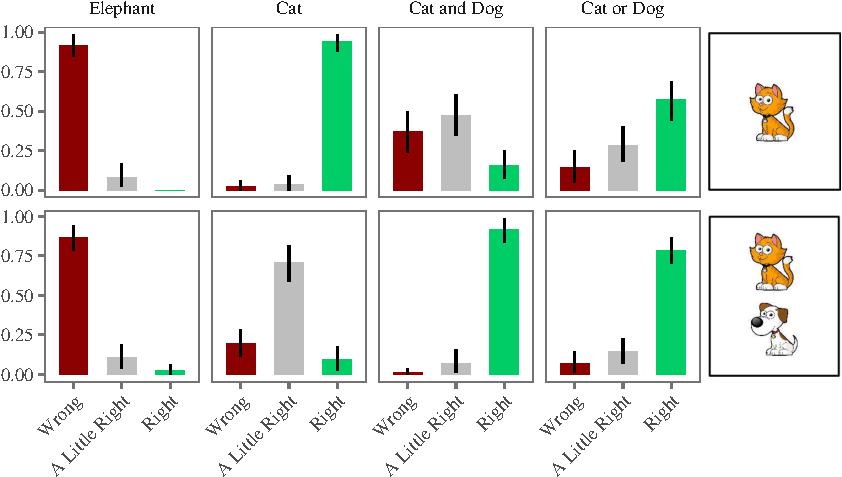
\includegraphics{figs/childrenTernaryPlot-1} 

}

\caption{Children's ternary judgments in the connective guessing game.}\label{fig:childrenTernaryPlot}
\end{figure}
Figure \ref{fig:childrenTernaryPlot} shows the results for children's
3AFC judgments. Starting from the left column, we see that if the
mentioned animal was not on the card (e.g.~elephant), children judged
the guess to be ``wrong''. If the animal mentioned (e.g.~cat) was the
only animal on the card, children judged the guess to be ``right''. Here
I will ignore the results for trial types in which the animal mentioned
was one of the animals on the card. The reason is that such trials were
used in the instruction phase to introduce the ``little bit right''
guesses, and the results are potentially biased by the instructions.

In conjunctive guesses (e.g. \emph{cat and dog}), when only one of the
animals mentioned was on the card, children judged the guess as
``wrong'' or ``a little bit right''. However, if both animals were on
the card, they judged the conjunctive guess as ``right''. In disjunctive
guesses (e.g. \emph{cat or dog}), when only one of the animals mentioned
was on the card, children considered the guess ``right'' or ``kinda
right''. If both animals were on the card, the disjunctive guess was
considered ``right''.

Comparison of the conjunction and disjunction trials (last two columns
of figure \ref{fig:childrenTernaryPlot}) shows that overall, children
distinguished between \emph{and} and \emph{or} guesses in cases when one
animal was on the card but not when both were. Given that the one-animal
conjunction trials and the one-animal disjunction trials differ in truth
conditions, the difference in response patterns suggests that children
at this age have a different semantic knowledge for \emph{and} and
\emph{or}. The two-animal conjunction and two-animal disjunction trials
did not differ in truth values, and the responses also show no
difference.

In the one-animal and two-animal trials (figure
\ref{fig:childrenTernaryPlot} rows), children gave different responses
when the guess contained the conjunction word \emph{and} but not when
\emph{or} is used. Since the truth values of one-animal and two-animal
trials differ for conjunctive guesses but not disjunctive ones, the
results suggest that children were sensitive to the difference in
meaning between \emph{and} and \emph{or}. The similarity of the
disjunctive guesses in one-animal and two-animal trials could also be
interpreted as a lack of pragmatic reasoning in children.
\ref{fig:childAdultComp} compares the results for children and adults'
3AFC judgments in the conjunction and disjunction trials. The major
difference between adults and children's responses here is visible in
the disjunctive trials where both animals were on the card; in other
words, trials where both disjuncts are true. In the next section, I use
statistical modeling to compare adults' and children's three-alternative
responses more systematically.
\begin{figure}[t]

{\centering 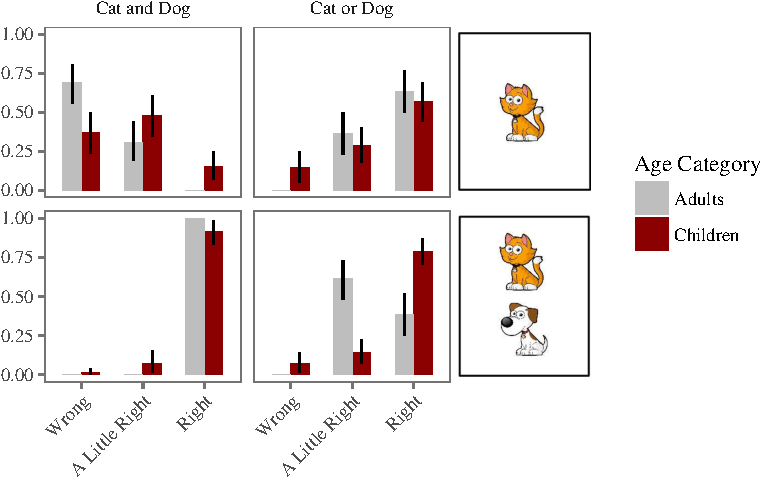
\includegraphics{figs/childAdultComp-1} 

}

\caption{Comparison of Adults' and Children's ternary judgments.}\label{fig:childAdultComp}
\end{figure}
\subsubsection{Analysis and Statistical
Modeling}\label{analysis-and-statistical-modeling}
\begin{figure}[t]

{\centering 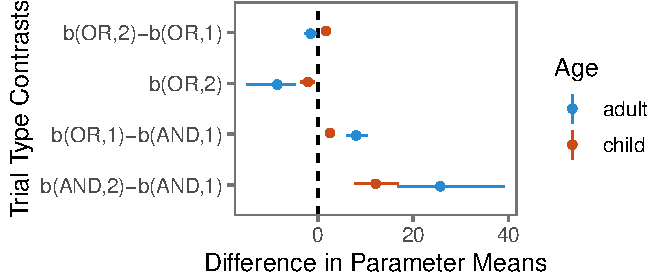
\includegraphics{figs/stanModelPlot-1} 

}

\caption{Coefficients capturing the relevant comparisons across conditions in ternary judgments in Study 1 and 2. Error bars represent 99\% regions of highest posterior density.}\label{fig:stanModelPlot}
\end{figure}
I used the R package \emph{\{rstan\}} for Bayesian statistical modeling
to fit separate ordinal mixed-effects logistic models for the children's
and adults' judgments. The response variable had three ordered levels:
\emph{wrong}, \emph{kinda right}, and \emph{right}. The trial types
\emph{One-Animal-OR}, \emph{Two-Animals-OR}, \emph{One-Animal-AND}
constituted the (dummy-coded) fixed effects of the model with
\emph{Two-Animals-AND} set as the intercept. The model also included
by-subject random intercepts. The priors over trial types and the random
intercepts were set to \(\mathcal{N}(0,10)\). I also included parameters
\(C_1\) and \(C_2\), the two cutpoints delimiting the logistic for 1)
\emph{wrong} and \emph{kinda right} and 2) \emph{kinda right} and
\emph{right} responses, drawn with the prior
\(\mathcal{N}(0,1)\).\footnote{I used a tight prior in this case to
  decrease posterior correlations between cutpoints and intercept.} All
four chains converged after 3000 samples (with a burn-in period of 1500
samples)

I made inferences based on the highest-posterior density (HPD) intervals
for the coefficients estimated from each model. Because predictors are
dummy-coded, it's possible to examine contrasts of interest by computing
the difference between coefficients for pairs of conditions I wish to
contrast. Figure \ref{fig:stanModelPlot} shows the contrasts of
interest: \emph{b(OR, 2)-b(OR,1)} represents the difference between the
estimated coefficients for the disjunction trials with two animal on the
card and those with only one; \emph{b(OR, 2)} represents the difference
between the estimated coefficients for the conjunction trials with two
animals and the disjunction trials with two animals; and so on.

Overall, adults' and children's estimated coefficients are similar in
sign to one another, though adults' are more extreme. In the conjunction
trials (\emph{b(AND, 2)-b(AND,1)}), children and adults showed a strong
preference for the cards with two animals rather than one. At the same
time, given two animals on the card, children and adults showed a
preference for \emph{and} rather than \emph{or} (\emph{b(OR, 2)}).
However, with only one animal on the card, children and adults preferred
a disjunctive guess (\emph{b(OR, 1)-b(AND,1)}). These results are
compatible with the truth conditions of conjunction and disjunction.

The main difference between adults and children shows up in the contrast
between the disjunctive trial types: two animals vs.~only one
(\emph{b(OR, 2)-b(OR,1)}). On average, children rated disjunction trials
with two animals higher than those with only one. Adults on the other
hand showed the opposite pattern: they rated disjunction trials with two
animals lower. This pattern is compatible with current accounts of
pragmatic development that suggest an absence of implicatures in
children's interpretations. The idea is that while adults strengthen the
disjunctive guess ``cat or dog'' to ``cat or dog but not both'',
children simply interpret it as ``cat or dog or both''. Adults are
therefore going to rate trials where both disjuncts are true as lower.

The slight preference children show for cards with two animals when the
guess is disjunctive is also compatible with the account proposed by
Singh et al. (2016) and L. Tieu et al. (2016). However, the effect is
much smaller here than they reported in their studies. The comparison
with conjunction trials makes it clear that overall, children are not
interpreting \emph{or} as having a conjunctive meaning. The effect in
this study can be more accurately described as a preference for both
disjuncts being true rather than a conjunctive interpretation of
disjunction. I will further discuss the nature of this preference in the
General Discussion.

\subsubsection{Children's open-ended
feedback}\label{childrens-open-ended-feedback}
\begin{longtable}[]{@{}lll@{}}
\caption{\label{tab:feedbackCat} Definitions and Examples for the Feedback
Categories.}\tabularnewline
\toprule
\begin{minipage}[b]{0.16\columnwidth}\raggedright\strut
Category\strut
\end{minipage} & \begin{minipage}[b]{0.44\columnwidth}\raggedright\strut
Definition\strut
\end{minipage} & \begin{minipage}[b]{0.24\columnwidth}\raggedright\strut
Examples\strut
\end{minipage}\tabularnewline
\midrule
\endfirsthead
\toprule
\begin{minipage}[b]{0.16\columnwidth}\raggedright\strut
Category\strut
\end{minipage} & \begin{minipage}[b]{0.44\columnwidth}\raggedright\strut
Definition\strut
\end{minipage} & \begin{minipage}[b]{0.24\columnwidth}\raggedright\strut
Examples\strut
\end{minipage}\tabularnewline
\midrule
\endhead
\begin{minipage}[t]{0.16\columnwidth}\raggedright\strut
None\strut
\end{minipage} & \begin{minipage}[t]{0.44\columnwidth}\raggedright\strut
no feedback provided to the puppet, only reward\strut
\end{minipage} & \begin{minipage}[t]{0.24\columnwidth}\raggedright\strut
\strut
\end{minipage}\tabularnewline
\begin{minipage}[t]{0.16\columnwidth}\raggedright\strut
Judgment\strut
\end{minipage} & \begin{minipage}[t]{0.44\columnwidth}\raggedright\strut
the child said yes/no, you are right, etc.\strut
\end{minipage} & \begin{minipage}[t]{0.24\columnwidth}\raggedright\strut
``No!'' , ``You are right Jazzy!''\strut
\end{minipage}\tabularnewline
\begin{minipage}[t]{0.16\columnwidth}\raggedright\strut
Description\strut
\end{minipage} & \begin{minipage}[t]{0.44\columnwidth}\raggedright\strut
mentioned the animal(s) on the card\strut
\end{minipage} & \begin{minipage}[t]{0.24\columnwidth}\raggedright\strut
``elephant'', ``cat and dog''\strut
\end{minipage}\tabularnewline
\begin{minipage}[t]{0.16\columnwidth}\raggedright\strut
Correction\strut
\end{minipage} & \begin{minipage}[t]{0.44\columnwidth}\raggedright\strut
used focus particles like ``only''/``just'', emphasized ``and'' or used
``both''\strut
\end{minipage} & \begin{minipage}[t]{0.24\columnwidth}\raggedright\strut
``only cat'', ``just elephant'', ``Both!'', ``cat AND dog!''\strut
\end{minipage}\tabularnewline
\bottomrule
\end{longtable}
As explained in section \ref{feedbackCoding}, I also categorized and
annotated children's spontaneous and free form verbal reactions to the
puppet's guesses. Table \ref{tab:feedbackCat} summarizes the definitions
and examples for each category and figure \ref{fig:feedbackData} shows
the results.
\begin{figure}[h]

{\centering 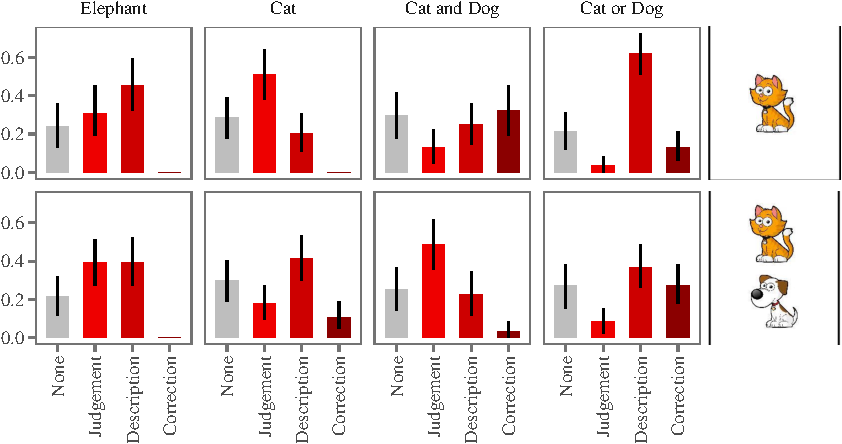
\includegraphics{figs/feedbackData-1} 

}

\caption{Children's open-ended Feedback. Error bars represent 95\% confidence intervals.}\label{fig:feedbackData}
\end{figure}
I should first point out that each trial type shows similar number of
``None'' cases, for feedback. Some children remained more or less silent
throughout the experiment and only provided rewards to the puppet. In
the next study I focus on children's open-ended feedback. In the
discussion and analysis here I will not comment further on the ``None''
category but focus on the other three categories.

In the leftmost column, when the animal guessed (i.e.~elephant) was not
on the card, children either provided judgments like ``No!'' or
described what was on the card like ``cat'' or ``cat and dog''. However,
when the animal guessed was the only animal on the card (i.e.~cat), most
children provided a positive judgment like ``Yes''. When the animal
guessed was only one of the animals on the card, children described what
was on the card, say, ``cat and dog''. Corrections were rare for all
these four control trial types.

In the critical trial types with conjunction and disjunction, children
showed a high rate of corrections and description when the guess used
``and'' but there was only one animal on the card. In their corrections,
children used the focus particles ``just'' and ``only'' like ``just a
cat'' or ``only a cat''. However, in trial types where conjunction was
used and both animals were on the card, children predominantly provided
positive judgments like ``Yes!'' and ``You are right''. Considering
disjunctive guesses like ``cat or dog'', when only one of the animals
was on the card, most children simply described what was on the card,
for example ``cat''. However, when both animals were on the card,
children corrected the puppet by saying ``both'' or emphasizing ``and''
as in ``cat AND dog''.

I performed chi-squared goodness-of-fit tests to compare the feedback
distributions in the critical conditions with ``and'' and ``or''. Here I
focus on those trials (the four bar charts on the right of figure
\ref{fig:feedbackData}). Children's linguistic feedback showed three
patterns. First, the one-animal conjunctive and two-animal disjunctive
(top left and bottom right) trials contained a higher proportion of
Corrections than the other trial types. These were trials where the
guesses were either false or infelicitous. In the conjunction trials, a
comparison of the feedback distribution in one-animal and two-animal
conditions was statistically significant (\(\chi\)(3, 83) = 201.65, p
\textless{} .0001), that children gave different feedback for false
guesses. A similar numerical trend was present in the disjunction
trials, but was not significant (\(\chi\)(9, 4) = 12, p = 0.21).

Second, the one-animal disjunctive trials (top right) showed the highest
proportion of \emph{Descriptions}. These are trials in which the guess
is correct but not specific enough: it leaves two possibilities open.
These trials were significantly different from the one-animal trials for
conjunction (\(\chi\)(3, 83) = 62.16, p \textless{} .0001). Finally, the
two-animal conjunctive trials (bottom left) showed the highest
proportion of \emph{Judgments} such as \emph{You are right!}. This was
not surprising given that in these trials represented the most optimal
guessing scenario. These trials had a significantly different feedback
distribution from the matching disjunction trials (\(\chi\)(3, 84) =
184.98, p \textless{} .0001).

\subsection{Discussion}\label{discussion-2}

In study 2, I used a 3AFC judgment task to test children's comprehension
of logical connectives \emph{and} and \emph{or}. I compared these
results to those found in the 3AFC judgment task of study 1 with adults.
The general comparison showed that adults and children had similar
patterns of judgments, except when both disjuncts were true. In such
cases, adults judged the disjunctive guess as not completely right while
most children found it completely right. There was even a slight
preference among children to rewarded the puppet more in such cases,
compared to cases of disjunction when only one disjunct was true.

To consider another measure of children's comprehension, I also looked
at children's spontaneous open-ended feedback in response to the
guesses. My analysis suggested that children recognized false and
infelicitous utterances with the connectives and provided appropriate
corrective feedback. As expected from an adult-like understanding of
connectives, children corrected the puppet most often when there was
only one animal on the card and the guess was conjunctive, or when there
were two animals on the card and the guess was disjunctive. Perhaps the
most important finding was that children increased their corrective
feedback in disjunctive guesses where both disjuncts were true, compared
to those with only one true disjunct. These findings difer from the the
results of the 3AFC judgment task which suggested that children did not
find any infelicity with disjunctive guesses when both disjuncts were
true.

The analysis of children's open-ended feedback raises two important
issues. First, as I mentioned before, it runs counter to what the 3AFC
judgment task suggests with respect to exclusivity implicatures
(i.e.~trials with disjunction when both disjuncts are true). The
forced-choice judgment task suggests that children find such cases
unproblematic while analysis of their spontaneous feedback shows that
they provided more corrections to the puppet. Second, a common
explanation for why children fail at deriving implicatures is that they
cannot access the stronger alternative to the disjunction \emph{or},
namely \emph{and} (Barner et al., 2011). However, in the context of the
guessing game, some children explicitly mentioned the word \emph{and} as
what the puppet should have said instead of \emph{or}. Interestingly,
these children continued to reward the puppet and considered the guess
``right''. This raises the possibility that children's forced-choice
truth value judgments, whether with two or three alternatives, do not
fully reflect their pragmatic knowledge. In study 3, I decided to make
children's open-ended feedback the main dependent variable of study and
directly compare this to a 2AFC truth judgment in the same task. This
design allowed me to directly compare children's open-ended and forced
choice responses.

\section{Study 3: Children's 2AFC judgments and open-ended
feedback}\label{study-3-childrens-2afc-judgments-and-open-ended-feedback}

This study used the same paradigm as study 2 but focused on children's
open-ended feedback and aimed at replicating the findings in study 2.
The main hypothesis was that four-year-olds provide corrective feedback
to the puppet if both disjuncts are true, but they do not consider this
infelicity to be grave enough to render the guess ``wrong''. The main
hypothesis along with relevant analyses and predictions were
preregistered in an ``As Predicted'' format\footnote{The As Predicted
  pdf document is accessible at \url{https://aspredicted.org/x9ez2.pdf}.}.
The study used a 2AFC judgment task to compare with the open-ended
feedback results. The prediction was that children will provide
corrective feedback to the puppet when both disjuncts were true, yet
consider the guess ``right'' and not reflect this infelicity in truth
value judgments. This is what the study found.

\subsection{Methods}\label{methods-2}
\begin{longtable}[]{@{}lllll@{}}
\caption{\label{tab:study3info} Summary of Study 1, 2, and 3
Methods}\tabularnewline
\toprule
\begin{minipage}[b]{0.19\columnwidth}\raggedright\strut
Study\strut
\end{minipage} & \begin{minipage}[b]{0.02\columnwidth}\raggedright\strut
N\strut
\end{minipage} & \begin{minipage}[b]{0.20\columnwidth}\raggedright\strut
Age\strut
\end{minipage} & \begin{minipage}[b]{0.11\columnwidth}\raggedright\strut
Mode\strut
\end{minipage} & \begin{minipage}[b]{0.32\columnwidth}\raggedright\strut
Response Options\strut
\end{minipage}\tabularnewline
\midrule
\endfirsthead
\toprule
\begin{minipage}[b]{0.19\columnwidth}\raggedright\strut
Study\strut
\end{minipage} & \begin{minipage}[b]{0.02\columnwidth}\raggedright\strut
N\strut
\end{minipage} & \begin{minipage}[b]{0.20\columnwidth}\raggedright\strut
Age\strut
\end{minipage} & \begin{minipage}[b]{0.11\columnwidth}\raggedright\strut
Mode\strut
\end{minipage} & \begin{minipage}[b]{0.32\columnwidth}\raggedright\strut
Response Options\strut
\end{minipage}\tabularnewline
\midrule
\endhead
\begin{minipage}[t]{0.19\columnwidth}\raggedright\strut
Study 1 - Part 1\strut
\end{minipage} & \begin{minipage}[t]{0.02\columnwidth}\raggedright\strut
57\strut
\end{minipage} & \begin{minipage}[t]{0.20\columnwidth}\raggedright\strut
Adults\strut
\end{minipage} & \begin{minipage}[t]{0.11\columnwidth}\raggedright\strut
Online (Mturk)\strut
\end{minipage} & \begin{minipage}[t]{0.32\columnwidth}\raggedright\strut
Wrong, Right\strut
\end{minipage}\tabularnewline
\begin{minipage}[t]{0.19\columnwidth}\raggedright\strut
Study 1 - Part 2\strut
\end{minipage} & \begin{minipage}[t]{0.02\columnwidth}\raggedright\strut
52\strut
\end{minipage} & \begin{minipage}[t]{0.20\columnwidth}\raggedright\strut
Adults\strut
\end{minipage} & \begin{minipage}[t]{0.11\columnwidth}\raggedright\strut
Online (Mturk)\strut
\end{minipage} & \begin{minipage}[t]{0.32\columnwidth}\raggedright\strut
Wrong, Kinda Right, Right\strut
\end{minipage}\tabularnewline
\begin{minipage}[t]{0.19\columnwidth}\raggedright\strut
Study 2\strut
\end{minipage} & \begin{minipage}[t]{0.02\columnwidth}\raggedright\strut
42\strut
\end{minipage} & \begin{minipage}[t]{0.20\columnwidth}\raggedright\strut
3;1-5;2 (M = 4;3)\strut
\end{minipage} & \begin{minipage}[t]{0.11\columnwidth}\raggedright\strut
Study Room\strut
\end{minipage} & \begin{minipage}[t]{0.32\columnwidth}\raggedright\strut
Circle (Wrong), Little Star (Little Right), Big Star (Right)\strut
\end{minipage}\tabularnewline
\begin{minipage}[t]{0.19\columnwidth}\raggedright\strut
Study 3\strut
\end{minipage} & \begin{minipage}[t]{0.02\columnwidth}\raggedright\strut
50\strut
\end{minipage} & \begin{minipage}[t]{0.20\columnwidth}\raggedright\strut
3;6-5;9 (M = 4;7)\strut
\end{minipage} & \begin{minipage}[t]{0.11\columnwidth}\raggedright\strut
Study Room\strut
\end{minipage} & \begin{minipage}[t]{0.32\columnwidth}\raggedright\strut
Yes (Right)/No (Wrong) - Open-ended Feedback\strut
\end{minipage}\tabularnewline
\bottomrule
\end{longtable}
\subsubsection{Materials and Design}\label{materials-and-design-2}

Study 3 was similar to Study 2 but differed in how children provided
their judgments. Based on the findings in Study 2, I focused on verbal
judgments and feedback, instead of rewards. I used two different ways of
measuring children's judgments. First, I encouraged children to provide
verbal feedback to the puppet. They were asked to say ``yes'' when the
puppet was right, and ``no'' when he was not. They were also encouraged
to help the puppet say it better when he was not right. After children
were done with this initial open-ended feedback, for each trial we asked
them a forced choice yes/no judgment question: ``Was Jazzy (the puppet)
right?''. This question elicited a ``yes'' or ``no'' response for each
trial independent of their earlier open-ended response. These two
measures allowed me to compare open-ended and forced choice judgments.

\subsubsection{Participants and
Procedure}\label{participants-and-procedure-2}

I recruited 50 English speaking children from the Bing Nursery School at
Stanford University. Children were between 3;6 and 5;9 years old (Mean =
4;7). The setup and procedure were similar to Study 2, except there were
no rewards on the table. As before, participants sat through three
phases: introduction, instruction, and test. The introduction phase made
sure children knew the names of the animals on the cards. In the
instruction phase, they received four training trials, as shown in table
\ref{tab:instructionStudy3}.

As in Study 2, the experimenter put the sleeping mask over the puppet's
eyes and explained that Jazzy (the puppet) was going to guess what
animal was on the cards. He then picked the first card and asked the
puppet: ``\emph{What do you think is on this card?}'' The puppet replied
with ``\emph{There is a dog}''. The experimenter showed the cat-card to
the child and said: when Jazzy is \emph{not right}, tell him ``No''. He
then asked the child to say ``no'' to the puppet. The second trial
followed the same pattern except that the puppet guessed \emph{right}
and the experimenter invited the child to say ``yes'' to the puppet.
There were two more instruction trials trials before the test phase
began. This contained 16 randomized trials, half of which contained
guesses with the words ``and'' and ``or''.{[}\^{}4{]}

{[}\^{}4{]}You can find the randomization code as well as the details of
the methods on the online repository for this dissertation.
\begin{longtable}[]{@{}lll@{}}
\caption{\label{tab:instructionStudy3} Instruction Trials for Study
3.}\tabularnewline
\toprule
Card & Guess & Response\tabularnewline
\midrule
\endfirsthead
\toprule
Card & Guess & Response\tabularnewline
\midrule
\endhead
CAT & there is a dog! & No!\tabularnewline
ELEPHANT & there is an elephant! & Yes!\tabularnewline
DOG-ELEPHANT & there is a cat! & No!\tabularnewline
DOG & there is a dog! & Yes!\tabularnewline
\bottomrule
\end{longtable}
\subsection{Results}\label{results-2}

Here I first look at the results of the 2AFC judgement task for each
trial type and compare them to those of the adults' in Study 1. Then I
will analyze children's open-ended responses and compare them to the
forced choice responses obtained in the same trials.

For the 2AFC judgments I excluded 26 trials (out of total 800) where
children either did not provide a Yes/No response or provided both (i.e.
``Yes and No''). The exclusions were almost equally distributed among
different types of guesses and cards. In my analysis of children's
open-ended feedback, I excluded 8 trials (out of total 800) where
children either did not provide any feedback or their feedback could not
be categorized into the existing categories.

\subsubsection{Two-Alternative Forced Choice
Judgments}\label{two-alternative-forced-choice-judgments}
\begin{figure}[t]

{\centering 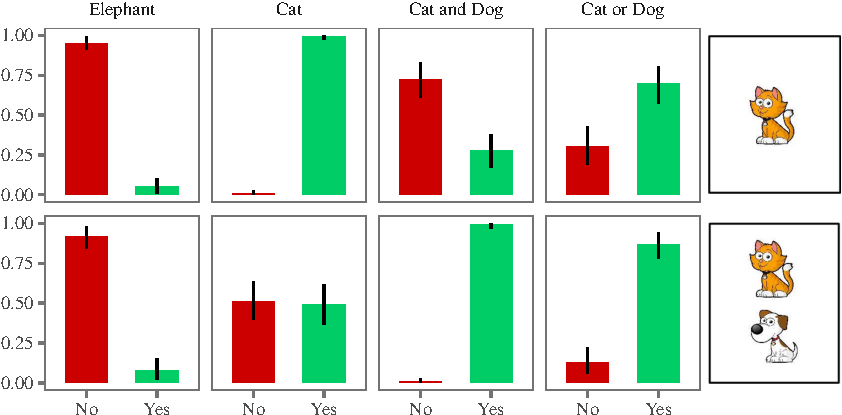
\includegraphics{figs/Study3tvjtPlot-1} 

}

\caption{Children's binary truth value judgments.}\label{fig:Study3tvjtPlot}
\end{figure}
Figure \ref{fig:Study3tvjtPlot} shows children's 2AFC judgments. In the
leftmost column, when the animal guessed (e.g.~elephant) was not on the
card, children considered the guess ``wrong''. When the animal guessed
(e.g.~cat) was the only animal on the card, children considered the
guess ``right''. However, if the animal guessed (e.g.~cat) was only one
of the animals on the card, children were equally split between
``wrong'' and ``right'' judgments. On the other hand, almost all adults
considered such guesses ``right'' in their 2AFC judgments (Figure
\ref{fig:binaryAdultsPlot}). In such trial types, children seem to
interpret the guess ``there is a cat'' as ``there is \textbf{only} a
cat'', while adults do not. This difference between children and adults
is unexpected for a theory of meaning acquisition that assumes children
are overall more logical/literal interpreters than adults (Noveck,
2001).

In the trials with \emph{and} and \emph{or}, we see that children's
judgments were similar to those of adults'. Figure
\ref{fig:BinaryPlotComp} compares adults' and children's 2AFC judgments.
In trials with conjunction, when only one of the animals was on the
card, most children considered the guess ``wrong''. This is similar to
adults' judgments, and different in extent: adults were more consistent
and unanimously rejected such guesses. A mixed effects logistic
regression with the fixed effect of age category (adult vs.~child) and
random effect of subject found no significant difference between adults'
and children's responses in such trials (see Table
\ref{tab:statsStudy3}, Conjunction - One Animal).
\begin{longtable}[]{@{}lcccc@{}}
\caption{\label{tab:statsStudy3} Mixed effects logistic models for
disjunction trials in 2AFC judgments of adults and children, using
\texttt{glmer} in R's \{LME4\} package. Formula:
\(Response \sim Age Category + (1|Subject)\).}\tabularnewline
\toprule
Trial Data & Coefficient & Standard Error & Z-Value &
P-value\tabularnewline
\midrule
\endfirsthead
\toprule
Trial Data & Coefficient & Standard Error & Z-Value &
P-value\tabularnewline
\midrule
\endhead
Conjunction - One Animal & -2.05 & 2.86 & -0.72 & 0.47\tabularnewline
Disjunction - One Animal & 1.34 & 1.79 & 0.75 & 0.45\tabularnewline
\bottomrule
\end{longtable}
In conjunctive guesses where both animals were on the card, both
children and adults were unanimous in considering the guess ``right''.
In disjunctive trials when only one of the animals was on the card, most
children considered the guess ``right''. This is again similar to adults
but differs from them in extent: adults more consistently and
unanimously judged such guesses as ``right''. Yet again, a mixed effects
logistic regression with the fixed effect of age (adult vs.~child) and
random effect of subject found no significant difference between adults'
and children's responses in such trials (see Table
\ref{tab:statsStudy3}, Disjunction - One Animal). Adults and children
showed almost identical patterns of judgments in trials where there was
two animals on the card and the guess used the connective ``or''.
Children and adults did not differ in their rate of rejecting
disjunctive guesses when both disjuncts were true.
\begin{figure}[t]

{\centering 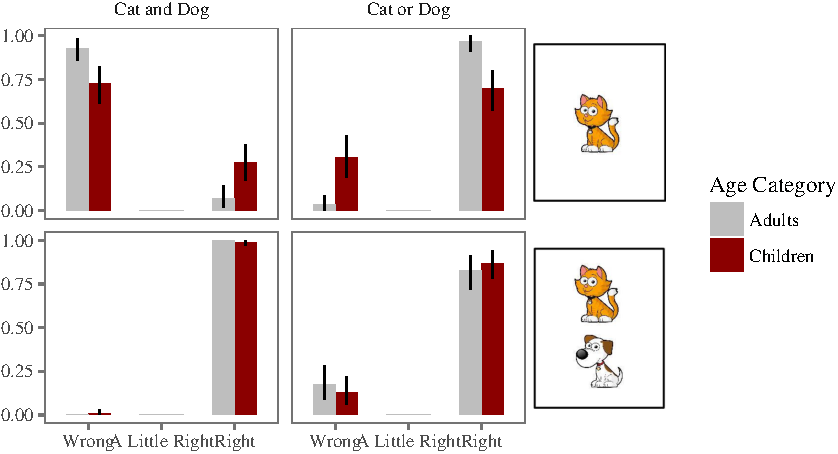
\includegraphics{figs/BinaryPlotComp-1} 

}

\caption{The comparison of the 2AFC judgment task for conjunction and disjunction trials in adults (study 1) and children (study 3).}\label{fig:BinaryPlotComp}
\end{figure}
Finally, there is a small but significant preference in children's
judgments of disjunctive statements for both disjuncts to be true.
Comparing the disjunctive trials with one animal and two animals on the
card, a mixed-effects logistic model with the fixed effect of
disjunction type and the random effect of subjects found that children
had a slight preference for both animals to be on the card (\(b\)= 1.85,
\(se\)= 0.56, \(z\)= 3.32, \(p < 0.001\) ). There was a similar small
trend in children's three-alternative judgments in study 2. While this
was quite small compared to the other effects observed in these studies,
it nevertheless indicated a minor difference between children's and
adults' judgments. I will return to this in more detail in section
\ref{conjunctive} of the General Discussion.

\subsubsection{Open-ended Feedback}\label{open-ended-feedback}
\begin{figure}[h]

{\centering 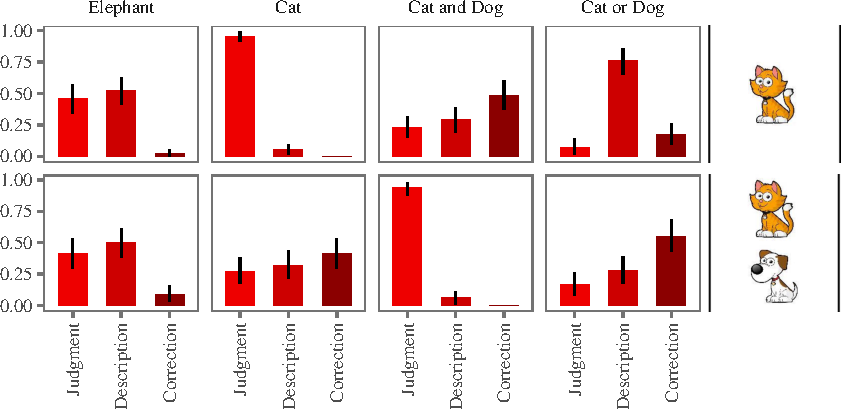
\includegraphics{figs/feedbackStudy3-1} 

}

\caption{Children's Open-ended Feedback. Error bars represent 95\% confidence intervals.}\label{fig:feedbackStudy3}
\end{figure}
Figure \ref{fig:feedbackStudy3} shows the distribution of children's
feedback to the puppet in Study 3. (See table \ref{tab:feedbackCat} for
the definitions and examples of feedback categories. There were no
``None'' responses in this study since the experimenter explicitly asked
children to provide feedback to the puppet. The distribution of the
responses in the other three categories (Judgment, Description, and
Correction) revealed a successful replication of Study 2.

Children's feedback showed four main patterns. First when the puppet
guessed an animal not on the card (e.g.~elephant), there is a split
pattern between negative judgments like ``no!'' and simple descriptions
of what was on the card, e.g. ``cat!''. Children provided no corrections
on such trials. Second, almost all children responded with positive
judgments like ``yes'' when the puppet's guess accurately matched what
was on the card. This was the case in trials where there was only one
animal on the card (e.g.~cat) and the puppet mentioned it, and trials
where there were two animals and the puppet mentioned both with a
conjunction (e.g.~cat and dog). Third, children provided the highest
number of corrective feedback in trials where the guess was either false
or infelicitous. These included three trial types: (a) the ones where
there were two animals on the card but the puppet only guessed one
(e.g.~cat); (b) the ones where the puppet guessed two animals with
conjunction (e.g.~cat and dog) but only one of them was on the card; and
(c) the ones where there were two animals and the puppet guessed both
but used a disjunction (e.g.~cat or dog). The fourth general pattern was
unique to disjunctive trials with only one animal on the card. In such
cases, almost all children simply named the animal on the card (e.g.
``Cat!'').
\begin{figure}[t]

{\centering 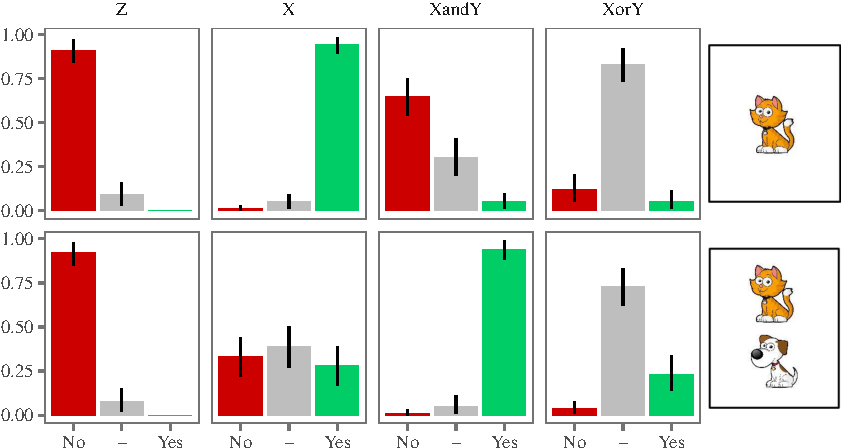
\includegraphics{figs/study3JudgmentPlot-1} 

}

\caption{Children's open-ended feedback to the puppet's guesses.}\label{fig:study3JudgmentPlot}
\end{figure}
Figure \ref{fig:study3JudgmentPlot} breaks down children's open-ended
feedback based on whether children said ``yes'', ``no'', or said
something else. Responses that were not yes/no judgments are grouped in
a middle category shown with a dash. The goal here is to compare
children's open-ended judgments with their forced choice judgments shown
in figure \ref{fig:Study3tvjtPlot}. Children's open-ended judgments and
their forced choice judgments in study 3 show similar patterns for all
types of guesses except for disjunctive ones. In trials that the puppet
guessed using ``or'', the vast majority of children refused to provide a
yes/no judgment when they were not forced to. Instead, they described
the animal on the card or provided corrections to the puppet's
infelicitous disjunctive guess.

One way to interpret these results is that disjunctive guesses (with at
least one disjunct true) are considered neither right nor wrong by
almost all children. When children were forced to provide wrong-right
responses in the experimental context, some may conformed to the adult
patterns of judgment and some did not. However, it is possible that such
deviations from adult judgments do not reflect differences in the
comprehension of disjunction, but rather differences in how children map
their adult-like comprehension onto the notions of ``right'' and
``wrong'' in a forced choice judgment task.
\begin{figure}[t]

{\centering 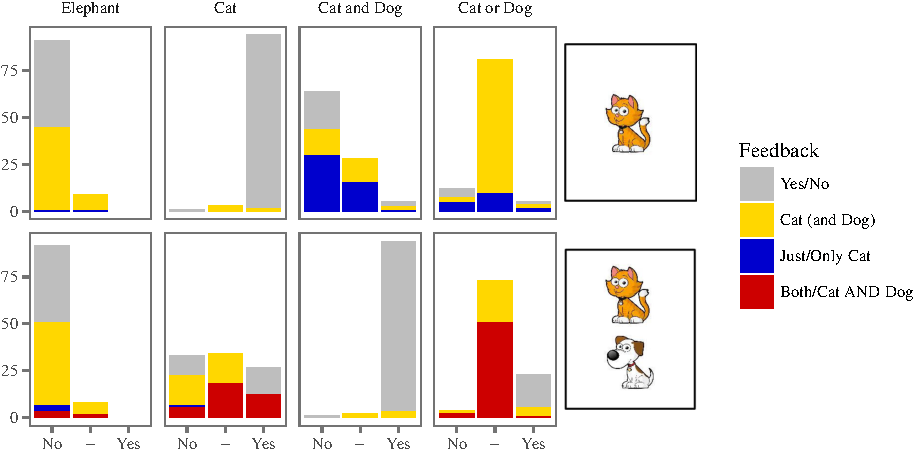
\includegraphics{figs/feedbackFillPlot-1} 

}

\caption{Children's open-ended feedback. The x-axis shows whether children said yes or no and the color fill shows what children said other than yes/no.}\label{fig:feedbackFillPlot}
\end{figure}
Figure \ref{fig:feedbackFillPlot} is similar to figure
\ref{fig:study3JudgmentPlot} but it uses color-fill to show what
children said in addition to yes or no. The gray color represents the
trials where children only said yes/no and nothing else. The yellow-fill
represents descriptions where children mentioned the animal on the card
(i.e. ``cat!''). The blue fill represents children's corrective feedback
that used the exclusive focus particles \emph{just} or \emph{only} (i.e.
``just a cat!''). Such a corrective feedback suggests that the guess
included an animal that did not belong and should have been excluded.
Finally the red fill represents the inclusive corrective feedback that
emphasized the word \emph{and} or said \emph{both} (i.e. ``both'', ``cat
AND dog''). Such corrective feedback indicated that two animals should
be included.

As shown in the leftmost column, when the puppet mentioned an animal
that was not on the card (e.g.~elephant), children responded with a
simple ``no'' or ``no'' followed by what \textbf{was} on the card
(e.g.~no! elephant!). When there was only one animal on the card and the
puppet mentioned the animal (e.g.~cat), children responded with a simple
``yes''. However, when the card had two animals (e.g.~cat and dog) and
the puppet only mentioned one of them (e.g.~cat), children were likely
to provide inclusive feedback. They said \emph{both} or emphasized
\emph{and}, as in ``cat \textbf{AND} dog''. However, in such trials
children were equally split between saying yes, no, or neither.

In the trials with conjunctive and disjunctive guesses, when there was
only one animal on the card (e.g.~cat) and the puppet used a conjunction
(e.g.~cat and dog), children were likely to say a simple ``no'' or say
``no'', followed by ``only/just'' (e.g.~no, just a cat). Some children
did not say ``no'' but did respond with ``only/just''. When the card had
two animals on it and the puppet mentioned both using \emph{and},
children responded with a simple ``yes''. In trials with disjunctive
guesses like ``cat or dog'', children avoided yes/no responses. Instead,
when the card had only one animal, children mentioned that animal. When
the card had both animals, children said \emph{both} or emphasized the
word \emph{and}, as in ``cat \textbf{AND} dog''.
\begin{figure}[t]

{\centering 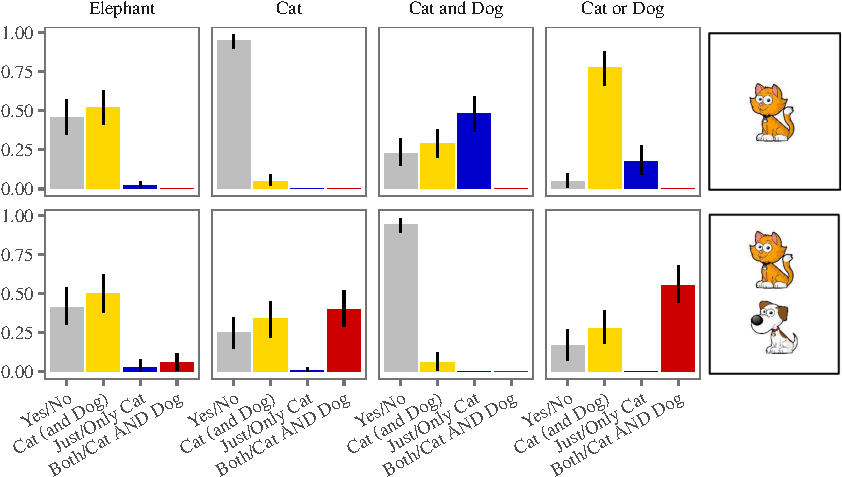
\includegraphics{figs/correctivePlot-1} 

}

\caption{Children's feedback categories in disjunction trials.}\label{fig:correctivePlot}
\end{figure}
Figure \ref{fig:correctivePlot} shows the same feedback data in Figure
\ref{fig:feedbackFillPlot} but uses the x-axis to also show the
proportion of feedback categories other than yes/no judgments. My goal
here was to display the trial types with corrective feedback (blue and
red). These trial types include: (1) conjunction when only one conjunct
is true, (2) disjunction when both disjuncts are true, (3) simple
guesses (e.g. ``there is a cat'') when two animals were on the card.
These trial types involved guesses that are either false or
infelicitous.

Furthermore, the type of corrective feedback children provided matched
the type of mistakes made in the guesses. With conjunctive guesses like
``cat and dog'' when there was only one animal on the card (e.g.~cat),
children provided exclusive corrections (e.g.~just/only a cat),
suggesting that the other animal (e.g.~dog) should have been excluded.
With disjunctive guesses like ``cat or dog'' and simple guesses like
``cat'' when there were two animals on the card, children provided
inclusive feedback, indicating that another animal should have been
included. This is particularly notable in the case of disjunction since
both animals were mentioned, but children still emphasized that the
connective \emph{and} should have been used, or that \emph{both}
mentioned animals were on the card.

\subsection{Discussion}\label{discussion-3}

Study 3 measured children's comprehension of logical connectives by
asking them to judge a puppet's guess in two ways: with open-ended
feedback and with a two-alternative forced choice task. First, I asked
children to say ``yes'' to the puppet if he was right and ``no'' if he
was wrong. However, children could provide any form of feedback they
wanted. Second, I followed children's open-ended feedback with a
two-alternative forced choice question: ``Was the puppet right?'' This
way, I could measure children's comprehension in two different ways in
the same trial. Ideally, both measures should show similar results.
However, the findings were similar for conjunctive guesses, but not
disjunctive ones. Children avoided binary right/wrong feedback with
disjunction and preferred to provide more nuanced feedback when they
could.

The 2AFC responses followed the predicted pattern: conjunctive guesses
with only one conjunct true were considered wrong while those with both
conjuncts true were judged to be right. Disjunctive guesses were judged
right whether one or both disjuncts was true. There was no significant
difference in the 2AFC task between the responses of children and those
of adults in Study 1.

Children's open-ended feedback in Study 3 replicated that in Study 2.
They provided more corrective feedback in false and infelicitous trials
than in true and felicitous ones. The corrective feedback was tailored
to the puppet's mistake. If the puppet used a conjunction when there was
only one animal on the card, children pointed out that the other animal
should have been excluded using the exclusive adverbials \emph{just} and
\emph{only}. If the puppet used a disjunction when both animals were on
the card, children stressed \emph{and} or \emph{both}, implying that
both animals should be included.

While the 2AFC results suggested that children take no issue with
disjunctive guesses when both disjuncts are true, the analysis of their
corrective feedback showed that they provide appropriate corrections in
such cases and emphasize that the connective \emph{and} would have been
a better guess. Taking both measures together, I conclude that even
though children are aware of the problem with such guesses, they do not
consider them \emph{wrong}. These results are similar to what I reported
for adults in Study 1.

\section{General Discussion}\label{general-discussion}

I reported three studies on adults and four-year-olds' comprehension of
the logical connectives \emph{and} and \emph{or}. The first study used
two- and three-alternative forced choice judgment tasks with adults. In
the 2AFC task, adult interpretations closely matched the semantic
accounts of \emph{and} and \emph{or} as conjunction and inclusive
disjunction. The judgments did not register robust signs of pragmatic
infelicities. However, the 3AFC judgment task, showed signs of pragmatic
infelicities, especially in disjunctive guesses with true disjuncts.
When both disjuncts were true, participants were more likely to choose
``kinda right'' rather than ``right''.

The second study used a 3AFC judgment task with four-year-old children.
It also included an exploratory analysis of children's open-ended verbal
feedback to the puppet in the experimental setting. Children's
interpretations were similar to those of adults in the 3AFC task and
only differed for pragmatically infelicitous disjunctions. When both
disjuncts were true, adults tended to judge disjunctive guesses as
``kinda right''. This was evidence for the pragmatic infelicity of such
guesses. While, children judged such disjunctive statement as ``right'',
the analysis of their open-ended feedback showed that they took issue
with such statements as well, and provided appropriate corrective
feedback.

In the third study, I focused on eliciting open-ended verbal feedback
from children and followed it with a 2AFC task. In the 2AFC task,
children's responses reflected the semantics of connectives as
conjunction and inclusive disjunction. There was no significant
difference between children and adults in the two-alternative judgments.
Since the 2AFC task appeared to be a good indicator of semantic
knowledge, it seemed reasonable to conclude that adults and
four-year-olds displayed similar semantic knowledge of the connectives.
Analysis of the children's open-ended feedback replicated the findings
in study 2. Children provided more corrective feedback in false and
pragmatically infelicitous trials with logical connectives than in
felicitous trials. The comparison of the 2AFC task and children's
open-ended responses shows that children are sensitive to the infelicity
of disjunctions with true disjuncts, even though they consider them to
be ``right'' guesses.

Overall, I did not find major differences between adults' and
four-year-old children's interpretations of logical connectives
\emph{and} and \emph{or} in the context of the guessing game. However,
there were two minor differences. First, I found that in both 2AFC and
3AFC judgment tasks, children showed a small preference for disjunctions
with both disjuncts true rather than only one. Adults on the other hand
showed the opposite pattern: they preferred disjuncts with only one
disjunct true. Second, in both 2AFC and 3AFC judgment tasks, children
rated disjunctions with both disjuncts true higher than adults. That is,
they considered utterances like ``there is a cat or a dog'' when both
animals were on the card ``right'' more often than adults. Here I
discuss these two differences and their potential causes in more detail.

\subsection{Preference for True Disjuncts}\label{conjunctive}

First for some children, there was a small preference for both disjuncts
being true, compared to only one. This effect is similar in kind but not
magnitude, to an effect that Singh et al. (2016) and L. Tieu et al.
(2016) reported. In my study this effect is quite small while Singh et
al. (2016) and L. Tieu et al. (2016) seem to have found bigger effects.
Based on this, Singh et al. (2016) proposed that many children at this
age-range have a pragmatically driven conjunctive interpretation of
disjunction. In short, due to a non-adult like alternative set to the
connective \emph{or}, children strengthen a disjunctive statement
pragmatically and derive a conjunction. The studies reported here
provide no support for this proposal. In both 2AFC and 3AFC judgments,
children clearly differentiated between disjunctive and conjunctive
guesses. Furthermore, analysis of children's open-ended feedback showed
distinctly different response patterns for conjunction and disjunction.
More importantly, the open-ended feedback to disjunctive guesses showed
the opposite pattern to that predicted by the conjunctive hypothesis.
Children took issue with disjunctions that had both disjuncts true and
provided more corrective feedback in such cases. Therefore, Singh et al.
(2016) and L. Tieu et al. (2016) findings appear to be a product of
forced choice tasks rather than a real reflection of children's
comprehension of connectives.

However, even assuming that this small preference for true disjuncts is
not due to the measurement method, it can be accounted for by several
other hypotheses that have not been successfully ruled out yet. First,
the conjunctive interpretation may not be due to a faulty pragmatic
computation, but rather a default conjunctive interpretation when the
connective is not properly heard/understood or is unknown. To check this
hypothesis, it may be possible to test children's comprehension of novel
or noisy connectives. A novel coordination like \emph{cat dax dog} with
\emph{dax} as a nonce connective may be interpreted as a conjunction.
Such results would suggest that in studies with high cognitive demand,
children may default to a conjunctive interpretation if they miss the
relevant connective. Second, the conjunctive preference may be due to
some children's preference for the linguistic labels to match the
animals on the card (or more generally linguistic description and state
of the world). This hypothesis is consistent with the results in the
other trial type that had mismatch in the number of animals and the
guess while the guess was technically true: simple guesses (e.g.~there
is a cat) when two animal (e.g.~cat and dog) were present on the card.
Children were equally split between ``wrong'' and ``right'' in their
judgments while adults considered such guesses as ``right''. In light of
these alternative explanations, I are hesitant to attribute this small
preference to a pragmatically driven conjunctive interpretation of
disjunction.

\subsection{Lack of Infelcity with True
Disjuncts}\label{lack-of-infelcity-with-true-disjuncts}

The second difference between adults and children emerged in the 3AFC
judgment task: in disjunctive trials (e.g. ``cat or dog'') with two
animals (e.g.~cat and dog), adults were more likely to choose ``kinda
right'' than children were. Children mostly chose ``right''. This
response pattern is often taken to mean that children found no
infelicity with such disjunctions or that they did not ``derive an
exclusivity implicature''. This lack of infelicity/implicature is
consistent with the generalization that children are more likely than
adults to interpret scalar terms literally, and that children do not
compute implicatures or judge infelicity to the same \textbf{rate} that
adults do (Pouscoulous \& Noveck, 2009, Katsos (2014)). But why is that?

There have been three major proposals to account for children's low rate
of implicatures: 1. processing (Reinhart, 2004, Pouscoulous, Noveck,
Politzer, \& Bastide (2007)) 2. non-adult-like lexical entry (Barner et
al. (2011), Horowitz, Schneider, \& Frank (2017)) and 3. pragmatic
tolerance (Katsos \& Bishop, 2011). Here I show that none of these
accounts provide a satisfactory explanation of the results in this
study.

\textbf{1. Processing} First, the processing accounts locate the problem
in children's processing capacities such as working memory. They suggest
that pragmatic computations are cognitively taxing and children lack the
appropriate processing resources to carry them out appropriately. A
prediction of processing accounts (at least in their current format) is
that children will show reduced implicature computations for all types
of implicatures - scalar or ad-hoc. This prediction was not borne out in
my experimental results. In Study 3, children were much more likely than
adults to call a simple guess (e.g. ``cat'') ``wrong'' in the 2AFC task
if there were two animals on the card (e.g. ``cat and dog''). Processing
accounts do not predict that children would derive more implicatures
than adults but this is what I found for the traditional interpretation
of the judgment task.

\textbf{2. Non-adult Like Lexicon} Several proposals blame the structure
of the child's lexicon for the alleged failure in deriving
implicatures/infelicity. The assumption is that the child's lexical
entry for scalar items must include three elements for successful
derivation: 1. the semantics of the weak term (e.g. \emph{some},
\emph{or}) 2. the semantics of the strong term (e.g.
\emph{all},\emph{and}); and possibly 3. a scale that recognizes the
stronger term as an alternative to the weaker one (e.g.
\textless{}\emph{some}, \emph{all}\textgreater{}, \textless{}\emph{or},
\emph{and}\textgreater{}). Each of these elements have been pinpointed
as the source of the problem in previous studies (Horowitz et al., 2017,
Katsos \& Bishop (2011), Barner et al. (2011)). However none of them
seem to apply to the results reported here.

If children in this study lack the semantics of the connective
\emph{or}, I can expect them to either perform at chance or default to a
conjunctive interpretation. Neither prediction is borne out in study 2
and 3. Furthermore, children's free-form linguistic feedback suggests
good understanding of disjunction. So this explanation seems unlikely.
The problem cannot be that children do not know the meaning of
\emph{and} either. Children's performances in both study 2 and 3 for
conjunction trials show that they understand its meaning very well.
Finally, while it is possible that children lacked the appropriate
lexical scale and could not access the stronger alternative, this
explanation cannot be the whole story. Several children in both study 2
and 3 stressed the word \emph{and} suggesting that the puppet should
have used the stronger term instead. However, they judged the puppet's
guess as ``right''. If children could not access the stronger term, they
could not mention it in their feedback either.

\textbf{3. Pragmatic Tolerance} Katsos \& Bishop (2011) suggested that
children tend to tolerate pragmatic infelicities more than adults. They
showed that when children are provided with a 2AFC judgment task, they
tolerate the infelicity of \emph{some} when \emph{all} applies but when
they are presented with a 3AFC task they choose the middle option and
report this infelicity. As in a processing account, the pragmatic
tolerance account predicts that scalar and ad-hoc implicatures will be
similarly affected. However, I did not find results similar to those of
Katsos \& Bishop (2011). When children were presented with a 3AFC task,
they chose the highest reward (and not the middle option) for uses of
\emph{or} when \emph{and} applied. Second, and more importantly, I found
different patterns for ad-hoc and scalar implicatures as mentioned
before. This is not predicted by the tolerance account unless children
are assumed to be more tolerant towards violations of scalar
implicatures than they are towards ad-hoc ones. While tolerance may not
be the source of the problem here, I believe that a number of
discussions including those of Katsos \& Bishop (2011) and later Katsos
(2014) point to an important factor: the role of measurement in
estimates of children's pragmatic capacity.

Several observations in the current studies here provide support for the
hypothesis that methodological issues, and more specifically issues of
measurement contribute to the differences found between adults and
children in pragmatic capacity. First, Study 1 showed that even for
adults, the estimates of adult infelicity rates may differ based on the
number of alternatives in the forced choice task. A 2AFC task tends to
underestimate adults' rate of response to pragmatic infelicity. Second,
children's open-ended linguistic feedback in the experimental context
better reflected their sensitivity to pragmatic nuances than the
forced-choice judgment tasks. Third, children showed a higher rate of
infelicity judgments for cases of ad-hoc implicatures (simple guesses
with two animals on the card) than adults did. While a difference in
sensitivity to ad-hoc vs.~scalar implicatures has been reported and
argued for before (Horowitz et al., 2017; Stiller, Goodman, \& Frank,
2015), a higher sensitivity than adults is not predicted by any of the
current accounts.

In order to better understand the differences between adults and
children's pragmatic capacities, it is necessary to have a good
understanding of how measurements affect estimates of adults and
children's performance in the experimental tasks. Children may be no
more capable of making exhaustive inferences than adults and not less
capable of making scalar inferences either. They may simply have a
different construal of the wrong-right scale and of what the
forced-choice task is about. The concepts ``right'' and ``wrong'' are as
much subject to developmental change and differences between adults and
children as are scalar items in general. It is reasonable to assume that
children's understanding of what constitutes as ``right'' or ``wrong''
does not conform to that of adults. However, it remains to be
established what these differences are and how they affect the estimates
of children's pragmatic abilities. It is important to point out that
such issues of measurement could be the culprit behind both children's
seemingly slight preference for true disjuncts explained earlier and for
their lack of infelicity when both disjuncts are true.

\textbf{A General Approach for Measuring Implicature/Infelicity Rate}

Methodological issues are nothing new in studies of children's semantic
and pragmatic development. Developing the best measures of children's
linguistic capacities has always been a major concern for researchers in
the field. My goal here is to propose some future steps that can address
the methodological concerns in children's pragmatic development.

As Pouscoulous \& Noveck (2009) and Katsos (2014) have suggested, the
central issue is \textbf{the rate} at which children and adults manifest
pragmatic reasoning in the experimental setting. No one doubts
children's capacity to perform such computations. At issue is the extent
to which children and adults compute implicatures. And the claim is that
children perform such computations less often than adults; or that
children do not perform such computations when adults normally would. In
the previous section, I discussed factors that can cause this difference
including processing demands, the structure of the lexicon, tolerance,
as well as issues of measuring adults and children's comprehension. As
Katsos (2014) pointed out, it seems reasonable to assume that all these
factors play some part here. What matters is the degree to which each
contributes to the outcome.
\begin{figure}[t]

{\centering 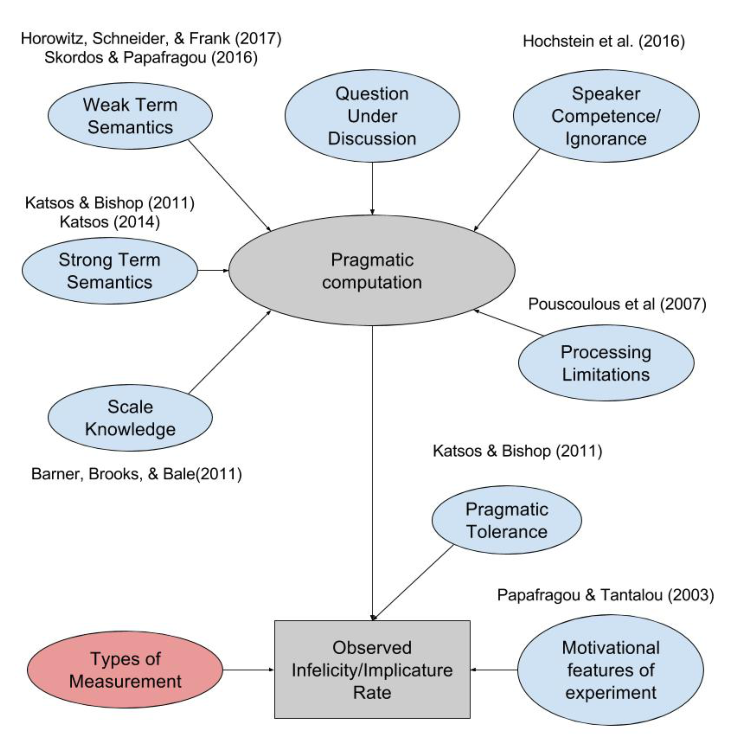
\includegraphics{figs/implicatureGraph-1} 

}

\caption{Factors that coul affect pragmatic computations and the estimates of these computations in the experimental settings.}\label{fig:implicatureGraph}
\end{figure}
Figure \ref{fig:implicatureGraph} shows the factors that affect
pragmatic computations as well as the observations of the rate of
pragmatic computations in an experiment. First it is important to
distinguish between factors that affect pragmatic computations and those
that affect the observed rate in the experimental setting. As I showed
in experiment 1, given the number of alternatives in the forced choice
task (2AFC vs.~3AFC), I may get different estimates of adults'
infelicity judgments, yet it is unreasonable to assume that there is a
difference in adults' pragmatic capacities in these two tasks. A similar
situation exists when I compare children's forced choice measures of
infelicity and their open-ended feedback. In disjunctive trials where
both disjuncts are true, the forced choice tasks show no sign of
infelicity while the open ended responses show that children are
sensitive to the infelicity of disjunction when a conjunction would have
been more appropriate.

\section{Conclusion}\label{conclusion}

To conclude, I showed that children and adults do not differ
substantially in their \textbf{semantic} knowledge of the logical
connectives. The results were highly consistent with the current
accounts that posit the semantics of \emph{and} as logical conjunction
and \emph{or} as logical (inclusive) disjunction. With respect to
pragmatic knowledge, the three-alternative forced choice judgment task
showed that adults are sensitive to the infelicity of disjunctive
statements when both disjuncts are true. I showed that while the
three-alternative judgment task failed to register such a sensitivity
for children, my systematic analysis of children's verbal open-ended
feedback showed that children are sensitive to pragmatic infelicities
and can provide appropriate corrections to infelicitous utterances with
logical connectives.

\chapter{Parents' and Children's Production of
Disjunction}\label{corpus}

\section{Introduction}\label{introduction-3}

This chapter presents two studies on parents and children's production
of \emph{and} and \emph{or}. The first study investigates the frequency
of \emph{and} and \emph{or} in parents and children's speech to answer
two questions: 1. at what age do children start to produce \emph{and}
and \emph{or}. 2. do children reach their parent's level of production
for these words? and if they do at what age? The second study explores
the frequency of different interpretations \emph{and} and \emph{or} have
in child-directed speech. This study seeks to answer the following two
questions: 1. What are the most frequent interpretations of \emph{and}
and \emph{or} in child-directed speech? 2. What are reliable cues that
can help children interpret and acquire the meanings of \emph{and} and
\emph{or}?

\section{\texorpdfstring{Study 1: \emph{and} and \emph{or} in parents'
and children's
speech}{Study 1: and and or in parents' and children's speech}}\label{study-1-and-and-or-in-parents-and-childrens-speech}

This study investigates the production of \emph{and} \& \emph{or} by
children and their parents in an online collection of corpora. The goal
is to understand the overall frequencies of these items and investigate
the developmental trends in children's productions. After describing the
study methods in section \ref{study1methods}, I investigate some
important properties of the corpora such as their word density for
parents and children at different ages as well as the frequency of
different utterance types in the speech of parents and children. I
explain that function words are sensitive to the distribution of
utterance types or more broadly speech acts or constructions with
particular communicative functions. Therefore, it is important for
developmental studies on the production of function words to investigate
their frequencies within different utterance types, speech acts, or
constructions with specific communicative functions. In section
\ref{study1results}, I first look at the overall and monthly relative
frequencies of \emph{and} and \emph{or} in the speech of parents and
children. Then, I use utterance type as a proxy for speech acts and
investigate the relative frequencies of these connectives within
declaratives and questions. I summarize the main results and important
conclusions of the study in section \ref{study1discussion}.

\subsection{Methods}\label{study1methods}

For samples of parents' and children's speech, this study used the
online database \href{childes-db.stanford.edu}{childes-db R} and its
associated R programming package \texttt{childesr} (Sanchez et al., in
prep). Childes-db is an online interface to the child language
components of \href{https://talkbank.org/}{TalkBank}, namely
\href{https://childes.talkbank.org/}{CHILDES} (MacWhinney, 2000) and
\href{https://phonbank.talkbank.org/}{PhonBank}. Two collections of
corpora were selected: English-North America and English-UK. All word
tokens were tagged for the following information: 1. The speaker role
(mother, father, child), 2. the age of the child when the word was
produced, 3. the type of the utterance the word appeared in
(declarative, question, imperative, other), and 4. whether the word was
``and'', ``or'', or some ``other'' word.
\begin{figure}[tb]

{\centering 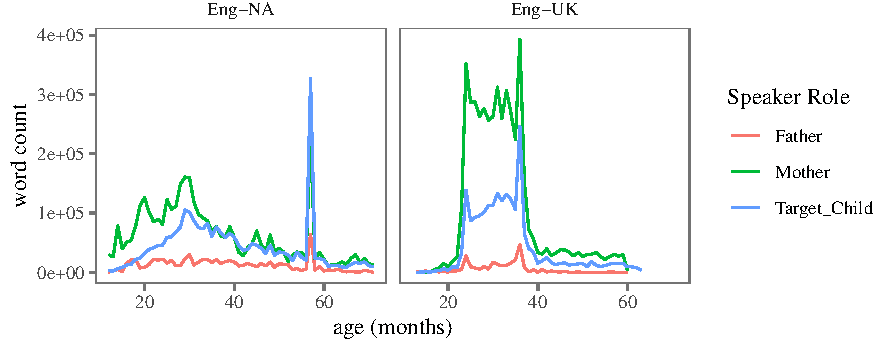
\includegraphics{figs/corpusDensityPlot-1} 

}

\caption{Word frequency in the North America and UK corpora of CHILDES.}\label{fig:corpusDensityPlot}
\end{figure}
\begin{figure}[tb]

{\centering 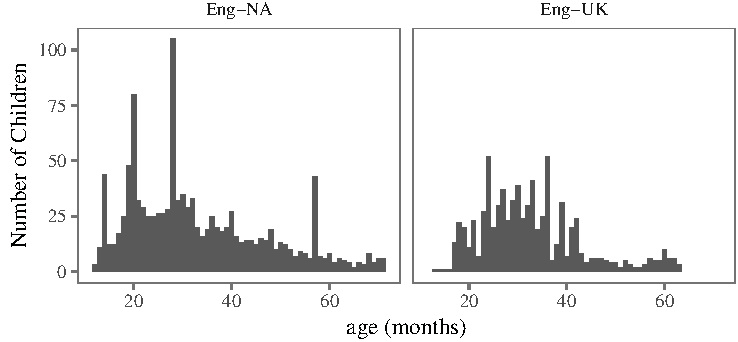
\includegraphics{figs/childDensityPlot-1} 

}

\caption{The number of children represented at different ages in the North America and UK corpora in CHILDES.}\label{fig:childDensityPlot}
\end{figure}
\subsubsection{Exclusion Criteria}\label{exclusion-criteria}

First, observations (tokens) that were coded as unintelligible were
excluded (N = 290119). Second, observations that had missing information
on children's age were excluded (N = 1042478). Third, observations
outside the age range of 1 to 6 years were excluded (N = 686870). This
exclusion was mainly because there was not much data outside this age
range. Figure \ref{fig:ageDistPlot} shows the distribution of
transcripts based on the age of the child at recording time. The mean
age is shown with a red vertical line (Mean Age = 3.73, SD = 2.21). The
collection contained the speech of 504 children and their parents after
the exclusions.

\subsubsection{Procedure}\label{procedure}

Each token was marked for the utterance type that the token appeared in.
This study grouped utterance types into four main categories:
``declarative'', ``question'', ``imperative'', and ``other''. Utterance
type categorization followed the convention used in the
\href{https://talkbank.org/manuals/CHAT.html\#_Toc486414422}{TalkBank
manual}. The utterance types are similar to sentence types (declarative,
interrogative, imparative) with one exception: the category ``question''
consists of interrogatives as well as rising declaratives
(i.e.~declaratives with rising question intonation). In the transcripts,
declaratives are marked with a period, questions with a question mark,
and imperatives with an exclamation mark. It is important to note that
The manual also provides
\href{https://talkbank.org/manuals/CHAT.html\#_Toc486414431}{terminators
for special-type utterances}. Among the special type utterances, this
study included the following in the category ``questions'': trailing off
of a question, question with exclamation, interruption of a question,
and self-interrupted question. The category imperatives also included
``emphatic imperatives''. The rest of the special type utterances such
as ``interruptions'' and ``trailing off'' were included in the category
``other''.
\begin{figure}
\centering
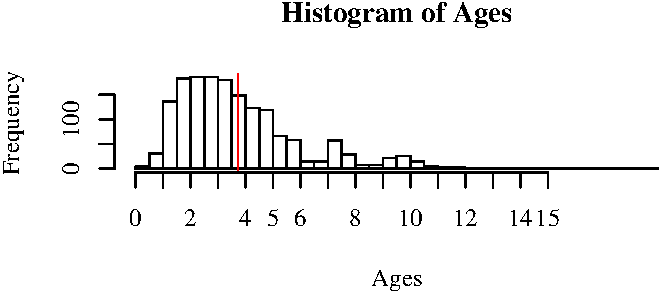
\includegraphics{figs/ageDistPlot-1.pdf}
\caption{\label{fig:ageDistPlot}Distribution of children's ages at recording
times. Mean age is shown using a red vertical line.}
\end{figure}
\subsection{Properties of the CHILDES
Corpora}\label{properties-of-the-childes-corpora}

In this section, I report some results on the distribution of words and
utterances among the speakers in our collection of corpora. The
collection contained 14159609 words. Table (\ref{tab:countTable}) shows
the total number of \emph{and}'s, \emph{or}'s, and words in the speech
of children, fathers, and mothers. The collection contains 8.8 times
more words for mothers compared to fathers and 1.8 more words for
mothers compared to children. Therefore, the collection is a better
representative of the mother-child interactions than father-child
interactions. Compared to \emph{or}, the word \emph{and} is 10.8 times
more likely in the speech of mothers, 9.2 times more likely in the
speech of fathers, and 30.3 times more likely in the speech of children.
Overall, \emph{and} is 13.35 times more liklely than \emph{or} in this
collection which is close to the rate reported by Morris (2008). He
extracted 5,994 instances of \emph{and} and 465 instances of \emph{or}
and found that overall, \emph{and} was 12.89 times more frequent than
\emph{or} in child-parent interactions.
\begin{table}

\caption{\label{tab:countTable}Number of and's, or's, and the total number of words in the speech of children and their parents in English-North America and English-UK collections after exclusions.}
\centering
\begin{tabular}[t]{l|r|r|r}
\hline
Speaker Role & and & or & total\\
\hline
Father & 15,488 & 1,683 & 967,075\\
\hline
Mother & 153,781 & 14,288 & 8,511,478\\
\hline
Target\_Child & 78,443 & 2,590 & 4,681,056\\
\hline
\end{tabular}
\end{table}
Figure \ref{fig:wordsByAge} shows the number of words spoken by parents
and children at each month of the child's development. The words in the
collection are not distributed uniformly and there is a high
concentration of data between the ages of 20 and 40 months (around 2 to
3 years of age). There is also a high concentration around 60 months (5
years of age). The speech of fathers shows a relatively low word-count
across all ages. Therefore, in our analyses we should be more cautious
in drawing conclusions on the speech of fathers generally, and the
speech of mothers and children after age 5.
\begin{figure}[tb]

{\centering 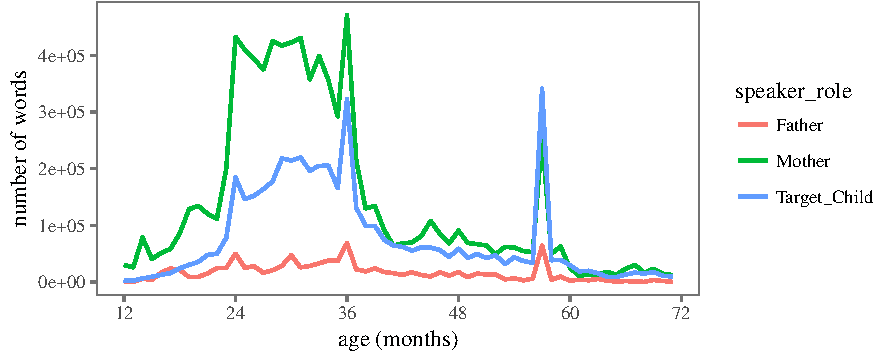
\includegraphics{figs/wordsByAge-1} 

}

\caption{The number of words in the corpora for parents and children in each month of children's development.}\label{fig:wordsByAge}
\end{figure}
The distribution of function words is sensitive to the type of utterance
or more broadly the type of speech act produced by speakers. For
example, question particles may appear more frequently in questions than
other types of utterance. Therefore, it is important to check the
distribution of speech acts in corpora when studying different function
words. Since it is hard to classify and quantify speech acts
automatically, here I use utterance type as a proxy for speech acts. I
investigate the distribution of declaratives, questions, and imperatives
in our collection of corpora on child-parent interactions. Figure
\ref{fig:totalUtteranceTypePlot} shows the distribution of different
utterance types in the speech of parents and children. Overall, most
utterances are either declaratives or questions, and there are more
declaratives than questions in our collection. While mothers and fathers
show similar proportions of declaratives and questions in their speech,
children produce a lower proportion of questions and higher proportion
of declaratives than their parents.
\begin{figure}[tb]

{\centering 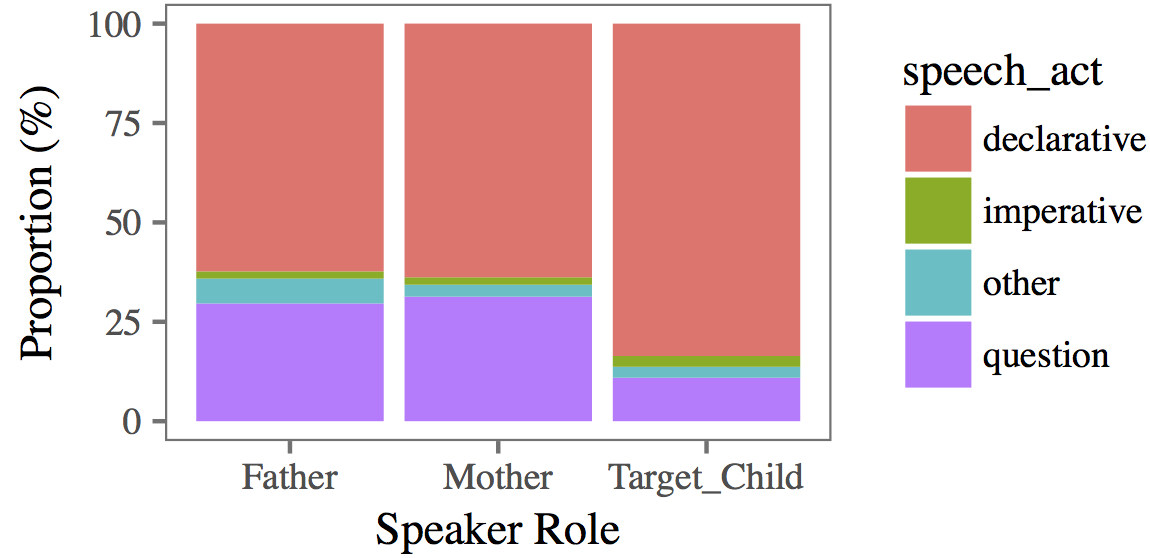
\includegraphics{figs/totalUtteranceTypePlot-1} 

}

\caption{The proportion of declaratives and questions in children's and parents' utterances.}\label{fig:totalUtteranceTypePlot}
\end{figure}
Figure \ref{fig:utteranceTypeByAgePlot} shows the developmental trend of
declaratives and questions between the ages of one and six. Children
start with only producing declaratives and add non-declarative
utterances to their repertoire gradually until they get closer to the
parents' rate around the age six. They also start with very few
questions and increase the number of questions they ask gradually. It is
important to note that the rate of declarative and questions in
children's speech does not reach the adult rate. These two figures show
that parent-child interactions are asymmetric. Parents ask more
questions and children produce more declaratives. This asymmetry also
interacts with age: the speech of younger children has a higher
proportion of declaratives than older children.
\begin{figure}
\centering
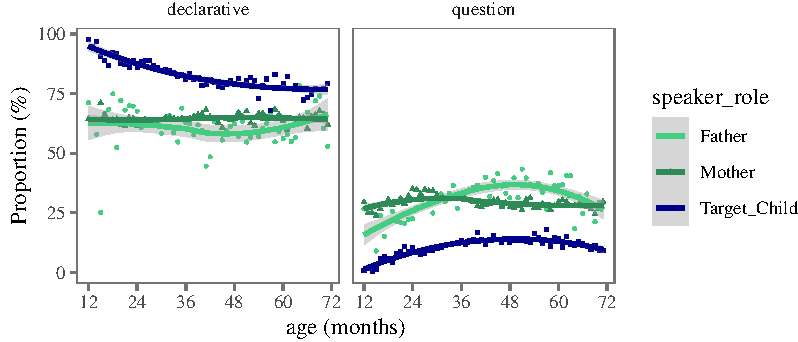
\includegraphics{figs/utteranceTypeByAgePlot-1.pdf}
\caption{\label{fig:utteranceTypeByAgePlot}Proportion of declaratives to
questions in child-parent interactions by age.}
\end{figure}
The frequency of function words such as \emph{and} and \emph{or} may be
affected by such conversational asymmetries if they are more likely to
appear in some utterance types than others. Figure
\ref{fig:CnctPropbySpeechAct} shows the proportion of \emph{and}`s and
\emph{or}'s that appear in different utterance types in parents' and
children's speech. In parents' speech, \emph{and} appears more often in
declaratives (around 60\% in declaratives and 20\% in questions). On the
other hand, \emph{or} appears more often in questions than declaratives,
although this difference is small in mothers. In children's speech, both
\emph{and} and \emph{or} appear most often in declaratives. However,
children have a higher proportion of \emph{or} in questions than
\emph{and} in questions.

The differences in the distribution of utterance types can affect our
interpretation of the corpus data on function words such as \emph{and}
and \emph{or} in three ways. First, since the collection contains more
declaratives than questions, it may reflect the frequency and diversity
of function words like \emph{and} that appear in declaratives better.
Second, since children produce more declaratives and fewer questions
than parents, we may underestimate children's knowledge of function
words like \emph{or} that are frequent in questions. Third, given that
the percentage of questions in the speech of children increases as they
get older, function words like \emph{or} that are more likely to appear
in questions may appear infrequent in the early stages and more frequent
in the later stages of children's development. In other words, function
words like \emph{or} that are common in questions may show a seeming
delay in production which is possibly due to the development of
questions in children's speech. Therefore, in studying children's
productions of function words, it is important to look at their relative
frequencies in different utterance types as well as the overall trends.
This is the approach we pursue in the next section.
\begin{figure}[tb]

{\centering 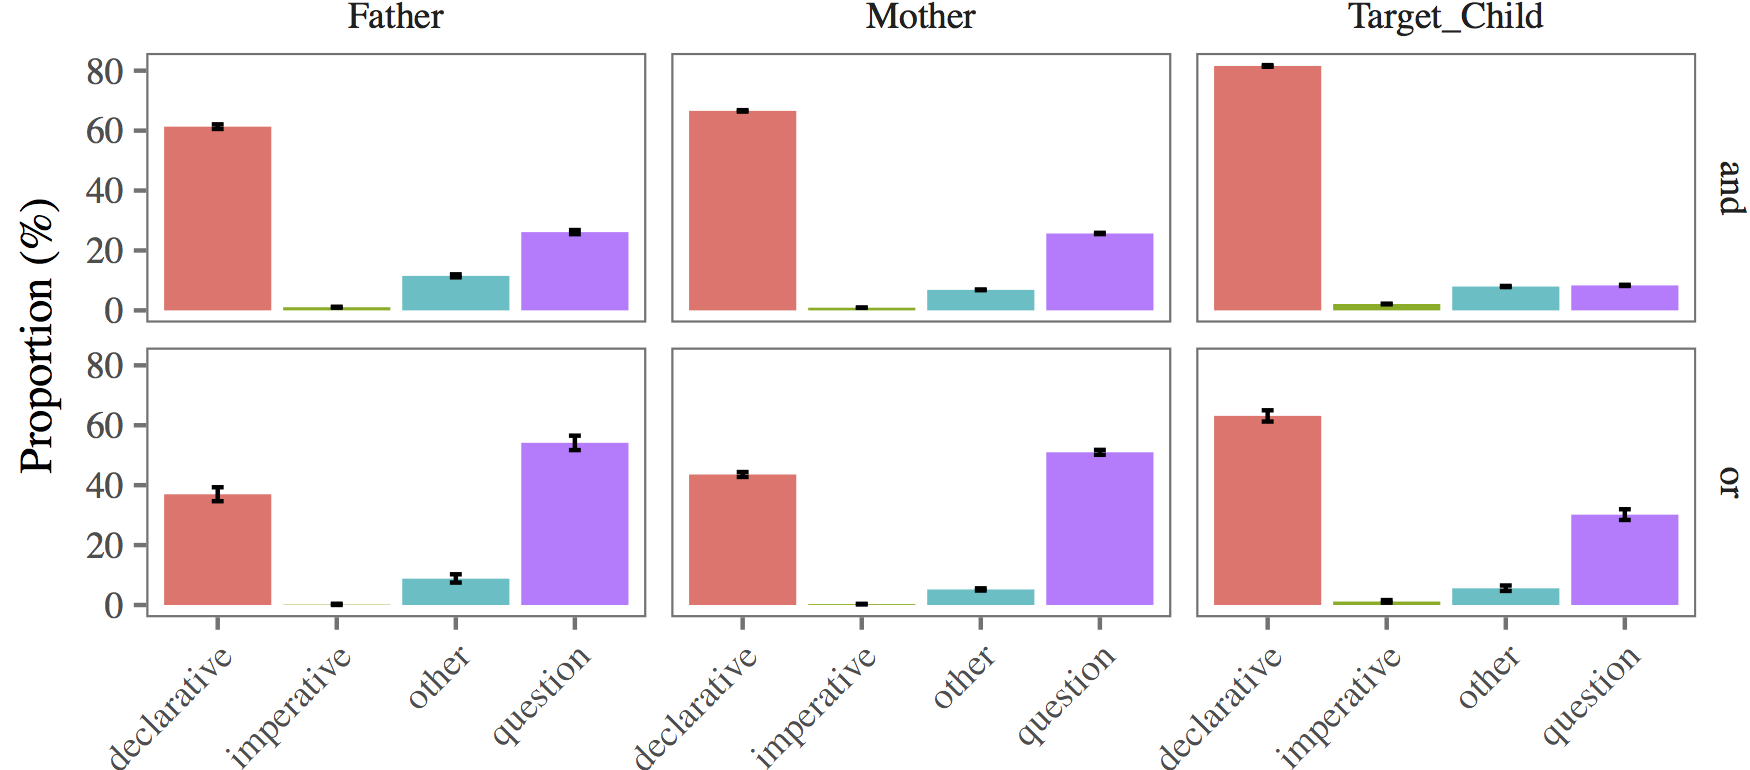
\includegraphics{figs/CnctPropbySpeechAct-1} 

}

\caption{The proportion of and/or in different utterance types in the speech of parents and children.}\label{fig:CnctPropbySpeechAct}
\end{figure}
\subsection{Results}\label{study1results}

First, I consider the overall distribution of \emph{and} and \emph{or}
in our corpora and then look closer at their distributions in different
utterance types. Figure \ref{fig:freqTableBySpeakerPlot} shows the
frequency of \emph{and} and \emph{or} relative to the total number of
words produced by each speaker (i.e.~fathers, mothers, and children).
The y-axes show relative frequency per thousand words. It is also
important to note that the y-axes show different ranges of values for
\emph{and} vs. \emph{or}. This is due to the large difference between
the relative frequencies of these connectives. Overall, \emph{and}
occurs around 15 times per thousand words but \emph{or} only occurs 3
times per 2000 words in the speech of parents and around 1 time every
2000 words in the speech of children. Comparing the relative frequency
of the connectives in parents' and children's speech, we can see that
overall, children and parents produce similar rates of \emph{and} in
their interactions. However, children produce fewer \emph{or}'s than
their parents.
\begin{figure}[tb]

{\centering 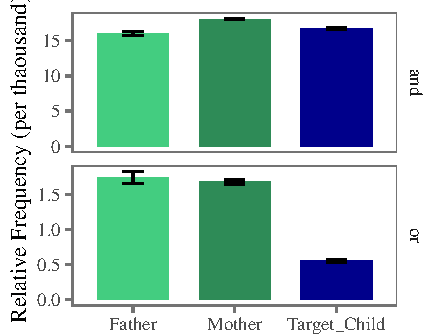
\includegraphics{figs/freqTableBySpeakerPlot-1} 

}

\caption{The relative frequency of and/or in the speech of fathers, mothers, and children. 95\% binomial proportion confidence intervals calculated using Agresti-Coull 's approximate method.}\label{fig:freqTableBySpeakerPlot}
\end{figure}
Next we look at the relative frequencies of \emph{and} and \emph{or} in
parents and children's speech during the course of children's
development. Figure \ref{fig:agePlot} shows the relative frequencies of
\emph{and} and \emph{or} in parents' and children's speech between 12
and 72 months (1-6 years). Production of \emph{and} in parents' speech
seems to be relatively stable and somewhere between 10 to 20
\emph{and}`s per thousand words over the course of children's
development. For children, they start producing \emph{and} between 12
and 24 months, and show a sharp increase in their production until they
reach the parent level between 30 to 36 months of age. Children stay
close to the parents' production level between 36 and 72 months,
possibly surpassing them a bit at 60 months -- although as stated in the
previous section, we should be cautious about patterns after 60 months
due to the small amount of data in this period. For \emph{or}, parents
produce between 1 to 2 \emph{or}'s every thousand words and mothers show
a slight increase in their productions between 12 to 36 months. Children
start producing \emph{or} between 18 to 30 months of age. They show a
steady increase in their productions of \emph{or} until they get close
to 1 \emph{or} per thousand words at 48 months (4 years) and stay at
that level until 72 months (6 years).

Children's productions of \emph{and} and \emph{or} show two main
differences. First, the onset of \emph{or} productions is later than
\emph{and} productions. Children start producing \emph{and} around 1 to
1.5 years old while \emph{or} productions start around 6 months later.
Second, children's \emph{and} production shows a steep rise and reaches
the parent level of production at three-years old. For \emph{or},
however, the rise in children's production level does not reach the
parent level even though it seems to reach a constant level between the
ages of 4 and 6 years. Not reaching the parent level of \emph{or}
production does not necessarily mean that children's understanding of
\emph{or} has not fully developed yet. It can also be due to the nature
of parent-child interactions. For example, since parents ask more
questions than children and \emph{or} appears frequently in questions,
parents may have a higher frequency of \emph{or}. There are two ways of
controlling for this possibility. One is to research children's speech
to peers. Unfortunately such a large database of children's speech to
peers is not currently available for such an analysis. Alternatively, we
can look at the relative frequencies and developmental trends within
utterance types such as declaratives and questions to see if we spot
different developmental trends. This is what I pursue next.
\begin{figure}[tb]

{\centering 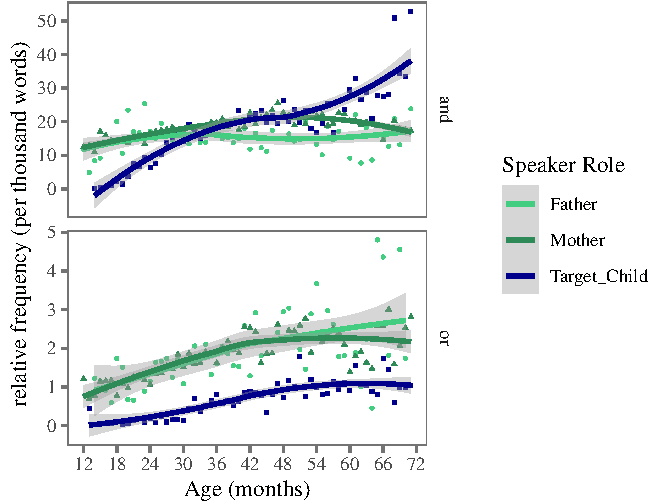
\includegraphics{figs/agePlot-1} 

}

\caption{The monthly relative frequency of and/or in parents and children's speech between the 12 and 72 monts (1-6 years).}\label{fig:agePlot}
\end{figure}
Figure \ref{fig:freqTablebySpeechAct} shows the relative frequency of
\emph{and} and \emph{or} in declaratives, questions, and imperatives.
\emph{and} has the highest relative frequency in declaratives while
\emph{or} has the highest relative frequency in questions. Figure
\ref{fig:ageSpeechActPlot} shows the developmental trends of the
relative frequencies of \emph{and} and \emph{or} in questions and
declaratives. Comparing \emph{and} in declaratives and questions, we see
that the onset of \emph{and} productions are slightly delayed for
questions but in both declaratives and questions, \emph{and} productions
reach the parent level around 36 months (3 years). For \emph{or}, we see
a similar delay in questions compared to declaratives. Children start
producing \emph{or} in declaratives at around 18 months but they start
producing \emph{or} in questions at 24 months. Production of \emph{or}
increases in both declaratives and questions until it seems to reach a
constant rate in declaratives between 48 and 72 months. The relative
frequency of \emph{or} in questions continues to rise until 60 months.
Comparing figures \ref{fig:agePlot} and \ref{fig:ageSpeechActPlot}, we
see that children are closer to the adult rate of production in
declaratives than questions. The large difference between parents and
children's production of \emph{or} in figure \ref{fig:agePlot} may
partly be due to the development of \emph{or} in questions. Overall the
results show that children have a substantial increase in their
productions of \emph{and} and \emph{or} between 1.5 to 4 years of age.
Therefore, it is reasonable to expect that early mappings for the
meaning and usage of these words are developed in this age range.
\begin{figure}[tb]

{\centering 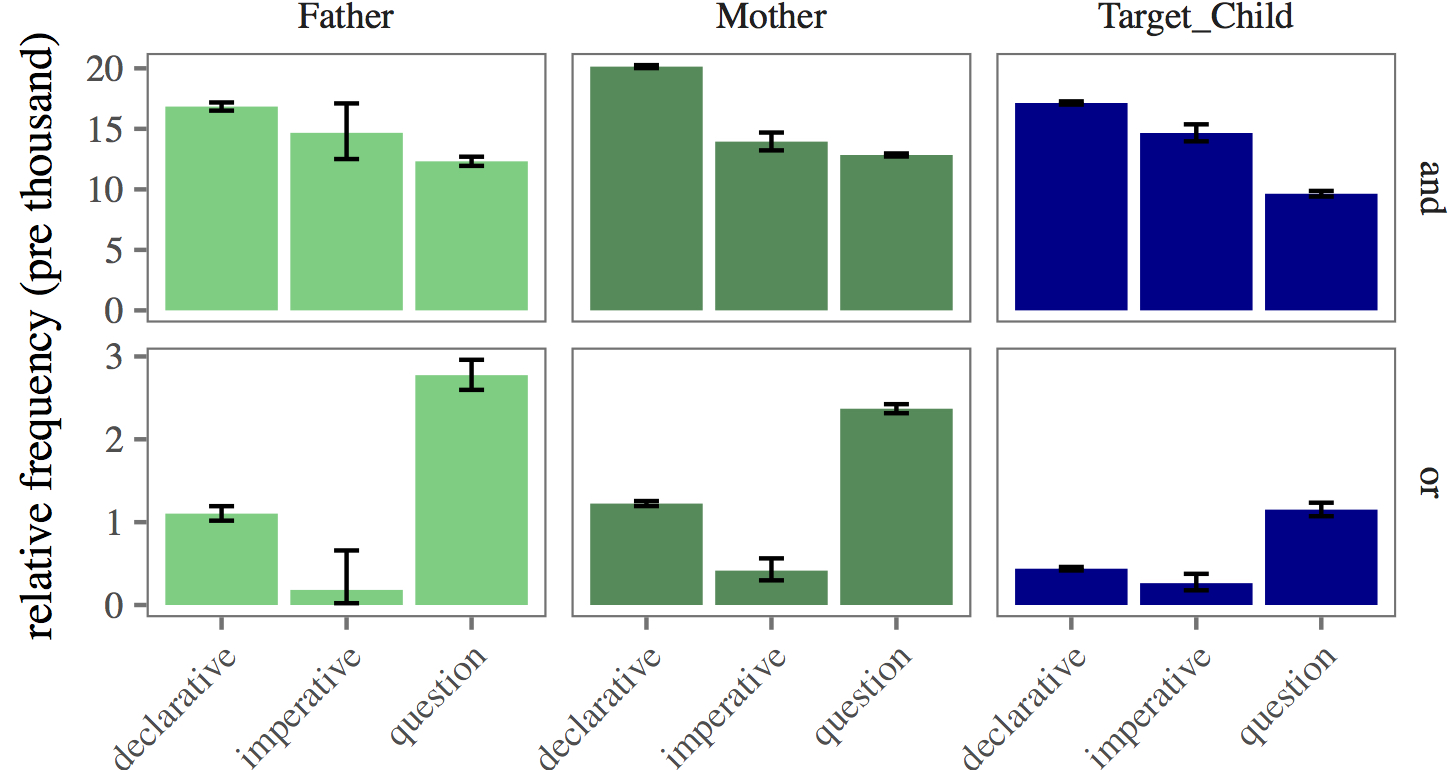
\includegraphics{figs/freqTablebySpeechAct-1} 

}

\caption{Relative frequency of and/or in declaratives, imperatives, and interrogatives for parents and children }\label{fig:freqTablebySpeechAct}
\end{figure}
\begin{figure}[tb]

{\centering 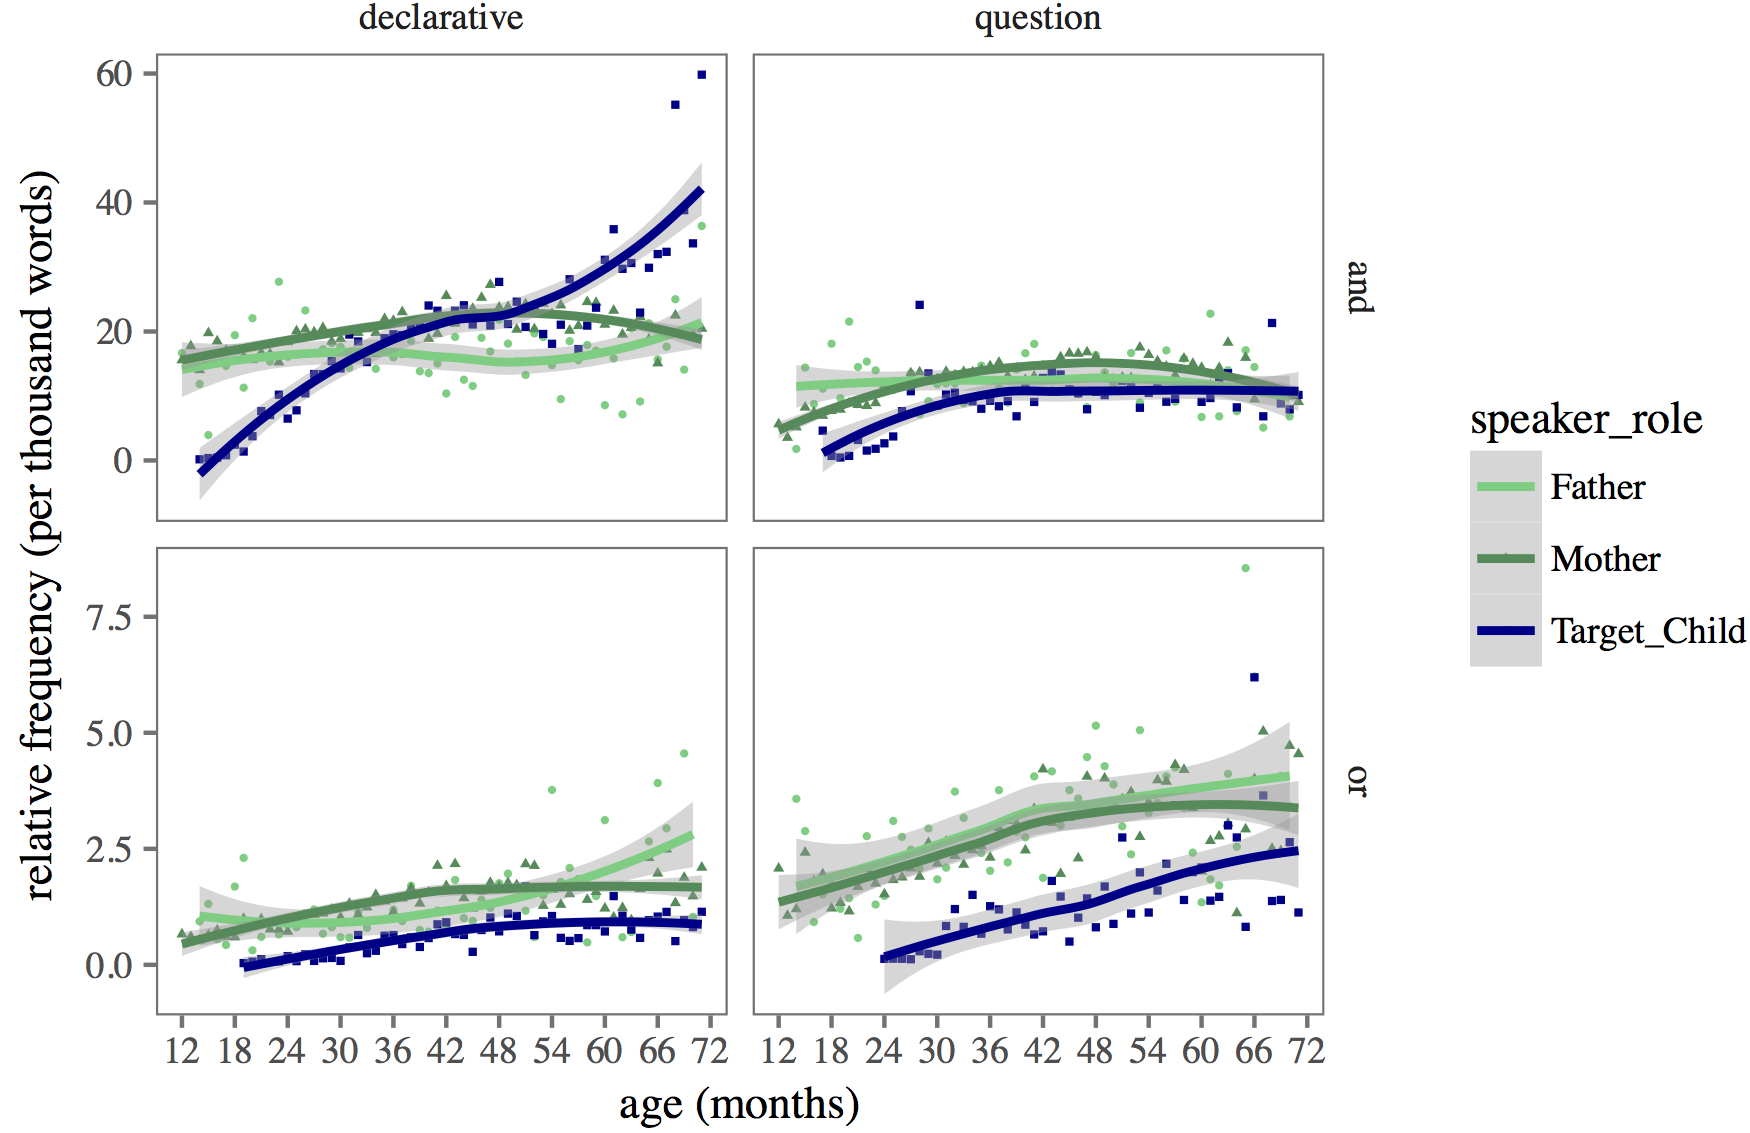
\includegraphics{figs/ageSpeechActPlot-1} 

}

\caption{Relative frequency of and/or in the speech of parents and childern between the child age of one and six years.}\label{fig:ageSpeechActPlot}
\end{figure}
\subsection{Discussion}\label{study1discussion}

The goal of this study was to explore the frequency of \emph{and} and
\emph{or} in parents and children's speech. The study found three
differences. First, it found a difference between the overall frequency
of \emph{and} and \emph{or} in both parents and children. \emph{and} was
about 10 times more frequent than \emph{or} in the speech of parents and
30 times more liklely in the speech of children. Second, the study found
a difference between parents' and children's productions of \emph{or}.
Relative to the total number of words spoken by parents and children
between the ages of 1 and 6 years, both children and parents produce on
average 15 \emph{and}`s every 1000 words. Therefore, children match
parents' rate of \emph{and} production overall. This is not the case for
\emph{or} as parents produce 3 \emph{or}`s every 2000 words and children
only 1 every 2000 words. Third, the study found a developmental
difference between \emph{and} and \emph{or} as well. The study found
that the onset of production is earlier for \emph{and} than \emph{or}.
Looking at the monthly relative frequencies of \emph{and} and \emph{or}
in the speech of parents and children, the study also found that
children reach the parents' level of production for \emph{and} at age 3
while \emph{or} does not reach the parents' level even at age 6.

What causes these production differences? The first difference -- that
\emph{and} is far more frequent than \emph{or} -- is not surprising or
limited to child-directed speech. \emph{and} is useful in a large set of
contexts from conjoining elements of a sentence to connecting discourse
elements or even holding the floor and delaying a conversational turn.
In comparison, \emph{or} seems to have a more limited usage. The second
and the third differences -- namely that children produce fewer
\emph{or}`s than parents, and that they produce \emph{and} and reach
their parents rate earlier than \emph{or} -- can be due to three
factors. First, production of \emph{and} develops and reaches the
parents' rate earlier possibly because it is much more frequent than
\emph{or} in children's input. Previous research suggests that within
the same syntactic category, words with higher frequency in
child-directed speech are acquired earlier (J. C. Goodman, Dale, \& Li,
2008). The conjunction word \emph{and} is at least 10 times more likely
than \emph{or} so earlier acquisition of \emph{and} is consistent with
the effect of frequency on age of acquisition. Second, research in
concept attainment has suggested that the concept of conjunction is
easier to conjure and possibly acquire than the concept of disjunction.
In experiments that participants are asked to detect a pattern in the
classification of cards, participants can detect a conjunctive
classification pattern faster than a disjunctive one (Neisser \& Weene
(1962)). Therefore, it is possible that children learn the meaning of
\emph{and} faster and start to produce it earlier but they need more
time to figure out the meaning and usage of \emph{or}.

A third possibility is that the developmental difference between
\emph{and} and \emph{or} is mainly due to the asymmetric nature of
parent-child interactions and the utterance types that each role in this
interaction requires. For example, this study found that parents ask
more questions from children than children from parents. It also found
that \emph{or} is much more frequent in questions than \emph{and} is.
Therefore, parent-child interaction provides more opportunities for
parents to use \emph{or} than children. In the next study we will
discuss several constructions and communicative functions that are also
more appropriate for the role of parents. For example, \emph{or} is
often used to ask what someone else wants like ``do you want apple juice
or orange juice?'' or for asking someone to clarify what they said such
as ``did you mean ball or bowl?''. Both of these constructions are more
likely to be produced by a parent than a child. \emph{or} is also used
to introduce examples or provide definitions such as ``an animal is like
a rabbits or a lion or a sheep''. It is very unlikely that children
would use such constructions to define terms for parents! Furthermore,
such constructions also show their own developmental trends. For
example, the study found that children start with almost entirely
producing declaratives and increase their questions until at age 4 to 6,
about 10\% of their utterances are questions. Therefore, children's
ability to produce \emph{or} in a question is subject to the development
of questions themselves. More generally, the developmental difference
between \emph{and} and \emph{or} may also be due to a difference in the
development of other factors that production of \emph{and} and \emph{or}
rely on such as constructions. In future research, it is important to
understand to what extend each of these potential causes -- frequency,
conceptual complexity, and the development of other factors such as
utterance type or constructions with specific communicative functions --
contribute to the developmental differences in the production of
conjunction and disjunction.

\section{\texorpdfstring{Study 2: Interpretations of \emph{and} and
\emph{or} in child-directed
speech}{Study 2: Interpretations of and and or in child-directed speech}}\label{study-2-interpretations-of-and-and-or-in-child-directed-speech}

Previous study reported on the frequencies of \emph{and} and \emph{or}
in parents and children's speech production. To help us better
understand children's linguistic input, this study offers a close
examination of the interpretations that \emph{and} and \emph{or} have in
child-directed speech. It helps us better understand the available input
to children's learning mechanisms. A similar study was conducted by
Morris (2008), who reported the most common interpretation of \emph{and}
is conjunction and \emph{or} exclusive disjunction. In this exploratory
study, annotators judged the interpretation of \emph{and} and \emph{or}
and coded them for for several linguistic and conceptual cues. The study
had two main goals. First, to replicate the finding of Morris (2008) and
second, to identify any cues in children's input that might help them
learn the interpretations, and ultimately the meaning, of \emph{and} and
\emph{or}.

\subsection{Methods}\label{methods-3}

This study used the
\href{https://phonbank.talkbank.org/browser/index.php?url=Eng-NA/Providence/}{the
Providence corpus} (Demuth, Culbertson, \& Alter, 2006) available via
the \href{https://phonbank.talkbank.org}{PhonBank} section of
\href{https://talkbank.org/}{the TalkBank archive}. The corpus was
chosen because of its relatively dense data on child-directed speech as
well as the availability of audio and video recordings that would allow
annotators access to the context of the utterance. The corpus was
collected between 2002 and 2005 in Providence, Rhode Island. Table
\ref{tab:providence} reports the name, age range, and the number of
recording sessions for the participants in the study. All children were
monolingual English speakers and were followed from around age 1 to 4
years. Based on Study 1, this is the age range when children develop
their early understanding or mappings for the meanings of \emph{and} and
\emph{or}. The corpus contains roughly biweekly hour-long recordings of
spontaneous parent-child interactions, with most recordings being of
mother-child interactions. The corpus consist of a total of 364 hours of
speech.
\begin{longtable}[]{@{}ccc@{}}
\caption{\label{tab:providence} Information on the participants in the
Providence Corpus. Ethan was diagnosed with Asperger's syndrome and
therefore was excluded from this study.}\tabularnewline
\toprule
Name & Age Range & Sessions\tabularnewline
\midrule
\endfirsthead
\toprule
Name & Age Range & Sessions\tabularnewline
\midrule
\endhead
Alex & 1;04.28-3;05.16 & 51\tabularnewline
Ethan & 0;11.04-2;11.01 & 50\tabularnewline
Lily & 1;01.02-4;00.02 & 80\tabularnewline
Naima & 0;11.27-3;10.10 & 88\tabularnewline
Violet & 1;02.00-3;11.24 & 51\tabularnewline
William & 1;04.12-3;04.18 & 44\tabularnewline
\bottomrule
\end{longtable}
\subsubsection{Exclusion Criteria}\label{exclusion-criteria-1}

I excluded data from Ethan since he was diagnosed with Asperger's
Syndrome at age 5. I also excluded all examples found in conversations
over the phone, adult-adult conversations, or utterances heard from TV
or radio. Such cases did not count as child-directed speech. I excluded
proper names and fixed forms such as ``Bread and Circus'' (name of a
local place) or ``trick-or-treat'' from the set of examples to be
annotated. The rationale here was that such forms could be learned and
understood with no actual understanding of the connective meaning. I
counted multiple instances of \emph{or} and \emph{and} within the same
disjunction/conjunction as one instance. The reason is that, in a
coordinated structure, the additional occurrences of a connective
typically did not alter the annotation categories, most importantly the
interpretation of the coordination. For example, there is almost no
difference between ``cat, dog, and elephant'' versus ``cat and dog and
elephant'' in interpretation. In short, I focussed on the coordinated
construction as a unit rather than on every separate instance of
\emph{and} and \emph{or}. Instances of more than two connectives in a
coordination were rare in the sample.

\subsubsection{Procedure}\label{procedure-1}

All utterances containing \emph{and} and \emph{or} were extracted using
\href{http://alpha.talkbank.org/clan/}{the CLAN software} and
automatically tagged for the following: (1). the name of the child; (2).
the transcript address; (3). the speaker of the utterance (father,
mother, or child); (4). the child's birth date, and (5). the recording
date. Since the focus of the study was mainly on disjunction, we
annotated instances of \emph{or} in all the child-directed speech from
the earliest examples to the latest ones found. Given that the corpus
contained more than 10 times the number of \emph{and}s than \emph{or}s,
I randomly sampled 1000 examples of \emph{and} to match 1000 examples of
\emph{or}. Here I report the results on 465 examples of \emph{and} and
608 examples of \emph{or}.

\subsubsection{Annotation Categories}\label{annotation-categories}

Every extracted instance of \emph{and} and \emph{or} was manually
annotated for 7 categories: 1. Connective Interpretation 2. Intonation
Type 3. Utterance Type 4. Syntactic Level 5. Conceptual Consistency 6.
Communicative Function and 7. Answer Type. In what follows, I explain
how each annotation category was defined in detail and provide some
prototypical examples of the category.

\paragraph{Connective Interpretation}\label{connective-interpretation}

This category is the dependent variable of the study. Annotators
listened to coordinations such as ``A or B'' and ``A and B'', and
decided the intended interpretation of the connective with respect to
the truth of A and B. We used the sixteen binary connectives shown in
Figure \ref{fig:logicalConnectives} as the space of possible connective
interpretations. Annotators were asked to consider the two propositions
raised by the coordinated construction, ignoring the connective and
functional elements such as negation and modals. Consider the following
sentences containing \emph{or}: ``Bob plays soccer or tennis'' and ``Bob
doesn't play soccer or tennis''. Both discuss the same two propositions:
A. Bob playing soccer, and B. Bob playing tennis. However, the
functional elements combining these two propositions result in different
interpretations with respect to the truth of A and B. In ``Bob plays
soccer or tennis'' which contains a disjunction, the interpretation is
that Bob plays one or possibly both sports (inclusive disjunction IOR).
In ``Bob doesn't play soccer or tennis'' which contains a negation and a
disjunction, the interpretation is that Bob plays neither sports (NOR).
For connective interpretations, the annotators first reconstructed the
coordinated propositions without the connectives or negation and then
decided which propositions were implied to be true/false.

This approach is partly informed by children's development of function
and content words. Since children acquire content words earlier than
functions words, we assumed that when learning logical connectives, they
better understand the content of the propositions being coordinated
rather than the functional elements involved in building the coordinated
construction. For example, considering the sentences ``Bob doesn't play
soccer or tennis'' without its function words as ``Bob, play, soccer,
tennis'', one can still deduce that there are two relevant propositions:
Bob playing soccer, and Bob playing tennis. However, the real challenge
is to figure out what is being communicated with respect to the truth of
these two propositions. If the learner can figure this out, then the
meaning of the functional elements can be reverse engineered. For
example, if the learner recognizes that ``Bob plays soccer or tennis''
communicates that one or both propositions are true (IOR), the learner
can associate this interpretation to the unknown element \emph{or}.
Similarly, if the learner recognizes the interpretation of ``Bob doesn't
play soccer or tennis'' as neither proposition is true (NOR), they can
associate this interpretation to the combination of disjunction and the
overt sentential negation. Table \ref{tab:connectiveInterpretaion}
reports the connective interpretations found in our annotations as well
as some examples for each interpretation.
\begin{figure}[tb]

{\centering 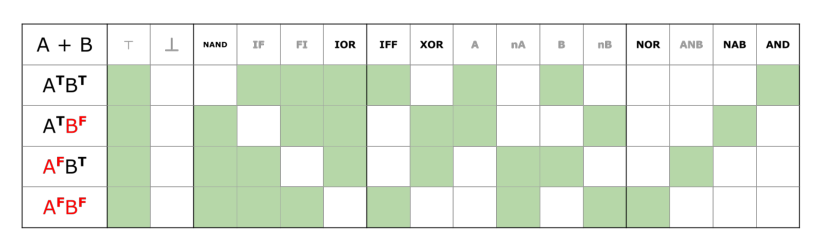
\includegraphics{figs/logicalConnectives-1} 

}

\caption{The truth table for the 16 binary logical connectives. The rows represent the set of situations where zero, one, or both propositions are true. The columns represent the 16 possible connectives and their truth conditions. Green cells represent true situations.}\label{fig:logicalConnectives}
\end{figure}
\begin{longtable}[]{@{}lll@{}}
\caption{\label{tab:connectiveInterpretaion} Annotation classes for
connective interpretation}\tabularnewline
\toprule
\begin{minipage}[b]{0.11\columnwidth}\raggedright\strut
Connective\strut
\end{minipage} & \begin{minipage}[b]{0.27\columnwidth}\raggedright\strut
Meaning\strut
\end{minipage} & \begin{minipage}[b]{0.54\columnwidth}\raggedright\strut
Examples\strut
\end{minipage}\tabularnewline
\midrule
\endfirsthead
\toprule
\begin{minipage}[b]{0.11\columnwidth}\raggedright\strut
Connective\strut
\end{minipage} & \begin{minipage}[b]{0.27\columnwidth}\raggedright\strut
Meaning\strut
\end{minipage} & \begin{minipage}[b]{0.54\columnwidth}\raggedright\strut
Examples\strut
\end{minipage}\tabularnewline
\midrule
\endhead
\begin{minipage}[t]{0.11\columnwidth}\raggedright\strut
AND\strut
\end{minipage} & \begin{minipage}[t]{0.27\columnwidth}\raggedright\strut
Both propositions are true\strut
\end{minipage} & \begin{minipage}[t]{0.54\columnwidth}\raggedright\strut
\emph{``I'm just gonna empty this and then I'll be out of the kitchen.''
-- ``I'll mix them together or I could mix it with carrot, too.''}\strut
\end{minipage}\tabularnewline
\begin{minipage}[t]{0.11\columnwidth}\raggedright\strut
IOR\strut
\end{minipage} & \begin{minipage}[t]{0.27\columnwidth}\raggedright\strut
One or both propositions are true\strut
\end{minipage} & \begin{minipage}[t]{0.54\columnwidth}\raggedright\strut
\emph{``You should use a spoon or a fork.'' -- ``Ask a grownup for some
juice or water or soy milk.''}\strut
\end{minipage}\tabularnewline
\begin{minipage}[t]{0.11\columnwidth}\raggedright\strut
XOR\strut
\end{minipage} & \begin{minipage}[t]{0.27\columnwidth}\raggedright\strut
Only one proposition is true\strut
\end{minipage} & \begin{minipage}[t]{0.54\columnwidth}\raggedright\strut
\emph{``Is that a hyena? or a leopard?'' -- ``We're gonna do things one
way or the other.''}\strut
\end{minipage}\tabularnewline
\begin{minipage}[t]{0.11\columnwidth}\raggedright\strut
NOR\strut
\end{minipage} & \begin{minipage}[t]{0.27\columnwidth}\raggedright\strut
Neither proposition is true\strut
\end{minipage} & \begin{minipage}[t]{0.54\columnwidth}\raggedright\strut
\emph{``I wouldn't say boo to one goose or three.'' -- ``She found she
lacked talent for hiding in trees, for chirping like crickets, or
humming like bees.''}\strut
\end{minipage}\tabularnewline
\begin{minipage}[t]{0.11\columnwidth}\raggedright\strut
IFF\strut
\end{minipage} & \begin{minipage}[t]{0.27\columnwidth}\raggedright\strut
Either both propositions are true or both are false\strut
\end{minipage} & \begin{minipage}[t]{0.54\columnwidth}\raggedright\strut
\emph{``Put them {[}crayons{]} up here and you can get down. -- Come
over here and I'll show you.''}\strut
\end{minipage}\tabularnewline
\begin{minipage}[t]{0.11\columnwidth}\raggedright\strut
NAB\strut
\end{minipage} & \begin{minipage}[t]{0.27\columnwidth}\raggedright\strut
The first proposition is false, the second is true.\strut
\end{minipage} & \begin{minipage}[t]{0.54\columnwidth}\raggedright\strut
\emph{``There's an Oatio here, or actually, there's a wheat
here.''}\strut
\end{minipage}\tabularnewline
\bottomrule
\end{longtable}
\paragraph{Intonation Type}\label{intonation-type}

For this category, annotators listened to the utterances and decided
whether the intonation contour on the coordination is flat, rise, or
rise-fall. Table @ref\label{tab:intonationTypes} shows the definitions and
examples for these intonation types. In order to judge the intonation of
the sentence accurately, annotators were asked to construct all three
intonation contours for the sentence and see which one is closer to the
actual intonation of the utterance. For example, to judge the sentence
``do you want orange juice\(\uparrow\) or apple juice\(\downarrow\)?'',
they reconstructed the sentence with the prototypical flat, rising, and
rise-fall intonations and checked to see which intonation is closer to
the actual one. It is important to note that while these three
intonation contours provide a good general classification, there is a
substantial degree of variation as well as a good number of subtypes
within each intonation type.
\begin{longtable}[]{@{}lll@{}}
\caption{\label{tab:intonationTypes} Definitions of the intonation types and
their examples.}\tabularnewline
\toprule
\begin{minipage}[b]{0.18\columnwidth}\raggedright\strut
Intonation Types\strut
\end{minipage} & \begin{minipage}[b]{0.30\columnwidth}\raggedright\strut
Definitions\strut
\end{minipage} & \begin{minipage}[b]{0.44\columnwidth}\raggedright\strut
Examples\strut
\end{minipage}\tabularnewline
\midrule
\endfirsthead
\toprule
\begin{minipage}[b]{0.18\columnwidth}\raggedright\strut
Intonation Types\strut
\end{minipage} & \begin{minipage}[b]{0.30\columnwidth}\raggedright\strut
Definitions\strut
\end{minipage} & \begin{minipage}[b]{0.44\columnwidth}\raggedright\strut
Examples\strut
\end{minipage}\tabularnewline
\midrule
\endhead
\begin{minipage}[t]{0.18\columnwidth}\raggedright\strut
Flat\strut
\end{minipage} & \begin{minipage}[t]{0.30\columnwidth}\raggedright\strut
Intonation does not show any substantial rise at the end of the
sentence.\strut
\end{minipage} & \begin{minipage}[t]{0.44\columnwidth}\raggedright\strut
\emph{``I don't hear any meows or bow-wow-wows.''}\strut
\end{minipage}\tabularnewline
\begin{minipage}[t]{0.18\columnwidth}\raggedright\strut
Rise\strut
\end{minipage} & \begin{minipage}[t]{0.30\columnwidth}\raggedright\strut
There is a substantial intonation rise on each disjunct or generally on
both.\strut
\end{minipage} & \begin{minipage}[t]{0.44\columnwidth}\raggedright\strut
\emph{``Do you want some seaweed? or some wheat germ?''}\strut
\end{minipage}\tabularnewline
\begin{minipage}[t]{0.18\columnwidth}\raggedright\strut
Rise-Fall\strut
\end{minipage} & \begin{minipage}[t]{0.30\columnwidth}\raggedright\strut
There is a substantial rise on the non-final disjunct(s), and a fall on
the final disjunct.\strut
\end{minipage} & \begin{minipage}[t]{0.44\columnwidth}\raggedright\strut
\emph{``Is that big Q or little q?'' -- ``(are) You patting them,
petting them, or slapping them?''}\strut
\end{minipage}\tabularnewline
\bottomrule
\end{longtable}
\paragraph{Utterance Type}\label{utterance-type}

Annotators decided whether an utterance is a declarative, an
interrogative, or an imperative. Table @ref (tab:utteranceTypes) provide
the definitions and examples for each utterance type. Occasionally, we
found examples with different utterance types for each coordinand. For
example, the mother would say ``put your backpack on and I'll be right
back'', where the first cooridnand is an imperative and the second a
declarative. Such examples were coded for both utterance types with a
dash in-between: imperative-declarative.
\begin{longtable}[]{@{}lll@{}}
\caption{\label{tab:utteranceTypes} Definitions of the utterance types and
their examples.}\tabularnewline
\toprule
\begin{minipage}[b]{0.16\columnwidth}\raggedright\strut
Utterance Types\strut
\end{minipage} & \begin{minipage}[b]{0.38\columnwidth}\raggedright\strut
Definitions\strut
\end{minipage} & \begin{minipage}[b]{0.38\columnwidth}\raggedright\strut
Examples\strut
\end{minipage}\tabularnewline
\midrule
\endfirsthead
\toprule
\begin{minipage}[b]{0.16\columnwidth}\raggedright\strut
Utterance Types\strut
\end{minipage} & \begin{minipage}[b]{0.38\columnwidth}\raggedright\strut
Definitions\strut
\end{minipage} & \begin{minipage}[b]{0.38\columnwidth}\raggedright\strut
Examples\strut
\end{minipage}\tabularnewline
\midrule
\endhead
\begin{minipage}[t]{0.16\columnwidth}\raggedright\strut
Declarative\strut
\end{minipage} & \begin{minipage}[t]{0.38\columnwidth}\raggedright\strut
Typically a statement with a subject-verb-object word order and a flat
intonation.\strut
\end{minipage} & \begin{minipage}[t]{0.38\columnwidth}\raggedright\strut
\emph{``It looks a little bit like a drum stick or a mallet.''}\strut
\end{minipage}\tabularnewline
\begin{minipage}[t]{0.16\columnwidth}\raggedright\strut
Interrogative\strut
\end{minipage} & \begin{minipage}[t]{0.38\columnwidth}\raggedright\strut
Typically a question with either subject-auxiliary inversion or a rising
terminal intonation.\strut
\end{minipage} & \begin{minipage}[t]{0.38\columnwidth}\raggedright\strut
\emph{``Is that a dog or a cat?''}\strut
\end{minipage}\tabularnewline
\begin{minipage}[t]{0.16\columnwidth}\raggedright\strut
Imperative\strut
\end{minipage} & \begin{minipage}[t]{0.38\columnwidth}\raggedright\strut
Typically a directive with an uninflected verb and no subject\strut
\end{minipage} & \begin{minipage}[t]{0.38\columnwidth}\raggedright\strut
\emph{``Have a little more French toast or have some of your
juice.''}\strut
\end{minipage}\tabularnewline
\bottomrule
\end{longtable}
\paragraph{Syntactic Level}\label{syntactic-level}

For this annotation category, annotators decided whether the
coordination is at the clausal level or at the sub-clausal level.
Clausal level was defined as sentences, clauses, verb phrases, and
verbs. Coordination of other categories was coded as sub-clausal. This
annotation category was introduced to check the hypothesis that the
syntactic category of the coordinands may influence the interpretation
of a coordination. The intuition was that a sentence such as ``He drank
tea or coffee'' is less likely to be interpreted as exclusive than ``He
drank tea or he drink coffee.'' The clausal vs.~sub-clausal distinction
was inspired by the fact that in many languages, coordinators that
connect sentences and verb phrases are different lexical items than
those that connect nominal, adjectival, or prepositional phrases (see
Haspelmath, 2007).
\begin{longtable}[]{@{}lll@{}}
\caption{\label{tab:syntacticLevel} Definitions of the syntactic levels and
their examples.}\tabularnewline
\toprule
\begin{minipage}[b]{0.17\columnwidth}\raggedright\strut
Syntactic Level\strut
\end{minipage} & \begin{minipage}[b]{0.37\columnwidth}\raggedright\strut
Definitions\strut
\end{minipage} & \begin{minipage}[b]{0.37\columnwidth}\raggedright\strut
Examples\strut
\end{minipage}\tabularnewline
\midrule
\endfirsthead
\toprule
\begin{minipage}[b]{0.17\columnwidth}\raggedright\strut
Syntactic Level\strut
\end{minipage} & \begin{minipage}[b]{0.37\columnwidth}\raggedright\strut
Definitions\strut
\end{minipage} & \begin{minipage}[b]{0.37\columnwidth}\raggedright\strut
Examples\strut
\end{minipage}\tabularnewline
\midrule
\endhead
\begin{minipage}[t]{0.17\columnwidth}\raggedright\strut
Clausal\strut
\end{minipage} & \begin{minipage}[t]{0.37\columnwidth}\raggedright\strut
The coordinands are sentences, clauses, verb phrases, or verbs.\strut
\end{minipage} & \begin{minipage}[t]{0.37\columnwidth}\raggedright\strut
\emph{``Does he lose his tail sometimes and Pooh helps him and puts it
back on?''}\strut
\end{minipage}\tabularnewline
\begin{minipage}[t]{0.17\columnwidth}\raggedright\strut
Sub-clausal\strut
\end{minipage} & \begin{minipage}[t]{0.37\columnwidth}\raggedright\strut
The coordinands are nouns, adjectives, noun phrases, determiner phrases,
or prepositional phrases.\strut
\end{minipage} & \begin{minipage}[t]{0.37\columnwidth}\raggedright\strut
\emph{``Hollies can be bushes or trees.''}\strut
\end{minipage}\tabularnewline
\bottomrule
\end{longtable}
\paragraph{Conceptual Consistency}\label{conceptual-consistency}

Propositions that are connected by words such as \emph{and} and
\emph{or} often stand in complex conceptual relations with each other.
For conceptual consistency, annotators decided whether the propositions
that make up the coordination can be true at the same time or not. If
the two propositions could be true at the same time they were marked as
consistent. If the two propositions could not be true at the same time
and resulted in a contradiction, they were marked as inconsistent. Our
annotators used the following diagnostic to decide the consistency of
the disjuncts: Two disjuncts were marked as inconsistent if replacing
the word \emph{or} with \emph{and} produced a contradiction. For
example, changing ``the ball is in my room \emph{or} your room'' to
``the ball is in my room \emph{and} your room'' produces a contradiction
because a ball cannot be in two rooms at the same time.
\begin{longtable}[]{@{}lll@{}}
\caption{\label{tab:consistencyType} Definitions of the intonation types and
their examples.}\tabularnewline
\toprule
\begin{minipage}[b]{0.20\columnwidth}\raggedright\strut
Consistency\strut
\end{minipage} & \begin{minipage}[b]{0.16\columnwidth}\raggedright\strut
Definitions\strut
\end{minipage} & \begin{minipage}[b]{0.42\columnwidth}\raggedright\strut
Examples\strut
\end{minipage}\tabularnewline
\midrule
\endfirsthead
\toprule
\begin{minipage}[b]{0.20\columnwidth}\raggedright\strut
Consistency\strut
\end{minipage} & \begin{minipage}[b]{0.16\columnwidth}\raggedright\strut
Definitions\strut
\end{minipage} & \begin{minipage}[b]{0.42\columnwidth}\raggedright\strut
Examples\strut
\end{minipage}\tabularnewline
\midrule
\endhead
\begin{minipage}[t]{0.20\columnwidth}\raggedright\strut
Consistent\strut
\end{minipage} & \begin{minipage}[t]{0.16\columnwidth}\raggedright\strut
The coordinands can be true at the same time.\strut
\end{minipage} & \begin{minipage}[t]{0.42\columnwidth}\raggedright\strut
\emph{``We could spell some things with a pen or draw some
pictures.''}\strut
\end{minipage}\tabularnewline
\begin{minipage}[t]{0.20\columnwidth}\raggedright\strut
Inconsistent\strut
\end{minipage} & \begin{minipage}[t]{0.16\columnwidth}\raggedright\strut
The coordinands cannot be true at the same time.\strut
\end{minipage} & \begin{minipage}[t]{0.42\columnwidth}\raggedright\strut
\emph{``Do you want warm or cold tomato sauce?''}\strut
\end{minipage}\tabularnewline
\bottomrule
\end{longtable}
First, it is important to note here that this criterion is quite strict.
In many cases, the possibility of both propositions being true is ruled
out based on prior knowledge and expectations of the situation. For
example, when asking people whether they would like tea or coffee, it is
often assumed and expected that people choose one or the other. However,
wanting to drink both tea and coffee is not conceptually inconsistent.
It is just very unlikely. Our annotations of consistency are very
conservative in that they still consider such unlikely cases as
consistent.

Second, there are much more complex relations between coordinated
propositions that we have not coded for. For example, coordinated
propositions sometimes stand in a causal relation (e.g.~the cup fell and
broke) or sometimes in a temporal relation (e.g.~she brushed her teeth
and went to bed), among many more. It is quite feasible to assume that
the rich conceptual structure of these propositions help children learn
the meaning and use of connectives such as \emph{and}, \emph{or},
\emph{if}, \emph{therefore}, etc. It is possible to develop a more
detailed investigation on the relation between propositions and how that
affects the acquisition of connective meaning generally. However, in
this study we mainly focus on conceptual consistency of the coordinated
propositions and how that affects the acquisition of \emph{and} and
\emph{or}.

It is also important to note that if the coordinands are inconsistent,
this does not necessarily means that the connective interpreation must
be exclusive. For example, in a sentence like ``you could stay here or
go out'', the alternatives ``staying here'' and ``going out'' are
inconsistent. Yet, the overall interpretation of the connective could be
conjunctive: you could stay here AND you could go out. The statement
communicates that both possibilities hold. This pattern of interaction
between possibility modals like \emph{can} and disjunction words like
\emph{or} are often discussed under the lable ``free-choice inferences''
in the semantics and pragmatics literature (Kamp, 1973; Von Wright,
1968). Another example is unconditionals such as ``Ready or not, here I
come!''. The coordinands are contradictions: one is the negation of the
other. However, the overall interpretation of the sentences is that in
both cases, the speaker is going to come.

\paragraph{Communicative Functions}\label{communicative-functions}

This study constructed a set of categories that captured particular
usages or communiative functions of the words \emph{or} and \emph{and}.
These communicative functions were created using the first 100
annotation examples and then they were used for the classification of
the rest of the examples. Table \ref{tab:speechActs} shows the
definitions and examples of the 10 communicative functions used in this
study. The table contains some functions that are general and some that
are specific to coordination. For example, directives are a general
class while conditionals are more specific to coordinated constructions.
It is also important to note that the list is not an unstructured one;
we see some communicative functions as subtypes of others. For example,
``identifications'' and ``unconditionals'' are sybtypes of
``descriptions'' while ``conditionals'' are a subtype of directives.
Furthuremore, ``repairs'' seem parallel to other categories in that any
speech at can be repaired. We do not fully explore the details of these
functions in this study but such details matter for a general theory of
acquisition that makes use of the speaker's communicative intentions as
early coarse-grained communicative cues for the acquisition of
fine-grained meaning such as function words.
\begin{longtable}[]{@{}lll@{}}
\caption{\label{tab:speechActs} Definitions of the communicative functions
and their examples.}\tabularnewline
\toprule
\begin{minipage}[b]{0.14\columnwidth}\raggedright\strut
Answer Type\strut
\end{minipage} & \begin{minipage}[b]{0.44\columnwidth}\raggedright\strut
Definitions\strut
\end{minipage} & \begin{minipage}[b]{0.33\columnwidth}\raggedright\strut
Examples\strut
\end{minipage}\tabularnewline
\midrule
\endfirsthead
\toprule
\begin{minipage}[b]{0.14\columnwidth}\raggedright\strut
Answer Type\strut
\end{minipage} & \begin{minipage}[b]{0.44\columnwidth}\raggedright\strut
Definitions\strut
\end{minipage} & \begin{minipage}[b]{0.33\columnwidth}\raggedright\strut
Examples\strut
\end{minipage}\tabularnewline
\midrule
\endhead
\begin{minipage}[t]{0.14\columnwidth}\raggedright\strut
Descriptions\strut
\end{minipage} & \begin{minipage}[t]{0.44\columnwidth}\raggedright\strut
describing what the world is like or asking about it. The primary goal
is to inform the addressee about how things are.\strut
\end{minipage} & \begin{minipage}[t]{0.33\columnwidth}\raggedright\strut
``\emph{It's not in the ditch or the drain pipe.}''\strut
\end{minipage}\tabularnewline
\begin{minipage}[t]{0.14\columnwidth}\raggedright\strut
Identifications\strut
\end{minipage} & \begin{minipage}[t]{0.44\columnwidth}\raggedright\strut
Identifying the category membership or an attribute of an object.
Speaker has uncertainty. A subtype of ``Description''.\strut
\end{minipage} & \begin{minipage}[t]{0.33\columnwidth}\raggedright\strut
``\emph{Is that a ball or a balloon honey?}''\strut
\end{minipage}\tabularnewline
\begin{minipage}[t]{0.14\columnwidth}\raggedright\strut
Definitions and Examples\strut
\end{minipage} & \begin{minipage}[t]{0.44\columnwidth}\raggedright\strut
Providing labels for a category or examples for it. Speaker has no
uncertainty. Subtype of Description.\strut
\end{minipage} & \begin{minipage}[t]{0.33\columnwidth}\raggedright\strut
\emph{``this is a cup or a mug.'' -- ``berries like blueberry or
raspberry''}\strut
\end{minipage}\tabularnewline
\begin{minipage}[t]{0.14\columnwidth}\raggedright\strut
Preferences\strut
\end{minipage} & \begin{minipage}[t]{0.44\columnwidth}\raggedright\strut
Asking what the addressee wants or would like or stating what the
speaker wants or would like\strut
\end{minipage} & \begin{minipage}[t]{0.33\columnwidth}\raggedright\strut
\emph{``do you wanna play pizza or read the book?''}\strut
\end{minipage}\tabularnewline
\begin{minipage}[t]{0.14\columnwidth}\raggedright\strut
Options\strut
\end{minipage} & \begin{minipage}[t]{0.44\columnwidth}\raggedright\strut
Either asking or listing what one can or is allowed to do. Giving
permission, asking for permission, or describing the possibilities.
Often the modal ``can'' is either present or can be inserted.\strut
\end{minipage} & \begin{minipage}[t]{0.33\columnwidth}\raggedright\strut
\emph{``you could have wheat or rice.''}\strut
\end{minipage}\tabularnewline
\begin{minipage}[t]{0.14\columnwidth}\raggedright\strut
Directives\strut
\end{minipage} & \begin{minipage}[t]{0.44\columnwidth}\raggedright\strut
Directing the addressee to act or not act in a particular way. Common
patterns include ``let's do \ldots{}'', ``Why don't you do \ldots{}'',
or prohibitions such as ``Don't \ldots{}''. The difference with
``options'' is that the speaker expects the directive to be carried out
by the addressee. There is no such expectation for ``options''.\strut
\end{minipage} & \begin{minipage}[t]{0.33\columnwidth}\raggedright\strut
\emph{``let's go back and play with your ball or we'll read your
book.''}\strut
\end{minipage}\tabularnewline
\begin{minipage}[t]{0.14\columnwidth}\raggedright\strut
Clarifications\strut
\end{minipage} & \begin{minipage}[t]{0.44\columnwidth}\raggedright\strut
Something is said or done as a communicative act but the speaker has
uncertainty with respect to the form or the content.\strut
\end{minipage} & \begin{minipage}[t]{0.33\columnwidth}\raggedright\strut
\emph{``you mean boba or bubble?''}\strut
\end{minipage}\tabularnewline
\begin{minipage}[t]{0.14\columnwidth}\raggedright\strut
Repairs\strut
\end{minipage} & \begin{minipage}[t]{0.44\columnwidth}\raggedright\strut
Speaker correcting herself on something she said (self repair) or
correcting the addressee (other repair). The second disjunct is what
holds and is intended by the speaker. The speaker does not have
uncertainty with respect to what actually holds.\strut
\end{minipage} & \begin{minipage}[t]{0.33\columnwidth}\raggedright\strut
\emph{``There's an Oatio here, or actually, there's a wheat
here.''}\strut
\end{minipage}\tabularnewline
\begin{minipage}[t]{0.14\columnwidth}\raggedright\strut
Conditionals\strut
\end{minipage} & \begin{minipage}[t]{0.44\columnwidth}\raggedright\strut
Explaining in the second coordinand, what would follow if the first
coordinand is (or is not) followed. Subtype of Directive.\strut
\end{minipage} & \begin{minipage}[t]{0.33\columnwidth}\raggedright\strut
\emph{``put that out of your mouth, or I'm gonna put it away.''} --
\emph{``Come over here and I'll show you.''}\strut
\end{minipage}\tabularnewline
\begin{minipage}[t]{0.14\columnwidth}\raggedright\strut
Unconditionals\strut
\end{minipage} & \begin{minipage}[t]{0.44\columnwidth}\raggedright\strut
Denying the dependence of something on a set of conditions. Typical
format: ``whether X or Y, Z''. Subtype of Descriptions.\strut
\end{minipage} & \begin{minipage}[t]{0.33\columnwidth}\raggedright\strut
\emph{``Ready or not, here I come!''} (playing hide and seek)\strut
\end{minipage}\tabularnewline
\bottomrule
\end{longtable}
\paragraph{Answer Type}\label{answer-type}

Whenever a parent's utterance was a polar question, the annotators coded
the utterance for the type of response it received from the children.
Table \ref{tab:answerTypes} shows the answer types in this study and
their definitions and examples. Utterances that were not polar questions
were simply coded as NA for this category. If children responded to
polar questions with ``yes'' or ``no'', the category was YN and if they
repeated with one of the coordinands the category was AB. If children
said yes/no and followed it with one of the coordinands, the answer type
was determined as YN (yes/no). For example, if a child was asked ``Do
you want orange juice or apple juice?'' and the child responded with
``yes, apple juice'', our annotators coded the response as YN. The
reason is that in almost all cases, if a simple yes/no response is
felicitous, then it can also be optionally followed with mentioning a
disjunct. However, if yes/no is not a felicitous response, then
mentioning one of the alternatives is the only appropriate answer. For
example, if someone asks ``Do you want to stay here or go out?'' a
response such as ``yes, go out'' is infelicitous and a better response
is to simply say ``go out''. Therefore, we count responses with both
yes/no and mentioning an alternative as a yes/no response.
\begin{longtable}[]{@{}lll@{}}
\caption{\label{tab:answerTypes} Definitions of answer types and their
examples.}\tabularnewline
\toprule
\begin{minipage}[b]{0.11\columnwidth}\raggedright\strut
Answer Type\strut
\end{minipage} & \begin{minipage}[b]{0.32\columnwidth}\raggedright\strut
Definitions\strut
\end{minipage} & \begin{minipage}[b]{0.38\columnwidth}\raggedright\strut
Examples\strut
\end{minipage}\tabularnewline
\midrule
\endfirsthead
\toprule
\begin{minipage}[b]{0.11\columnwidth}\raggedright\strut
Answer Type\strut
\end{minipage} & \begin{minipage}[b]{0.32\columnwidth}\raggedright\strut
Definitions\strut
\end{minipage} & \begin{minipage}[b]{0.38\columnwidth}\raggedright\strut
Examples\strut
\end{minipage}\tabularnewline
\midrule
\endhead
\begin{minipage}[t]{0.11\columnwidth}\raggedright\strut
No Answer\strut
\end{minipage} & \begin{minipage}[t]{0.32\columnwidth}\raggedright\strut
The child provides no answer to the question.\strut
\end{minipage} & \begin{minipage}[t]{0.38\columnwidth}\raggedright\strut
Mother: \emph{``Would you like to eat some applesauce or some
carrots?\emph{" Child: }''Guess what Max!}``\strut
\end{minipage}\tabularnewline
\begin{minipage}[t]{0.11\columnwidth}\raggedright\strut
YN\strut
\end{minipage} & \begin{minipage}[t]{0.32\columnwidth}\raggedright\strut
The child responds with yes or no\strut
\end{minipage} & \begin{minipage}[t]{0.38\columnwidth}\raggedright\strut
Father: \emph{``Can I finish eating one or two more bites of my
cereal?''} Child: \emph{``No.''}\strut
\end{minipage}\tabularnewline
\begin{minipage}[t]{0.11\columnwidth}\raggedright\strut
AB\strut
\end{minipage} & \begin{minipage}[t]{0.32\columnwidth}\raggedright\strut
The child responds with one of the disjuncts (alternatives)\strut
\end{minipage} & \begin{minipage}[t]{0.38\columnwidth}\raggedright\strut
Mother: \emph{``Is she a baby elephant or is she a toddler elephant?''}
Child: \emph{``It's a baby. She has a tail.''}\strut
\end{minipage}\tabularnewline
\bottomrule
\end{longtable}
\subsubsection{Inter-annotator
Reliability}\label{inter-annotator-reliability}

To train annotators and confirm their reliaiblity for disjunction
examples, two annotators coded the same 240 instances of disjunction.
The inter-annotator reliability was calculated over 8 iterations of 30
examples each. After each iteration, annotators met to discuss
disagreements and resolve them. They also decided whether the category
definitions or annotation criteria needed to be made more precise.
Training was completed after three consecutive iterations showed
substantial agreement between the annotators (Cohen's \(\kappa > 0.7\))
for all categories. Figure \ref{fig:oReliabilityPlot} shows the
precentage agreement and the kappa values for each annotation category
over the 8 iterations.
\begin{figure}[tb]

{\centering 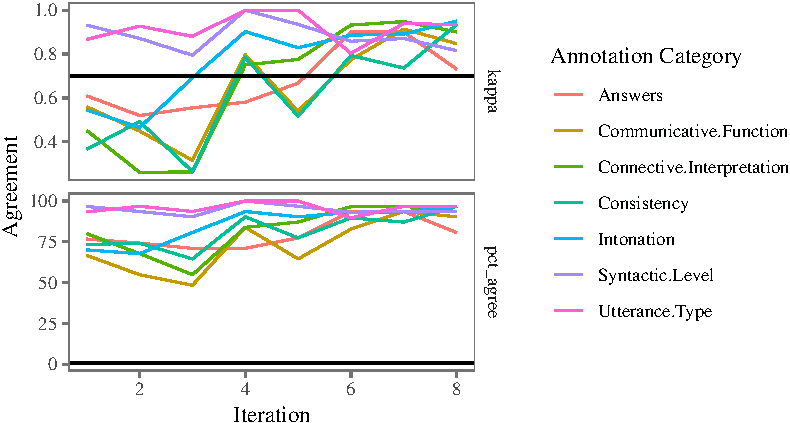
\includegraphics{figs/oReliabilityPlot-1} 

}

\caption{Inter-annotator agreement for disjunction examples.}\label{fig:oReliabilityPlot}
\end{figure}
Agreement in three catgories showed substantial improvement after better
and more precise deifinitions and annotation criteria were developed:
connective interpretation, intonation, and communicative function.
First, connective interpretation showed major improvements after
annotators developed more precise criteria for selecting the
propositions under discussion and separately wrote down the two
propositions connected by the connective word. For example, if the
original utterance was ``do you want milk or juice?'', the annotators
wrote ``you want milk, you want juice'' as the two propositions under
discussion. This exercise clarified the exact propositions under
discussion and sharpened annotator intuitions with respect to the
connnective interpretation that is communicated by the utterance.
Second, annotators improved agreement on intonation by reconstructing an
utterance's intonation for all three intonation categories. For example,
the annotator would examine the same sentence ``do you want coffee or
tea?'' with a rise-fall, a rise, and a flat intonation. Then the
annotator would listen to the actual utterance and see which one better
resembles the actual utterance. This method helped annotators judge the
intonation of an utterance more accurately. Finally, agreement on
communicative functions improved as the definitions were made more and
more precise. For example, the definition of ``directives'' in Table
\ref{tab:speechActs} explicitly mentions the difference between
``directives'' and ``options''. Clarifying the definitions of
communicative functions helped improve annotator agreement.

Inter-annotator reliability for conjunction was calculated similar to
disjunction examples. Two different annotators coded 300 utterances of
\emph{and}. Inter-annotator reliability was calculated over 10
iterations of 30 examples. Figure \ref{fig:andReliabilityPlot} shows the
precentage agreement between the annotators as well as the kappa values
for each iteration. Despite high percentage agreement between
annotators, the kappa values did not pass the set threshold of 0.7 in
three consecuitive iterations. This paradoxical result is mainly due to
a property of kappa. An imbalance in the prevalence of annotation
categories can drastically lower the value of kappa. When one category
is extremely common with high agreement while other categories are rare,
kappa will be low (Cicchetti \& Feinstein, 1990; Feinstein \& Cicchetti,
1990). In almost all annotated categories for conjunction, there was one
class that was extremely prevalent. In such cases, it is much more
informative to look at the class specific agreement for the prevalent
category than the overall agreement measured by Kappa (Cicchetti \&
Feinstein, 1990; Feinstein \& Cicchetti, 1990).
\begin{figure}[tb]

{\centering 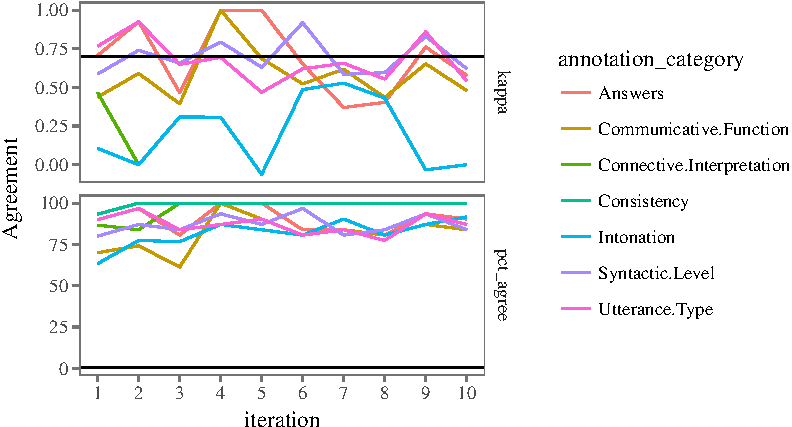
\includegraphics{figs/andReliabilityPlot-1} 

}

\caption{Inter-annotator agreement for disjunction examples.}\label{fig:andReliabilityPlot}
\end{figure}
Table \ref{tab:andAgreeStats} lists the dominant classes as well as
their prevalence, the values of class specific agreement index, and
category agreement index (Kappa). Class specific agreement index is
defined as \(2n_{ii}/n_{i.}+n_{.i}\), where \(i\) represents the class's
row/column number in the category's confusion matrix, \(n\) the number
of annotations in a cell, and the dot ranges over all the row/column
numbers (Fleiss, Levin, \& Paik, 2013, p. 600; Ubersax, 2009). The class
specific agreement indeces are very high for all the most prevalent
classes showing that the annotators had very high agreement on these
class, even though the general agreement index (Kappa) was often low.
The most extreme case is the category ``consistency'' where almost all
instances were annotated as ``consistent'' with perfect class specific
agreement but low overall Kappa. In the case of utterance type and
syntactic level where the distribution of instances across classes was
more even, the general index of agreement Kappa is also high. In
general, examples of conjunction showed little variablility across
annotation categories and mostly fell into one class within each
category. Annotators had very high agreement for these dominant classes.
\begin{table}

\caption{\label{tab:andAgreeStats}Most prevalent annotation class in each annotation category with the values of class agreement indeces and category agreement indeces (Kappa).}
\centering
\begin{tabular}[t]{l|l|r|r|r}
\hline
Annotation Category & Class & Prevalence & Class Agreement Index & Kappa\\
\hline
intonation & flat & 0.86 & 0.89 & 0.24\\
\hline
interpretation & AND & 0.96 & 0.98 & 0.39\\
\hline
answer & NA & 0.84 & 0.94 & 0.67\\
\hline
utterance\_type & declarative & 0.76 & 0.94 & 0.70\\
\hline
communicative\_function & description & 0.77 & 0.90 & 0.59\\
\hline
syntactic\_level & clausal & 0.67 & 0.91 & 0.70\\
\hline
consistency & consistent & 0.99 & 1.00 & 0.50\\
\hline
\end{tabular}
\end{table}
\subsection{Results}\label{results-3}

First, I show the results for the study's dependent measure\footnote{All
  the confidence intervals shown in the plots for this section are
  simultaneous multinomial confidence intervals computed using the Sison
  \& Glaz (1995)'s method}. Figure (\ref{fig:interpretationPlot}) shows
the distribution of the connective interpretations in the study. The
most common interpretation was the conjunctive interpretation AND (0.49)
followed by the exclusive XOR (0.35). Figure (\ref{fig:connectivePlot})
shows the distribution of connective interpretations by the connective
words \emph{and} and \emph{or}. For \emph{and}, the most frequent
interpretation (in fact almost the only interpretation), is conjunction
AND. For \emph{or}, the most frequent interpretation is exclusive
disjunction XOR. These results replicate the findings of Morris (2008).
\begin{figure}[tb]

{\centering 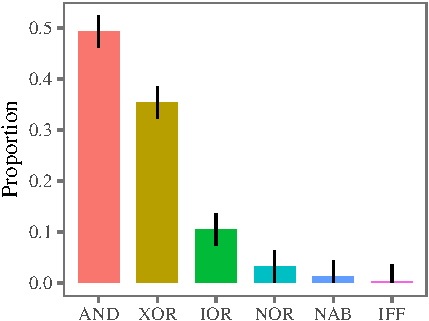
\includegraphics{figs/interpretationPlot-1} 

}

\caption{The proportion of different interpretations of the connectives and/or in child-directed speech}\label{fig:interpretationPlot}
\end{figure}
\begin{figure}[tb]

{\centering 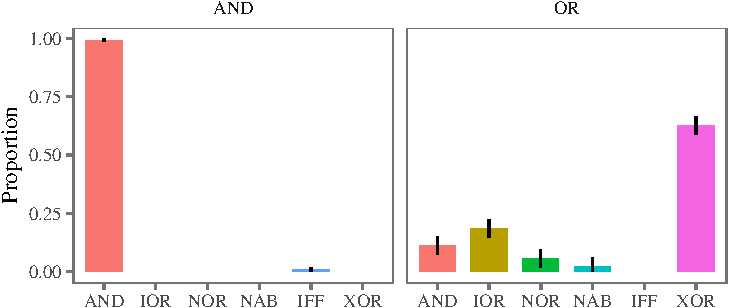
\includegraphics{figs/connectivePlot-1} 

}

\caption{Interpretations of and/or in child-directed speech}\label{fig:connectivePlot}
\end{figure}
Based on these results, Morris argued that given the high frequency of
conjunction and exclusive disjunction in the input, children should map
the meanings of \emph{and} and \emph{or} as conjunction and exclusive
disjunction, at least initially, between the ages of 2 and 5. Children
learn the inclusive interpretation of disjunction later as they
encounter more inclusive (logical) uses of \emph{or}. However,
comprehension tasks show that children between 3 and 5 tend to interpret
\emph{or} as inclusive disjunction rather than exclusive disjunction in
a variety of declarative sentences (Chierchia et al., 2001; Gualmini et
al., 2000a, 2000b, among others; Notley et al., 2012). How can children
learn the inclusive semantics of \emph{or} if they rarely hear it? The
remainder of this section explore the role of cues in child directed
speech that could help children successfully interpret a disjunction as
inclusive or exclusive.
\begin{figure}[tb]

{\centering 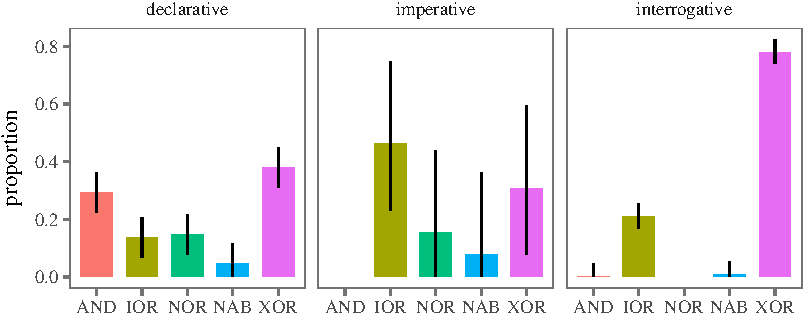
\includegraphics{figs/utterancetypePlot-1} 

}

\caption{Connective interpretations in different sentence types.}\label{fig:utterancetypePlot}
\end{figure}
I will first look at the effect of utterance type on the interpretation
of \emph{or}. Figure \ref{fig:utterancetypePlot} shows the distribution
of connective interpretations in declarative, interrogative, and
imperative sentences. Interrogatives are more likely to be interpreted
as exclusive disjunction XOR, imperatives are more likely to be
interpreted as inclusive or exclusive, and declaratives are most likely
exclusive XOR or conjunctive AND. It is important to note here that the
inclusive interpretations of imperatives are largely due to invitations
to action such as ``Have some food or drink!''. Such invitational
imperatives seem to convey inclusivity IOR systematically. They are
often used to give addressee full permission with respect to both
alternatives and it seems quite odd to use them to imply exclusivity
(``have some food or drink but not both!''), and they do not seem to be
conjunctive either (``have some food and have some drink''). They rather
imply that the addressee is invited to have food, drink, or both.
\begin{figure}[tb]

{\centering 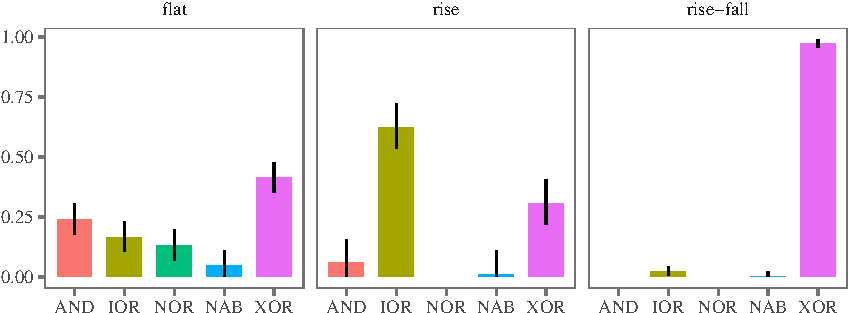
\includegraphics{figs/intonationPlot-1} 

}

\caption{The distribution of connective interpretations in flat, rising, and rise-fall intonation contours.}\label{fig:intonationPlot}
\end{figure}
Figure (\ref{fig:intonationPlot}) shows the proportions of different
connective interpretations in the three intonation contours: flat, rise,
and rise-fall. A disjunction with a rise-fall intonation is most likely
interpreted as exclusive XOR. A disjunction is more likely to be
interpreted as inclusive IOR if the intonation is rising. And a
disjunction with a flat intonation may be interpreted as exclusive XOR,
conjunctive AND, or inclusive IOR. These results are consistent with
Pruitt \& Roelofsen (2013)'s experimental findings that a rise-fall
intonation contour on a disjunction results in an exclusive
interpretation. Since rise-fall and rising intonation contours are
almost always on interrogatives, Figures \ref{fig:utterancetypePlot} and
\ref{fig:intonationPlot}, suggest that the rise-fall and rising
intonation types distinguish exclusive and inclusive interpretations of
disjunction in interrogatives. Furthermore, given a flat intonation
type, an imperative may be more likely to be inclusive.
\begin{figure}[tb]

{\centering 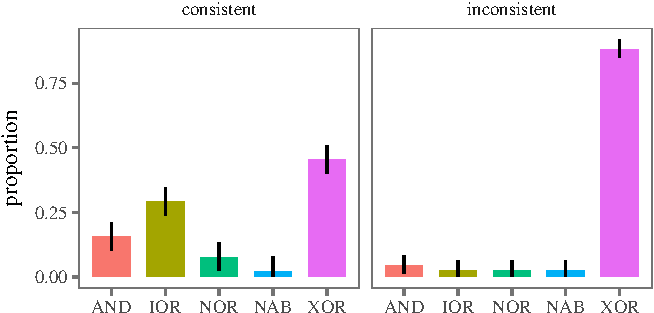
\includegraphics{figs/consistencyPlot-1} 

}

\caption{Connective interpretations in disjunctions with consistent and inconsistent disjuncts.}\label{fig:consistencyPlot}
\end{figure}
Figure \ref{fig:consistencyPlot} shows the proportions of connective
interpretations in disjunctions with consistent vs.~inconsistent
disjuncts. When the disjuncts were consistent, the interpretation could
be exclusive XOR, inclusive IOR, or conjunctive AND. When the disjuncts
were inconsistent, however, a disjunction almost always received an
exclusive XOR interpretation. These results suggest that the exclusive
interpretation of a disjunction often stems from the inconsistent or
contradictory nature of the disjuncts themselves and not necessarily the
connective word \emph{or}. It should be noted here that in all
\emph{and}-examples, the disjuncts were consistent. This is not
surprising given that inconsistent meanings with \emph{and} result in a
contradiction. The only exception to this was one example where the
mother was mentioning two words as antonyms: ``short and tall''. This
example is quite different from the normal utterances given that it is
meta-linguistic and list words rather than asserting the content of the
words.
\begin{figure}[tb]

{\centering 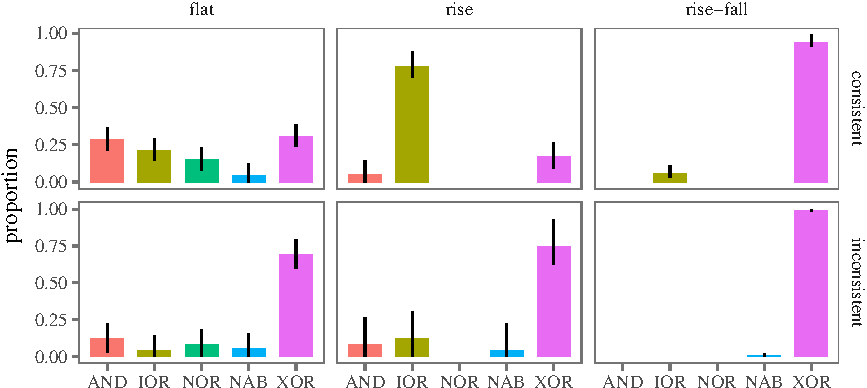
\includegraphics{figs/consistencyByintonationPlot-1} 

}

\caption{Interpretations of and/or in the three intonation contours flat, rising, and rise-fall.}\label{fig:consistencyByintonationPlot}
\end{figure}
In Figure \ref{fig:consistencyByintonationPlot}, I break down connective
interpretations by both intonation and consistency. The results show
that disjunctions are interpreted as exclusive XOR when they carry
either inconsistent disjuncts or a rise-fall intonation. If the
disjunction has consistent disjuncts and carries a rising intonation, it
is most likely interpreted as inclusive IOR. Disjunctions with
consistent disjuncts and a flat intonation contour could have
conjunctive AND, inclusive IOR, or exclusive XOR interpretations.
\begin{figure}[tb]

{\centering 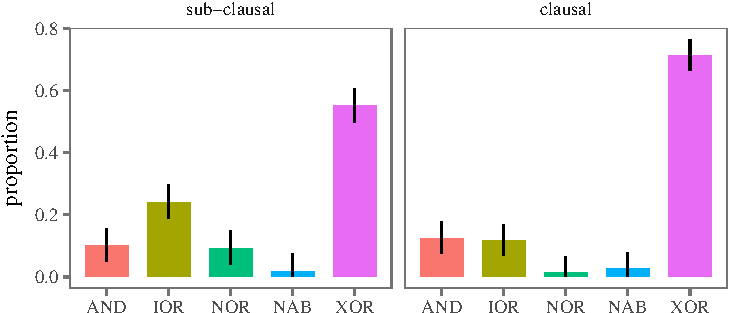
\includegraphics{figs/syntaxPlot-1} 

}

\caption{Connective interpretations in clausal and sub-clausal disjunctions.}\label{fig:syntaxPlot}
\end{figure}
Figure \ref{fig:syntaxPlot} shows connective interpretations by the
syntactic level of the disjunction. As a reminder, we annotated
disjunctions with clausal and verbal disjuncts as ``clausal'' and those
with other syntactic categories as sub-clausal. The goal was to assess
the role of syntax in the interpretation of disjunction. The results
suggest a small effect of clausal level disjuncts. Disjunctions are more
likely to be interpreted as exclusive when their disjuncts are clauses
or verbs rather than nominals, adjectives, or prepositions (all
sub-clausal units).
\begin{figure}[tb]

{\centering 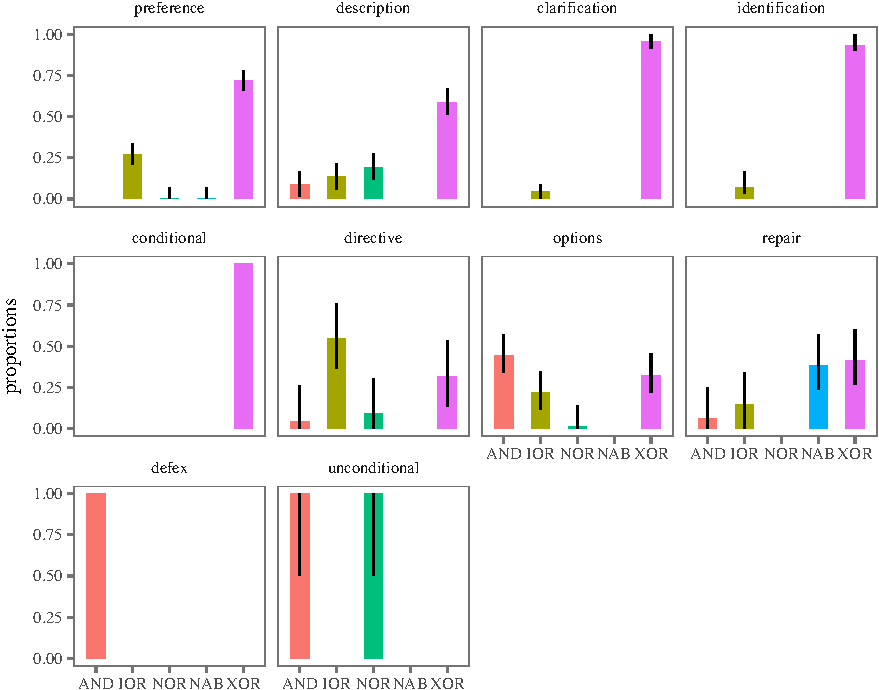
\includegraphics{figs/speechActPlot-1} 

}

\caption{Connective interpretations in different communicative functions.}\label{fig:speechActPlot}
\end{figure}
For the last independent variable in our study, I take a look at how
disjunction interpretations are affected by the communicative function
of the utterance they appear in. Figure \ref{fig:speechActPlot} shows
the proportions of connective interpretations in the 10 different
communicative functions of this study. The results show that certain
functions increase the likelihood of some connective interpretations. An
exclusive XOR interpretation of \emph{or} is common in acts of
clarification, identification, stating/asking preferences,
stating/asking about a description, or making a conditional statements.
These results are consistent with expectations on the communicative
intentions of that these utterances carry. In clarifications, the
speaker needs to know which of two alternatives the other party meant.
Similarly in identifications, speaker needs to know which category does
a referent belongs to. In preferences, parents seek to know which of two
alternatives the child wants. Even though descriptions could be either
inclusive or exclusive, in the current sample most descriptions were
questions about the state of affairs and required the child to provide
one of the alternatives as the answer. In conditionals such as ``come
here or you are grounded'', the point of the threat is that only one
disjunct can be true: either ``you come and you are not grounded'' or
``you don't come and you are grounded''. This is similar to an exclusive
interpretation of \emph{or}.

Repairs often received an exclusive XOR or a second disjunct true NAB
interpretation. This is expected given that in repairs the speaker
intends to say that the first disjunct is incorrect or inaccurate.
Unconditionals and definitions/examples always had a conjunctive AND
interpretation. Again, this is to be expected. In such cases the speaker
intends to communicate that all options apply. If the mother says that
cats are animals like lions or tigers, she intends to say that both
lions and tigers are cats and not one or the other. Interestingly, in
some cases (not all), \emph{or} is replaceable by and: cats are animals
like lions and tigers. In unconditionals, the speaker communicates that
in both alternatives, a certain proposition holds. For example, if the
mother says ``ready or not, here I come!'', she communicates that ``I
come'' is true in both ``you are ready'' and ``you are not ready''.

Options were often interpreted either as conjunctive AND or inclusive
IOR. The category options contained examples of free-choice inferences
such as ``you could drink orange juice or apple juice''. This study
found free-choice examples much more common than the current literature
on the acquisition of disjunction suggests. Finally, directives received
either an IOR or XOR interpretation. It is important to note here that
the most common communcative function in the data were preferences and
descriptions. Other communicative functions such as unconditionals or
options were fairly rare. Despite their infrequent appearance, these
constructions must be learned by children at some point, since almost
all adults know how to interpret them. It is clear from the
investigation here that any learning account for function word
meaning/interpretation also needs to account for how such infrequent
constructions are learned.

Finally, I take a look at how children responded to the questions
containing \emph{and} and \emph{or}. As a reminder, we annotated every
polar question such as ``do you want cereal or toast?'' for the type of
answer children provided. An answer such as ``yes/no'' is annotated as
YN and an answer with alternatives such as ``cereal/toast'' is annotated
as ``AB''. Figure (\ref{fig:answerPlot}) shows the monthly proportions
of these answer types between 1 and 3 years of age. Initially, children
provide noy answer to polar questions, but by the age 3, the majority of
such questions receive a yes/no (YN) or alternative (AB) answer.
\begin{figure}[tb]

{\centering 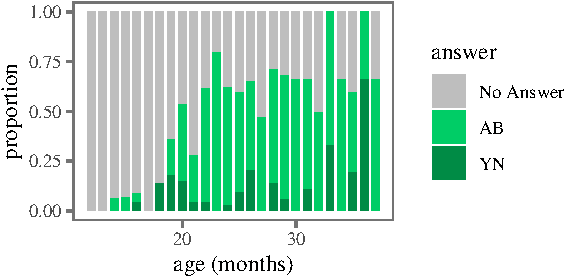
\includegraphics{figs/answerPlot-1} 

}

\caption{The proportions of children's answer types to polar questions containing the connectives and/or at different ages (in months).}\label{fig:answerPlot}
\end{figure}
These two answer types are not necessarily appropriate for all types of
polar questions that contain \emph{and} and \emph{or}. For example, a
polar question with \emph{and} such as ``do you want cereal and juice?''
typically receives an answer that contains ``yes/no'' rather than only
one of the alternatives such as ``cereal/juice''. Alternative answers
are typically provided to alternative questions with the rise-fall
intonation. For example, a questions such as ``do you want to stay here
or go out?'' receives an answer such as ``stay here'' and not ``yes''.
However, a polar disjunctive question such as ``any tea or coffee?''
typically contains a ``yes''/``no'' rather than only one of the
alternatives like ``tea/coffee'', even though both answers are possible.
Based on such typical responses patterns, we can definite appropriate
answers as alternative (AB) answers to alternative questions (with
``or'' and rise-fall intonation) and yes/no answers (YN) to the other
questions. Of course this classification is too strict and misses some
nuanced cases but it provides a rough estimate of appropriate answers
offered to parents' questions. Figure (\ref{fig:answerHitsPlot}) shows
the monthly proportion of children's ``appropriate'' answers between the
ages of 1 and 3. The results show that even with a strict measure,
children show an increase in the proportion of their appropriate
responses to questions containing \emph{and} and \emph{or} between 20 to
30 months of age (roughly 2 and 3 years of age). This increase in
appropriate responses is consistent with the results in the previous
section that suggested children's u understanding of \emph{and} and
\emph{or} develops between 2 and 4 years of age.
\begin{figure}[tb]

{\centering 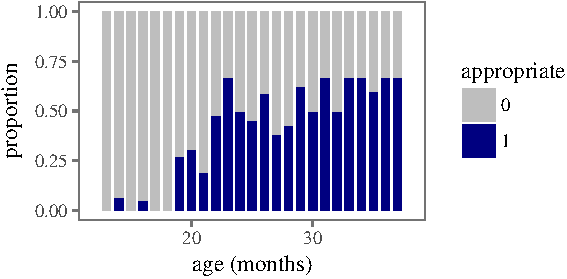
\includegraphics{figs/answerHitsPlot-1} 

}

\caption{Proportion of children's appropriate resonses}\label{fig:answerHitsPlot}
\end{figure}
\subsection{Discussion}\label{discussion-4}

The goal of this study was to discover the potential cues in
child-directed speech that could help children learn the interpretations
of \emph{and} and \emph{or}. The study presented 1000 examples of
\emph{and} and \emph{or} in child-directed speech, annotated for their
truth-conditional interpretation, as well as five candidate cues to
their interpretation: (1) Utterance Type; (2) Intonation Type; (3)
Syntactic Level; (4) Conceptual Consistency; (5) Communicative Function.
Like Morris (2008), this study found that the most common
interpretations of \emph{and} and \emph{or} are conjunction AND and
exclusive disjunction XOR. When the data were broken down by the
connectives, \emph{and} was almost always interpreted as a conjunction
while \emph{or} received three main interpretations: exclusive
disjunction XOR, inclusive disjunction IOR, and conjunction AND.

While the most frequent interpretation of \emph{or} was exclusive XOR
overall followed by IOR, the distribution of disjunction interpretations
shifted when they were broken down by the cues identified here. A
disjunction was most likely exclusive if the alternatives were
inconsistent (i.e.~contradictory). A disjunction was most likely
exclusive if it appeared in a question. Within questions, a disjunction
was most likely exclusive if the intonation was rise-fall. If the
intonation was rising, the question was interpreted as inclusive. The
syntactic category of the disjuncts could also provide information for
interpretation. If the disjuncts were clausal then it was more likely
for the disjunction to be interpreted as exclusive, even though this
effect was small. Finally, specific communicative functions required
specific interpretations of the connective. \emph{or} often received a
conjunctive interpretation in the following contexts: defining terms and
providing examples, enumerating options, and in unconditional
constructions. These results suggest that in order to successfully learn
to interpret a disjunction, children need to pay attention to a wide
variety of formal and conceptual factors.

In order to have a rough measure of children's comprehension of
disjunction, this study also investigated the types of answers they
provided to polar questions with disjunction. Between the ages of 20 and
30 months (roughly 1;6 to 2;6 years), children start to answer \emph{or}
questions appropriately. They would respond to a yes/no question such as
``do you want any apple juice or orange juice?'' with a yes/no answer.
They would also respond to an alternative question, as in``do you want
to play inside or outside?'', with one of the alternates, e.g.
``inside''. This finding is consistent with the first corpus study
presented in this chapter, which reported that the age range between 1;6
and 4 is the age range in which children develop their understanding of
\emph{and} and \emph{or}.

Due to the exploratory nature of this study, it is important to
replicate and extend these results and conclusions in future studies.
For example, future studies could use an automated procedure for the
annotation of categories such as utterance type, syntactic level, and
intonation. An automated procedure would also allow for the annotation
of larger samples and so could result in more reliable estimates for the
role of various factors in learning the meanings of function words. For
categories such as communicative function and connective interpretation,
future studies could use a larger number of independent annotators to
increase the speed and number of annotations. However, several results
reported in this study are independently supported by previous research.
Morris (2008) found similar results with respect to the overall
interpretation of disjunction in child-directed speech: \emph{and} is
most often interpreted as conjunction and \emph{or} as exclusive
disjunction. In an experimental study, Pruitt \& Roelofsen (2013) have
shown that a rise-fall intonation results in an exclusive
interpretation. Geurts (2006) has argued that a portion of exclusivity
inferences are simply due to the fact that the alternatives are mutually
exclusive and inconsistent.

Finally, the list of cues investigated here is in no way exhaustive.
There are at least two additional, possibly important factors/cues that
I set aside due to the difficulties that their annotation would have
introduced. First, an exclusive interpretation is sometimes the result
of a presupposition that only one alternative can hold or would matter
for the purposes of the conversation. For example, in the context of a
class activity where students pair up, a statement such as ``Lisa worked
with Ann or John'' is interpreted as exclusive simply because the
context already presupposes that only one disjunct can be true. Second,
some exclusivity inferences are due to the speaker's choice of
connective, namely using \emph{or} rather than \emph{and}. Grice (1989)
famously argued that in some cases, we interpret a disjunction like
\emph{A or B} as A or B, but not both because we reason that if the
speaker intended to communicate that both alternatives hold, s/he would
have said \emph{A and B}. This study did not annotate for such cases.
However, the study's results suggest that such cases of exclusive
interpretations are less frequent in child-directed speech that the ones
already annotated for. Investigating how often such cases of pragmatic
exclusion appear in child-directed speech can help us better understand
the role of input in children's acquisition of scalar implicatures.

\section{Conclusion}\label{conclusion-1}

This chapter presented two studies on the frequency and usage of
\emph{and} and \emph{or}. The first study looked at the frequencies of
these two words in a large collection of corpora for children between
the ages of 1 and 6 years. It showed that children start producing
\emph{and} between 12 to 18 months of age and rapidly increase their
productions until they reach the adult rate at 30 months. The production
of \emph{or} starts a little later, between 18-30 months, and rapidly
reaches a steady rate at 48 months. This rate is below the adult rate
for \emph{or} in child directed speech. The results suggest we can
expect an early understanding of disjunction between the ages of 18 and
30 months.

The second study looked at the interpretations of \emph{and} and
\emph{or} in a sample of child directed speech, as well as the cues that
accompany these instances. The study confirmed preivous finding that
exclusive disjunciton is the most common interpretation of \emph{or} in
child directed speech. However, the also found that exclusive
interpretations are reliably cued by intonation and the consistency of
the disjuncts. In the absence of these cues, a disjunction is most
likely inclusive or conjunctive. In the next chapter, I provide a
computational model that uses the cues discussed here to learn the
interpretation of utterances containing \emph{and} and \emph{or}.

\chapter{Learning disjunction from multiple cues}\label{modeling}

\section{Introduction}\label{introduction-4}

In Chapter \ref{sempragLit}, I reviewed the complexities involved in
interpreting a disjunction word such as \emph{or} in English. I showed
that a disjunction can be interpreted as inclusive, exclusive, and even
conjunctive. In adition to these truth-conditional interpretations, a
disjunction is sometimes associated with speaker ignorance/indifference
as well. Given the wide range of interpretations that \emph{or} can
have, how can children learn to interpret it correctly? In Chapter
\ref{devoLit}, I presented the results of Morris (2008) that suggested
children rarely hear the word \emph{or}; and when they do, they largely
hear the exclusive interpretation (75-80\% of the time). The annotation
study of Chapter \ref{corpus} replicated Morris (2008)'s finding. In
Chapter \ref{devoLit}, I also reported the results of recent
comprehension studies that show children between the ages of three and
five interpret \emph{or} as inclusive disjunction (Crain, 2012). Chapter
\ref{comprehension} confirmed that children between three and five can
interpret \emph{or} as inclusive in simple existential sentences. The
finding of the comprehension studies and the corpus studies taken
together present a learning puzzle: how can children learn to interpret
\emph{or} as inclusive if they mostly hear exclusive examples? This
chapter provides a solution by developing a cue-based account for
children's acquisition of connectives. More generally, the account
proposed in this chapter is helpful for learning words with multiple
interpretations when one interpretation dominates the learner's input.

Learning from multiple cues is a common approach in language acquisition
(See Monaghan \& Christiansen, 2014 for an overview). In the domain of
function word semantics, Wynn (1992) proposed a cue-based account for
the acquisition of number words. In the next section, I briefly review
their proposal and report their findings. The annotation study in
Chapter @\ref(corpus) used a methodology similar to that of Wynn (1992)
and reported several cues that can help children's acquisition of the
connectives \emph{and}/\emph{or}. In this section, I use the data in my
annotation study to present a cue-based account of connective
acquisition. This account provides a straightforward solution to the
learning puzzle of disjunction. I support this claim using three
modeling experiments that incorporate the proposed cues to learn
decision trees that predict the interpretation of a
disjunciton/conjunction with high accuracy. I end the chapter with a
discussion of the assumptions and limitations of the proposed account.

\section{The Cue-based Account for Number
Words}\label{the-cue-based-account-for-number-words}

Research on children's acquisition of numeral words (e.g. \emph{one},
\emph{two}, \emph{three}, etc.) has suggested that children initially
know that number words more than ``one'' refer to precise numerosities
but they do not know exactly which number refers to which word (Wynn,
1992). P. Bloom \& Wynn (1997) searched for linguistic cues that could
help children associate numerals with quantity and numerosity. They
considered two classes of cues: syntactic and semantic. Syntactic cues
to word meaning were first discussed by R. W. Brown (1957). He wrote:
``If a part of speech has reliable semantic implications, it could call
attention to the kind of attribute likely to belong to the meaning of
the word \ldots{} the part of speech memebership of the new word could
operate as a filter selecting for attention probably relevant features
of the nonlinguistic world.'' He tested preschoolers with nonce
constructions ``to sib'', ``a sib'', and ``any sib'' showing that
children can use the modifying function words to decide witheher the
nonce word \emph{sib} should refer to an action, an object, or a
substance.

Semantics cues, on the other hand, are provided by the meaning of the
known words in the sentence. Consider the sentence ``there were several
gloobs.'' The use of \emph{gloob} in the plural noun phrase ``several
gloobs'' makes it possible to infer that ``gloob'' is not an action or a
spatial relationship but rather an entity that can have multiple
instances. Using only the syntactic cues, there still remains a wide
range of referential uncertainty since a gloob may be anythign from an
egg to an alien creature. Now consider the sentence ``I ate several
gloobs for breakfast.'' What a gloob may be is now restricted to edible
entities, probably those that are suitable for breakfast. The meanings
of the verb \emph{eat} and the adverbial phrase ``for breakfast'' help
us further narrow down the possible meaning for \emph{gloob}.

It is not always easy to tell whether a cue is syntactic or semantic.
Here I avoid this issue by using the term ``compositional cues'' to
refer to both syntactic and semantic cues that aid the interpretation of
an unknown word. Using the term ``compositional'' also brings into
attention the fact that syntactic and semantic cues are interrelated and
do not act in a an independent or unstructured way. Consider the
sentence ``After eating breakfast, I saw several gloobs.'' Even though
the words \emph{eat} and \emph{breakfast} are present in the sentence,
they do not restrict the possible meanings for \emph{gloob} as they did
before. In other words, it is not the mere presence of these words in
the sentence that act as cues but rather the way they combine with the
unknown word to convey the main communicative message of the utterance.

P. Bloom \& Wynn (1997) proposed that children learn number word
meanings by attending to the compositional cues that accompany number
words such as the words' ordering relative to other words, other
funciton words they co-occur with, and the count-mass status of the
nouns they modify. They specifically discussed four cues. Two cues could
help children notice that number words pattern like quantifiers. First,
similar to quantifiers, number words precede adjectives and do not
follow them. Second, they participate in the ``\ldots{} of the Xs''
construction: ``one of the gloobs'', ``some of the gloobs'', ``most of
the gloobs'', etc. The third cue is the co-occurrence of number words
with count nouns. This cue can inform learners that their meaning is
restricted to the quantification of individuals. Finally, unlike other
adjectives, numerals cannot be modified further using an adverb such as
\emph{very} or \emph{too} (``very big animals'' vs.
``\textbackslash{}*very two animals``). According to P. Bloom \& Wynn
(1997), this cue can help a learner understand that number words pick an
absolute property of a set rather than a continuous one.

Using the data available in the CHILDES corpora,
\href{mailto:corpora@bloom1997linguistic}{\nolinkurl{corpora@bloom1997linguistic}}
investigated the presence of cues to number word emaning in chlild
directed speech for three children between the ages of one and three.
They found that these children and their parents only use number words
with count nouns. They do not use number words with modifiers and only
use them before adjectives; not after. Finally, they found that these
children and their parents use only number words and quantifiers in the
partitive construction and not adjectives. The results of their corpus
study shows that the compositional cues they proposed for number word
acquisition are available in children's linguistic input.

The issues in the development of disjunction are quite similar to those
in the development of number words. Similar to number words, previous
research has provided insight into how children comprehend a disjunction
and what they hear from their parents. The main questions is how
children learn what they comprehend from what they hear. I turn to this
issue in the next section.

\section{\texorpdfstring{Learning \emph{and}/\emph{or}: A cue-based
account}{Learning and/or: A cue-based account}}\label{myaccount}

Previous comprehension studies as well as the one reported in Chapter
\ref{comprehension} have shown that children as early as age three can
interpret a disjunction as inclusive. However, studies of child-directed
speech like the one in Chapter \ref{corpus} have shown that exclusive
interpretations dwarf other interpretations of disjunction in children's
input. How can children learn the inclusive interpretation of a
disjunction when the majority of the examples they hear are exclusive?
To answer this question, I draw insight from the Gricean approach to
semantics and pragmatics discussed in Chapter \ref{sempragLit}.

Research in Gricean semantics and pragmatics has shown that the word
\emph{or} is not the only factor relevant to the interpretation of a
disjunction. It is not only the presence of the word \emph{or} that
makes us interpret a disjunction as inclusive, exclusive, or
conjunctive, but rather the presence of \emph{or} along with several
interpretive factors such as intonation (Pruitt \& Roelofsen, 2013), the
meaning of the disjuncts (Geurts, 2006), and the conversational
principles governing communication (Grice, 1989). Therefore,
interpretation and acquisition of the word \emph{or} cannot be separated
from all the factors that accompany it and shape the final
interpretation of a disjunciton.

In the literature on word learning and semantic acquisition,
form-meaning mapping is construed as mapping an isolated form such as
\emph{gavagai} to an isolated concept such as ``rabbit''. While this
approach may be feasible for content words, it will not work for
function words such as \emph{or}. First, the word \emph{or} cannot be
mapped isolated from its formal context. As Pruitt \& Roelofsen (2013)
showed, the intonation that accompanies a disjunction affects its
interpretation. Therefore, a learner needs to pay attention to the word
\emph{or} as well as the intonation contour that accompanies it. Second,
the word \emph{or} cannot be mapped to its meaning isolated from the
semantics of the disjuncts that accompany it. As Geurts (2006) argued,
the exclusive interpretation is often enforced simply because the
options are incompatible. For example, ``to be or not to be'' is
exclusive simply because one cannot both be and not be! In addition,
conversational factors play an important role in the interpretation of
\emph{or} as Grice (1989) argued as well. In sum, the interpretation and
acquisition of function words such as \emph{or} require the learner to
consider the linguistic and nonlinguistic context of the word and map
the meaning of the word accordingly.

Previous accounts have tacitly adopted a model in which a function word
such as \emph{or} is mapped to its most common interpretation: \emph{or}
\(\rightarrow \oplus\). Here I argue that the direct mapping of
\emph{or} to its interpretation without consideration of its linguistic
context is the primary cause of \emph{or}'s learning puzzle. Instead, I
propose that the word \emph{or} is mapped to an interpretation along
with the interpretive cues that accompany it such as intonation and
disjunct semantics:

{[}connective: \emph{or}, Intonation: rise-fall, Disjuncts:
inconsistent{]} \(\rightarrow \oplus\)

{[}connective: \emph{or}, Intonation: rising, Disjuncts: consistent{]}
\(\rightarrow \lor\)

In this account, it is not a single word that gets mapped to an
interpretation but rather a cluster of features. This method has two
advantages. First, it deals with the context dependency of disjunction
interpretation. The learner knows that \emph{or} with some intonation
has to be interpreted differently from one with another. Second, it
allows the learner to pull apart the contribution of \emph{or} from the
interpretive cues that often accompany it. In fact, analysis of all
mapping clusters in which \emph{or} participates and generalization over
them can help the learner extract the semantics of \emph{or} the way it
is intended by Gricean semanticists. For those skeptical of such an
underlying semantics for \emph{or}, there is no need for further
analysis of the mapping clusters and the meaning of \emph{or} as a
single lexical item is distributed among the many mappings in which it
participats. In the next section, I implement this idea using decition
tree learning.

\section{Modeling}\label{modeling}

Introduction to decision trees

In the following subsections, we present three different stages of our
modeling. First we used decision trees to predict whether a disjunction
is exclusive or not. The second model incorporates both conjunction and
disjunction and distinguishes between inclusive, exclusive, and
conjunctive interpretations. The third model includes all
interpretations in the annotation study as well as all the features the
examples were annotated for.

\subsection{Learning Exclusivity}\label{learning-exclusivity}

\subsubsection{Methods}\label{methods-4}

To understand the acquisition and interpretation of exclusive
inferences, we grouped our interpretation annotations into two
categories: Exclusive and Inclusive. Exclusive interpretations consisted
of the EX category (exclusive) and NAB (the first disjunct is false and
the second true/intended). We counted other categories as inclusive
(IN). First, similar to Morris (2008), we found that the majority of
\emph{or} examples in CDS receive an exclusive interpretation
(\(\sim\)\%65). Figure \ref{fig:interpretation} shows this difference in
distribution. As shown in Study 2 of Chapter \ref{corpus}, the rate of
exclusive interpretations change systematically when we break the data
down by intonation and consistency (Figure
\ref{fig:interpretationByIntonationAndConsistency}). Given a rise-fall
intonation contour, a disjunction is almost always interpreted as
exclusive. Similarly, if the propositions are inconsistent, the
disjunction is most likely interpreted as exclusive. When either of
these two features are absent, a disjunction is more likely to receive
an inclusive interpretation.

We fit a mixed-effects binomial logistic regression using the package
\{lme4\} (Bates, Maechler, Bolker, Walker, \& others, 2014) in R with
fixed effects of intonation and consistency as well as random intercepts
for children. Both intonation and consistency were significant
predictors of exclusivity. Disjunctions were more likely to be
interpreted as exclusive if they received a rise-fall intonation
(\(\beta\)=-3.75, \(z\)=-8.49, \(p < 0.001\)) or if they were
inconsistent (\(\beta\)=-2.17, \(z\)=-8, \(p < 0.001\)). Disjunctions
were more likely to be interpreted as inclusive if they were consistent
and received a rising (\(\beta\)=0.67, \(z\)=2.44, \(p < 0.001\)) or
flat intonation (\(\beta\)=0.71, \(z\)=3.44, \(p < 0.001\)).

The analysis above suggested that intonation and consistency are helpful
in discerning exclusive and inclusive (non-exclusive) interpretations of
disjunction. To investigate how informative these patterns were more
quantitatively, we built a model to predict the interpretation of a
disjunction after training on examples annotated for intonation and
consistency. To more easily understand the rules governing exclusivity,
we fit a decision tree model using Sci-kit Learn's Decision Tree Module
(Pedregosa et al., 2011). We randomly sampled 100 examples for training
and 300 examples for testing.
\begin{itemize}
\tightlist
\item
  AKSHAY: more explanation on the model assumptions and parameters
\end{itemize}
\subsubsection{Results}\label{results-4}
\begin{figure}[b]

{\centering 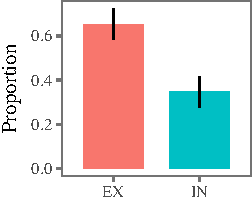
\includegraphics{figs/interpretation-1} 

}

\caption{Proportion of exclusive and inclusive interpretations of disjunction in child-directed speech. Error bars represent bootstrapped 95\% confidence intervals.}\label{fig:interpretation}
\end{figure}
\begin{figure}[t]

{\centering 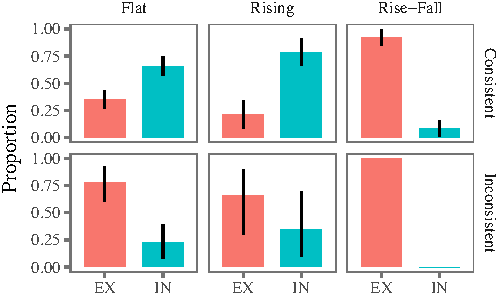
\includegraphics{figs/interpretationByIntonationAndConsistency-1} 

}

\caption{Exclusive and inclusive interpretations broken down by intonation (flat, rise, rise-fall) and consistency. Error bars represent bootstrapped 95\% confidence intervals.}\label{fig:interpretationByIntonationAndConsistency}
\end{figure}
\begin{figure}[tb]

{\centering 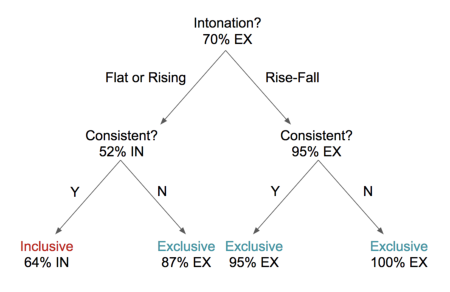
\includegraphics{figs/treeDiagram-1} 

}

\caption{Optimal decision tree training on 100 datapoints. Provides series of two binary decisions to decide exlcusivity interpretation. Intonation $>$ 1.5 are rise-fall while intonation $<$ 1.5 are flat or rising. Consistency $>$ 0.5 are consistent while consistency $<$ 0.5 are  inconsistent.}\label{fig:treeDiagram}
\end{figure}
Averaged over 100 trials, the average accuracy of a binary tree was
83\%. More remarkably, the tree achieved an average of 80\% accuracy
after training on only 20 examples (Figure \ref{fig:learningCurve}). The
control flow of the average decision tree on a single example is as
follows. If \emph{or} has neither rise-fall nor inconsistent disjuncts,
it is marked inclusive. Otherwise, exclusive (Figure
\ref{fig:treeDiagram}). The success of such a simple decision-tree
indicates that children could use a simple model to rapidly learn the
exclusive interpretation of \emph{or} from infrequent data.
\begin{figure}[tb]
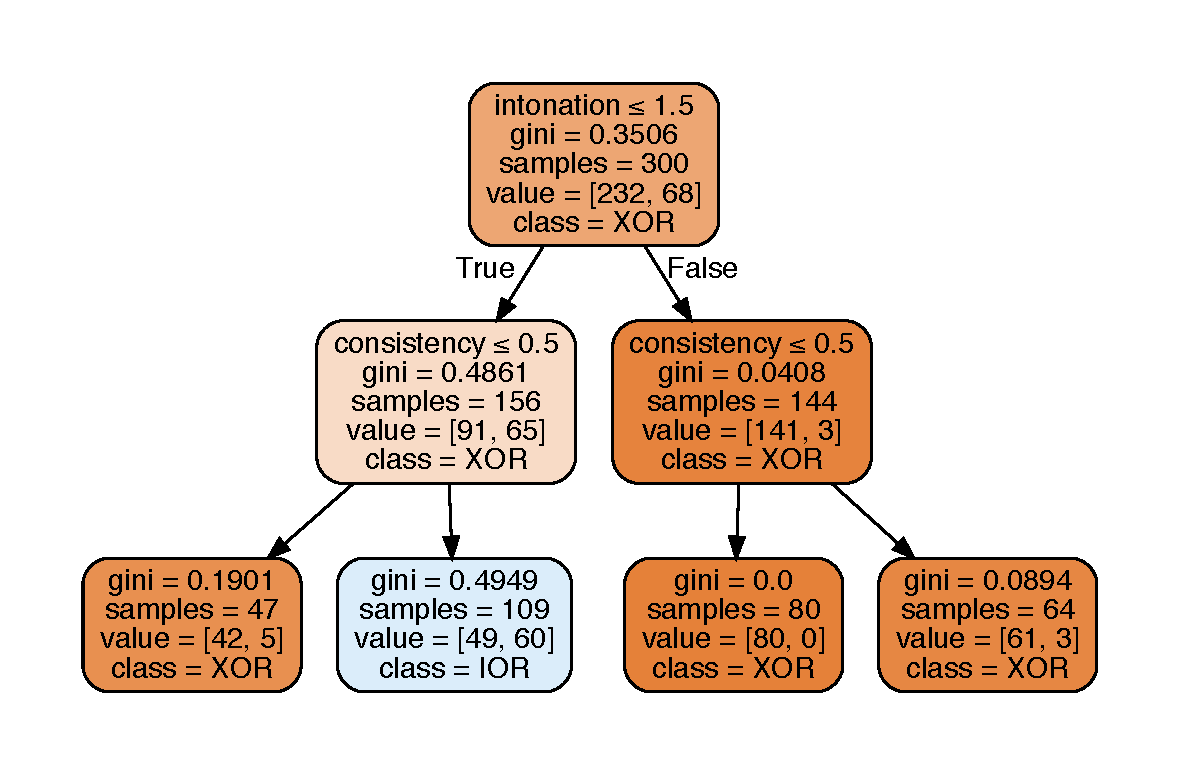
\includegraphics[width=0.6\linewidth]{decision_trees/plots/exin} \caption{A caption}\label{fig:exorTree}
\end{figure}
\begin{figure}[tb]

{\centering 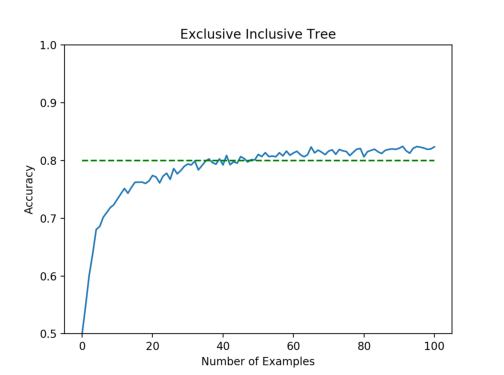
\includegraphics{figs/exorLearning-1} 

}

\caption{Laerning Curve for Exclusive interpretations.}\label{fig:exorLearning}
\end{figure}
\subsection{Learning Exclusive, Inclusive and Conjunctive
Interpretations}\label{learning-exclusive-inclusive-and-conjunctive-interpretations}

This section includes the annotation data on \emph{and} as well as
\emph{or} and uses decision trees to predict three different
interpretations: inclusive, exclusive, and conjunctive.

\subsubsection{Methods}\label{methods-5}

\subsubsection{Results}\label{results-5}

From 300 annotated examples labeled IOR, XOR, or AND, we use intonation,
speech act, consistency, and annotation to separate them. \newline

If Annotation is AND, AND \newline
If intonation is rise-fall, XOR \newline
If intonation is rising and inconsistent, XOR \newline
If intonation is rising and consistent, IOR \newline
If intonation is flat and speech act options/defex/unconditional, AND
\newline
If intonation is flat and other speech act, XOR \newline
\begin{figure}[tb]
\includegraphics[width=0.9\linewidth]{decision_trees/plots/exinand} \caption{A caption}\label{fig:exinandTree}
\end{figure}
\begin{figure}[tb]

{\centering \includegraphics{figs/exinandLearning-1} 

}

\caption{Laerning Curve for Exclusive, Inclusive, and Conjunctive interpretations.}\label{fig:exinandLearning}
\end{figure}
\section{Learning All Annotated
Interpretations}\label{learning-all-annotated-interpretations}

\subsection{Methods}\label{methods-6}

\subsection{Results}\label{results-6}

From 300 annotated examples labeled IOR, XOR, AND, NPQ, XNOR, or NOR, we
use intonation, speech act, consistency, utterance type, and annotation
to separate them. \newline

If Annotation is AND, AND \newline
IF intonation is rise-fall, XOR \newline
If intonation is rising and inconsistent, XOR \newline
If intonation is rising and consistent, IOR \newline
If intonation is flat and speech act is (unconditional or repair or
directive description), NPQ \newline
If intonation is flat and speech act is defex, AND \newline
If intonation is flat and speech act is (conditional, identification,
clarification, or directive), XOR \newline
If intonation is flat and speech act is (description, options,
preference), ??? \newline
\begin{figure}[tb]
\includegraphics[width=0.9\linewidth]{decision_trees/plots/everything} \caption{A caption}\label{fig:everyTree}
\end{figure}
\begin{figure}[tb]

{\centering \includegraphics{figs/everythingLearning-1} 

}

\caption{Laerning Curve for Exclusive, Inclusive, and Conjunctive interpretations.}\label{fig:everythingLearning}
\end{figure}
\section{Discussion}\label{discussion-5}
\begin{itemize}
\item
  Summary
\item
  The solution proposed in this chapter can be more generally applied to
  learn relatively infrequent interpretations or usages of words.
  However, the account fails if there are no interpretive cues for the
  intended interpretation or usage.
\item
  The proposed account allows for both Gricean and ambguity approaches
  to semantics to have a developmental story.
\end{itemize}
It is important to be explicit about the assumptions and the limitations
of the account described in this chapter. First the account assumes that
the learner limits the hypothesis space to a small set of binary logical
connectives. This is no simple task and it is important to investigate
what constraints or cues can help it. A viable option is to rely on the
peculiar syntactic properties of coordination. The literature on
syntactic bootstrapping suggests that children can use syntactic
bootstrapping to limit their word meaning hypotheses to the relevant
domain. A coordinator such as \emph{and}/\emph{or} conjoins similar
syntactic categories: two sentences, two verbs, or two nominals. This is
not a common pattern for other functional elements and syntactic
theories posit specific rules for coordination. It is possible that the
special syntactic status of coordinators can cue their meaning and help
the learner distinguish them from other types of function words.

Within binary logical meanings , it is reasonable to assume that not all
binary meanings are as likely for mapping.
\begin{itemize}
\tightlist
\item
  ruling out conjunction for the meaning of \emph{or} using consistency
  of the disjuncts
\end{itemize}
Semantic properties of the coordinands can help children distinguish the
meaning of \emph{and} and \emph{or}. While \emph{or} appears with both
consistent and inconsistent coordinands, \emph{and} only appears with
consistent coordinands. Therefore, conjunction is not a viable
hypothesis for the meaning of \emph{or}.

A major limitation of the model is that it only from about 500 data
points. This is substantially fewer number of examples than what
children hear until they reach the age of 3. It is reasonable to expect
that the model's performance, especially for conjunctive and negative
(NOR) interpretations improves with more example data that allows the
model to learn the features that correlate systematically with uncommon
interpretations.

Explain how much you expect these to generalize to other connective
words or more generally function words.

It is also important to think about the role of attention in learning.
Currently models assume that each example has equal siginficance to
learning and the learner pays equal attention to them. This does not
match the intuitive understanding of learning. We dedicate more
resources and attention to tasks we have not yet mastered while skills
or knowledge we already possess becomes part of the daily routine and we
do not need to assign learning resources to them.

In the case of conjunction and disjunction, a large part of the input is
very similar and repetetive. Children can learn their meaning and
structure quickly and future exmples are not informative or challenging.
It is reasonable to assume that children dedicate their resources to the
more challenging instances and focus on mastering them. In such a model,
learning is surprisal driven. If a usage is novel and unfamiliar, the
learner assigns more learning resources to it and focuses on learning
them. This way, the learner can move from extremely frequent instances
in the input to the rare ones. Under such a model, frequency determines
order of acquisition (to some degree) but not whether a construction is
learned or not. Under the right circumstances even a one time occurance
of a word or construction can result in successful learning.

\chapter{Conclusion}\label{conclusions}

Talk about claims of innateness maybe? Are logical concepts innate? are
they any more special than size etc.?

I asked what constraints and cues aid children's acquisition of function
words?

The general account: Syntactic bootstrapping constrains the hypothsis
space for the function word. Cues such as intonation, semantics of the
content words being combined, the communicative function of the
sentence, etc. help the learner in mapping the function word to its
meaning.

In case of disjunction: Syntactic bootstrapping constrains the
hypothesis space to the connective meanings. ``syntactic constructions
in which two or more units of the same type are combined into a larger
unit and still have the same semantic relations with other surrounding
elements.'' Intonation, disjunct semantics
\begin{itemize}
\tightlist
\item
  The role of ruotines and common conceptual representations in learning
  the meaning of function words.
  \begin{itemize}
  \tightlist
  \item
    Eve's work on spatial prepositions of in/on/under
  \item
    Eve's work on temporal connectives before and after
  \item
    Bloom's work on number words
  \item
    Piantedosi et al on quantifier learning
  \end{itemize}
\item
  Forming interpretations at the top level based on the routines,
  mapping at the top level, then breaking them down to retrieve word
  meaning consistent across constructions
\item
  However, mapping should take into account the formal and conceptual
  environment of mapping
\end{itemize}
\chapter*{References}\label{references}
\addcontentsline{toc}{chapter}{References}

\markboth{References}{References}

\noindent

\setlength{\parindent}{-0.20in} \setlength{\leftskip}{0.20in}
\setlength{\parskip}{8pt}

\hypertarget{refs}{}
\hypertarget{ref-akhtar1999acquiring}{}
Akhtar, N. (1999). Acquiring basic word order: Evidence for data-driven
learning of syntactic structure. \emph{Journal of Child Language},
\emph{26}(02), 339--356.

\hypertarget{ref-Aloni2016}{}
Aloni, M. (2016). Disjunction. In E. N. Zalta (Ed.), \emph{The stanford
encyclopedia of philosophy}. Stanford University. Retrieved from
\url{https://plato.stanford.edu/archives/win2016/entries/disjunction/}

\hypertarget{ref-Ariel2014}{}
Ariel, M. (2014). Or constructions: Monosemy vs. polysemy. In B.
MacWhinney, A. Malchukov, \& E. Moravcsik (Eds.), \emph{Competing
motivations in grammar and usage}. Oxford University Press.

\hypertarget{ref-baldwin1993infants}{}
Baldwin, D. A. (1993). Infants' ability to consult the speaker for clues
to word reference. \emph{Journal of Child Language}, \emph{20}(2),
395--418.

\hypertarget{ref-barner2011accessing}{}
Barner, D., Brooks, N., \& Bale, A. (2011). Accessing the unsaid: The
role of scalar alternatives in children's pragmatic inference.
\emph{Cognition}, \emph{118}(1), 84--93.

\hypertarget{ref-barner2009finding}{}
Barner, D., Chow, K., \& Yang, S.-J. (2009). Finding one's meaning: A
test of the relation between quantifiers and integers in language
development. \emph{Cognitive Psychology}, \emph{58}(2), 195--219.

\hypertarget{ref-bates2014lme4}{}
Bates, D., Maechler, M., Bolker, B., Walker, S., \& others. (2014).
Lme4: Linear mixed-effects models using eigen and s4. \emph{R Package
Version}, \emph{1}(7), 1--23.

\hypertarget{ref-beilin1975study}{}
Beilin, H., \& Lust, B. (1975). A study of the development of logical
and linguistics connectives: Linguistics data. \emph{Studies in the
Cognitive Basis of Language Development}, 76--120.

\hypertarget{ref-berwick1985acquisition}{}
Berwick, R. C. (1985). \emph{The acquisition of syntactic knowledge}.
MIT press.

\hypertarget{ref-bloom1997linguistic}{}
Bloom, P., \& Wynn, K. (1997). Linguistic cues in the acquisition of
number words. \emph{Journal of Child Language}, \emph{24}(3), 511--533.

\hypertarget{ref-gabbay2012logic}{}
Bonevac, D., \& Dever, J. (2012). A history of the connectives. In D. M.
Gabbay, F. J. Pelletier, \& J. Woods (Eds.), \emph{Logic: A history of
its central concepts} (Vol. 11). Newnes.

\hypertarget{ref-braine1981development}{}
Braine, M. D., \& Rumain, B. (1981). Development of comprehension of
``or'': Evidence for a sequence of competencies. \emph{Journal of
Experimental Child Psychology}, \emph{31}(1), 46--70.

\hypertarget{ref-brown1957linguistic}{}
Brown, R. W. (1957). Linguistic determinism and the part of speech.
\emph{The Journal of Abnormal and Social Psychology}, \emph{55}(1), 1.

\hypertarget{ref-chierchia2013logic}{}
Chierchia, G. (2013). \emph{Logic in grammar: Polarity, free choice, and
intervention}. OUP Oxford.

\hypertarget{ref-chierchia1998some}{}
Chierchia, G., Crain, S., Guasti, M. T., \& Thornton, R. (1998).
``Some'' and ``or'': A study on the emergence of logical form. In
\emph{Proceedings of the boston university conference on language
development} (Vol. 22, pp. 97--108). Cascadilla Press Somerville, MA.

\hypertarget{ref-chierchia2001acquisition}{}
Chierchia, G., Crain, S., Guasti, M. T., Gualmini, A., \& Meroni, L.
(2001). The acquisition of disjunction: Evidence for a grammatical view
of scalar implicatures. In \emph{Proceedings of the 25th boston
university conference on language development} (pp. 157--168).
Cascadilla Press Somerville, MA.

\hypertarget{ref-chierchia2004semantic}{}
Chierchia, G., Guasti, M. T., Gualmini, A., Meroni, L., Crain, S., \&
Foppolo, F. (2004). Semantic and pragmatic competence in children's and
adults' comprehension of or. In \emph{Experimental pragmatics} (pp.
283--300). Springer.

\hypertarget{ref-cicchetti1990high}{}
Cicchetti, D. V., \& Feinstein, A. R. (1990). High agreement but low
kappa: II. resolving the paradoxes. \emph{Journal of Clinical
Epidemiology}, \emph{43}(6), 551--558.

\hypertarget{ref-clark1987principle}{}
Clark, E. V. (1987). The principle of contrast: A constraint on language
acquisition. \emph{Mechanisms of Language Acquisition}, \emph{1}, 33.

\hypertarget{ref-clark1993lexicon}{}
Clark, E. V. (1993). \emph{The lexicon in acquisition}. Cambridge
University Press.

\hypertarget{ref-clark2009first}{}
Clark, E. V. (2009). \emph{First language acquisition}. Cambridge
University Press.

\hypertarget{ref-clark1993computational}{}
Clark, R., \& Roberts, I. (1993). A computational model of language
learnability and language change. \emph{Linguistic Inquiry},
\emph{24}(2), 299--345.

\hypertarget{ref-crain1991language}{}
Crain, S. (1991). Language acquisition in the absence of experience.
\emph{Behavioral and Brain Sciences}, \emph{14}(04), 597--612.

\hypertarget{ref-crain2008interpretation}{}
Crain, S. (2008). The interpretation of disjunction in universal
grammar. \emph{Language and Speech}, \emph{51}(1-2), 151--169.

\hypertarget{ref-crain2012emergence}{}
Crain, S. (2012). \emph{The emergence of meaning}. Cambridge University
Press.

\hypertarget{ref-crain2008logic}{}
Crain, S., \& Khlentzos, D. (2008). Is logic innate?
\emph{Biolinguistics}, \emph{2}(1), 024--056.

\hypertarget{ref-crain2010logic}{}
Crain, S., \& Khlentzos, D. (2010). The logic instinct. \emph{Mind \&
Language}, \emph{25}(1), 30--65.

\hypertarget{ref-crain1998investigations}{}
Crain, S., \& Thornton, R. (1998). \emph{Investigations in universal
grammar: A guide to experiments on the acquisition of syntax and
semantics}. MIT Press.

\hypertarget{ref-crain1999methodology}{}
Crain, S., \& Wexler, K. (1999). Methodology in the study of language
acquisition: A modular approach. \emph{Handbook of Child Language
Acquisition}, 387--425.

\hypertarget{ref-crain2000acquisition}{}
Crain, S., Gualmini, A., \& Meroni, L. (2000). The acquisition of
logical words. \emph{LOGOS and Language}, \emph{1}, 49--59.

\hypertarget{ref-crain1994learning}{}
Crain, S., Ni, W., \& Conway, L. (1994). Learning, parsing and
modularity. In C. Clifton, L. Frazier, \& K. Rayner (Eds.),
\emph{Perspectives on sentence processing} (pp. 443--467). Erlbaum
Hillsdale.

\hypertarget{ref-demuth2006word}{}
Demuth, K., Culbertson, J., \& Alter, J. (2006). Word-minimality,
epenthesis and coda licensing in the early acquisition of english.
\emph{Language and Speech}, \emph{49}(2), 137--173.

\hypertarget{ref-feinstein1990high}{}
Feinstein, A. R., \& Cicchetti, D. V. (1990). High agreement but low
kappa: I. the problems of two paradoxes. \emph{Journal of Clinical
Epidemiology}, \emph{43}(6), 543--549.

\hypertarget{ref-fleiss2013statistical}{}
Fleiss, J. L., Levin, B., \& Paik, M. C. (2013). \emph{Statistical
methods for rates and proportions}. John Wiley \&amp; Sons.

\hypertarget{ref-ford1976language}{}
Ford, W. G. (1976). \emph{The language of disjunction} (PhD thesis).
University of Toronto.

\hypertarget{ref-fox2007free}{}
Fox, D. (2007). Free choice and the theory of scalar implicatures. In
\emph{Presupposition and implicature in compositional semantics} (pp.
71--120). Springer.

\hypertarget{ref-gazdar79}{}
Gazdar, G. (1979). \emph{Pragmatics: Implicature, presupposition, and
logical form}. Academic Press, New York.

\hypertarget{ref-geis1971invited}{}
Geis, M. L., \& Zwicky, A. M. (1971). On invited inferences.
\emph{Linguistic Inquiry}, \emph{2}(4), 561--566.

\hypertarget{ref-geurts2005entertaining}{}
Geurts, B. (2005). Entertaining alternatives: Disjunctions as modals.
\emph{Natural Language Semantics}, \emph{13}(4), 383--410.

\hypertarget{ref-geurts2006exclusive}{}
Geurts, B. (2006). Exclusive disjunction without implicatures.
\emph{Ms., University of Nijmegen}.

\hypertarget{ref-geurts2010quantity}{}
Geurts, B. (2010). \emph{Quantity implicatures}. Cambridge University
Press.

\hypertarget{ref-giannakidou2011negative}{}
Giannakidou, A. (2011). Negative and positive polarity items: Variation,
licensing, and compositionality. \emph{Semantics: An International
Handbook of Natural Language Meaning. de Gruyter, Berlin (to Appear)}.

\hypertarget{ref-goodman2008does}{}
Goodman, J. C., Dale, P. S., \& Li, P. (2008). Does frequency count?
Parental input and the acquisition of vocabulary. \emph{Journal of Child
Language}, \emph{35}(3), 515--531.

\hypertarget{ref-goro2004acquisition}{}
Goro, T., \& Akiba, S. (2004). The acquisition of disjunction and
positive polarity in japanese. In \emph{Proceedings of the 23rd west
coast conference on formal linguistics} (pp. 251--264). Cascadilla Press
Summerville, MA.

\hypertarget{ref-grice1989studies}{}
Grice, H. P. (1989). \emph{Studies in the way of words}. Harvard
University Press.

\hypertarget{ref-gualminicrain2002}{}
Gualmini, A., \& Crain, S. (2002). Why no child or adult must learn de
morgan's laws. In \emph{Proceedings of the boston university conference
on language development}.

\hypertarget{ref-gualmini2000}{}
Gualmini, A., Crain, S., \& Meroni, L. (2000a). Acqisition of
disjunction in conditional sentences. In \emph{Proceedings of the boston
university conference on language development}.

\hypertarget{ref-gualmini2000inclusion}{}
Gualmini, A., Meroni, L., \& Crain, S. (2000b). The inclusion of
disjunction in child language: Evidence form modal verbs. In
\emph{Proceedings of the nels} (Vol. 30).

\hypertarget{ref-gutzmann2014}{}
Gutzmann, D. (2014). Semantics vs. pragmatics. In L. Matthewson, C.
Meier, H. Rullmann, \& T. E. Zimmermann (Eds.), \emph{The companion to
semantics}. Oxford: Wiley.

\hypertarget{ref-haspelmath2007}{}
Haspelmath, M. (2007). Coordination. In T. Shopen (Ed.), \emph{Language
typology and linguistic description,} Cambridge University Press.
Retrieved from \url{https://doi.org/10.1017/CBO9780511619434}

\hypertarget{ref-heeman1999speech}{}
Heeman, P. A., \& Allen, J. F. (1999). Speech repairs, intonational
phrases, and discourse markers: Modeling speakers' utterances in spoken
dialogue. \emph{Computational Linguistics}, \emph{25}(4), 527--571.

\hypertarget{ref-ho1995random}{}
Ho, T. K. (1995). Random decision forests. In \emph{Document analysis
and recognition, 1995., proceedings of the third international
conference on} (Vol. 1, pp. 278--282). IEEE.

\hypertarget{ref-hollich2000breaking}{}
Hollich, G. J., Hirsh-Pasek, K., Golinkoff, R. M., Brand, R. J., Brown,
E., Chung, H. L., \ldots{} Bloom, L. (2000). Breaking the language
barrier: An emergentist coalition model for the origins of word
learning. \emph{Monographs of the Society for Research in Child
Development}, i--135.

\hypertarget{ref-horn1989natural}{}
Horn, L. (1989). \emph{A natural history of negation}. University of
Chicago Press.

\hypertarget{ref-horn1972semantic}{}
Horn, L. R. (1972). On the semantic properties of logical operators in
english: University of california. \emph{Los Angeles PhD Dissertation}.

\hypertarget{ref-horowitz2017trouble}{}
Horowitz, A. C., Schneider, R. M., \& Frank, M. C. (2017). The trouble
with quantifiers: Exploring children's deficits in scalar implicature.
\emph{Child Development}.

\hypertarget{ref-piaget1958growth}{}
Inhelder, B., \& Piaget, J. (1958). \emph{The growth of logical thinking
from childhood to adolescence: An essay on the construction of formal
operational structures} (Vol. 84). Routledge.

\hypertarget{ref-johansson1977levels}{}
Johansson, B. S. (1977). Levels of mastery of the coordinators and and
or and logical test performance. \emph{British Journal of Psychology},
\emph{68}(3), 311--320.

\hypertarget{ref-johansson1975preschool}{}
Johansson, B. S., \& Sjölin, B. (1975). Preschool children's
understanding of the coordinators ``and'' and ``or''. \emph{Journal of
Experimental Child Psychology}, \emph{19}(2), 233--240.

\hypertarget{ref-kamp1973free}{}
Kamp, H. (1973). Free choice permission. In \emph{Proceedings of the
aristotelian society} (Vol. 74, pp. 57--74). JSTOR.

\hypertarget{ref-katsos2014scalar}{}
Katsos, N. (2014). Scalar implicature. In D. Matthews (Ed.),
\emph{Pragmatic development in first language acquisition} (Vol. 10).
John Benjamins Publishing Company.

\hypertarget{ref-katsos2011pragmatic}{}
Katsos, N., \& Bishop, D. V. (2011). Pragmatic tolerance: Implications
for the acquisition of informativeness and implicature.
\emph{Cognition}, \emph{120}(1), 67--81.

\hypertarget{ref-levy1994words}{}
Levy, E., \& Nelson, K. (1994). Words in discourse: A dialectical
approach to the acquisition of meaning and use. \emph{Journal of Child
Language}, \emph{21}(02), 367--389.

\hypertarget{ref-lieven1997lexically}{}
Lieven, E. V., Pine, J. M., \& Baldwin, G. (1997). Lexically-based
learning and early grammatical development. \emph{Journal of Child
Language}, \emph{24}(01), 187--219.

\hypertarget{ref-macwhinney1989competition}{}
MacWhinney, B. (1989). Competition and lexical categorization. In
\emph{Linguistic categorization} (pp. 195--242). John Benjamins,
Amsterdam.

\hypertarget{ref-macwhinney2000childes}{}
MacWhinney, B. (2000). \emph{The childes project: The database} (Vol.
2). Psychology Press.

\hypertarget{ref-macwhinney2002competition}{}
MacWhinney, B. (2002). The competition model: The input, the context,
and the brain. In P. Robinson (Ed.), \emph{Cognition and second language
instruction} (pp. 69--90). Cambridge University Press.

\hypertarget{ref-marcus1993negative}{}
Marcus, G. F. (1993). Negative evidence in language acquisition.
\emph{Cognition}, \emph{46}(1), 53--85.

\hypertarget{ref-markman1984children}{}
Markman, E. M., \& Hutchinson, J. E. (1984). Children's sensitivity to
constraints on word meaning: Taxonomic versus thematic relations.
\emph{Cognitive Psychology}, \emph{16}(1), 1--27.

\hypertarget{ref-markman1988children}{}
Markman, E. M., \& Wachtel, G. F. (1988). Children's use of mutual
exclusivity to constrain the meanings of words. \emph{Cognitive
Psychology}, \emph{20}(2), 121--157.

\hypertarget{ref-monaghan2014multiple}{}
Monaghan, P., \& Christiansen, M. (2014). Multiple cues in language
acquisition. \emph{Encyclopedia of Language Development}, 389--392.

\hypertarget{ref-morris2008logically}{}
Morris, B. J. (2008). Logically speaking: Evidence for item-based
acquisition of the connectives and \&amp; or. \emph{Journal of Cognition
and Development}, \emph{9}(1), 67--88.

\hypertarget{ref-neimark1970development}{}
Neimark, E. D., \& Slotnick, N. S. (1970). Development of the
understanding of logical connectives. \emph{Journal of Educational
Psychology}, \emph{61}(6p1), 451.

\hypertarget{ref-neisser1962hierarchies}{}
Neisser, U., \& Weene, P. (1962). Hierarchies in concept attainment.
\emph{Journal of Experimental Psychology}, \emph{64}(6), 640.

\hypertarget{ref-nitta1966basic}{}
Nitta, N., \& Nagano, S. (1966). Basic logical operations and their
verbal expressions: Child's conception of logical sum and product.
\emph{Research Bulletin of the National Institute for Educational
Research, Tokyo}.

\hypertarget{ref-notley2012notevery}{}
Notley, A., Thornton, R., \& Crain, S. (2012). English-speaking
children's interpretation of disjunction in the scope of ``not every''.
\emph{Biolinguistics}, \emph{6}(1), 32--69.

\hypertarget{ref-notley2012children}{}
Notley, A., Zhou, P., Jensen, B., \& Crain, S. (2012). Children's
interpretation of disjunction in the scope of ``before'': A comparison
of english and mandarin. \emph{Journal of Child Language},
\emph{39}(03), 482--522.

\hypertarget{ref-noveck2001children}{}
Noveck, I. A. (2001). When children are more logical than adults:
Experimental investigations of scalar implicature. \emph{Cognition},
\emph{78}(2), 165--188.

\hypertarget{ref-paris1973comprehension}{}
Paris, S. G. (1973). Comprehension of language connectives and
propositional logical relationships. \emph{Journal of Experimental Child
Psychology}, \emph{16}(2), 278--291.

\hypertarget{ref-pedregosa2011scikit}{}
Pedregosa, F., Varoquaux, G., Gramfort, A., Michel, V., Thirion, B.,
Grisel, O., \ldots{} others. (2011). Scikit-learn: Machine learning in
python. \emph{Journal of Machine Learning Research}, \emph{12}(Oct),
2825--2830.

\hypertarget{ref-potts2015negotiating}{}
Potts, C., \& Levy, R. (2015). Negotiating lexical uncertainty and
speaker expertise with disjunction. In \emph{Proceedings of the annual
meeting of the berkeley linguistics society} (Vol. 41).

\hypertarget{ref-pouscoulous2009going}{}
Pouscoulous, N., \& Noveck, I. A. (2009). Going beyond semantics: The
development of pragmatic enrichment. In S. Foster-Cohen (Ed.),
\emph{Language acquisition} (pp. 196--215). Springer.

\hypertarget{ref-pouscoulous2007developmental}{}
Pouscoulous, N., Noveck, I. A., Politzer, G., \& Bastide, A. (2007). A
developmental investigation of processing costs in implicature
production. \emph{Language Acquisition}, \emph{14}(4), 347--375.

\hypertarget{ref-pruitt2013interpretation}{}
Pruitt, K., \& Roelofsen, F. (2013). The interpretation of prosody in
disjunctive questions. \emph{Linguistic Inquiry}, \emph{44}(4),
632--650.

\hypertarget{ref-quine1960word}{}
Quine, W. V. O. (1960). \emph{Word and object}. MIT press.

\hypertarget{ref-rawlins2013conditionals}{}
Rawlins, K. (2013). (Un) conditionals. \emph{Natural Language
Semantics}, \emph{21}(2), 111--178.

\hypertarget{ref-reinhart2004processing}{}
Reinhart, T. (2004). The processing cost of reference set computation:
Acquisition of stress shift and focus. \emph{Language Acquisition},
\emph{12}(2), 109--155.

\hypertarget{ref-childesdb}{}
Sanchez, A., Meylan, S., Braginsky, M., MacDonald, K., Yurovsky, D., \&
Frank, M. C. (in prep). Childes-db: A flexible and reproducible
interface to the child language data exchange system (childes).

\hypertarget{ref-sauerland2004scalar}{}
Sauerland, U. (2004). Scalar implicatures in complex sentences.
\emph{Linguistics and Philosophy}, \emph{27}(3), 367--391.

\hypertarget{ref-shi1996perceptual}{}
Shi, R. (1996). Perceptual correlates of content words and function
words in early language input.

\hypertarget{ref-singh2015children}{}
Singh, R., Wexler, K., Astle, A., Kamawar, D., \& Fox, D. (2015).
Children interpret disjunction as conjunction: Consequences for the
theory of scalar implicature. \emph{Carleton University, Ms}.

\hypertarget{ref-Singh2016}{}
Singh, R., Wexler, K., Astle-Rahim, A., Kamawar, D., \& Fox, D. (2016).
Children interpret disjunction as conjunction: Consequences for theories
of implicature and child development. \emph{Natural Language Semantics},
\emph{24}(4), 305--352. \url{http://doi.org/10.1007/s11050-016-9126-3}

\hypertarget{ref-sison1995simultaneous}{}
Sison, C. P., \& Glaz, J. (1995). Simultaneous confidence intervals and
sample size determination for multinomial proportions. \emph{Journal of
the American Statistical Association}, \emph{90}(429), 366--369.

\hypertarget{ref-stiller2015ad}{}
Stiller, A. J., Goodman, N. D., \& Frank, M. C. (2015). Ad-hoc
implicature in preschool children. \emph{Language Learning and
Development}, \emph{11}(2), 176--190.

\hypertarget{ref-su2014acquisition}{}
Su, Y. (2014). The acquisition of logical connectives in child mandarin.
\emph{Language Acquisition}, \emph{21}(2), 119--155.

\hypertarget{ref-su2013disjunction}{}
Su, Y., \& Crain, S. (2013). Disjunction and universal quantification in
child mandarin. \emph{Language and Linguistics}, \emph{14}(3), 599--631.

\hypertarget{ref-suppes1969young}{}
Suppes, P., \& Feldman, S. (1969). \emph{Young children's comprehension
of logical connectives.} \emph{ERIC}. Department of Health, Education,
Welfare. Office of Education.

\hypertarget{ref-tarski1941logic}{}
Tarski, A. (1941). \emph{Introduction to logic and to the methodology of
the deductive sciences}. Oxford University Press.

\hypertarget{ref-tieu2015children}{}
Tieu, L., Romoli, J., Zhou, P., \& Crain, S. (2015). Children's
knowledge of free choice inferences and scalar implicatures.
\emph{Journal of Semantics}, ffv001.

\hypertarget{ref-tieu2016}{}
Tieu, L., Yatsushiro, K., Cremers, A., Romoli, J., Sauerland, U., \&
Chemla, E. (2016). On the role of alternatives in the acquisition of
simple and complex disjunctions in french and japanese. \emph{Journal of
Semantics}.

\hypertarget{ref-tomasello2003constructing}{}
Tomasello, M. (2003). \emph{Constructing a language: A usage-based
theory of language acquisition}. Harvard University Press.

\hypertarget{ref-tomasello2009usage}{}
Tomasello, M. (2009). The usage-based theory of language acquisition. In
\emph{The cambridge handbook of child language} (pp. 69--87). Cambridge
Univ. Press.

\hypertarget{ref-ubersax2009}{}
Ubersax, J. (2009). Retrieved from
\url{http://www.john-uebersax.com/stat/raw.htm}

\hypertarget{ref-von1968essay}{}
Von Wright, G. H. (1968). An essay in deontic logic and the general
theory of action.

\hypertarget{ref-wexler1987parameters}{}
Wexler, K., \& Manzini, M. R. (1987). Parameters and learnability in
binding theory. In T. Roeper \& E. Williams (Eds.), \emph{Parameter
setting} (pp. 41--76). Springer.

\hypertarget{ref-wynn1992children}{}
Wynn, K. (1992). Children's acquisition of the number words and the
counting system. \emph{Cognitive Psychology}, \emph{24}(2), 220--251.

\hypertarget{ref-zimmermann2000free}{}
Zimmermann, T. E. (2000). Free choice disjunction and epistemic
possibility. \emph{Natural Language Semantics}, \emph{8}(4), 255--290.


% Index?

\end{document}
